
\documentclass[french]{spimufcphdthesis}


\usepackage[utf8]{inputenc}
\usepackage[T1]{fontenc}
\usepackage[frenchb]{babel}
\usepackage[nounderscore]{syntax}
\usepackage{listings,courier,multirow,colortbl,hyperref,url,etex,pstricks-add,
  lscape,tikz,pgfplots,amssymb,xspace,mathtools,stmaryrd,algpseudocode,
  algorithm}
\usetikzlibrary{matrix,shapes,backgrounds,fit,chains,arrows}



\newcommand\ppnode[1]{\tikz{\node[pnode,ppcommon]{#1};}}
\newcommand\ppleaf[1]{\tikz{\node[pleaf,ppcommon]{#1};}}

\colorlet{greenv}{green!70!black!100}

\tikzstyle{memcell}=[minimum width=1cm,minimum height=1.5em,outer sep=0pt,
  draw=black,semithick]
\tikzstyle{empty}=[]
\tikzstyle{full}=[fill=blue!20]
\tikzstyle{init}=[fill=green!20]
\tikzstyle{uninit}=[fill=white]
\tikzstyle{pnode}=[rounded corners,rectangle,inner sep=1mm,draw]
\tikzstyle{pleaf}=[pnode,fill=gray!30]
\tikzstyle{ppcommon}=[inner sep=1mm,font=\scriptsize]
%% traduction
\tikzstyle{box}=[draw,minimum height=2em,text width=11em,outer sep=0]
\tikzstyle{func}=[box,minimum height=4em]
\tikzstyle{pre}=[box,fill=red!20,text centered]
\tikzstyle{post}=[box,fill=red!20,text centered]
\tikzstyle{precond}=[draw,text width=2em,fill=gray!20,minimum height=1.5em]

\newcommand{\tikzinsert}[3]{%
  \tikz[remember picture,overlay]{\node[#3] (#1) {#2};}}
\tikzstyle{ball}=[inner sep=.5mm,draw,thick,circle,font=\bfseries]
\tikzstyle{eqlabel-style}=[inner sep=.5mm,draw,thick,rectangle,rounded corners,
  color=white,fill=blue,font=\bfseries]
\newcommand{\insertball}[2][]{
  \tikzinsert{}{#2}{ball,node distance=.5cm,xshift=.15cm,yshift=.1cm,#1}~~~~}

\newcommand{\ce}[1]{{\scriptsize{$\langle$}}#1{\scriptsize{$\rangle$}}}
\newcommand{\fassert}{\lstinline'fassert'\xspace}
\newcommand{\fassume}{\lstinline'fassume'\xspace}
\newcommand{\cmark}{\ding{51}}
\newcommand{\xmark}{\ding{55}}
\newcommand{\ok}{\cmark\xspace}
\newcommand{\ko}{\xmark\xspace}

\newcommand{\SliceTest}{\ensuremath{\mbox{Slice\,\&\,Test}}}
\newcommand{\dep}{\leadsto}
\newcommand{\alarms}{\mathop{\textit{alarms}}\nolimits}

\newcommand{\NC}{\mathrm{NC}\xspace}
\newcommand{\CW}{\mathrm{CW}\xspace}
\newcommand{\NCCE}{\mathrm{NCCE}\xspace}
\newcommand{\CWCE}{\mathrm{CWCE}\xspace}
\newcommand{\all}{\mathrm{all}\xspace}
\newcommand{\each}{\mathrm{each}\xspace}

\newtheorem{theorem}{Théorème}
\newtheorem{proposition}[theorem]{Proposition}
\newtheorem{lemma}[theorem]{Lemme}

%\newenvironment{proof}[1][Preuve]{\begin{trivlist}
%\item[\hskip \labelsep {\bfseries #1}]}{\end{trivlist}}
%\newenvironment{definition}[1][Definition]{\begin{trivlist}
%\item[\hskip \labelsep {\bfseries #1}]}{\end{trivlist}}
\newenvironment{example}[1][Exemple]{\begin{trivlist}
\item[\hskip \labelsep {\bfseries #1}]}{\end{trivlist}}
\newenvironment{remark}[1][Remarque]{\begin{trivlist}
\item[\hskip \labelsep {\bfseries #1}]}{\end{trivlist}}
\newenvironment{notation}[1][Notations]{\begin{trivlist}
\item[\hskip \labelsep {\bfseries #1}]}{\end{trivlist}}

\newcommand{\commentAG}[1]{{\color{red}((AG: {#1}))}}
\newcommand{\commentGP}[1]{\colorbox{violet}{{\color{white}((GP: {#1}))}}}
%\newcommand{\commentNK}[1]{\colorbox{blue}{{\color{white}((NK: {#1}))}}}
\newcommand{\commentNK}[1]{{{\color{blue}((NK: {#1}))\color{black}}}}
\newcommand{\commentJJ}[1]{\colorbox{green!60!black}{{\color{white}((JJ: {#1}))}}}

\newcommand{\semicolon}{\mathtt{;}}
\newcommand{\Zclear}{{^\boxtimes}}
\newcommand{\Zinit}{{^\square}}
\newcommand{\rulearrow}{\mapsto}
\newcommand{\noinst}{\mathtt{;}}
\newcommand{\concat}{\cdot}
\newcommand{\emptylist}{\emptyset}
\newcommand{\bopen}{\boldsymbol{\textbraceleft}}
\newcommand{\bclose}{\boldsymbol{\textbraceright}}
\newcommand{\myinference}[3][]{
  \vspace{4pt}
  $\textsc{#1} \quad \dfrac{#2}{#3}$
  \vspace{4pt}
}

\newcommand{\eval}[2]{$\mathcal{E} \llbracket$ #1 $\rrbracket$ #2}
\newcommand{\comp}[2]{$\mathcal{C} \llbracket$ #1 $\rrbracket$ #2}
\newcommand{\eqlabel}[1]{\tikzinsert{}{#1}{eqlabel-style,node distance=.5cm,xshift=.15cm,yshift=.1cm}~~~~}

%% \newcommand{\qed}{\nobreak \ifvmode \relax \else
%%   \ifdim\lastskip<1.5em \hskip-\lastskip
%%   \hskip1.5em plus0em minus0.5em \fi \nobreak
%%   \vrule height0.75em width0.5em depth0.25em\fi}

\newcommand{\eq}[1]{\stackrel{\smash{\scriptscriptstyle\mathrm{#1}}}{=}}

%%%%%%%%%%%%%%%%%%%%%%%%%%%%%%%%%%%%%%%%%%%%%%%%%%%%%%%%%%%%%%%

\newcommand{\tool}[1]{\textsc{\small #1}\xspace}

\newcommand{\stady}{\tool{StaDy}}
  \newcommand{\citestadytap}{Petiot/TAP14}
  \newcommand{\citestadyscam}{Petiot/SCAM14}
  %\newcommand{\citestadysefm}{Petiot/SEFM15}
\newcommand{\framac}{\tool{Frama-C}} \newcommand{\citeframac}{Cuoq/SEFM12}
\newcommand{\pathcrawler}{\tool{PathCrawler}}
  \newcommand{\citepathcrawler}{Botella/AST09}
  \newcommand{\citepconline}{PathCrawlerOnline}
\newcommand{\acsl}{\tool{acsl}} \newcommand{\citeacsl}{ACSL}
\newcommand{\eacsl}{\tool{E-acsl}} \newcommand{\citeeacsl}{E-ACSL}
\newcommand{\Wp}{\tool{Wp}} \newcommand{\citewp}{Correnson/NFM14}
\newcommand{\Value}{\tool{Value}} \newcommand{\citevalue}{Canet/SCAM09}
\newcommand{\sante}{\tool{Sante}} \newcommand{\citesante}{Chebaro/SAC12}
\newcommand{\eacsltoc}{\tool{e-acsl2c}}\newcommand{\citeeacsltoc}{Kosmatov/RV13}
\newcommand{\cil}{\tool{Cil}} \newcommand{\citecil}{Necula/CC02}
\newcommand{\jml}{\tool{Jml}} \newcommand{\citejml}{Leavens/99}
\newcommand{\colibri}{\tool{Colibri}}
\newcommand{\gatel}{\tool{GATeL}} \newcommand{\citegatel}{Marre/ASE00}
\newcommand{\eclipse}{\tool{ECLiPSe}} \newcommand{\citeeclipse}{Schimpf/10}
\newcommand{\korat}{\tool{Korat}} \newcommand{\citekorat}{Boyapati/ISSTA02}
\newcommand{\spin}{\tool{Spin}} \newcommand{\citespin}{Holzmann/97}
\newcommand{\polyspace}{\tool{Polyspace}} \newcommand{\citepolyspace}{Zitser/04}
\newcommand{\astree}{\tool{Astrée}} \newcommand{\citeastree}{Cousot/ASIAN06}
\newcommand{\fluctuat}{\tool{Fluctuat}}
  \newcommand{\citefluctuat}{Goubault/VMCAI11}
\newcommand{\simplify}{\tool{Simplify}} \newcommand{\citesimplify}{Detlefs/05}
\newcommand{\ergo}{\tool{Ergo}} \newcommand{\citeergo}{Conchon/AFM07}
\newcommand{\altergo}{\tool{Alt-Ergo}} \newcommand{\citealtergo}{Conchon/12}
\newcommand{\zthree}{\tool{z3}} \newcommand{\citezthree}{DeMoura/TACAS08}
\newcommand{\coq}{\tool{Coq}} \newcommand{\citecoq}{Casteran/04}
\newcommand{\isabelle}{\tool{Isabelle}}
  \newcommand{\citeisabelle}{Wenzel/TPHOL08}
\newcommand{\hol}{\tool{Hol}} \newcommand{\citehol}{Gordon/93}
\newcommand{\bvd}{\tool{Bvd}} \newcommand{\citebvd}{LeGoues/SEFM11}
\newcommand{\boogie}{\tool{Boogie}} \newcommand{\citeboogie}{Barnett/FMCO05}
\newcommand{\boogaloo}{\tool{Boogaloo}}
  \newcommand{\citeboogaloo}{Polikarpova/RV13}
\newcommand{\escjava}{\tool{Esc-Java}}
  \newcommand{\citeescjava}{Flanagan/PLDI2002}
\newcommand{\escjavatwo}{\tool{Esc-Java2}}
  \newcommand{\citeescjavatwo}{Cok/CASSIS04}
\newcommand{\cute}{\tool{Cute}} \newcommand{\citecute}{Sen/CAV06}
\newcommand{\pex}{\tool{Pex}} \newcommand{\citepex}{Tillmann/TAP08}
\newcommand{\Exe}{\tool{Exe}} \newcommand{\citeexe}{Cadar/08}
\newcommand{\klee}{\tool{Klee}} \newcommand{\citeklee}{Cadar/OSDI08}
\newcommand{\socos}{\tool{Socos}} \newcommand{\citesocos}{Back/TAP07}
\newcommand{\sage}{\tool{Sage}} \newcommand{\citesage}{Godefroid/NDSS08}
\newcommand{\slam}{\tool{Slam}} \newcommand{\citeslam}{Ball/11}
\newcommand{\cegar}{\tool{Cegar}} \newcommand{\citecegar}{Clarke/03}
\newcommand{\cegaar}{\tool{Cegaar}} \newcommand{\citecegaar}{Hojjat/ATVA12}
\newcommand{\blast}{\tool{Blast}} \newcommand{\citeblast}{Beyer/07}
\newcommand{\yogi}{\tool{Yogi}} \newcommand{\citeyogi}{Nori/TACAS09}
\newcommand{\checkncrash}{\tool{Check 'n' Crash}}
  \newcommand{\citecheckncrash}{Csallner/ICSE05}
\newcommand{\jcrasher}{\tool{Jcrasher}} \newcommand{\citejcrasher}{Csallner/04}
\newcommand{\dsdcrasher}{\tool{DSD Crasher}}
  \newcommand{\citedsdcrasher}{Csallner/08}
\newcommand{\symbiotic}{\tool{Symbiotic}}
  \newcommand{\citesymbiotic}{Slaby/TACAS2013}
\newcommand{\dafny}{\tool{Dafny}} \newcommand{\citedafny}{Leino/FIDE14}
\newcommand{\dyta}{\tool{dyTa}} \newcommand{\citedyta}{Ge/ICSE11}
\newcommand{\codecontracts}{\tool{CodeContracts}}
  \newcommand{\citecodecontracts}{Logozzo/VMCAI11}
\newcommand{\stanse}{\tool{Stanse}} \newcommand{\citestanse}{Obdrzalek/12}
\newcommand{\Smash}{\tool{Smash}} \newcommand{\citesmash}{Godefroid/POPL10}
\newcommand{\dash}{\tool{Dash}} \newcommand{\citedash}{Beckman/ISSTA09}
\newcommand{\dart}{\tool{Dash}} \newcommand{\citedart}{Godefroid/PLDI05}
\newcommand{\smart}{\tool{Smart}} \newcommand{\citesmart}{Godefroid/POPL07}
\newcommand{\synergy}{\tool{Synergy}} \newcommand{\citesynergy}{Gulavani/06}
\newcommand{\euclide}{\tool{Euclide}} \newcommand{\citeeuclide}{Gotlieb/ICST09}
\newcommand{\valgrind}{\tool{Valgrind}}
  \newcommand{\citevalgrind}{Nethercote/PLDI07}
\newcommand{\specsharp}{\tool{Spec\#}}
  \newcommand{\citespecsharp}{Barnett/CASSIS04}
\newcommand{\cvcthree}{\tool{Cvc3}} \newcommand{\citecvcthree}{Barrett/CAV07}
\newcommand{\cvcfour}{\tool{Cvc4}} \newcommand{\citecvcfour}{Barrett/CAV11}
\newcommand{\pvs}{\tool{Pvs}} \newcommand{\citepvs}{Owre/CADE92}
\newcommand{\whythree}{\tool{Why3}}\newcommand{\citewhythree}{Filliatre/ETAPS13}
\newcommand{\lustre}{\tool{Lustre}} \newcommand{\citelustre}{Halbwachs/91}
\newcommand{\magic}{\tool{Magic}} \newcommand{\citemagic}{Sagar/ICSE03}
\newcommand{\daikon}{\tool{Daikon}} \newcommand{\citedaikon}{Ernst/01}
\newcommand{\prolog}{\tool{Prolog}}
\newcommand{\rte}{\tool{Rte}}
\newcommand{\eiffel}{\tool{Eiffel}} \newcommand{\citeeiffel}{Meyer/88}
\newcommand{\spark}{\tool{Spark2014}} \newcommand{\citespark}{Dross/14}

\lstloadlanguages{C}

% Warnings: 
% - Do not use other quantified variables than i, j and k
% - Do not add 
\lstdefinelanguage{pretty-ACSL}{%
  escapechar={},
  literate=
   {==}{{$==$}}2
   {==>}{{$\Rightarrow\ $}}1
   %{integer\ i}{{i$\,\in \mathbb{Z}\,$}}4
   %{integer\ j}{{j$\,\in \mathbb{Z}\,$}}4
   %{integer\ k}{{k$\,\in \mathbb{Z}\,$}}4
   %{integer\ m}{{m$\,\in \mathbb{Z}\,$}}4
   %{integer\ l}{{l$\,\in \mathbb{Z}\,$}}4
   %{\\sum(x,\ y,\ \\lambda\ integer\ k;\ t(k))}{{$\sum_{k=x}^y t_k$}}2
   %{\\product(x,\ y,\ \\lambda\ integer\ k;\ t(k))}{{$\prod_{k=x}^y t_k$}}2
   %{\\numof(x,\ y,\ \\lambda\ integer\ k;\ t(k))}{{$\#_{k=x}^y t_k$}}2
   %{\\min(x,\ y,\ \\lambda\ integer\ k;\ t(k))}{{$MIN_{k=x}^y t_k$}}2
   %{\\max(x,\ y,\ \\lambda\ integer\ k;\ t(k))}{{$MAX_{k=x}^y t_k$}}2
   %{\\lambda\ integer\ i;}{{$\lambda i . $}}2
   %{\\forall}{{$\forall$}}1
   %{\\exists}{{$\exists$}}1
   %{integer}{{$\mathbb{Z}$}}1
   {real}{{$\mathbb{R}$}}1
   {&&}{{$\wedge\ $}}1
   {||}{{$\vee\ $}}1
   {!=}{{$\neq$}}1
   {<}{{$<$}}1
   {<=}{{$\le$}}1
   {>}{{$>$}}1
   {>=}{{$\ge$}}1
   {<==>}{{$\Leftrightarrow\ $}}1,
  morekeywords={assert,assigns,assumes,axiom,axiomatic,behavior,behaviors,
    boolean,breaks,complete,continues,data,decreases,disjoint,ensures,
    exit_behavior,ghost,global,inductive,invariant,lemma,logic,loop,
    model,predicate,reads,requires,sizeof,strong,struct,terminates,
    type,union,variant,uchar,byte,typically,\\offset,\\result,\\old,\\at,\\valid,
    \\separated,\\nothing,Pre,Old,\\true,\\false,\\fresh,\\min,\\max,\\numof,
    \\sum,\\product,\\lambda,real,integer,postcondition,\\exists,\\forall},
  alsoletter={\\},
  keywordsprefix={\\},
  morecomment=[l]{//}
}
\lstnewenvironment{pretty-codeACSL}{\lstset{language=pretty-ACSL,stepnumber=0}}{\smallskip}

\lstdefinelanguage{ACSL}{%
  escapechar={},
  literate=,
  morekeywords={assert,assigns,assumes,axiom,axiomatic,behavior,behaviors,
    boolean,breaks,complete,continues,data,decreases,disjoint,ensures,
    exit_behavior,ghost,global,inductive,invariant,lemma,logic,loop,
    model,predicate,reads,requires,sizeof,strong,struct,terminates,postcond,precond,
    type,union,variant,uchar,byte,typically,\\offset,\\result,\\old,\\at,\\valid,
    \\separated,\\nothing,Pre,Old,\\true,\\false,\\fresh,\\min,\\max,\\numof,
    \\sum,\\product,\\lambda,real,integer,postcondition,\\exists,\\forall},
  alsoletter={\\},
  keywordsprefix={\\},
  morecomment=[l]{//}
}
\lstnewenvironment{codeACSL}{\lstset{language=ACSL,stepnumber=0}}{\smallskip}



\lstdefinestyle{pretty-c}{language={[ANSI]C},%
  alsolanguage=pretty-ACSL,%
  moredelim={*[l]{//}},%
  moredelim={*[s]{/*}{*/}},%
  moredelim={**[s]{/*@}{*/}},%
  deletecomment={[s]{/*}{*/}},
  moredelim={*[l]{//@}},%
}

\lstdefinestyle{c}{language={[ANSI]C},%
  alsolanguage=ACSL,%
  moredelim={*[l]{//}},%
  moredelim={*[s]{/*}{*/}},%
  moredelim={**[s]{/*@}{*/}},%
  deletecomment={[s]{/*}{*/}},
  moredelim={*[l]{//@}},%
}

\lstset{language=C,
  escapechar=§,
  style=c,
  basicstyle=\ttfamily\scriptsize,
  numberstyle=\tiny,
  numbers=left,
  stepnumber=1,
  numbersep=5pt,
  tab=\rightarrowfill,
  commentstyle=\color{green!40!black},
  keywordstyle={\bfseries\color{blue}},
  showstringspaces=false,
  stringstyle={\rmfamily\color{gray}},
  breaklines,
  breakatwhitespace,
  captionpos=b,
  float=tpb
}

%%%%%%%%%%%%%%%%% from Frama-C

\definecolor{lstnum}{gray}{0.4}
\definecolor{lstmodule}{rgb}{0.3,0.6,0.2}

\lstdefinestyle{framac-code-style}{%
basicstyle=\ifmmode\normalfont\mathtt\scriptstyle\else\normalfont\ttfamily\mdseries\small\fi,%
numberstyle=\rmfamily\tiny\color{lstnum},%
keywordstyle=[1]\sffamily\color{lstmodule},%
keywordstyle=[2]\sffamily\color{lstspecial},%
keywordstyle=[3]\sffamily\bfseries,%
identifierstyle=\rmfamily,%
stringstyle=\ttfamily\color{lstfg},%
commentstyle=\rmfamily\bfseries\color{lsttxt},%
}

\lstdefinelanguage{Ocaml}[Objective]{Caml}{%
style=framac-code-style,%
deletekeywords={when,module,struct,sig,begin,end},%
morekeywords=[2]{failwith,raise,when},%
morekeywords=[3]{module,struct,sig,begin,end},%
literate=%
{~}{${\scriptstyle\thicksim}$}1%
{<}{$<$}1%
{>}{$>$}1%
{->}{$\rightarrow$ }1%
{<-}{$\leftarrow$}1%
{:=}{$\leftarrow$}1%
{<=}{$\leq$}1%
{>=}{$\geq$}1%
{==}{$\equiv$}1%
{!=}{$\not\equiv$}1%
{<>}{$\neq$}1%
{'a}{$\alpha$}1%
{'b}{$\beta$}1%
{'c}{$\gamma$}1%
{µ}{`{}}1%
}
\lstdefinestyle{ocaml-basic}%
{language=Ocaml,basicstyle=\ifmmode\normalfont\mathtt\scriptstyle\else\normalfont\ttfamily\mdseries\small\fi}
\newcommand{\ocamlinput}[2][]{\lstinputlisting[style=ocaml-basic,#1]{#2}}
\lstnewenvironment{ocamlcode}[1][]{\lstset{style=ocaml-basic,#1}}{}
\newcommand{\ocamlinline}[1]{\lstinline[style=ocaml-basic]'#1'}



\declarethesis{Contribution à la Vérification de Programmes C par Combinaison
  Tests et Preuves}{\today}{reference number}
\addauthor{Guillaume}{Petiot}
\addjury{Firstname}{Lastname}{Role}{Job}

%% \thesisabstract[english]{
%%   Software verification often relies on a formal specification encoding
%%   the program properties to check.
%%   Formally specifying and deductively verifying programs is difficult and time
%%   consuming and requires some knowledge about theorem provers.
%%   Indeed, a proof failure for a program can be due to a non-compliance between
%%   the code and its specification, a loop or callee contrat being insufficient to
%%   prove another property, or a prover incapacity.
%%   It is often difficult for the user to decide which one of these three reasons
%%   causes a given proof failure.
%%   Indeed, this feedback is not (or rarely) provided by the theorem prover thus
%%   requires a thorough review of the code and the specification.
%%   This thesis develops a method to automatically diagnose proof failures and
%%   facilitate the specification and verification task.
%%   This work takes place within the analysis framework for C programs Frama-C,
%%   that provides the specification language ACSL, the deductive verification
%%   plugin WP, and the structural test generator PathCrawler.

%%   The proposed method consists in diagnosing proof failures using structural
%%   test generation on an instrumented version of the program under verification.
%%   This method is composed of two steps.
%%   First, we try to detect non-compliances between the code and its
%%   specification.
%%   This requires to translate ACSL annotations into C in order to explicit
%%   potential annotation violations, by creating new execution branches in the
%%   program.
%%   Preserving the program semantics with the translation ensures structural test
%%   generation to detect errors in the code and specification on the assumption
%%   that all feasible program paths are covered.
%%   Second, if the program code complies to its specification, we try to detect
%%   subcontract weaknesses (i.e. weakness of loop or callee contracts).
%%   This requires a different translation of ACSL annotations into C, in order to
%%   ``execute'' some contracts instead of the corresponding specified code.
%%   If neither of these two steps are able to provide a reason concerning the
%%   proof failure and if all feasible execution paths are covered by test
%%   generation, then the proof failure is due to a prover incapacity, otherwise
%%   we cannot conclude.

%%   We present the translation rules for each step of our method and rigorously
%%   justify their soundness.
%%   We also present our implementation of the method as a Frama-C plugin, StaDy,
%%   and our experimental results witnessing its capability and efficiency at
%%   diagnosing proof failures.
%% }
%% \thesiskeywords[english]{
%%   static analysis,
%%   dynamic analysis,
%%   formal methods,
%%   proof,
%%   testing,
%%   Frama-C
%% }
\thesisabstract[french]{
  La vérification de logiciels repose le plus souvent sur une spécification
  formelle encodant les propriétés du programme à vérifier.
  La tâche de spécification et de vérification déductive des programmes est
  longue et difficile et nécessite une connaissance des outils de preuve de
  programmes.
  En effet, un échec de preuve de programme peut être dû à une
  non-conformité du code par rapport à sa spécification, à un
  contrat de boucle ou de fonction appelée trop faible pour prouver une autre
  propriété, ou à une incapacité du prouveur.
  Il est souvent difficile pour l'utilisateur de décider laquelle de ces trois
  raisons est la cause de l'échec de la preuve car cette information n'est pas
  (ou rarement) donnée par le prouveur et requiert donc une revue approfondie
  du code et de la spécification.
  L'objectif de cette thèse est de fournir une méthode de diagnostic automatique
  des échecs de preuve afin d'améliorer le processus de spécification et de
  preuve des programmes C.
  Nous nous plaçons dans le cadre de la plate-forme d'analyse des programmes C
  Frama-C, qui fournit un langage de spécification unique ACSL, un greffon de
  vérification déductive WP et un générateur de tests structurels PathCrawler.

  La méthode que nous proposons consiste à diagnostiquer les échecs de preuve en
  utilisant la génération de tests structurels sur une version instrumentée du
  programme d'origine.
  Cette méthode comporte deux étapes.
  Premièrement, nous essayons de détecter les non-conformités du code par
  rapport à la spécification.
  Cette phase nécessite une traduction en C des annotations ACSL afin
  d'expliciter les violations potentielles d'annotations par la création de
  nouvelles branches dans le programme.
  La préservation de la sémantique par cette traduction nous assure de trouver
  les erreurs dans le code et dans la spécification par génération de tests
  structurels à condition de couvrir tous les chemins d'exécution faisables du
  programme.
  Deuxièmement, si le programme ne contient pas de non-conformité, nous essayons
  de détecter les faiblesses de sous-contrats (contrats de boucle ou de fonction
  appelée).
  Cette seconde phase nécessite une traduction en C des annotations ACSL
  différente de la première, car nous voulons pouvoir ``exécuter'' certains
  contrats au lieu du code qu'ils spécifient.
  Si aucune de ces deux phases n'a fourni de raison quant à l'échec de la preuve
  et si la génération de tests a couvert tous les chemins d'exécution faisables
  du programme, alors l'échec de la preuve est dû à une incapacité du prouveur,
  sinon le problème reste non résolu.

  Nous présentons les règles de traduction des deux étapes de notre méthode
  ainsi qu'une justification rigoureuse de leur correction.
  Nous présentons également l'implémentation de notre méthode au sein d'un
  greffon de Frama-C, StaDy, ainsi que nos résultats expérimentaux mettant en
  évidence sa capacité et son efficacité de diagnostic des échecs de preuve.
}
\thesiskeywords[french]{
  analyse statique,
  analyse dynamique,
  méthodes formelles,
  preuve,
  test,
  Frama-C
}



\begin{document}


\chapter*{Remerciements}

TODO


\tableofcontents
\mainmatter


\part{Contexte et Motivations}

\chapter{Motivations et contributions}
\label{sec:motiv-contrib}

%\chapterintro

\section{Motivations}


\section{Contributions}

Liste des contributions :
\begin{itemize}
\item extension d'une méthode de génération de tests structurels de programmes C
  à des programmes C annotés par le sous-ensemble du langage ACSL appelé E-ACSL
\item développement d'une méthode de combinaison Test et Preuve
\item proposition de scénarios types d'utilisation de cette méthode
\item implémentation de la combinaison Test et preuve dans STADY
\item expérimentations évaluant l'impact de la méthode
\item stage E-ACSL
\end{itemize}


\chapter{Vérification et validation de programmes}
\label{sec:existant}

\chapterintro

Le domaine de la vérification et de la validation regroupe un ensemble de
techniques du cycle de développement des logiciels qui ont pour objectif de
s'assurer de leur correction et de leur sûreté. Ces deux notions sont apparues
dans les années soixante-dix avec les travaux de \bsc{Dijkstra}
\cite{Dijkstra/75}, \bsc{Floyd} \cite{Floyd/63} et \bsc{Hoare} \cite{Hoare/69}.

La correction d'un logiciel représente le respect de l'implémentation par
rapport aux spécifications. La sûreté d'un logiciel est liée à son absence
d'erreurs à l'exécution.


\section{Model-checking}
\label{sec:model-checking}

Le model-checking \cite{Clarke/86} permet de vérifier algorithmiquement si
un modèle donné (le système ou une abstraction de ce système) satisfait une
spécification, formulée en termes de logique temporelle \cite{Clarke/82}.
Un modèle est un ensemble d'états, de propriétés que vérifie chaque état, et de
transitions entre ces états qui décrivent l'évolution du système.

Le model-checking couvre l'ensemble des états du système et des transitions afin
d'analyser toutes les exécutions possibles du système. Sur de grands systèmes,
cette méthode est pénalisée par l'explosion combinatoire du nombre des états (et
la complexité en temps ou en espace qui en résulte). Il est néanmoins possible
de modéliser des algorithmes asynchrones répartis et des automates non
déterministes, comme le fait notamment l'outil \spin \cite{\citespin}.

La plateforme \framac intègre \textsc{Aoraï}, un greffon
permettant d'annoter automatiquement le code source d'un programme C d'après
une formule de logique temporelle linéaire, de sorte que les annotations sont
vérifiées si le programme repecte la formule.




\section{Analyse statique}
\label{sec:AS}


\subsection{Langages de spécification}
\label{sec:speclang}


\subsubsection*{Java Modeling Language (\jml)}
\label{sec:jml}

TODO


\subsubsection*{ANSI/ISO C Specification Language (\acsl)}
\label{sec:acsl}

TODO

L'analyse statique \cite{Nielson/99} examine le code source du programme
sans l'exécuter. Elle raisonne sur tous les comportements qui pourraient
survenir lors de l'exécution et permet donc de déduire des propriétés devant
être vérifiées pour toutes ces exécutions, dans le but de prouver la correction
du programme.

En revanche, la vérification de programme étant en général indécidable
\cite{Landi/92}, il est souvent nécessaire d'utiliser des
sur-approximations, ce qui implique que les résultats peuvent être moins précis
que ce que l'on souhaite mais ils sont garantis pour toutes les exécutions.
Ainsi, on peut établir des propriétés de sûreté ({\em safety}), où l’on cherche
des invariants sur les valeurs des variables du programme (une plage de valeurs
par exemple), afin d'exclure certains risques d'erreurs à l'exécution.

Parmi les méthodes statiques sont distinguées : l'interprétation abstraite
(section~\ref{sec:interpretation-abstraite}), l'abstraction à base de
prédicats (section~\ref{sec:abstraction-predicats}) et la preuve de programmes
(section~\ref{sec:preuve}).


\subsection{Interprétation abstraite}
\label{sec:interpretation-abstraite}

L'interprétation abstraite \cite{Cousot/92} s'appuie sur les
théories du point-fixe et des domaines pour introduire des sur-approximations
des comportements d'un programme. Elle consiste à abstraire les domaines des
variables par des domaines finis et beaucoup plus petits. Par exemple, le
domaine des entiers pourrait être abstrait par un domaine de trois valeurs :
$(-, 0, +)$. Appliquée à l’analyse de valeurs, elle consiste à calculer à
chaque ligne du code une sur-approximation de l’ensemble des valeurs prises par
chaque variable en cette ligne lors de toutes les exécutions du programme,
permettant ainsi de détecter certaines erreurs comme les divisions par zéro ou
les accès en dehors des bornes des tableaux.

Pour contourner le problème d’indécidabilité, la théorie de l’interprétation
abstraite construit une méthode qui, à la même question, répondra ``oui'',
``non'' ou ``peut-être''. Si la méthode répond ``peut-être'', c’est qu’on n’a pu
prouver ni l’un ni l’autre des deux premiers cas. C’est ce qu’on appelle une
alarme : il est possible qu’une des exécutions du programme produise une erreur
donnée, mais nous n’avons été capable ni de le confirmer ni de l’infirmer.
L’erreur signalée par une alarme peut ne jamais apparaître à l’exécution, dans
ce cas on l’appelle fausse alarme. On ne calcule donc pas la propriété exacte
mais une abstraction de cette propriété, en imposant la contrainte de sûreté
suivante : ``la propriété abstraite calculée ne doit oublier aucune exécution
concrète''. L'abstraction est effectuée à base de prédicats atomiques
définissant des abstractions des domaines des variables.

\polyspace \cite{\citepolyspace} a été le premier outil commercial
utilisant l'interprétation abstraite pour détecter les erreurs à l'exécution
dans les programmes en C, C++ et Ada mais signale beaucoup de fausses alarmes.
L'ENS a développé \astree \cite{\citeastree}, spécifique au langage C et aux
logiciels critiques. \fluctuat \cite{\citefluctuat},
qui mesure précisément les approximations faites à l'exécution d'un programme C.
\framac intègre un greffon d'interprétation abstraite : \Value
\cite{\citevalue}.



\subsection{Abstraction à base de prédicats}
\label{sec:abstraction-predicats}

L'abstraction à base de prédicats \cite{Schiller/OOPSLA12} est une
technique permettant de générer automatiquement des abstractions de systèmes au
nombre d'états infini. Pour un programme $P$ au nombre d'états infini, un
ensemble fini de prédicats $E = \{f_1, ..., f_n\}$ est défini, ces prédicats
sont des expressions booléennes sur les variables de $P$ et les constantes du
langage.

Chaque état concret de $P$ est mis en correspondance avec un état abstrait de
l'abstraction de $P$, après évaluation par les prédicats de $E$. Un état
abstrait est un $n$-upplet de valeurs booléennes correspondant à la
satisfaisabilité des $n$ prédicats (au moyen d'un solveur SMT).

Par exemple, si 3 prédicats $f_1, f_2, f_3$ sont définis et que la
satisfaisabilité de ces prédicats à l'état concret $e$ est évaluée
respectivement à $false, true, true$, alors dans l'abstraction générée, l'état
$e$ correspond à l'état abstrait $(\lnot f_1, f_2, f_3)$.

L'abstraction générée comporte un nombre fini d'états (au plus $2^n$) car il n'y
a qu'un nombre fini de prédicats, le model-checking peut donc être appliqué à
cette abstraction. Si une propriété de sûreté est vérifiée dans l'abstraction,
elle l'est également dans le système concret.

Cette technique est notamment utilisée par \slam \cite{\citeslam}.


\subsection{Preuve de programmes}
\label{sec:preuve}

La preuve de programmes utilise des fondements mathématiques et logiques
\cite{Hoare/69} pour prouver des propriétés de programmes. Tout d'abord, le
système
est décrit par un ensemble d'axiomes et de règles d'inférence. Puis, le calcul
de la plus faible précondition \cite{Dijkstra/75} est utilisé pour générer des
formules appelées obligations de preuve, qui sont finalement soumises à un
prouveur de théorèmes, qui applique différentes techniques de résolution.

Contrairement au model-checking, la preuve a l'avantage d'être
indépendante de la taille de l'espace des états, et peut donc s'appliquer sur
des systèmes de grande taille. En contre-partie, cette technique requiert une
expertise de l'utilisateur pour adapter le programme à la preuve (en l'annotant
par exemple) et guider le prouveur si nécessaire.

Il existe des prouveurs automatiques tels que \simplify \cite{\citesimplify},
\ergo \cite{\citeergo} et \zthree \cite{\citezthree}; et des
prouveurs interactifs, où la preuve est guidée par l'utilisateur, tels que
\coq \cite{\citecoq}, \isabelle \cite{\citeisabelle}, et \hol \cite{\citehol}.
Certains de ces prouveurs ou assistants de preuve sont intégrés à
d'autres outils tels \boogie \cite{\citeboogie} ou \escjava \cite{\citeescjava}.
\framac intègre le greffon de preuve, \Wp \cite{\citewp} qui traite des
programmes dont le code contient des annotations \acsl \cite{\citeacsl}.


\section{Analyse dynamique}
\label{sec:AD}


L’analyse dynamique est basée sur des techniques d’exécution du programme, de
simulation \cite{Whitner/WSC89} d’un modèle ou d'exécution symbolique
\cite{Clarke/76}, regroupées sous le terme générique ``test''.

Les tests peuvent s’appliquer tout au long du cycle de développement d’un
logiciel. Les tests unitaires vérifient le bon fonctionnement des différentes
entités d’un système, indépendamment les unes des autres. Les tests
d'intégration vérifient la bonne communication entre ces entités. Les tests de
validation s'assurent que les fonctionnalités correspondent au besoin de
l’utilisateur final. Enfin, les tests de non-régression vérifient que l'ajout de
nouvelles fonctionnalités ne détériore pas les anciennes fonctionnalités.

En général, les techniques de test ne sont pas exhaustives et n'explorent qu'un
sous-ensemble des chemins d'exécutions du programme, en conséquence, l’absence
d’échecs lors du passage des tests n’est pas une garantie de bon fonctionnement
du système. Néanmoins, selon les critères utilisés pour la génération des
tests, et selon la couverture des chemins d'exécution fournie par les tests, un
système ainsi validé peut acquérir un certain niveau de confiance.

Les méthodes de test peuvent être classées en trois catégories : le test
aléatoire, le test structurel (section~\ref{sec:test-structurel}) et le test
fonctionnel (section~\ref{sec:test-fonctionnel}). Comme son nom l'indique, le
test aléatoire consiste à générer des valeurs d'entrée du programme au hasard et
ne sera pas détaillé dans cette thèse.


\subsection{Langages de spécification exécutables}
\label{sec:execspeclang}


\subsubsection*{\textsc{Executable-acsl} (\eacsl)}

\eacsl est un sous-ensemble ``exécutable'' du langage \acsl
implémenté dans \framac. Contrairement à \acsl, chaque
spécification \eacsl est exécutable : elle peut être évaluée à
l'exécution.


\subsection{Exécution symbolique pour le test structurel}
\label{sec:exec-sym}



\subsubsection*{Exécution symbolique augmentée}



\subsection{Test structurel}
\label{sec:test-structurel}

Le test structurel, ou test ``boîte blanche'', est une technique de test qui
fonde la détermination des différents cas de test sur une analyse de la
structure du code source du programme étudié. On distingue deux types de tests
structurels : le test orienté flot de contrôle et le test orienté flot de
données.

Le test orienté flot de données cherche à couvrir certaines relations entre la
définition d’une variable et son utilisation, par exemple, on peut souhaiter
couvrir toutes les lectures d'une variable suivant une écriture.

Le test orienté flot de contrôle s’intéresse quant à lui à la structure du
programme : l'ordre dans lequel les instructions sont exécutées. Il se base sur
le graphe de flot de contrôle du programme : un graphe connexe orienté avec un
unique n\oe{}ud d’entrée et un unique n\oe{}ud de sortie, dont les n\oe{}uds
sont les blocs de base du programme et les arcs représentent les branchements
(conditions). Une couverture structurelle de ce graphe est recherchée, selon un
critère qui peut être par exemple ``toutes les instructions'',
``toutes les branches'' (toutes les décisions), ``tous les chemins'' ou
``tous les $k$-chemins''.

L’exécution symbolique dynamique, ou exécution ``concolique'', associe
l’exécution concrète du programme et l’exécution symbolique afin d’explorer les
chemins du programme. L’exécution concrète sert à confirmer que le chemin
parcouru est bien celui pour lequel le cas de test exécuté a été généré.

Plusieurs outils se basent sur l'exécution concolique pour explorer un programme
sous test, dont \smart \cite{\citesmart}, \pex \cite{\citepex},
\sage \cite{\citesage}, \cute \cite{\citecute}, \klee \cite{\citeklee},
\exe \cite{\citeexe}, \pathcrawler \cite{\citepathcrawler}. Ces outils
utilisent des solveurs de contraintes pour générer des cas de test permettant
d'aboutir à une couverture souhaitée des exécutions du programme par les tests.


\subsubsection*{\pathcrawler}

\pathcrawler \cite{\citepathcrawler} est un outil de génération de tests
structurels pour les programmes C, accessible sous la forme d'un service web :
\textsc{PathCrawler Online} \cite{\citepconline}.

Étant donné un programme C sous test $p$ et une pré-condition sur ses entrées,
il génère des cas de test respectant un critère de couverture de test. Le
critère \emph{tous les chemins} impose une couverture de tous les chemins
faisables de $p$. L'exploration exhaustive de tous les chemins étant en pratique
irréalisable sur des programmes réels, le critère \emph{tous les k-chemins} a
été défini, il limite l'exploration aux chemins qui ont au plus $k$ itérations
consécutives de chaque boucle.

\pathcrawler commence par construire une version instrumentée de $p$
permettant de tracer l'exécution de chaque cas de test, puis il génère les
contraintes représentant la sémantique de chaque instruction de $p$. La
prochaine étape est la génération et la résolution de contraintes pour produire
les cas de test pour un ensemble de chemins $\Pi$ satisfaisant le critère de
couverture. La résolution de contraintes s'effectue à l'aide
d'\eclipse \prolog \cite{\citeeclipse}, un environnement de programmation en
logique par contraintes basé sur \prolog.

Étant donné un préfixe de chemin $\pi$, c'est-à-dire un chemin partiel de $p$,
l'idée est de résoudre les contraintes correspondant à l'exécution symbolique
de $p$ en suivant le chemin $\pi$.
 
La méthode de génération de test est composée des étapes suivantes :

\begin{itemize}
\item[$(\mathcal{G}_1)$]
Création d'une variable logique pour chaque entrée.
Prise en compte des contraintes de la pré-condition.
Le préfixe de chemin initial $\pi$ est vide.
Aller à $(\mathcal{G}_2)$.

\item[$(\mathcal{G}_2)$]
Exécuter symboliquement le chemin $\pi$ : ajout des contraintes et
mise à jour de la mémoire en fonction des instructions de $\pi$.
Si certaines contraintes sont insatisfiables, aller à $(\mathcal{G}_5)$.
Sinon, aller à $(\mathcal{G}_3)$.

\item[$(\mathcal{G}_3)$]
Appeler le solveur de contraintes pour générer un cas de test $t$ satisfaisant
les contraintes du chemin courant. Si les contraintes sont insatisfiables, aller
à $(\mathcal{G}_5)$.
Sinon, aller à $(\mathcal{G}_4)$.

\item[$(\mathcal{G}_4)$]
Exécuter le programme avec trace sur le cas de test $t$ généré pour obtenir
le chemin d'exécution, qui doit commencer par $\pi$.
Aller à $(\mathcal{G}_5)$.

\item[$(\mathcal{G}_5)$]
Calculer le prochain chemin partiel $\pi$ à couvrir. Un parcours en profondeur
détermine la dernière décision $d$ pour laquelle il reste une branche à
explorer. S'il n'existe pas une telle décision, l'algorithme s'arrête. Sinon,
$\pi$ est recalculé et contient maintenant le chemin partiel précédent dans
lequel les contraintes correspondant à $d$ ont été niées, et retour à l'étape
$(\mathcal{G}_2)$. Cela nous assure que tous les chemins faisables sont couverts
(en considérant que le solveur de contraintes peut trouver une solution dans un
temps raisonnable) et que seulement le plus court des préfixes infaisables de
chaque chemin infaisable est exploré.
\end{itemize}



\subsection{Test fonctionnel}
\label{sec:test-fonctionnel}

Le test fonctionnel, ou test ``boîte noire'', génère des jeux de test en
fonction du comportement attendu du programme : un cas de test sera choisi pour
chaque comportement particulier. Le test fonctionnel est utilisé pour vérifier
la conformité des réactions du logiciel avec les attentes de l'utilisateur, sans
connaissance du code source. Il existe de nombreuses techniques qui se
différencient par la manière de choisir les données de test, parmi lesquelles :

\begin{description}
\item[le test de partition] \hfill \\
les valeurs d’entrées du logiciel sont regroupées en classes d’équivalence, sur
lesquelles le logiciel doit avoir le même comportement ({\em domain splitting}),
une seule valeur aléatoire est choisie dans chaque classe de la partition;
\item[le test aux limites] \hfill \\
les données de test sont choisies aux bornes des domaines de définition des
variables.
\end{description}

\gatel \cite{\citegatel} est un générateur de
tests fonctionnels qui se base sur une représentation symbolique des états du
système : le programme, les invariants et les contraintes décrivant l'objectif
de test sont exprimés dans le langage \lustre \cite{\citelustre}. Cet outil
offre la possibilité de réaliser des partitions de domaines.



\subsection{Monitoring}
\label{sec:monitoring}


TODO


\section{Combinaisons statique/dynamique}
\label{sec:combinaison}

Les méthodes statiques et les méthodes dynamiques ont des avantages et des
inconvénients complémentaires : l'analyse statique étant complète mais
imprécise, l'analyse dynamique étant précise mais incomplète. L’idée de les
combiner pour associer leurs avantages et combattre leurs inconvénients
\cite{Ernst/WODA03} est une voie de recherche active et fructueuse dans le
domaine de la vérification de programmes.


\subsubsection*{\textsc{Static ANalysis and TEst}}

La méthode \sante \cite{Chebaro/11, \citesante}, mise en \oe{}uvre au sein de
\framac, combine l'interprétation abstraite, le {\em slicing} et la
génération de tests structurels avec \pathcrawler. L’analyse statique
signale les instructions risquant de provoquer des erreurs à l’exécution par des
alarmes, dont certaines peuvent être de fausses alarmes, puis l’analyse
dynamique génère des tests confirmant ou infirmant ces alarmes. Sur des
programmes de grande taille, l'analyse dynamique peut manquer de temps pour
classer toutes ces alarmes (à cause de l'explosion combinatoire des exécutions
possibles). Le {\em slicing} est utilisé pour réduire la taille des programmes
testés et donc le temps nécessaire à leur analyse.

Le fonctionnement général de la méthode est illustré par la
Fig.~\ref{figSlicing} ~\textbf{a}. Cette méthode utilise l'analyse de valeurs
(interprétation abstraite) afin de sélectionner les instructions pour lesquelles
le risque d'une erreur à l'exécution n'est pas écarté (nous les appellerons
``alarmes'' par la suite), par exemple une division par zéro ou un accès
invalide à la mémoire.

Ces alarmes vont être validées par des tests. Nous utilisons
\pathcrawler \cite{\citepathcrawler}, un outil de génération de tests
structurels, pour tenter de mettre en évidence un cas de test pour lequel le
chemin d'exécution passe par cette alarme, et provoque une erreur.

Pour diminuer le coût de la génération de tests, nous simplifions
syntaxiquement les programmes qui lui seront soumis pour ne garder que les
instructions dont dépend l'alarme considérée, on appelle cette opération
{\em slicing} \cite{Korel/88}. Nous obtenons ainsi des programmes plus simples,
tels que si une alarme est présente dans le programme d'origine, elle l'est
également dans les programmes simplifiés si le {\em slicing} a été paramétré
pour conserver les instructions dont dépend cette alarme. Et si elle provoque
une erreur dans le programme d'origine, alors il en sera de même dans les
programmes simplifiés, avec les mêmes entrées. L'utilisation du {\em slicing}
peut être paramétrée par différentes options, qui seront détaillées plus bas.

La première phase de la méthode (l'interprétation abstraite) peut donc assurer
que certaines instructions ne provoqueront pas d'erreur à l'exécution, tandis
que la seconde phase permet de confirmer que certaines alarmes produisent
effectivement une erreur à l'exécution. Et la mise en commun des résultats des
deux phases permet de classifier davantage d'alarmes dans l'une ou l'autre de
ces deux catégories que chacune des deux méthodes prise séparément. La preuve de
la correction de cette méthode et le résultat des analyses comparées sont
détaillés dans \cite{Chebaro/11} et \cite{\citesante} et ne seront pas répétés
ici.


\begin{figure}[h]
  \begin{center}
    
    %\hfill{}
    \begin{tabular}{cccc}

      \begin{pspicture}(0,0)(6,6.7)
        \centering

        \rput[tl](0,6.6){\ovalnode{P}{\scriptsize{$\lefteqn{\mbox{Program}\,p}\phantom{Preond p pre}$}}}
        \rput[tr](5.3,6.6){\ovalnode{Context}{\scriptsize{$\lefteqn{\mbox{Precondition}}\phantom{Preond p pre}$}}}

        \rput(2.5,5.5){\rnode{VA}{\psshadowbox[shadowsize=0,fillcolor=red!10,fillstyle=solid]{
              \centering \begin{scriptsize}\begin{tabular}{c}Value Analysis
                  %\\(Frama-C plugin)
        \end{tabular}\end{scriptsize}}}}
        \rput(2.5,4.6){\ovalnode{VA-SL}{\scriptsize{$\lefteqn{\!\!\!\!p,\, A = \alarms(p)}\phantom{aaaaaaaaaaa}$}}}   
        \rput(2.5,3.7){\rnode{SL}{\psshadowbox[shadowsize=0,fillcolor=red!10,fillstyle=solid]{
              \begin{scriptsize}\begin{tabular}{c}$\SliceTest$\end{tabular}\end{scriptsize}}}}
        
        \rput[tr](0.8,4.1){\rnode{SLOP}{\begin{scriptsize}\begin{tabular}{l} Option:
                \textit{none},\\
                \textit{all}, \textit{each}, \\
                \textit{min}, \textit{smart}\end{tabular}\end{scriptsize}}}

        \rput(2.5,2.9){\ovalnode{Diagnostic}{\scriptsize{Diagnostic}}}
        \rput(0.05,6.7){\textbf{a)}}
        
        \ncline[]{->}{P}{VA}
        \ncline[]{->}{Context}{VA}

        \ncline[nodesep=0pt]{->}{VA}{VA-SL}
        \ncline[nodesep=0pt]{->}{VA-SL}{SL}
        \ncline[nodesep=0pt]{->}{SLOP}{SL}
        
        \ncline[]{->}{SL}{Diagnostic}
      \end{pspicture}

     &
      
      \begin{pspicture}(0,0)(3.5,7)
        \centering

        \rput(1.75,6.9){\ovalnode{allInput}{\scriptsize{\raisebox{-0.5mm}[0.9mm][1mm]{$p,\,A$}}}}
        \rput(1.75,4.37){\rnode{SL}{\psshadowbox[shadowsize=0,fillcolor=red!10,fillstyle=solid]{
              \parbox{3.5cm}{\begin{tabular}{c} \\ \\ \\ \\ \\ \\ \\ \end{tabular}}
        }}}
        \rput(1.75,5.7){\rnode{SEL}{\psshadowbox[shadowsize=0,fillcolor=blue!10,fillstyle=solid]{\parbox{3cm}{\centering\scriptsize{Select \textit{all}}}}}}
        \rput(1.75,4.8){\rnode{SLICE}{\psshadowbox[shadowsize=0,fillcolor=blue!10,fillstyle=solid]{\parbox{3cm}{\centering\scriptsize{Slice}}}}}
       
        \rput(1.75,4.0){\ovalnode{allOutput}{\scriptsize{\raisebox{-0.5mm}[0.2mm][1mm]{$p_{A}$}}}}
        \rput(1.95,5.32){\scriptsize{$A$}}

        \rput(1.75,3.1){\rnode{DA}{\psshadowbox[shadowsize=0,fillcolor=blue!10,fillstyle=solid]{\parbox{3cm}{\centering\scriptsize{Dynamic Analysis}}}}}
        \rput(0.05,6.7){\textbf{b)}}
        \rput(1.75,1.8){\ovalnode{Diagnostic}{\scriptsize{\raisebox{-0.5mm}[1mm][1mm]{$Diagnostic$}}}}
        \ncline[nodesep=0pt]{->}{allInput}{SL}
        \ncline[nodesep=0pt]{->}{SEL}{SLICE}
        \ncline[nodesep=0pt]{->}{SLICE}{allOutput}
        \ncline[nodesep=0pt]{->}{allOutput}{DA}
        \ncline[]{->}{DA}{Diagnostic}
      \end{pspicture}
      
      
      & &
      
      %each
      \begin{pspicture}(0,0)(3.5,7)
        \centering
        \rput(1.75,6.9){\ovalnode{allInput}{\scriptsize{\raisebox{-0.5mm}[0.9mm][1mm]{$p,\,A$}}}}
        \rput(1.75,4.37){\rnode{SL}{\psshadowbox[shadowsize=0,fillcolor=red!10,fillstyle=solid]{
              \parbox{3.5cm}{\begin{tabular}{c} \\ \\ \\ \\ \\ \\ \\ \end{tabular}}
        }}}
        \rput(1.75,5.7){\rnode{SEL}{\psshadowbox[shadowsize=0,fillcolor=blue!10,fillstyle=solid]{\parbox{3cm}{\centering\scriptsize{Select \textit{each}}}}}}
        
        \rput(0.6,4.8){\rnode{SLICE1}{\psshadowbox[shadowsize=0,fillcolor=blue!10,fillstyle=solid]{\parbox{0.8cm}{\centering\scriptsize{Slice}}}}}

        \rput(2.9,4.8){\rnode{SLICEn}{\psshadowbox[shadowsize=0,fillcolor=blue!10,fillstyle=solid]{\parbox{0.8cm}{\centering \scriptsize{Slice}}}}}
        
        \rput(0.6,4.0){\ovalnode{p1}{\scriptsize{\raisebox{-0.5mm}[0.2mm][1mm]{$p_{a_1}$}}}}
        \rput(2.9,4.0){\ovalnode{pn}{\scriptsize{\raisebox{-0.5mm}[0.2mm][1mm]{$p_{a_n}$}}}}
        
        \rput(1,5.3){\scriptsize{$\{a_1\}$}}
        \rput(3.3,5.3){\scriptsize{$\{a_n\}$}}
        \rput(1.8,4.8){. . .}

        \rput(1.75,3.1){\rnode{DA}{\psshadowbox[shadowsize=0,fillcolor=blue!10,fillstyle=solid]{\parbox{3cm}{\centering\scriptsize{Dynamic Analysis}}}}}
        \rput(0.05,6.7){\textbf{c)}}
        \rput(1.75,1.8){\ovalnode{Diagnostic}{\scriptsize{\raisebox{-0.5mm}[1mm][1mm]{$Diagnostic$}}}}

        \ncline[nodesep=0pt]{->}{allInput}{SL}



        \ncangle[angleA=-90,angleB=90,offsetA=-1.15]{->}{SEL}{SLICE1}
        \ncangle[angleA=-90,angleB=90,offsetA=1.15,offsetB=0]{->}{SEL}{SLICEn}
        \ncline[nodesep=0pt]{->}{SLICE1}{p1}    
        \ncline[nodesep=0pt]{->}{SLICEn}{pn}    
%        \ncangle[angleA=-90,angleB=90]{->}{SLICE1}{p1}
%        \ncangle[angleA=-90,angleB=90]{->}{SLICEn}{pn}
        \ncangle[angleA=-90,angleB=90,offsetB=-1.15]{->}{p1}{DA}
        \ncangle[angleA=-90,angleB=90,offsetB=1.15]{->}{pn}{DA}
        \ncline[]{->}{DA}{Diagnostic}
      \end{pspicture}
    
    \end{tabular}
\vspace{-14mm}
\caption{\textbf{a)} General overview, Basic $\SliceTest$  options:
\textbf{b)} \textit{all},  \textbf{c)} \textit{each}} 
\label{figSlicing}\vspace{-5mm}
\end{center}
\end{figure}







L'option {\em none} signifie l'absence de {\em slicing} : le programme n'est pas
simplifié et est soumis en l'état à \pathcrawler.

L'option {\em all} (Fig.~\ref{figSlicing} ~\textbf{b}) génère un seul programme
simplifié contenant toutes les alarmes signalées par l'analyse de valeur. Cette
option ne tire pas profit du fait que certaines alarmes peuvent être
indépendantes (et peuvent donc être soumises séparément), la complexité du
programme soumis à \pathcrawler peut l'empêcher de générer des cas de
test pour toutes les alarmes dans le temps qui lui est imparti.

L'option {\em each} (Fig.~\ref{figSlicing} ~\textbf{c}) tente de corriger ce
défaut, elle génère un programme simplifié par alarme et invoque
\pathcrawler autant de fois. Ainsi, les alarmes les plus simples ne sont
pas pénalisées par les plus complexes. Néanmoins, en cas de dépendances
mutuelles entre alarmes, plusieurs programmes identiques seront soumis à
\pathcrawler, ce qui est une perte de temps.

\begin{figure}[h]
\begin{center}
  \mbox{}\hspace{3mm}
	\begin{tabular}{cc}
      %min
      \begin{pspicture}(0,0)(3,12)
        \centering
        \rput(1,11.6){\ovalnode{allInput}{\centering  \scriptsize{\raisebox{-0.5mm}[0.9mm][1mm]{$p,\,A$}}}}

        \rput(1,10.8){\rnode{DEPS}{\psshadowbox[shadowsize=0,fillcolor=blue!10,fillstyle=solid]{
              \parbox{3cm}{\centering \scriptsize{Dependency Analysis}}}}}
        \rput(1,9.9){\ovalnode{DEPS-SL}{\centering  \scriptsize{\raisebox{-1mm}[0.2mm][1mm]{$p,\,A,\,\dep$}}}}

        \rput(1,7.7){\rnode{SL}{\psshadowbox[shadowsize=0,fillcolor=red!10,fillstyle=solid]{
              \parbox{2.9cm}{\begin{tabular}{c}\\ \\ \\ \\ \\ \\ \\ \end{tabular}}
        }}}
       
        \rput(1,9.05){\rnode{SEL}{\psshadowbox[shadowsize=0,fillcolor=blue!10,fillstyle=solid]{\parbox{2.6cm}{\centering\scriptsize{Select \textit{min}}}}}}

        \rput(0.05,8.2){\rnode{SLICE1}{\psshadowbox[shadowsize=0,fillcolor=blue!10,fillstyle=solid]{\parbox{0.7cm}{\centering\scriptsize{Slice}}}}}
        
        \rput(1.95,8.2){\rnode{SLICEn}{\psshadowbox[shadowsize=0,fillcolor=blue!10,fillstyle=solid]{\parbox{0.7cm}{\centering\scriptsize{Slice}}}}}
        
        \rput(0.05,7.3){\ovalnode{p1}{\scriptsize{\raisebox{0mm}[1mm][1mm]{$\,p_{A_1}$}}}}
        \rput(1.95,7.3){\ovalnode{pn}{\scriptsize{\raisebox{0mm}[1mm][1mm]{$\,p_{A_k}$}}}}
        
        
        \rput(0.3,8.65){\scriptsize{$A_1$}}
        \rput(2.2,8.65){\scriptsize{$A_k$}}
        \rput(1,8.3){. . .}

        \rput(1,6.4){\rnode{DA}{\psshadowbox[shadowsize=0,fillcolor=blue!10,fillstyle=solid]{\parbox{2.6cm}{\centering\scriptsize{Dynamic Analysis}}}}}

        \rput(-0.5,11.6){\textbf{a)}}        
        \rput(1,5.4){\ovalnode{Diagnostic}{\scriptsize{\raisebox{-0.5mm}[1mm][1mm]{$Diagnostic$}}}}

        \ncline[nodesep=0pt]{->}{allInput}{DEPS}
        \ncline[nodesep=0pt]{->}{DEPS}{DEPS-SL}

        \ncline[nodesep=0pt]{->}{DEPS-SL}{SL}
        
        \ncangle[angleA=-90,angleB=90,offsetA=-0.95]{->}{SEL}{SLICE1}
        \ncangle[angleA=-90,angleB=90,offsetA=0.95,offsetB=0]{->}{SEL}{SLICEn}
        
        
        \ncangle[angleA=-90,angleB=90]{->}{SLICE1}{p1}
        \ncangle[angleA=-90,angleB=90]{->}{SLICEn}{pn}

        \ncangle[angleA=-90,angleB=90,offsetB=-0.95]{->}{p1}{DA}
        \ncangle[angleA=-90,angleB=90,offsetB=0.95]{->}{pn}{DA}
        \ncline[]{->}{DA}{Diagnostic}
      \end{pspicture}
      
      
      &
      
      \begin{pspicture}(0,0)(4,12)
        \centering
        \rput(1.3,11.6){\ovalnode{allInput}{\centering \scriptsize{\raisebox{-0.5mm}[0.9mm][1mm]{$p,\,A$}}}}
        \rput(2.4,10.35){\begin{scriptsize}$A^0:=A;\,i:=0$\end{scriptsize}}
        
        \rput(1.3,10.8){\rnode{DEPS}{\psshadowbox[shadowsize=0,fillcolor=blue!10,fillstyle=solid]{
              \parbox{3cm}{\centering \scriptsize{Dependency Analysis} }}}}
        \rput(1.3,9.9){\ovalnode{DEPS-SL}{\scriptsize{\raisebox{-1mm}[0.2mm][1mm]{{$p,\,A^i,\,\dep$}}}}}
        
        
        \rput(1.3,7.7){\rnode{SL}{\psshadowbox[shadowsize=0,fillcolor=red!10,fillstyle=solid]{
              \parbox{2.9cm}{\begin{tabular}{c}\\ \\ \\ \\ \\ \\ \\ \end{tabular}}
        }}}
        

        \rput(1.3,9.05){\rnode{SEL}{\psshadowbox[shadowsize=0,fillcolor=blue!10,fillstyle=solid]{\parbox{2.6cm}{\centering\scriptsize{Select \textit{min}}}}}}
        
        \rput(0.3,8.2){\rnode{SLICE1}{
            \psshadowbox[shadowsize=0,fillcolor=blue!10,fillstyle=solid]{
              \parbox{0.7cm}{\centering\scriptsize{Slice}}}}}
        
        \rput(2.2,8.2){\rnode{SLICEn}{
            \psshadowbox[shadowsize=0,fillcolor=blue!10,fillstyle=solid]{
              \parbox{0.7cm}{\centering\scriptsize{Slice}}}}}
        
        \rput(1.3,6.4){\rnode{DA}{\psshadowbox[shadowsize=0,fillcolor=blue!10,fillstyle=solid]{\parbox{2.6cm}{\centering\scriptsize{Dynamic Analysis}}}}}
        
        \rput(0.3,7.3){\ovalnode{p1}{\scriptsize{\raisebox{0.4mm}[1mm][1mm]{$\,\,p_{A^i_{1}}$}}}}
        \rput(2.2,7.3){\ovalnode{pn}{\scriptsize{\raisebox{0.8mm}[1mm][1mm]{$\,p_{A^i_{k_i}}$}}}}
        \rput(3.8,7.7){\ovalnode{Ai}{\scriptsize{\raisebox{-0.4mm}[1mm][0.1mm]{$A^{i+1}$}}}}


        \rput(1.3,5.4){\ovalnode{DIAGi}{\scriptsize{\raisebox{-0.5mm}[1mm][1mm]{$Diagnostic^i$}}}}

        \rput(1.3,4.7){\rnode{FILTER}{\psshadowbox[shadowsize=0,fillcolor=blue!10,fillstyle=solid]{\parbox{3.12cm}{\centering\scriptsize{Refine}}}}}
        
        
        \rput(0.55,8.65){\scriptsize{$A^i_{1}$}}
        \rput(2.5,8.645){\scriptsize{$A^i_{k_i}$}}
        \rput(1.3,8.2){. . .}
        \rput(-0.3,11.6){\textbf{b)}}
        \rput(1.3,3.7){\ovalnode{Diagnostic}{\scriptsize{\raisebox{-0.5mm}[1mm][1mm]{$Diagnostic$}}}}

        \rput(3.8,9.2){\begin{scriptsize}$i:=i+1$\end{scriptsize}}
        \rput(0.6,4.3){\begin{scriptsize}$A^{i+1}=\emptyset$\end{scriptsize}}
        \rput(3.6,4.5){\begin{scriptsize}$A^{i+1}\ne\emptyset$\end{scriptsize}}

        \ncline[nodesep=0pt]{->}{allInput}{DEPS}
        \ncline[nodesep=0pt]{->}{DEPS}{DEPS-SL}

        \ncline[nodesep=0pt]{->}{DEPS-SL}{SL}
        

        \ncangle[angleA=-90,angleB=90,offsetA=-1]{->}{SEL}{SLICE1}
        \ncangle[angleA=-90,angleB=90,offsetA=0.9,offsetB=0]{->}{SEL}{SLICEn}

        \ncline[]{->}{DA}{DIAGi}
        \ncline[]{->}{DIAGi}{FILTER}
        
        
        \ncangle[angleA=-90,angleB=90]{->}{SLICE1}{p1}
        \ncangle[angleA=-90,angleB=90]{->}{SLICEn}{pn}

%        \ncangles[angleA=-90,angleB=-90,arm=0.5,linearc=.15,offsetA=0.5]{->}{FILTER}{Ai}
        \ncangle[angleA=0,angleB=-90, linearc=.15,offsetA=0]{->}{FILTER}{Ai}
        \ncangle[angleA=90,arm=0.6cm, linearc=.15]{->}{Ai}{SEL}
        
        \ncangle[angleA=-90,angleB=90,offsetB=-1]{->}{p1}{DA}
        \ncangle[angleA=-90,angleB=90,offsetB=0.9]{->}{pn}{DA}
%        \ncangle[angleA=-90,angleB=90,offsetA=-0.5]{->}{FILTER}{Diagnostic}
        \ncline[nodesep=0pt]{->}{FILTER}{Diagnostic}
      \end{pspicture}
      
    
    \\
    \\
%    \textbf{a)} Option \textit{min} &
%    \textbf{b)} Option \textit{smart}
    
    \end{tabular}
\vspace{-40mm}
\caption{Advanced $\SliceTest$  options:
\textbf{a)} \textit{min},  \textbf{b)} \textit{smart}} 
\label{figSlicingAdvanced}
\vspace{-5mm}
\end{center}
\end{figure}



L'option {\em min} (Fig.~\ref{figSlicingAdvanced} ~\textbf{a}) tente de corriger
les inconvénients de {\em all} et de {\em each} et propose de générer une
couverture minimale des alarmes par {\em slicing}, de manière à regrouper dans
un même ensemble les alarmes ayant une relation de dépendance \cite{\citesante}.
Considérons par exemple les alarmes $\{a_1; a_2; a_3; a_4; a_5\}$, dont les
dépendances (Fig.~\ref{fig:deps}) sont : $a_2$ dépend de $a_1$; $a_5$ dépend de
$a_4$ qui dépend de $a_3$, qui dépend de $a_1$.
Dans cet exemple, la couverture minimale est constituée des deux ensembles
couvrants $\{a_1; a_2\}$ et $\{a_1; a_3; a_4; a_5\}$.


\begin{figure}
  \centering
  \begin{tikzpicture}
    \node(s) at (0,1) {$a_1$};
    \node(t) at (1,0) {$a_2$};
    \node(q) at (1,1) {$a_3$};
    \node(d) at (2,1) {$a_4$};
    \node(v) at (3,1) {$a_5$};
    \path[->,thick] (s) edge (q);
    \path[->,thick] (q) edge (d);
    \path[->,thick] (d) edge (v);
    \path[->,thick] (s) edge (t);
  \end{tikzpicture}
  \caption{Graphe de dépendances des alarmes}
  \label{fig:deps}
\end{figure}


Chacun de ces ensembles sera utilisé pour générer un programme simplifié ne
contenant que des alarmes ayant une relation de dépendance, évitant ainsi
d'avoir plusieurs programmes identiques en cas de dépendances mutuelles (et
réduisant le nombre d'appels à \pathcrawler).
On remarque que si toutes les alarmes sont dépendantes, on se retrouve dans le
cas de {\em all}, et si elles sont toutes indépendantes, on se retrouve dans le
cas de {\em each}.

Dans le cas où les ensembles couvrants contiennent de nombreuses alarmes,
{\em min} hérite de l'inconvénient de l'option {\em all} : les alarmes les plus
complexes à classifier pénalisent les autres, qui peuvent ne pas être
diagnostiquées dans le temps imparti.

Pour corriger ce défaut, l'option {\em smart} (Fig.~\ref{figSlicingAdvanced}
~\textbf{b}) est définie. Elle consiste à appliquer {\em min} itérativement en
diminuant l'ensemble des alarmes considérées à chaque itération. Les alarmes
supprimées seront des alarmes classifiées ou des alarmes finales.

\begin{definition}[Alarme finale]
Une alarme finale est une alarme dont aucune autre alarme de dépend mais
pouvant avoir des dépendances mutuelles avec d'autres alarmes finales.
Sur notre exemple, $a_2$ et $a_5$ sont des alarmes finales (sans dépendances
mutuelles).
\end{definition}

De cette manière, le {\em slicing} appliqué à l'itération suivante (sur
l'ensemble des alarmes privé des alarmes finales) produira un programme
simplifié plus petit. Ainsi, les alarmes qui n'ont pas été diagnostiquées à
l'itération précédente auront une chance supplémentaire de l'être, et ainsi de
suite jusqu'à ce que toutes les alarmes soient diagnostiquées ou que l'ensemble
considéré soit vide.

Sur l'exemple considéré plus haut, la première itération génère la
couverture minimale $\{\{a_1; a_2\}; \{a_1; a_3; a_4; a_5\}\}$. S'il reste des
alarmes non diagnostiquées, les alarmes finales ($a_2$ et $a_5$) et les alarmes
diagnostiquées ne seront plus considérées. L'itération suivante génère la
couverture $\{\{a_1; a_3; a_4\}\}$. Et ainsi de suite.


\subsubsection*{\dyta}

\dyta \cite{\citedyta} est un outil combinant une phase d'analyse statique et
une phase d'analyse dynamique. \codecontracts \cite{\citecodecontracts} est
utilisé pour spécifier des pré/post-conditions et des invariants de programmes
C\#, il identifie également les bugs potentiels (violations de contrat) par
interprétation abstraite.

\dyta instrumente ensuite le programme pour rajouter des instructions
assurant le rôle de pré-conditions, pour ne pas générer de cas de test qui n'ont
aucune chance de produire d'erreur à l'exécution. L'instrumentation rajoute
également des points de contrôle à l'endroit des instructions signalées par
l'analyse statique, afin de guider l'exécution symbolique dynamique du programme
par \pex. Cette étape est semblable à l'instrumentation
opérée par \sante pour rajouter des points de contrôle afin
de guider l'exécution concolique du programme par \pathcrawler.

L'analyse statique du graphe du flot de contrôle du programme permet à
\dyta de calculer les points de contrôle à partir desquels les alarmes
(instructions potentiellement dangereuses) sont inatteignables. La génération
dynamique de tests réduit le nombre de faux positifs de l'analyse statique, et
cette dernière guide l'exploration pour la génération dynamique de tests.

\subsubsection*{Vérification collaborative et test}

Cette méthode \cite{Christakis/FM12} part du constat que la plupart
des outils de vérifications statiques (outils utilisant simplement des
heuristiques, outils d'interprétation abstraite, model-checkers, ou outils de
preuve) font des compromis afin d'améliorer les performances, de réduire le
nombre de faux positifs ou de limiter l'effort à fournir pour annoter le
programme. Cela se traduit par la supposition d'une propriété tout au long de
l'analyse dy programme (par exemple qu'un certains type d'erreurs ne peut pas
se produire), cette propriété n'est pas vérifiée par l'analyseur. Ceci
implique que de tels analyseurs ne peuvent garantir l'absence d'erreurs dans un
programme. Si un analyseur fait un compromis en supposant une propriété, il
faut utiliser un autre analyseur capable de valider cette propriété.

Cette méthode propose d'exprimer les compromis dans un langage de contrats,
afin de faciliter la collaboration entre plusieurs outils d'analyse statique
et permettant de décrire le fait qu'un assertion ait été complètement vérifiée
par un analyseur ou partiellement vérifiée sous certaines hypothèses.

Pour faciliter la vérification statique du programme, l'utilisateur doit au
préalable ajouter des annotations (invariants de boucle par exemple). Les
propriétés qui n'ont pas été vérifiées statiquement sont validées par des tests
unitaires. Le programme est instrumenté afin de rajouter des vérifications à
l'exécution pour guider la génération de contre-exemples. \pex est utilisé pour
générer des cas de test par exécution concolique,
mettant en évidence des contre-exemples. L'utilisateur peut décider de
privilégier l'analyse statique ou le test selon qu'il spécifie ou non son
programme.

Cette combinaison d'analyse statique, d'une instrumentation et du test est
comparable à \sante, bien qu'il manque l'étape de slicing
qui permet à \sante d'économiser du temps sur l'analyse dynamique. En
revanche, cette méthode présente l'avantage de combiner plusieurs analyseurs
statiques et de vérifier partiellement des propriétés, ce qui n'est pas encore
possible avec \sante.

\subsubsection*{Vérification de propriétés décrites par des automates finis}

Cette méthode \cite{Slaby/FMICS12} combine une instrumentation du
code source, une étape de {\em slicing} et une exécution symbolique.
L'instrumentation rajoute des instructions simulant le comportement de
l'automate fini correspondant au programme, dont les états correspondent aux
propriétés du programme à vérifier.
Le {\em slicing} est appliqué pour réduire la taille du programme, on ne
conserve que le code relatif aux états d'erreur de l'automate. Le programme
simplifié doit être équivalent au programme instrumenté en ce qui concerne
l'atteignabilité des états d'erreur de l'automate.
L'exécution symbolique du programme par \klee \cite{\citeklee} va permettre
de mettre en évidence des contre-exemples pour ces propriétés.

L'utilisation du {\em slicing} afin de réduire la portion de code analysée
(et donc le nombre de chemins d'exécution) par l'exécution symbolique est
similaire à \sante \cite{\citesante}. En revanche, cette méthode ne semble
pas applicable quel que soit le type d'erreur.
\cite{Slaby/FMICS12} prend l'exemple de verrous à poser sur des
variables du programme. L'instrumentation repère des motifs bien précis dans le
programme et le code généré est spécifique à ce type d'erreur. Contrairement à
\sante, cette méthode n'applique pas d'analyse statique plus générale
(pouvant lever différents types d'alarmes) avant l'instrumentation.

\subsubsection*{Localisation d'erreurs par slicing guidé par la trace d'exécution}

Cette méthode \cite{Jiang/QSIC12} utilise un {\em slicing} arrière à
partir d'une instruction de déréférencement produisant une {\em Null Pointer
Exception} (en Java). Le {\em slicing} est guidé par la trace du programme
fournissant la pile des appels de méthode n'ayant pas terminé. Une analyse
statique des pointeurs est ensuite opérée sur le programme slicé afin de
déterminer si chacun des pointeurs peut être \lstinline[language=java]{null}.
Puis une analyse d'alias est opérée afin d'augmenter la précision de l'analyse
statique.

Contrairement à \sante qui commence par utiliser une
analyse statique, dont le résultat paramètre le {\em slicing}, puis termine par
une analyse dynamique; cette méthode commence par une analyse dynamique, dont
le résultat paramètre le {\em slicing}, puis termine par une analyse statique.

\subsubsection*{\blast}

\blast \cite{\citeblast} vérifie les propriétés temporelles de sûreté d'un
programme C, ou met en évidence un chemin d'exécution violant une propriété. Le
raffinement des abstractions du programme est basé sur une abstraction par
prédicat et la découverte des prédicats se fait par interpolation. C'est une
implémentation de la méthode \cegar \cite{\citecegar} tout comme
\slam \cite{\citeslam} et \magic \cite{\citemagic}. La génération des cas
de test se fait par exécution symbolique.

\blast ne traite ni les débordements arithmétiques ni les opérations
bit-à-bit, et considère que toutes les opérations arithmétiques sur les
pointeurs sont sûres. Le langage d'invariants utilisé pour décrire les
propriétés ne contient pas de quantificateurs, contrairement à \acsl.

\subsubsection*{\smart}

\smart \cite{\citesmart} (basé sur son prédécesseur \dart \cite{\citedart})
génère des tests par exécution concolique. Pour résoudre le problème de
l'explosion du nombre de chemins, il va calculer à la demande des résumés de
fonction qui sont des pré-conditions et post-conditions pour chaque fonction
(contraintes sur les variables en entrée et en sortie). Ces résumés vont être
réutilisés si possible afin d'éviter de ré-exécuter la fonction correspondante.
La génération automatique de ces résumés est présentée comme se faisant par
``analyse statique interprocédurale'' mais se rattacherait plutôt à une analyse
dynamique car utilisant une exécution symbolique (et résolution de contraintes).

\subsubsection*{\synergy, \dash et \yogi}

\synergy \cite{\citesynergy} est un algorithme combinant du test (essayer
d'atteindre un état d'erreur) et une abstraction (trouver une abstraction
suffisamment précise montrant qu'aucun chemin ne peut atteindre un état
d'erreur). La sous-approximation du test et la sur-approximation de
l'abstraction sont raffinées de manière itérative. L'abstraction est utilisée
pour guider la génération de tests. Les tests sont utilisés pour décider
{\em où} raffiner l'abstraction.

Les états de l'abstraction, les régions, sont des classes d'équivalence des
états du programme concret. S'il n'existe aucun chemin de la région initiale
vers une région d'erreur, alors il n'existe aucune suite de transitions
concrètes menant d'un état initial concret à un état d'erreur concret.

\dash \cite{\citedash} est une évolution de \synergy, prenant en
compte les appels de procédure et les pointeurs (contrairement à
\synergy). \dash raffine l'abstraction en utilisant uniquement
les relations d'alias mises en évidence par les tests. La génération de tests
guide non seulement {\em où} raffiner l'abstraction, mais aussi {\em comment}
la raffiner. Cet algorithme est implémenté dans \yogi \cite{\citeyogi}.

\subsubsection*{\sage}

\sage \cite{\citesage} utilise une analyse dynamique uniquement afin de générer
des tests pour des programmes au format binaire x86. Il combine une exécution
symbolique à du {\em fuzz testing}. Une première exécution avec des entrées
valides permet de récupérer une trace d'exécution du programme. L'exécution
symbolique de cette trace permet de collecter les contraintes du chemin
d'exécution. De nouveaux chemins sont générés par négation des contraintes,
à la manière de \pathcrawler et autres outils similaires.

\subsubsection*{\Smash}

\Smash \cite{\citesmash} combine une abstraction par prédicats et une génération
dynamique de tests (par exécution concolique). Pour chaque fonction, un résumé
est calculé par analyse statique (vrai pour toutes les exécutions, permettant
de prouver l'absence d'erreurs, c'est une sur-approximation) et un autre résumé
est calculé par analyse dynamique (vrai pour quelques exécutions uniquement,
permettant de montrer l'existence d'erreurs, c'est une sous-approximation). Ces
résumés sont calculés à la demande et seront utilisés aussi bien par l'analyse
statique que par l'analyse dynamique (les deux analyses s'exécutent
simultanément).

Ces résumés sont progressivement raffinés pour chaque fonction, afin de prouver
qu'une propriété n'est jamais violée (si un résumé statique est applicable), ou
de mettre en évidence une exécution violant une propriété (si un résumé
dynamique est applicable). Par construction, il n'est pas
possible que les deux résumés soient applicables.


\begin{definition}[Analyse compositionnelle]
Mémoization des résultats intermédiaires sous la forme de résumés réutilisables.
\end{definition}


\subsubsection*{Résumé des outils Microsoft}


\slam utilise une abstraction par prédicat et un raffinement
de partition (implémentation de l'algorithme \cegar) pour
effectuer une analyse statique compositionnelle mais n'effectue pas d'analyse
dynamique. \smart exécute une analyse dynamique
compositionnelle. C'est une extension de l'algorithme d'analyse dynamique non
compositionnelle de \dart, mais n'effectue pas d'analyse
statique. \synergy combine \slam et
\dart (\cegar compositionnel + test non
compositionnel). L'algorithme est intra-procédural. \dash
étend l'algorithme \synergy, il est inter-procédural mais non
compositionnel. \Smash est la version compositionelle de
\dash.



La Table~\ref{tab:microsoft-summary} résume graphiquement ces outils.


\begin{table}[bt]
  \centering
  \begin{scriptsize}
    \begin{tabular}{c|c|c|c|c|c|c}
      \multirow{3}{*}{Outils} & \multicolumn{3}{c|}{Analyse statique}
      & \multicolumn{3}{c}{Analyse dynamique} \\
      & \multirow{2}{*}{intra-proc} & \multicolumn{2}{c|}{inter-proc}
      & \multirow{2}{*}{intra-proc} & \multicolumn{2}{c}{inter-proc} \\
      & & non-compo & compo & & non-compo & compo \\
      \hline
      \slam & & & \ok & & & \\
      \hline
      \dart & & & & & \ok & \\
      \hline
    \smart & & & & & & \ok \\
    \hline
    \synergy & \ok & & & \ok & & \\
    \hline
    \dash & & \ok & & & \ok & \\
    \hline
    \Smash & & & \ok & & & \ok \\
    \end{tabular}
  \end{scriptsize}
  \caption{Type d'analyse et caractéristiques des outils de Microsoft}
  \label{tab:microsoft-summary}
\end{table}




\subsubsection*{Analyses statique et dynamique pour la génération d'invariants}

Cette méthode \cite{Gupta/TACAS09} propose une solution au problème du
passage à l'échelle de la génération d'invariants (de programmes impératifs) par
résolution de contraintes. Les invariants arithmétiques linéaires sont générés
d'après les informations obtenues par interprétation abstraite du programme, par
exécution concrète et par exécution symbolique du programme. Ces informations
permettent de générer des contraintes qui vont permettre au solveur de
contraintes de simplifier le système de contraintes et de réduire l'espace de
recherche.

\subsubsection*{\cegar : Raffinement d'abstraction guidé par des contre-exemples}

Le raffinement d'abstraction guidé par des contre-exemples \cite{\citecegar}
associe
l’abstraction par prédicats et le model-checking : une abstraction du programme
est générée à partir d’un ensemble de prédicats et invariants. Si le
model-checking prouve la non-accessibilité des états d'erreurs de l'automate,
alors le modèle concret est correct (pas d'erreurs de sûreté ou de liveness).
Si le model-checking a trouvé un contre-exemple pour le modèle abstrait il faut
déterminer s'il correspond à un contre-exemple réel dans le système concret.
Pour cela, l'algorithme détermine s'il existe une trace d'exécution concrète
correspondant à la trace d'exécution abstraite aboutissant au contre-exemple.
Si une telle trace existe, un bug a été trouvé. Sinon, de nouveaux prédicats
seront créés pour raffiner l'abstraction afin que ce contre-exemple en soit
absent à la prochaine itération. Et ainsi de suite. Ce processus peut ne pas
terminer. Plusieurs outils de vérification se basent sur cette méthode, parmi
lesquels \blast \cite{\citeblast}, \magic \cite{\citemagic} et
\slam \cite{\citeslam}.

Cette approche élimine les contre-exemples un par un, l'abstraction ainsi
générée peut donc mettre un certain temps avant de converger vers une forme
acceptable. Une amélioration a été proposée afin d'accélérer la convergence du
raffinement de l'abstraction : \cegaar \cite{\citecegaar}. Cette technique
élimine une infinité de contre-exemples (traces infaisables) de la forme
$\alpha . \lambda^* . \beta$ en une seule étape, où $\lambda$ correspond à une
ou plusieurs exécutions d'une boucle.

\subsubsection*{\dsdcrasher et \checkncrash}

L'outil \dsdcrasher \cite{\citedsdcrasher} combine une première analyse
dynamique, une analyse statique et une seconde analyse dynamique. La première
analyse dynamique utilise une génération de tests et des techniques
d'apprentissage pour générer des invariants probables (inférence de la
spécification par \daikon \cite{\citedaikon}).

Les deux dernières étapes sont celles de l'outil \checkncrash
\cite{\citecheckncrash}. L'analyse statique (\escjavatwo \cite{\citeescjavatwo})
va émettre des alarmes concernant le non-respect des invariants, et la seconde
analyse dynamique va tenter de confirmer ces alarmes par résolution de
contraintes et génération de tests (\jcrasher \cite{\citejcrasher}). La
classification des alarmes et la génération de tests sont très dépendantes de
la qualité des invariants générés par \daikon.

Cette méthode se distingue de \sante \cite{\citesante} par son analyse
dynamique préliminaire qui détecte des invariants afin de guider l'analyse
statique. En revanche, elle n'utilise pas le {\em slicing} qui permet
d'augmenter le taux de classification des alarmes par l'analyse dynamique.

\subsubsection*{Génération de données de test par algorithme génétique}

\cite{Romano/ICST11} propose une méthode de génération de données
de test mettant en évidence des {\em Null Pointer Exceptions} de Java. Tout
d'abord une analyse inter-procédurale du flot de contrôle et du flôt de données
collecte les chemins menant aux exceptions. Cette analyse se fait en arrière, en
partant des exceptions, propageant les contraintes sur les entrées dans le CFG.
Les entrées de test sont ensuite générées par un algorithme génétique, dans le
but de couvrir ces chemins. Les individus (des entrées potentielles), dont le
type de donnée peut être complexe, sont encodés sous forme XML.

Cette méthode a été comparée avec d'autres façons de générer des données de
test \cite{Ahn/TAP10}, leurs expérimentations
ont montré qu'elle était plus efficace que d'autres stratégies de recherche
optimale comme le {\em hill climbing} et le recuit simulé, mais est moins
efficace que la programmation par contraintes (en terme de temps d'exécution). 

\subsubsection*{Génération de tests unitaires à partir de preuves formelles}

\cite{Engel/TAP07} présente une méthode de
génération automatique de tests unitaires pour \textsc{Java Card} à partir d'une
tentative de preuve formelle du système, qui doit être au préalable annoté en
utilisant le langage de spécification \jml \cite{\citejml}.

L'information contenue dans la preuve (même partielle) est utilisée
pour extraire des données de test à partir des conditions de chemins. Les
oracles sont générés à partir des postconditions. En revanche, il n'y a aucune
garantie sur le critère de couverture des chemins par les tests générés,
celle-ci dépend de la qualité de la spécification du code (présence des
invariants de boucle, etc.).


\section{\framac}


\framac \cite{\citeframac} est une plate-forme dédiée à l'analyse statique
des programmes C, conjointement dévelopée par INRIA et le CEA LIST. Son
architecture (Fig.~\ref{fig:archi}) comporte un noyau et un écosystème de
greffons, rendant l’outil extensible. Les greffons peuvent échanger des
informations et utiliser les  services fournis par le noyau, permettant ainsi
une collaboration entre différentes analyses.




\begin{figure}[h]
  \begin{center}
    \includegraphics{frama_c_architecture.mps}
  \end{center}
  \caption{Architecture de \framac}\label{fig:archi}
\end{figure}


\framac est basé sur \cil \cite{\citecil}, une bibliothèque qui normalise des
programmes C (ISO C99) en opérant des modifications syntaxiques : normalisation
des boucles en utilisant la structure \lstinline{while}, unique
\lstinline{return} pour
chaque fonction, etc. \framac étend \cil pour supporter des annotations
dédiées portant sur le code source, exprimées dans le langage \acsl.
\acsl \cite{\citeacsl} est un langage formel de spécification
comportementale \cite{Hatcliff/12}, inspiré de \jml \cite{\citejml}, pouvant
exprimer des propriétés fonctionnelles de programmes C : pré-conditions,
post-conditions, invariants, etc.

En effet, la spécification d'une fonction comprend les pré-conditions requises
(exprimées par une clause \lstinline{requires}) lors de l'appel et les
post-conditions assurées (\lstinline{ensures}) lors du retour. Parmi ces
post-conditions, une clause indique quels sont les emplacements mémoire qui
peuvent être affectés (\lstinline{assigns}) par la fonction.


\lstinputlisting[caption={Exemple de spécification \acsl},label=lst:swap]
   {listings/swap.c}


Considérons par exemple une spécification fournie pour une fonction
\lstinline{swap}
(Listing~\ref{lst:swap}). La première pré-condition établit que les deux
arguments doivent être des pointeurs valides, autrement dit, le déréférencement
de $a$ ou de $b$ ne produira pas d'erreur à l'exécution. La seconde
pré-condition impose que les emplacements mémoire occupés par chacune de ces
variables soient disjoints. En plus de \lstinline{\valid} et
\lstinline{\separated}, \acsl fournit de nombreux prédicats et
fonctions afin de décrire les états de la mémoire. \lstinline{\at(e,l)}
fait référence à la valeur de l'expression \lstinline{e} à l'état de la mémoire
au label \lstinline{l}. \lstinline{Pre} est un label prédéfini qui fait
référence à l'état de la mémoire avant l'exécution de la fonction. Ainsi, les
post-conditions (\lstinline{ensures}) signifient qu'à la fin de la fonction,
\lstinline{*a} aura la valeur que \lstinline{*b} avait au
début de la fonction, et réciproquement.


\acsl offre aussi la possibilité d'écrire des annotations dans le code
source, permettant d'exprimer des propriétés devant être vraies à un point donné
du programme : les assertions (\lstinline{assert}).
Il est également possible d'exprimer des propriétés devant être vraies avant une
boucle et après chaque itération de cette boucle : les invariants de boucle
(\lstinline{loop invariant}).


Les annotations du langage \acsl sont écrites en utilisant la logique
du premier ordre, et il est possible de définir ses propres fonctions et
prédicats.
Les greffons peuvent valider ou invalider les propriétés \acsl et
générer des annotations \acsl, les annotations sont donc un moyen
d'échanger des informations entre les différentes analyses opérées par les
greffons.


\section{Aide à la preuve de programmes}


TODO



\part{Vérification dynamique des annotations}

\chapter{Programmes C annotés avec E-acsl}
\label{sec:lang}

\chapterintro


Ce chapitre présente le sous-ensemble du langage C et du langage \eacsl que nous
traitons.
Nous définissons la notion d'environnement ainsi que les fonctions permettant de
décrire la sémantique dénotationnelle de chaque élément du langage.


\section{Syntaxe des programmes annotés}
\label{sec:lang-syntax}


Le langage de spécification \eacsl est un sous-langage exécutable d'\acsl, qui
est un langage de spécification comportementale implémenté dans \framac.
Premièrement, étant un sous-ensemble d'\acsl, \eacsl préserve la sémantique
d'\acsl, ce qui implique que les greffons de \framac existants supportant \acsl
peuvent être utilisés avec \eacsl sans modification.
Deuxièmement, le langage \eacsl est \textit{exécutable}, ce qui veut dire que
toutes les annotations peuvent être traduites en C et leur traduction peut être
exécutée pour l'analyse dynamique et le \textit{monitoring} (surveillance
d'exécution).


\subsection{Syntaxe des instructions et fonctions}

\begin{figure}[h!]
  \begin{tabular}{lrl}
    \textit{basic-type} & ::= & \underline{\lstinline'int'}
    $\mid$ \underline{\lstinline'char'}
    $\mid$ \underline{\lstinline'long'} \\
    \textit{type} & ::= & \textit{basic-type}
    $\mid$ \textit{basic-type} \underline{\lstinline'*'} \\
    \textit{left-value} & ::= & \textit{id}
    $\mid$  \textit{id} \underline{\lstinline'['} \textit{exp}
      \underline{\lstinline']'} \\
    \textit{instr} & ::= & \textit{type} \textit{id} \underline{\semicolon} \\
    & $\mid$ & \textit{left-value} \underline{\lstinline'='} \textit{exp}
    \underline{\semicolon} \\
    & $\mid$ & \textit{id} \underline{\lstinline'('} \textit{exp}$^{*}_,$
    \underline{\lstinline');'} \\
    & $\mid$ & \textit{left-value} \underline{\lstinline'='} \textit{id}
    \underline{\lstinline'('} \textit{exp}$^{*}_,$ \underline{\lstinline');'} \\
    & $\mid$ & \underline{\lstinline'if'} \underline{\lstinline'('} \textit{exp}
    \underline{\lstinline')'}
    \underline{$\bopen$} \textit{instr}$^{*}$ \underline{$\bclose$}
    \underline{\lstinline'else'} \underline{$\bopen$} \textit{instr}$^{*}$
    \underline{$\bclose$} \\
    & $\mid$ & \textit{label} \underline{\lstinline'\:'}
    \underline{\lstinline'/*@'} \underline{\lstinline'assert'} \textit{pred}
    \underline{\lstinline'\;'} \underline{\lstinline'*/'} \\
    & $\mid$ & \textit{label}$^{\textit{as}\;l}$ \underline{\lstinline'\:'}
    \underline{\lstinline'/*@'} \underline{\lstinline'loop invariant'} \textit{pred}
    \underline{\semicolon} \\
    &        & \underline{\lstinline'    loop assigns'} \textit{term}$^{+}_,$
    \underline{\semicolon} \\
    &        & \underline{\lstinline'    loop variant'} \textit{term}
    \underline{\lstinline'\;'} \underline{\lstinline'*/'} \\
    &        & \underline{\lstinline'while'} \underline{\lstinline'('} \textit{exp}
    \underline{\lstinline')'}
    \underline{$\bopen$}
    \textit{BegIter}$_l$ \underline{\lstinline'\:'} \underline{\semicolon}
    \textit{instr}$^{*}$
    \textit{EndIter}$_l$ \underline{\lstinline'\:'} \underline{\semicolon}
    \underline{$\bclose$} \\
    \textit{function} & ::= & \underline{\lstinline'/*@'} \underline{\lstinline'requires'}
    \textit{pred} \underline{\semicolon} \\
    &     & \underline{\lstinline'    typically'} \textit{pred}
    \underline{\semicolon} \\
    &     & \underline{\lstinline'    assigns'}
    \textit{term}$^{+}_,$ \underline{\semicolon} \\
    &     & \underline{\lstinline'    ensures'} \textit{pred}
    \underline{\lstinline'\;'} \underline{\lstinline'*/'} \\
    &     & \textit{type}$^{\textit{as}\;T}$ \textit{id}$^{\textit{as}\;f}$
    \underline{\lstinline'('} (\textit{type} \textit{id})$^{*}_,$
    \underline{\lstinline')'} \underline{$\bopen$}
    \textit{Beg}$_f$ \underline{\lstinline'\:'}
    $T$ \underline{\lstinline'res'$_f\semicolon$}
    \textit{instr}$^{*}$
    \textit{End}$_f$ \underline{\lstinline'\:'}
    \underline{\lstinline'return res'$_f\semicolon$}
    \underline{$\bclose$} \\
  \end{tabular}
  \caption{Grammaire des instructions et fonctions}
  \label{fig:gram-c}
\end{figure}


Nous supposons que les fonctions respectent la forme normale définie par
l'entité syntaxique \textit{function} de la grammaire définie dans la
figure~\ref{fig:gram-c}.
Pour des raisons de commodité, nous considérons qu'un label précède chaque
annotation à l'intérieur d'une fonction.
Nous considérons aussi qu'un label est présent au début et à la fin de chaque
corps de boucle.
Dans la figure~\ref{fig:gram-c}, la notation ``${\textit{as}\;X}$'' en exposant
signifie que chaque occurrence de $X$ dans la règle courante doit être remplacée
par la chaîne à laquelle on fait référence en exposant.
Par exemple, si \texttt{foo} est le nom (\textit{id}) de la fonction sous test,
la règle \textit{function} indique que les labels $\texttt{Beg}_f$ et
$\texttt{End}_f$ dans le corps de cette fonction doivent être
$\texttt{Beg}_{\texttt{foo}}$ et $\texttt{End}_{\texttt{foo}}$, ce qui assure des
labels uniques au début et à la fin du corps de la fonction.
Nous supposons qu'il existe une unique instruction \lstinline'return' à la fin
de chaque fonction, qu'elle retourne une variable appelée \lstinline'res' et que
cette variable n'entre pas en conflit avec une autre variable du programme.
Les accès aux pointeurs et aux tableaux sont notés \lstinline|*(p+i)|.
Les symboles terminaux sont \underline{soulignés}.
Les symboles non-terminaux sont en \textit{italique}.
\textit{cst} est toute constante du langage C : constante entière, chaîne de
caractère littérale, constante flottante, etc.
\textit{left-value} est toute expression pouvant se trouver en
partie gauche d'une affectation (variable simple ou déréférencée, avec ou sans
offset).
\textit{id} fait référence aux identificateurs de variable (et de fonctions)
autorisés dans le langage C : suite de caractères alphanumériques pouvant
contenir des ``\lstinline'_''' mais dont le premier caractère ne peut pas être
numérique.
\textit{label} respecte les mêmes contraintes que \textit{label} mais fait
référence aux labels d'un programme C.
Un contrat de fonction à la \eiffel~\cite{\citeeiffel} peut être associé à
chaque fonction pour spécifier les préconditions et postconditions.
La clause \lstinline'requires' d'un contrat de fonction désigne la précondition.
La clause \lstinline'typically' désigne la précondition pour le test, comme son
nom l'indique elle est spécifique au test et permet de limiter l'explosion
combinatoire du nombre de chemins.
La clause \lstinline'assigns' liste les termes pouvant être modifiés par la
fonction (c'est une sur-approximation).
La clause \lstinline'ensures' désigne la postcondition de la fonction.
Les assertions peuvent être associées à des instructions quelconques.
Les invariants de boucle, les variants (qui garantissement la terminaison)
et une clause \lstinline'loop assigns' doivent être associés aux boucles.


\subsection{Syntaxe des termes \eacsl et expressions C}

\begin{figure}[h!]
  \begin{tabular}{lrl}
    \textit{unop} & ::= & \underline{\lstinline'-'}
    $\mid$ \underline{\lstinline'\~'} \\
    \textit{binop} & ::= & \underline{\lstinline'+'}
    $\mid$ \underline{\lstinline'-'}
    $\mid$ \underline{\lstinline'*'}
    $\mid$ \underline{\lstinline'/'}
    $\mid$ \underline{\lstinline'\%'} \\
    \textit{exp} & ::= & \textit{cst} \\
    & $\mid$ & \textit{left-value} \\
    & $\mid$ & \textit{unop} \textit{exp} \\
    & $\mid$ & \textit{exp} \textit{binop} \textit{exp} \\
    \textit{term} & ::= & \textit{cst} \\
    & $\mid$ & \textit{left-value} \\
    & $\mid$ & \textit{unop} \textit{term} \\
    & $\mid$ & \textit{term} \textit{binop} \textit{term} \\
    & $\mid$
    & \underline{\lstinline'\\abs'} \underline{\lstinline'('} \textit{term} \underline{\lstinline')'} \\
    & $\mid$
    & \underline{\lstinline'\\sum'} \underline{\lstinline'('} \textit{term}
    \underline{\lstinline','} \textit{term} \underline{\lstinline','}
    \underline{\lstinline'\\lambda integer'} \textit{id}
    \underline{\lstinline'\;'} \textit{term} \underline{\lstinline')'} \\
    & $\mid$ & \underline{\lstinline'\\product'} \underline{\lstinline'('} \textit{term}
    \underline{\lstinline','} \textit{term} \underline{\lstinline','}
    \underline{\lstinline'\\lambda integer'} \textit{id}
    \underline{\lstinline'\;'} \textit{term} \underline{\lstinline')'} \\
    & $\mid$ & \underline{\lstinline'\\numof'} \underline{\lstinline'('} \textit{term}
    \underline{\lstinline','} \textit{term} \underline{\lstinline','}
    \underline{\lstinline'\\lambda integer'} \textit{id}
    \underline{\lstinline'\;'} \textit{term} \underline{\lstinline')'} \\
    & $\mid$ & \textit{term} \underline{\texttt{?}} \textit{term}
    \underline{\lstinline'\:'} \textit{term}\\
    & $\mid$ & \underline{\lstinline'\\old'} \underline{\lstinline'('} \textit{term}
    \underline{\lstinline')'} \\
    & $\mid$ & \underline{\lstinline'\\null'} \\
    & $\mid$ & \underline{\lstinline'\\result'} \\
  \end{tabular}
  \caption{Grammaire des expressions C et termes \eacsl}
  \label{fig:gram-exp-term}
\end{figure}


La figure~\ref{fig:gram-exp-term} définit la grammaire des termes \eacsl et des
expressions C du langage.
Les termes peuvent être vus comme une extension des expressions, ils peuvent
être d'un type C (comme une expression) ou d'un type logique (nous nous
limitons à \lstinline'integer' dans nos travaux).
Les termes sont ``purs'', c'est-à-dire qu'ils sont sans effets de bord.
De même, nous nous limitons aux expressions C ``pures''.
Pour cette raison, nous ne considérons pas les expressions comme \lstinline'x++'
ou \lstinline'++x', et nous considérons les appels de fonction non pas comme des
expressions mais comme des instructions (voir la figure~\ref{fig:gram-c}).
Le terme \lstinline'\abs' fait référence à la valeur absolue d'un terme.
\lstinline'\sum(t1, t2, \lambda integer k; t3)' est la somme généralisée
$\sum_{\mbox{\lstinline'k = t1'}}^{\mbox{\lstinline't2'}}\mbox{\lstinline't3'}$.
\lstinline'\product(t1, t2, \lambda integer k; t3)' est le produit
généralisé $\Pi_{\mbox{\lstinline'k = t1'}}^{\mbox{\lstinline't2'}}\mbox{\lstinline't3'}$.
\lstinline'\numof(t1, t2, \lambda integer k; t3)' fait référence au nombre de
\lstinline'k' tel que
$\mbox{\lstinline't1'} \le \mbox{\lstinline'k'} \le \mbox{\lstinline't2'}$ et
$\mbox{\lstinline't3'} \neq 0$.
Le terme \lstinline'\old' fait référence à la valeur du terme au début de la
fonction courante.
\lstinline'\null' est le terme correspondant au pointeur \lstinline'NULL'.
\lstinline{\result} fait référence au résultat d'une fonction.


\subsubsection{Entiers mathématiques}
\label{sec:eacsl-integers}


En plus des entiers machine, les termes \eacsl peuvent être des entiers
mathématiques de type \lstinline{integer} qui sont définis sur l'ensemble
$\mathbb{Z}$ : les constantes entières, les
opérations sur les entiers, ainsi que les variables logiques sont de type
\lstinline{integer}.
L'arithmétique entière est non bornée et donc les débordements d'entier
(\textit{overflows}) sont impossibles.
\eacsl dispose d'un système de sous-typage pour convertir automatiquement les
types entiers du C vers les entiers mathématiques.
Par exemple, si \lstinline{x} est une variable C de type \lstinline{int},
\lstinline{1} et \lstinline{x+1} sont de type \lstinline{integer} et une
conversion implicite d'\lstinline{int} vers \lstinline{integer} est introduite
dans ce contexte quand la variable \lstinline{x} est typée.
Ce choix a été fait pour plusieurs raisons.
Premièrement, un des buts principaux de \framac est la preuve de programmes par
appel à des prouveurs externes.
Or, la plupart de ces prouveurs fonctionnent mieux
avec l'arithmétique entière qu'avec l'arithmétique bornée (ou modulaire).
Deuxièmement, les spécifications sont habituellement écrites sans se préoccuper
des détails d'implémentation, et les débordements d'entiers sont des détails
d'implémentation.
Troisièmement, il reste possible d'utiliser l'arithmétique bornée, si besoin
est, en utilisant des conversions explicites (\textit{casts}).
Par exemple, \lstinline{(int)(INT_MAX + 1)} est égal à \lstinline{INT_MIN}, la
plus petite valeur représentable de type \lstinline{int}.
Quatrièmement, ce choix facilite l'expression des débordements potentiels dans
les spécifications : par exemple, grâce à l'arithmétique entière,
\lstinline{/*@ assert INT_MIN <= x+y <= INT_MAX;*/} est le moyen le plus simple
de spécifier que \lstinline{x+y} ne déborde pas.
Dans la suite, sauf mention contraire, ``entier'' fait référence à
``entier non borné''.


\subsection{Syntaxe des prédicats \eacsl}

\begin{figure}[h!]
  \begin{tabular}{lrl}
    \textit{relation} & ::= & \underline{\lstinline'>'}
    $\mid$ \underline{\lstinline'>='}
    $\mid$ \underline{\lstinline'<'}
    $\mid$ \underline{\lstinline'<='}
    $\mid$ \underline{\lstinline'=='}
    $\mid$ \underline{\lstinline'\!='} \\
    \textit{pred} & ::= & \underline{\lstinline'\\true'} \\
    & $\mid$ & \underline{\lstinline'\\false'} \\
    & $\mid$ & \underline{\lstinline'\\valid'} \underline{\lstinline'('} \textit{id}
    \underline{\lstinline')'} \\
    & $\mid$ & \underline{\lstinline'\\valid'} \underline{\lstinline'('} \textit{id}
    \underline{\lstinline'+'} \underline{\lstinline'('}
    \textit{term} \underline{\lstinline'..'} \textit{term}
    \underline{\lstinline')'} \underline{\lstinline')'} \\
    & $\mid$ & \underline{\lstinline'\\forall integer'} \textit{id}
    \underline{\lstinline'\;'} \textit{term} \underline{\lstinline'<='}
    \textit{id} \underline{\lstinline'<='} \textit{term}
    \underline{\lstinline'==>'} \textit{pred} \\
    & $\mid$ & \underline{\lstinline'\\exists integer'} \textit{id}
    \underline{\lstinline'\;'} \textit{term} \underline{\lstinline'<='}
    \textit{id} \underline{\lstinline'<='} \textit{term}
    \underline{\lstinline'&&'} \textit{pred} \\
    & $\mid$ & \underline{\lstinline'\!'} \textit{pred} \\
    & $\mid$ & \textit{pred} \underline{\lstinline'&&'} \textit{pred} \\
    & $\mid$ & \textit{pred} \underline{\lstinline'||'} \textit{pred} \\
    & $\mid$ & \textit{pred} \underline{\lstinline'==>'} \textit{pred} \\
    & $\mid$ & \textit{pred} \underline{\lstinline'<==>'} \textit{pred} \\
    & $\mid$ & \textit{term} \underline{\texttt{?}} \textit{pred}
    \underline{\lstinline'\:'} \textit{pred} \\
    & $\mid$ & \textit{term} \textit{relation} \textit{term} \\
  \end{tabular}
  \caption{Grammaire des prédicats \eacsl}
  \label{fig:gram-pred}
\end{figure}


La figure~\ref{fig:gram-pred} définit la grammaire des prédicats du langage
\eacsl.
Un prédicat a une valeur de vérité vraie ou fausse.
Le prédicat \lstinline'\valid' renvoie vrai si son argument est un pointeur
valide : c'est-à-dire \lstinline'\valid(ptr)' est vrai si et seulement si
on peut déréférencer \lstinline'ptr' et donc écrire \lstinline'*ptr'.
Dans le cas où son argument est de la forme \lstinline'ptr+(x..y)', le prédicat
est valide si et seulement si \lstinline'ptr+x', \lstinline'ptr+(x+1)', \ldots,
\lstinline'ptr+y' sont valides.
Les quantifications existentielles (\lstinline'\exists') et universelles
(\lstinline'\forall') doivent porter sur des domaines finis d'entiers.
Le symbole \lstinline'==>' encode l'implication logique et le symbole
\lstinline'<==>' encode l'équivalence logique de deux prédicats.


\section{Sémantique des programmes annotés}
\label{sec:lang-semantics}


Nous définissons maintenant la notion d'environnement d'un programme, puis la
sémantique dénotationnelle des instructions et fonctions d'un programme
annoté par rapport à un environnement.
Dans la suite, nous utilisons les notations suivantes :
\begin{itemize}
\item $lv$, $lv_1$ et $lv_2$ sont des left-values;
\item $id$ est un identificateur de variable;
\item $f$ est un identificateur de fonction;
\item $v$ est une valeur;
\item $cst$ est une constante;
\item $G$ et $X$ sont des listes de termes \eacsl;
\item $i$, $i_1$, $i_2$ sont des instructions C;
\item $i^{*}$, $i_1^{*}$, $i_2^{*}$ sont des séquence d'instructions C;
\item $e$, $e_1$, $e_2$, $e_N$ sont des expressions C;
\item $t$, $t_1$, $t_2$ sont des termes \eacsl;
\item $p$, $p_1$, $p_2$ sont des prédicats \eacsl;
\item $unop$ est un opérateur unaire;
\item $binop$ est un opérateur binaire;
\item $rel$ est un opérateur binaire relationnel.
\end{itemize}


\subsection{Environnements}


Le domaine $LV$ correspond à l'entité syntaxique \textit{left-value}.
Le domaine des valeurs $VAL$ est défini comme l'union des types que
peuvent prendre les termes et prédicats \eacsl :
$VAL = \mathbb{B}~\cup~\mathbb{Z}~\cup~\mathbb{R}~\cup~\bot$, où le symbole
$\bot$ dénote une valeur non initialisée.

Un environnement \env est une fonction partielle \env $: LV \rightarrow VAL$ des
identificateurs de variables dans le domaine sémantique des valeurs
possibles.

La notation \env[$lv \mapsto v$] désigne un nouvel environnement,
correspondant à l'environnement \env auquel la paire $(lv, v)$ a été ajoutée,
ce qui signifie que $v$ est la nouvelle valeur de $lv$ dans cet environnement.

L'accès à la valeur d'une left-value $lv$ dans un environnement \env est noté
\env($lv$).
Il est défini par :

\begin{tabular}{rclr}
  (\env[$lv \mapsto v$])($lv$) & = & $v$ & \eqlabel{env-1} \\
  (\env[$lv_1 \mapsto v$])($lv_2$) & = & \env($lv_2$) si $lv_1 \neq lv_2$
  & \eqlabel{env-2}\\
\end{tabular}

Dans la suite, nous utiliserons la notation
\env[$lv_1 \mapsto v_1, lv_2 \mapsto v_2$] (en supposant que $lv_1 \not = lv_2$)
comme un raccourci pour \env[$lv_1 \mapsto v_1$][$lv_2 \mapsto v_2$].

La notation \env $-~\{lv\}$ signifie que la left-value
$lv$ et sa valeur sont enlevées de l'environnement \env :

\begin{tabular}{rcl}
  (\env[$lv_1 \mapsto v$])$-~\{lv_2\}$
  &=& (\env$-~\{lv_2\}$)[$lv_1 \mapsto v$] si $lv_1 \neq lv_2$ \\
  (\env[$lv \mapsto v$])$-~\{lv\}$ &=& \env \\
\end{tabular}

Nous définissons également une relation d'inclusion sur les environnements,
c'est-à-dire \env$_1$ est inclus dans \env$_2$ si et seulement si
chaque paire $(lv, v)$ présente dans l'environnement \env$_1$ est
également présente dans \env$_2$ :

\env$_1$ \subenv{} \env$_2$ $\equiv$
$\forall (lv, v). (lv \mapsto v) \in \mbox{\env}_1 \Rightarrow (lv \mapsto v) \in \mbox{\env}_2$

Nous définissons un ``environnement d'erreur'', noté \errorenv.
Un tel environnement est le résultat de l'évaluation d'une instruction
provoquant une erreur (par exemple un appel à \lstinline'fassert' sur une
expression fausse) ou d'une annotation invalide (par exemple,
\lstinline'assert' ou \lstinline'loop invariant' faux).
L'évaluation des instructions s'arrête dès qu'un environnement d'erreur est
produit.
Nous notons $ENV$ le domaine des environnements.


\subsection{Sémantique Dénotationnelle des Termes, Prédicats et Expressions}

\begin{figure}[h!]\centering
\begin{spacing}{1.6}
  \begin{tabular}{rclr}
    \eval{$\mathit{cst}$}{$\mem$} &=& $\mathit{cst}$ & \eqlabel{E-cst} \\

    \eval{$\mathit{x}$}{$(\env, \store)$} &=& $\store(\env(\mathit{x}))$
    & \eqlabel{E-lval} \\

    \eval{$\mathit{x}$\lstinline'['$h$\lstinline']'}{$(\env, \store)$}
    &=&
    $\store(\env(\mathit{x}$
    \lstinline'['\eval{$h$}{$(\env, \store)$}\lstinline']'$))$
    & \eqlabel{E-deref} \\

    \eval{$\mathit{unop}~h$}{$\mem$}
    &=& $\mathit{unop}$ (\eval{$h$}{$\mem$}) & \eqlabel{E-unop} \\

    \eval{$h_1~\mathit{binop}~h_2$}{$\mem$}
    &=& (\eval{$h_1$}{$\mem$}) $\mathit{binop}$
    (\eval{$h_2$}{$\mem$}) & \eqlabel{E-binop} \\

    \eval{\lstinline'\\abs('$t$\lstinline')'}{$\mem$} &=&
    $\lvert$ \eval{$t$}{$\mem$} $\rvert$ & \eqlabel{E-abs} \\

    \multicolumn{4}{l}{
      \eval{\lstinline'\\sum('$t_1$, $t_2$,
        \lstinline'\\lambda integer' $k \semicolon t_3$ \lstinline')'}{$\mem$}
    } \\
    &=&
    $\Sigma'(\mbox{\eval{$t_1$}{$\mem$}},\mbox{\eval{$t_2$}{$\mem$}},(\lambda~k.\mbox{\eval{$t_3$}{$\mem$}}))$
    & \eqlabel{E-sum} \\
    \multicolumn{4}{c}{
      où $\Sigma'(v_1,v_2,f) = \sum_{i = v_1}^{v_2} f(i)$
    } \\

    \multicolumn{4}{l}{
      \eval{\lstinline'\\product('$t_1$, $t_2$,
        \lstinline'\\lambda integer' $k \semicolon t_3$ \lstinline')'}{$\mem$}
    } \\
    &=&
    $\Pi'(\mbox{\eval{$t_1$}{$\mem$}},\mbox{\eval{$t_2$}{$\mem$}},(\lambda~k.\mbox{\eval{$t_3$}{$\mem$}}))$
    & \eqlabel{E-prod} \\
    \multicolumn{4}{c}{
      où $\Pi'(v_1,v_2,f) = \prod_{i = v_1}^{v_2} f(i)$
    } \\

    \multicolumn{4}{l}{
      \eval{\lstinline'\\numof('$t_1$, $t_2$,
        \lstinline'\\lambda integer' $k \semicolon t_3$ \lstinline')'}{$\mem$}
    } \\
    &=&
    $N'(\mbox{\eval{$t_1$}{$\mem$}},\mbox{\eval{$t_2$}{$\mem$}},(\lambda~k.\mbox{\eval{$t_3$}{$\mem$}}))$
    & \eqlabel{E-num} \\
    \multicolumn{4}{c}{
      où $N'(v_1,v_2,f) = \sum_{i = v_1}^{v_2} (f(i) ? 1 : 0)$
    } \\

    \eval{$h_1$ \texttt{?} $h_2$ \texttt{:} $h_3$}{$\mem$}
    &=& \eval{$h_2$}{$\mem$} si (\eval{$h_1$}{$\mem$}) $\neq 0$,
    & \eqlabel{E-tif} \\
    & & \eval{$h_3$}{$\mem$} sinon & \\

    \eval{\lstinline'\\old('$t$\lstinline')'}{$\mem$}
    &=& \eval{$t$}{$\mem_{Beg_{\mathtt{f}}}$}
    & \eqlabel{E-old} \\

    \eval{\lstinline'\\null'}{$\mem$} &=& \lstinline'NULL'
    & \eqlabel{E-null} \\

    \eval{\lstinline'\\result'}{$\mem$}
    &=& \eval{\lstinline'res'}{$\mem$} & \eqlabel{E-res} \\
  \end{tabular}
  \caption{Sémantique dénotationnelle des termes et expressions}
  \label{fig:sem-exp-term}
\end{spacing}
\end{figure}


La sémantique dénotationnelle des expressions C, des termes et des prédicats
\eacsl est exprimée avec la fonction
$\mathcal{E} : (EXP \cup TERM \cup PRED) \rightarrow ENV \rightarrow VAL$.
Le domaines $EXP$, $TERM$ et $PRED$ correspondent respectivement aux entités
syntaxiques \textit{exp}, \textit{term} et \textit{pred} définies dans les
figures~\ref{fig:gram-exp-term} et~\ref{fig:gram-pred}.
Cette fonction associe à une expression C (ou un terme ou prédicat \eacsl) dans
un environnement une valeur, à condition que cette expression ne génère pas
d'effet de bord, hypothèse satisfaite par le langage considéré après
normalisation du code par \framac.

La figure~\ref{fig:sem-exp-term} donne la sémantique des expressions et des
termes.
Ces deux éléments du langage se retrouvent sur la même figure car les termes
peuvent être vus comme une extension des expressions C.
Les cinq premières règles de la figure~\ref{fig:sem-exp-term} sont communes aux
termes et aux expressions, les autres sont spécifiques aux termes.
Dans la règle \eqlabel{E-old}, \env$_{Old}$ est l'environnement au début de la
fonction.

La figure~\ref{fig:sem-pred} donne la sémantique des prédicats.
La sémantique des prédicats est encodée par les entiers 0 et 1 comme en C.

\begin{figure}[h!]\centering
\begin{spacing}{1.6}
  \begin{tabular}{rclr}
    \eval{\lstinline'\\true'}{$\mem$} &=& $1$ & \eqlabel{P-true} \\
    \eval{\lstinline'\\false'}{$\mem$} &=& $0$ & \eqlabel{P-false} \\
    \eval{\lstinline'\\valid('$x$\lstinline')'}{$(\env, \store)$}
    &=& $0$ si $\env(x) = \bot$,
    $1$ sinon & \eqlabel{P-valid} \\
    \eval{\lstinline'\\valid('$x$\lstinline'+('$\mathit{t_1}$
      \lstinline'..'$\mathit{t_2}$\lstinline'))'}{$\mem$} &=&
    \eval{
      \lstinline'\\valid('$x$\lstinline'+'$\mathit{t_1}$\lstinline')'
      \lstinline'\&\&' $\ldots$ \lstinline'\&\&'
      \lstinline'\\valid('$x$\lstinline'+'$\mathit{t_2}$\lstinline')'
    }{$\mem$}
    & \eqlabel{P-validr} \\

    \multicolumn{4}{l}{
      \eval{\lstinline'\\forall integer' $k \semicolon t_1$ \lstinline'<=' $k$
        \lstinline'<=' $t_2$ \lstinline'==>' $p$}{$\mem$}
    }\\
    &=&
    $F'(\mbox{\eval{$t_1$}{$\mem$}}, \mbox{\eval{$t_2$}{$\mem$}},(\lambda~k.\mbox{\eval{$p$}{$\mem$}}))$
    & \eqlabel{P-forall} \\
    \multicolumn{4}{c}{
      où $F'(v_1,v_2,f) = \forall i. (v_1 \le i \le v_2 \Rightarrow f(i))$
    } \\

    \multicolumn{4}{l}{
      \eval{\lstinline'\\exists integer' $k \semicolon t_1$ \lstinline'<=' $k$
        \lstinline'<=' $t_2$ \lstinline'\&\&' $p$}{$\mem$}
    }\\
    &=&
    $E'(\mbox{\eval{$t_1$}{$\mem$}}, \mbox{\eval{$t_2$}{$\mem$}},(\lambda~k.\mbox{\eval{$p$}{$\mem$}}))$
    & \eqlabel{P-exists} \\
    \multicolumn{4}{c}{
      où $E'(v_1,v_2,f) = \exists i. (v_1 \le i \le v_2 \land f(i))$
    } \\

    \eval{\lstinline'\!'$p$}{$\mem$} &=& $\lnot$ (\eval{$p$}{$\mem$})
    & \eqlabel{P-not} \\
    \eval{$p_1$ \lstinline'\&\&' $p_2$}{$\mem$} &=&
    (\eval{$p_1$}{$\mem$}) $\land$ (\eval{$p_2$}{$\mem$})
    & \eqlabel{P-and} \\
    \eval{$p_1$ \lstinline'||' $p_2$}{$\mem$} &=&
    (\eval{$p_1$}{$\mem$}) $\lor$ (\eval{$p_2$}{$\mem$})
    & \eqlabel{P-or} \\
    \eval{$p_1$ \lstinline'==>' $p_2$}{$\mem$} &=&
    (\eval{$p_1$}{$\mem$}) $\Rightarrow$ (\eval{$p_2$}{$\mem$})
    & \eqlabel{P-impl} \\
    \eval{$p_1$ \lstinline'<==>' $p_2$}{$\mem$} &=&
    (\eval{$p_1$}{$\mem$}) $\Leftrightarrow$(\eval{$p_2$}{$\mem$})
    & \eqlabel{P-eq} \\
    \eval{$t$ \texttt{?} $p_1$ \texttt{:} $p_2$}{$\mem$} &=&
    \eval{$p_1$}{$\mem$} si (\eval{$t$}{$\mem$}) $\neq 0$,
    \eval{$p_2$}{$\mem$} sinon
    & \eqlabel{P-pif} \\
    \eval{$t_1~\mathit{rel}~t_2$}{$\mem$}
    &=& (\eval{$t_1$}{$\mem$}) $\mathit{rel}$
    (\eval{$t_2$}{$\mem$}) & \eqlabel{P-rel} \\
  \end{tabular}
  \caption{Sémantique dénotationnelle des prédicats}
  \label{fig:sem-pred}
\end{spacing}
\end{figure}



\subsection{Sémantique Dénotationnelle des Instructions}

La sémantique dénotationnelle des instructions C est exprimée avec la fonction
$\mathcal{C} : INSTR \rightarrow ENV \rightarrow ENV$.
Cette fonction associe à une instruction $i$ et un environnement \env un nouvel
environnement qui prend en compte les modifications effectuées par $i$ dans
l'environnement \env.
La sémantique d'une séquence d'instructions est exprimée avec la fonction
$\mathcal{C}^{*} : INSTR^{*} \rightarrow ENV \rightarrow ENV$.
Le symbole $\emptylist$ dénote une séquence vide.
Cette fonction revient à appeler succesivement $\mathcal{C}$ sur chaque
instruction de la séquence :

\begin{tabular}{rclr}
  \comps{$\emptylist$}{\env} & = & \env & \eqlabel{C*-empty} \\
  \comps{$i_1$ ; $i_2^{*}$}{\env} & = & \comps{$i_2^{*}$}{(\comp{$i_1$}{\env})}
  & \eqlabel{C*-seq} \\
\end{tabular}


\begin{figure}[h!]
\begin{spacing}{1.1}
  \begin{tabular}{rcll}
    \comp{$i$}{$\errormem$} &=& $\errormem$ & \eqlabel{C-err} \\
    \comp{$T~x\semicolon$}{$(\env, \store)$}
    &=& ($\env$[$x \mapsto \loc$], $\store$[$\loc \mapsto \bot$])
    où $\loc$ est une adresse fraîche & \eqlabel{C-decl} \\
    \comp{$\mathit{x}$ \lstinline'=' $e\semicolon$}{$(\env, \store)$}
    &=&
    ($\env, \store$[$\env(\mathit{x}) \mapsto$ \eval{$e$}{$(\env, \store)$}])
    & \eqlabel{C-set} \\

    \comp{$\mathit{x}$\lstinline'['$\mathit{e}$\lstinline']'
      \lstinline'=' $e_2\semicolon$}{$(\env, \store)$}
    &=& ($\env, \store[\env(\mathit{x}$
      \lstinline'['\eval{$\mathit{e}$}{$(\env, \store)$}\lstinline']') $\mapsto$
      \eval{$e_2$}{$(\env, \store)$}])
    & \eqlabel{C-set-2} \\

    \comp{$\Zinit$ $\mathit{x}$ \lstinline'=' $e$ $\semicolon$}{
      $(\env, \store)$}
    &=& ($\env[x \mapsto \loc], \store[\loc \mapsto$
      \eval{$e$}{$(\env, \store)$}])
    & \eqlabel{C-Z-set} \\
    && où $\loc$ est une adresse fraîche &\\

    \comp{$x \Zclear \semicolon$}{$(\env, \store)$}
    &=& ($\env-\{x\}, \store-\{\env(x)\}$)
    & \eqlabel{C-Z-unset} \\

    \comp{\lstinline'fassert('$e$\lstinline');'}{$\mem$}
    &=& $\mem$ si (\eval{$e$}{$\mem$}) $\neq 0$, $\errormem$ sinon
    & \eqlabel{C-fassert} \\

    \comp{\lstinline'fassume('$e$\lstinline');'}{$\mem$}
    &=& $\mem$ (et on suppose dans la suite (\eval{$e$}{$\mem$}) $\neq 0$)
    & \eqlabel{C-fassume} \\

    \comp{$\mathit{lv}$ \lstinline'= fvalid('$x$\lstinline');'}{$(\env, \store)$}
    &=&
    $(\env, \store[\env(\mathit{lv}) \mapsto 0]$)
    si $\env(x) = \bot$,
    & \eqlabel{C-fvalid} \\
    && $(\env, \store[\env(\mathit{lv}) \mapsto 1])$ sinon & \\

    \comp{$\mathit{lv}$ \lstinline'= fvalidr('$e_1$,$e_2$,$e_3$
      \lstinline');'}{$(\env, \store)$}
    &=& $(\env, \store[\env(\mathit{lv}) \mapsto 0])$ si
    ($\env(e_1+$\eval{$e_2$}{$(\env, \store)$}$) = \bot$)
    & \eqlabel{C-fvalidr} \\
    && $\lor \cdots \lor$ ($\env(e_1+$\eval{$e_3$}{$(\env, \store)$}$) = \bot$),
    &\\
    & & $(\env, \store[\env(\mathit{lv}) \mapsto 1])$ sinon & \\

    \comp{$x$ \lstinline' = malloc('$e$\lstinline','$s$\lstinline');'}{$(\env, \store)$}
    &=&
    $(\env[x$\lstinline'[0]' $\mapsto \loc_1$, ...,
      $x$\lstinline'['$N$\lstinline'-1]'
      $\mapsto \loc_N]$,
    & \eqlabel{C-malloc} \\
    && $\store[\env(x) \mapsto \loc_1, \loc_1 \mapsto \bot, ..., \loc_N \mapsto \bot])$
    &\\
    && où $N =$ \eval{$e$}{$(\env, \store)$} &\\
    && et $\loc_1, ..., \loc_N$ sont des adresses fraîches &\\

    \comp{\lstinline'free('$x$\lstinline')'}{$(\env, \store)$}
    &=&
    $(\env-\{x\mbox{\lstinline'[0]'}\}-\ldots-\{x$\lstinline'['$N$\lstinline'-1]'$\},$
    & \eqlabel{C-free} \\
    && $\store-\{\env(x)\}-\{\env(x$\lstinline'[0]'$)\}-...-\{\env(x$\lstinline'['$N$\lstinline'-1]'$)\})$ &\\
    \multicolumn{3}{r}{
    où $N$ est le nombre d'éléments alloués par le \lstinline'malloc' correspondant
    } & \\
    && si $x$ est un pointeur alloué et non libéré, $\errormem$ sinon &\\

    \comp{$f$\lstinline'('$e_1$,...,$e_N$\lstinline');'}{$(\env, \store)$} &=&
    $\mathcal{F} \llbracket$ \lstinline'/*@ ... */'
    $f$\lstinline'('$x_1$,...,$x_N$
    \lstinline')' $\bopen ... \bclose \rrbracket$ & \eqlabel{C-fct1} \\
    && $(\env[x_1 \mapsto \loc_1$, ...,
      $x_N \mapsto \loc_N],$ &\\
    && $\store[\loc_1 \mapsto$ \eval{$e_1$}{$(\env, \store)$}, ...,
       $\loc_N \mapsto$ \eval{$e_N$}{$(\env, \store)$} $])$ &\\
    && où $\loc_1, ..., \loc_N$ sont des adresses fraîches &\\

    \comp{$\mathit{lv}$ \lstinline'=' $f$\lstinline'('$e_1$,...,$e_N$
      \lstinline');'}{$(\env, \store)$} &=&
    $(\env, \store[\env(\mathit{lv}) \mapsto$
      \eval{\lstinline'res'$_f$}{$(\env', \store')$}$])$
    & \eqlabel{C-fct2} \\
    && où $(\env'$, $\store')$ =
    $\mathcal{F} \llbracket$ \lstinline'/*@ ... */'
    $f$\lstinline'('$x_1$,...,$x_N$
    \lstinline')' $\bopen ... \bclose \rrbracket$ &\\
    && $(\env[x_1 \mapsto \loc_1$, ...,
      $x_N \mapsto \loc_N],$ &\\
    && $\store[\loc_1 \mapsto$ \eval{$e_1$}{$(\env, \store)$}, ...,
      $\loc_N \mapsto$ \eval{$e_N$}{$(\env, \store)$}
    $])$ &\\
    && où $\loc_1, ..., \loc_N$ sont des adresses fraîches &\\

    \comp{\lstinline'return res'$_f\semicolon$}{$\mem$}
    &=& $\mem$ & \eqlabel{C-return} \\

    \comp{\lstinline'if('$e$\lstinline')' $\bopen A \bclose$
      \lstinline'else' $\bopen B \bclose$}{$\mem$}
    &=& \comps{$A$}{$\mem$} si (\eval{$e$}{$\mem$})
    $\neq 0$, \comps{$B$}{$\mem$} sinon & \eqlabel{C-if} \\

    \comp{\lstinline'/*@ assert' $p\semicolon$ \lstinline' */'}{$\mem$}
    &=& $\mem$ si (\eval{$p$}{$\mem$}) $\neq 0$, $\errormem$ sinon
    & \eqlabel{C-assert} \\
    \multicolumn{3}{l}{
      \comp{
        \lstinline'/*@ loop invariant' $p\semicolon$
        \lstinline'loop assigns' $X\semicolon$
        \lstinline'loop variant' $t\semicolon$
        \lstinline'*/ while(' $e$ \lstinline')'
        $\bopen A \bclose$}{$\mem$}
    } & \eqlabel{C-while} \\
    & = & $\errormem$ si \eval{$p$}{$\mem$} $= 0$ & \eqlabel{C-while-1} \\
    &  & $\mem$ si (\eval{$e$}{$\mem$}) $= 0$ & \eqlabel{C-while-2} \\
    &  & $\errormem$ si (\eval{$t$}{$\mem$}) $< 0$ & \eqlabel{C-while-3} \\
    &  & $\errormem$ si \eval{$p$}{(\comps{$A$}{$\mem$})} $= 0$
    & \eqlabel{C-while-4} \\
    &  & $\errormem$
    si (\eval{$t$}{(\comps{$A$}{$\mem$})}) $\ge$ (\eval{$t$}{$\mem$})
    & \eqlabel{C-while-5} \\
    &  & $\errormem$ si
    $\exists x. (x \in G-X.$
    (\eval{$x$}{(\comps{$A$}{$\mem$})}) $\ne$ (\eval{$x$}{$\mem$}) $)$
    & \eqlabel{C-while-6} \\
    &  & \comp{\lstinline'/*@ ... */ while('$e$\lstinline')'
      $\bopen A \bclose$}{(\comps{$A$}{$\mem$})} sinon
    & \eqlabel{C-while-7} \\
  \end{tabular}\vspace{-.5cm}
  \caption{Sémantique dénotationnelle des instructions}
  \label{fig:sem-instr}
\end{spacing}
\end{figure}


La sémantique des instructions C est donnée en figure~\ref{fig:sem-instr}.
La règle \eqlabel{C-decl} ajoute une variable non initialisée (notée par le
symbole $\bot$) à l'environnement \env.
Dans la règle \eqlabel{C-Z-set}, la variable entière (GMP) \lstinline'lval' est
allouée et on lui affecte la valeur de \lstinline'e'.
Dans la règle \eqlabel{C-Z-unset}, la variable entière (GMP) \lstinline'lval'
est désallouée et enlevée de l'environnement \env.
Une instruction \underline{soulignée} manipule des entiers non bornés.

Nous définissons une fonction \lstinline'fassert' permettant de tester la valeur
d'une expression.
Cette fonction correspond à un \lstinline'if' dont la branche
\lstinline'else' génère une erreur et la rapporte.
Nous définissons également une fonction \lstinline'fassume' permettant de poser
une hypothèse de validité sur la valeur d'une expression.
Cette fonction correspond à un \lstinline'if' dont
la branche \lstinline'then' est toujours vraie, les exécutions pour lesquelles
la branche \lstinline'else' est activée sont ignorées.
Nous supposons enfin disposer d'une fonction \lstinline'fvalid' permettant
d'évaluer la validité d'un pointeur et d'une fonction \lstinline'fvalidr'
permettant d'évaluer la validité d'un pointeur sur un intervalle d'offsets.

La sémantique de la fonction \lstinline'fassert' donnée par la règle
\eqlabel{C-fassert} énonce que si l'expression \lstinline'e' s'évalue en une
expression non nulle, alors l'environnement \env est inchangé, sinon on obtient
l'environnement d'erreur \errorenv.
La sémantique de la fonction \lstinline'fassume' donnée par la règle
\eqlabel{C-fassume} énonce que l'expression \lstinline'e' est supposée vraie et
doit donc s'évaluer en une expression non nulle.
L'environnement est inchangé après cet appel de fonction.
\lstinline'e' ne peut pas s'évaluer en 0 par définition de la fonction, si c'est
le cas on aboutit à une contradiction.

La sémantique des fonctions \lstinline'fvalid' et \lstinline'fvalidr' est donnée
par les règles \eqlabel{C-valid} et \eqlabel{C-validr}.
Elles énoncent que dans le nouvel environnement, la left-value $lv$ a la valeur
1 si les pointeurs en argument de la fonction sont valides, et 0 sinon.

La sémantique des assertions \eacsl donnée par la règle \eqlabel{C-assert} est
similaire à la sémantique de la fonction \lstinline'fassert'.
Si le prédicat \lstinline'p' s'évalue en une expression non nulle,
l'environnement \env est inchangé, sinon l'environnement \errorenv est obtenu.

La sémantique des boucles annotées par un contrat contenant un invariant
\lstinline'p', une liste de termes \lstinline'X' et un variant \lstinline't' est
donnée par les règles \eqlabel{C-while-1} à \eqlabel{C-while-7}.
La règle \eqlabel{C-while-1} énonce que \errorenv est obtenu si l'invariant de
boucle n'est pas établi avant l'exécution du corps de la boucle.
La règle \eqlabel{C-while-2} énonce que l'environnement \env est inchangé si
la condition de boucle \lstinline'e' s'évalue à 0 et donc la boucle n'est pas
exécutée.
La règle \eqlabel{C-while-3} énonce que \errorenv est obtenu si le variant de
boucle n'est pas positif avant l'exécution de la boucle.
La règle \eqlabel{C-while-4} énonce que \errorenv est obtenu si l'invariant de
boucle n'est pas maintenu après l'exécution du corps de boucle.
L'environnement \comps{\lstinline'i'$^{*}$}{\env} est obtenu après exécution du
corps de la boucle dans \env.
La règle \eqlabel{C-while-5} énonce que \errorenv est obtenu si le variant de
boucle ne décroît pas strictement entre le début et la fin de l'exécution du
corps de boucle.
La règle \eqlabel{C-while-6} énonce que \errorenv est obtenu si l'évaluation
d'un élément appartenant à $G-X$ (ensemble des left-values n'appartenant pas à
la clause \lstinline'loop assigns' de la boucle) est différente entre le début
et la fin de l'exécution du corps de la boucle.
La règle \eqlabel{C-while-7} énonce que si aucun des six cas précédents ne s'est
produit, il faut ré-évaluer la sémantique de la boucle dans l'environnement
obtenu après exécution du corps de la boucle dans \env.


\begin{figure}[h!]
  \begin{tabular}{p{.5cm} p{12cm} p{2cm}}
    \multicolumn{2}{l}{
      \compf{
        \lstinline'/*@ requires' $p_1\semicolon$
        \lstinline'assigns' $X\semicolon$
        \lstinline'ensures' $p_2\semicolon$
        \lstinline'*/' $f$\lstinline'('$\mathit{id_1}$, ..., $\mathit{id_N}$
        \lstinline')'
        $\bopen A \bclose$}{$\mem$}
    } & \eqlabel{F} \\
    =& $\errormem$ si \eval{$p_1$}{$\mem$} $= 0$ et $f$ est
    une fonction appelée & \eqlabel{F-1} \\
    & $\errormem$ si
    $\exists x. (x \in G-X.$
    (\eval{$x$}{(\comps{$A$}{$\mem$})}) $\ne$
    (\eval{$x$}{$\mem$}) $)$ & \eqlabel{F-2} \\
    & $\errormem$ si
    \eval{$p_2$}{(\comps{$A$}{$\mem$})} $= 0$
    & \eqlabel{F-3} \\
    & \comps{$A$}{$\mem$} sinon & \eqlabel{F-4} \\
  \end{tabular}
  \caption{Sémantique dénotationnelle des fonctions}
  \label{fig:sem-fct}
\end{figure}



La sémantique dénotationnelle des fonctions est exprimée avec la fonction
$\mathcal{F} : FCT \rightarrow ENV \rightarrow ENV$ où $FCT$ correspond à
l'entité syntaxique \textit{function} définie par la figure~\ref{fig:gram-c}.
Cette fonction calcule un nouvel environnement à partir d'une
fonction annotée et d'un environnement \env, ce qui permet de traiter les appels
de fonction (règles \eqlabel{C-fct1} et \eqlabel{C-fct2} de la
figure~\ref{fig:sem-instr}) et la fonction sous vérification (qui n'est pas
appelée).

La sémantique des fonctions est donnée en figure~\ref{fig:sem-fct}.
Si la fonction considérée est la fonction sous vérification, alors sa
précondition \lstinline'p1' est supposée vraie par définition.
On obtient donc une contradiction si le prédicat \lstinline'p1' s'évalue en
faux pour la fonction sous vérification (règle \eqlabel{F-1}).
Si la fonction considérée n'est pas la fonction sous vérification, alors la
règle \eqlabel{F-2} énonce que \errorenv est obtenu si le prédicat
\lstinline'p1' s'évalue en faux.
La règle \eqlabel{F-3} énonce que \errorenv est obtenu si l'évaluation
d'un élément appartenant à $G-X$ (ensemble des left-values n'appartenant pas à
la clause \lstinline'assigns' de la fonction) est différente entre le début
et la fin de l'exécution du corps de la fonction.
La règle \eqlabel{F-4} énonce que \errorenv est obtenu si le prédicat de la
postcondition \lstinline'p2' est faux à la fin de la fonction.
Enfin, si aucun des quatre cas précédents ne s'est produit, il faut calculer la
sémantique des instructions du corps de la fonction.


\section*{Conclusion du chapitre}

Dans ce chapitre nous avons présenté le sous-ensemble du langage C et du
langage \eacsl que nous traitons.
Nous avons défini la notion d'environnement, ainsi que la sémantique
dénotationnelle de chaque élément du langage.


\chapter{Traduction en C des Annotations pour le Test}
\label{sec:traduction}

\chapterintro

Ce chapitre présente une transformation d'un programme C annoté avec \eacsl en
un programme C, appelé programme instrumenté, dans lequel les annotations
\eacsl du programme initial ont été traduites en fragments de programme C
ajoutés au programme initial.
Ces fragments mettent en \oe{}uvre les annotations \eacsl afin de générer des
tests satisfaisant ou violant ces annotations.

Le programme instrumenté est analysé dynamiquement par un générateur de tests
structurels qui prend en entrée des programmes C.
L'instrumentation permet de l'utiliser pour détecter des erreurs dans les
programmes C annotés sans que cet outil n'ait à traiter les annotations dans
leur format d'origine.
Il détecte ces erreurs par analyse du code C produit par l'instrumentation.

Dans la partie~\ref{sec:process} nous présentons les principes de la traduction
des programmes annotés définis par la syntaxe présentée au chapitre précédent.
Ensuite nous détaillons les règles de traduction des annotations \eacsl en code
C.
Les règles de traduction pour les annotations sont décrites dans la
partie~\ref{sec:annot}.
Elles reposent sur les règles de traduction des termes et des prédicats, qui
sont détaillées dans les parties~\ref{sec:term} et~\ref{sec:pred}.
Nous discutons dans la partie~\ref{sec:rac} les différences et les
similitudes entre l'instrumentation pour la génération de tests et
l'instrumentation pour la validation à l'exécution.
Nous donnons une justification de correction des règles de traduction en
partie~\ref{sec:justif}.


\section{Processus de transformation de programmes}
\label{sec:process}


Cette partie présente le processus d'instrumentation des fonctions C annotées
avec le langage d'annotations \eacsl pour la génération de tests.
Elle l'illustre sur l'exemple donné dans le listing~\ref{lst:normalized} au
chapitre précédent.


\subsection{Principes généraux de la traduction}
\label{sec:principles}


Présentons maintenant les principes de la traduction d'une fonction annotée
respectant la grammaire de la figure~\ref{fig:gram-c} du
chapitre~\ref{sec:lang}.

Le programme instrumenté obtenu après traduction des annotations de la fonction
du listing~\ref{lst:normalized} est présenté dans le listing~\ref{lst:abbrv}.
Les principes de la traduction sont illustrés par des extraits de ce listing,
au fur et à mesure de leur présentation.

Pour simplifier la lecture des insertions de code générées par la traduction,
nous utilisons la notation abrégée ${}^{\square}$\lstinline'var' pour indiquer
que la variable \lstinline'var' doit être déclarée et allouée
au début de la portion de code insérée, et la notation
\lstinline'var'${}^{\boxtimes}$ pour indiquer que la variable \lstinline'var' doit
être désallouée à la fin du code inséré.
Nous soulignons les opérations (affectation, comparaison, \dots) qui utilisent
l'arithmétique non bornée (par opposition à l'arithmétique modulaire), et
doivent être traduites en utilisant une bibliothèque comme GMP afin de conserver
la sémantique de l'arithmétique entière non bornée d'\eacsl et de pouvoir
raisonner sur les débordements d'entiers.
La partie~\ref{sec:integers} illustre la détection de débordements d'entiers par
GMP.


\lstinputlisting[style=c,escapechar=§,caption={Version instrumentée du programme
    du listing~\ref{lst:normalized}},label=lst:abbrv]
                {listings/is_present_instrumented.c}


Durant le processus d'instrumentation, chaque fonction C est considérée
indépendamment des autres.
Les fonctions sont traduites dans l'ordre dans lequel elles apparaissent dans le
programme.
Pour chacune de ces fonctions, les annotations \eacsl sont également considérées
dans l'ordre dans lequel elles apparaissent.

Nous associons un label à chaque annotation -- qui caractérise sa position dans
le programme initial et l'endroit où elle doit être évaluée -- ce qui nous
donne une paire $(label, annotation)$.
Chacune de ces paires est traduite en une séquence
d'\emph{insertions de code} dénotée par :
$(l_1, c_1) \concat (l_2, c_2) \concat \ldots \concat (l_n, c_n)$.
Elle représente une liste de fragments de programmes C $c_1, c_2, \ldots, c_n$
où le fragment $c_i$ sera inséré dans le programme instrumenté au label $l_i$.
Si plusieurs fragments ont le même label (et doivent donc être insérés au
même endroit), ils sont insérés dans le programme instrumenté en respectant leur
ordre dans la séquence.

Les fragments de programmes -- ou insertions de code -- sont les instructions
nécessaires à l'évaluation d'une annotation, d'un prédicat ou d'un terme
\eacsl.
Ces insertions de code générées à partir des annotations sont placées
dans une séquence d'insertions de code globale.

\textbf{Sauvegarde des valeurs  au début de la fonction.}
Indépendamment de la traduction des annotations, un traitement particulier est
effectué pour chaque fonction, nous permettant d'obtenir la valeur
du terme \lstinline'\old(x)' si \lstinline'x' est une variable globale ou un
paramètre formel de la fonction.
En effet, chaque valeur d'entrée \lstinline'x' (un paramètre formel de la
fonction ou une variable globale) de type $T$ est mémorisée par
une instruction \lstinline'T old_x = x;' au début de la fonction
instrumentée, c'est-à-dire au label $Beg_f$.
Pour chaque tableau ou pointeur \lstinline'x', les valeurs pointées sont
mémorisées dans un tableau alloué dynamiquement \lstinline'old_val_x' dont la
taille est inférée à partir du prédicat \lstinline'\valid' dont on suppose la
présence en précondition de la fonction à traduire.
Dans l'exemple du listing~\ref{lst:abbrv}, les valeurs des paramètres formels
\lstinline't', \lstinline'n' et \lstinline'v' de la fonction
\lstinline'is_present' sont mémorisées lignes 3--4, un
nouveau tableau \lstinline'old_val_t' stocke les anciennes valeurs contenues
dans \lstinline't', il est alloué ligne 3, rempli ligne 5 et désalloué ligne 35.

\textbf{Traduction des annotations.}
Une fois ce pré-traitement effectué, toute annotation \eacsl de la forme
\lstinline'kwd w' (où \lstinline'kwd' $\in$ \bopen \lstinline'assert',
\lstinline'requires', \lstinline'typically', \lstinline'ensures',
\lstinline'loop variant', \lstinline'loop invariant', \lstinline'assigns',
\lstinline'loop assigns' \bclose et \lstinline'w' est un terme ou un prédicat)
est traduite.
%D'autres constructions \eacsl ne sont pas détaillées ici car elles peuvent être
%réduites au fragment \eacsl considéré.
%Par exemple, un \lstinline'behavior' est réécrit dans la forme normalisée des
%programmes comme une implication dans une clause \lstinline'ensures' et les
%contrats d'instruction peuvent être réécrits comme des implications dans des
%assertions.

\begin{figure}[bt]\centering
  %% \begin{minipage}{0.4\textwidth}
  %% \begin{tabular}{c|c}
  %%   au label $l$ & au label $\mathit{EndIter_l}$ \\
  %%   \hline
  %%   $
  %%   \underbracket{
  %%     \underbracket{
  %%       (\mathbb{Z})
  %%       \underbracket{~\mbox{\lstinline'x'}~}_{(\emptylist, \mbox{\lstinline'x'})}
  %%     }_{\insertball[fill=blue!40]{1},~ \mbox{\lstinline'v1'}}
  %%     \mbox{\lstinline'<'}
  %%     \underbracket{
  %%       (\mathbb{Z})
  %%       \underbracket{~\mbox{\lstinline'y'}~}_{(\emptylist, \mbox{\lstinline'y'})}
  %%     }_{\insertball[fill=red!40]{2},~ \mbox{\lstinline'v2'}}
  %%   }_{
  %%     \insertball[fill=blue!40]{1}~
  %%     \insertball[fill=red!40]{2}~
  %%     \insertball[fill=greenv!40]{3},~
  %%     \mbox{\lstinline'v3'}
  %%   }
  %%   $
  %%   &
  %%   $
  %%   \underbracket{
  %%     \underbracket{
  %%       (\mathbb{Z})
  %%       \underbracket{~\mbox{\lstinline'x'}~}_{(\emptylist, \mbox{\lstinline'x'})}
  %%     }_{\insertball[fill=gray!40]{5},~ \mbox{\lstinline'v4'}}
  %%     \mbox{\lstinline'<'}
  %%     \underbracket{
  %%       (\mathbb{Z})
  %%       \underbracket{~\mbox{\lstinline'y'}~}_{(\emptylist, \mbox{\lstinline'y'})}
  %%     }_{\insertball[fill=gray!40]{6},~ \mbox{\lstinline'v5'}}
  %%   }_{
  %%     \insertball[fill=gray!40]{5}~
  %%     \insertball[fill=gray!40]{6}~
  %%     \insertball[fill=gray!40]{7},~
  %%     \mbox{\lstinline'v6'}
  %%   }
  %%   $
  %%   \\
  %% \end{tabular}~\\
  %% \end{minipage}\hfill
  %% \begin{minipage}{0.55\textwidth}
  \begin{tikzpicture}[font=\scriptsize]
    \tikzstyle{ins}=[rounded corners,inner sep=.5mm,thick,node distance=.6cm]
    \node[ins,draw=blue] at (-2.5,2) (ins1) {
      \lstinline{Z_t v1; Z_init(v1); Z_set(v1,x);}
      \insertball[fill=blue!40]{1}};
    \node[left of=ins1,node distance=3.5cm] (l1) {$l$,};
    \node[ins,draw=red,below of=ins1] (ins2) {
      \lstinline{Z_t v2; Z_init(v2); Z_set(v2,y);}
      \insertball[fill=red!40]{2}};
    \node[left of=ins2,node distance=3.5cm] (l2) {$l$,};
    \node[ins,inner sep=0,below of=ins2] (ins3a) {
      \lstinline{int v3 = Z_lt(v1, v2);}};
    \node[inner sep=0,below of=ins3a,node distance=.3cm] (ins3b) {
      \lstinline{Z_clear(v1); Z_clear(v2);}
      \insertball[fill=greenv!40]{3}};
    \node[ins,draw=greenv,fit=(ins3a)(ins3b)] (ins3) {};
    \node[left of=ins3a,node distance=3.5cm] (l3) {$l$,};
    \node[ins,draw=gray,below of=ins3] (ins4) {
      \lstinline{Z_t v4; Z_init(v4); Z_set(v4,x);}
      \insertball[fill=gray!40]{5}};
    \node[ins,draw=gray,below of=ins4] (ins5) {
      \lstinline{Z_t v5; Z_init(v5); Z_set(v5,y);}
      \insertball[fill=gray!40]{6}};
    \node[ins,inner sep=0,below of=ins5] (ins6a) {
      \lstinline{int v6 = Z_lt(v4, v5);}};
    \node[inner sep=0,below of=ins6a,node distance=.3cm] (ins6b) {
      \lstinline{Z_clear(v4); Z_clear(v5);}
      \insertball[fill=gray!40]{7}};
    \node[ins,draw=gray,fit=(ins6a)(ins6b)] (ins6) {};
    \node[left of=ins4,node distance=3.95cm] (l5) {$\mathit{EndIter_l}$,};
    \node[left of=ins5,node distance=3.95cm] (l6) {$\mathit{EndIter_l}$,};
    \node[left of=ins6a,node distance=3.95cm] (l7) {$\mathit{EndIter_l}$,};
    \node[ins,draw=orange,below of=ins6] (ins7) {
      \lstinline{fassert(v3);}\insertball[fill=orange!40]{4}};
    \node[ins,draw=gray,below of=ins7] (ins8) {
      \lstinline{fassert(v6);}\insertball[fill=gray!40]{8}};
    \node[left of=ins7,node distance=3.5cm] (l4) {$l$,};
    \node[left of=ins8,node distance=3.95cm] (l8) {$\mathit{EndIter_l}$,};
    %% \node[draw,thick,dotted,fit=(l1)(ins1)(ins8)(l8)] (ins) {};
    %% \node[below of=ins,node distance=2.9cm] {code à insérer};
  \end{tikzpicture}
  %% \end{minipage}
  \caption{Génération d'insertions de code à partir d'un invariant de boucle}
  \label{fig:code-gen}
\end{figure}


\begin{figure}[bt]
  \begin{minipage}{0.65\textwidth}
    %%
  \end{minipage}\hfill
  \begin{minipage}{0.49\textwidth}
    \begin{lstlisting}[escapechar=§]
§$l$§:
                                §\tikzinsert{a}{1}{ball,fill=blue!40}§
                                §\tikzinsert{b}{2}{ball,fill=red!40}§
                                §\tikzinsert{c}{3}{ball,fill=greenv!40}§

                                §\tikzinsert{d}{4}{ball,fill=orange!40}§
/*@ loop invariant x < y; */
while(c) {
  /* body */

§$\mathit{EndIter_l}$§:
                                §\tikzinsert{e}{5}{ball,fill=gray!40}§
                                §\tikzinsert{f}{6}{ball,fill=gray!40}§
                                §\tikzinsert{g}{7}{ball,fill=gray!40}§

                                §\tikzinsert{h}{8}{ball,fill=gray!40}§
}
    \end{lstlisting}
  \end{minipage}
  \begin{tikzpicture}[remember picture,overlay,font=\scriptsize]
    %% left hand part
    \tikzstyle{ins}=[rounded corners,inner sep=.5mm,thick,node distance=.5cm]
    \node[ins,draw=blue] at (-11,2) (l-ins1) {
      \lstinline[basicstyle=\tiny\ttfamily]
                {Z_t v1; Z_init(v1); Z_set(v1,x);}};
    \node[left of=l-ins1,node distance=2.5cm] (l1) {$l$,};
    \node[ins,draw=red,below of=l-ins1] (l-ins2) {
      \lstinline[basicstyle=\tiny\ttfamily]
                {Z_t v2; Z_init(v2); Z_set(v2,y);}};
    \node[left of=l-ins2,node distance=2.5cm] (l2) {$l$,};
    \node[ins,inner sep=0,below of=l-ins2] (l-ins3a) {
      \lstinline[basicstyle=\tiny\ttfamily]{int v3 = Z_lt(v1, v2);}};
    \node[inner sep=0,below of=l-ins3a,node distance=.3cm] (l-ins3b) {
      \lstinline[basicstyle=\tiny\ttfamily]
                {Z_clear(v1); Z_clear(v2);}};
    \node[ins,draw=greenv,fit=(l-ins3a)(l-ins3b)] (l-ins3) {};
    \node[left of=l-ins3a,node distance=2.5cm] (l3) {$l$,};
    \node[ins,draw=gray,below of=l-ins3] (l-ins4) {
      \lstinline[basicstyle=\tiny\ttfamily]
                {Z_t v4; Z_init(v4); Z_set(v4,x);}};
    \node[left of=l-ins4,node distance=2.95cm] (l5) {$\mathit{EndIter_l}$,};
    \node[ins,draw=gray,below of=l-ins4] (l-ins5) {
      \lstinline[basicstyle=\tiny\ttfamily]
                {Z_t v5; Z_init(v5); Z_set(v5,y);}};
    \node[left of=l-ins5,node distance=2.95cm] (l6) {$\mathit{EndIter_l}$,};
    \node[ins,inner sep=0,below of=l-ins5] (l-ins6a) {
      \lstinline[basicstyle=\tiny\ttfamily]{int v6 = Z_lt(v4, v5);}};
    \node[inner sep=0,below of=l-ins6a,node distance=.3cm] (l-ins6b) {
      \lstinline[basicstyle=\tiny\ttfamily]
                {Z_clear(v4); Z_clear(v5);}};
    \node[ins,draw=gray,fit=(l-ins6a)(l-ins6b)] (l-ins6) {};
    \node[left of=l-ins6a,node distance=2.95cm] (l7) {$\mathit{EndIter_l}$,};
    \node[ins,draw=orange,below of=l-ins6] (l-ins7) {
      \lstinline[basicstyle=\tiny\ttfamily]{fassert(v3);}};
    \node[left of=l-ins7,node distance=2.5cm] (l4) {$l$,};
    \node[ins,draw=gray,below of=l-ins7] (l-ins8) {
      \lstinline[basicstyle=\tiny\ttfamily]{fassert(v6);}};
    \node[left of=l-ins8,node distance=2.95cm] (l8) {$\mathit{EndIter_l}$,};
    %% arrow for order
    \node[right of=l-ins1,node distance=2.5cm] (inv1) {};
    \node[below of=inv1,node distance=4cm] (inv2) {};
    \path[->] (inv1) edge node[sloped,anchor=center,above]{ordre d'ajout}(inv2);
    %% frame
    \node[draw,thick,dotted,fit=(l1)(l-ins1)(l-ins8)(l8)] (ins) {};
    \node[below of=ins,node distance=2.5cm] {code à insérer};
    \tikzstyle{ins}=[rounded corners,inner sep=.5mm,thick,node distance=2.7cm]
    \tikzstyle{arr}=[thick,->,bend right]
    %% right hand part
    \node[ins,draw=blue,left of=a] (r-ins1) {
      \lstinline[basicstyle=\tiny\ttfamily]
                {Z_t v1; Z_init(v1); Z_set(v1,x);}};
    \path (l-ins1.east) edge[arr,color=blue] (r-ins1.west);
    \node[ins,draw=red,left of=b] (r-ins2) {
      \lstinline[basicstyle=\tiny\ttfamily]
                {Z_t v2; Z_init(v2); Z_set(v2,y);}};
    \path (l-ins2.east) edge[arr,color=red] (r-ins2.west);
    \node[ins,inner sep=0,left of=c] (r-ins3a) {
      \lstinline[basicstyle=\tiny\ttfamily]{int v3 = Z_lt(v1, v2);}};
    \node[inner sep=0,below of=r-ins3a,node distance=.3cm] (r-ins3b) {
      \lstinline[basicstyle=\tiny\ttfamily]
                {Z_clear(v1); Z_clear(v2);}};
    \node[ins,draw=greenv,fit=(r-ins3a)(r-ins3b)] (r-ins3) {};
    \path (l-ins3.east) edge[arr,color=greenv] (r-ins3.west);
    \node[ins,draw=gray,left of=e] (r-ins4) {
      \lstinline[basicstyle=\tiny\ttfamily]
                {Z_t v4; Z_init(v4); Z_set(v4,x);}};
    \path (l-ins4.east) edge[arr,color=gray] (r-ins4.west);
    \node[ins,draw=gray,left of=f] (r-ins5) {
      \lstinline[basicstyle=\tiny\ttfamily]
                {Z_t v5; Z_init(v5); Z_set(v5,y);}};
    \path (l-ins5.east) edge[arr,color=gray] (r-ins5.west);
    \node[ins,inner sep=0,left of=g] (r-ins6a) {
      \lstinline[basicstyle=\tiny\ttfamily]{int v6 = Z_lt(v4, v5);}};
    \node[inner sep=0,below of=r-ins6a,node distance=.3cm] (r-ins6b) {
      \lstinline[basicstyle=\tiny\ttfamily]
                {Z_clear(v4); Z_clear(v5);}};
    \node[ins,draw=gray,fit=(r-ins6a)(r-ins6b)] (r-ins6) {};
    \path (l-ins6.east) edge[arr,color=gray] (r-ins6.west);
    \node[ins,draw=orange,left of=d] (r-ins7) {
      \lstinline[basicstyle=\tiny\ttfamily]{fassert(v3);}};
    \path (l-ins7.east) edge[arr,color=orange] (r-ins7.west);
    \node[ins,draw=gray,left of=h] (r-ins8) {
      \lstinline[basicstyle=\tiny\ttfamily]{fassert(v6);}};
    \path (l-ins8.east) edge[arr,color=gray] (r-ins8.west);
  \end{tikzpicture}
  \caption{Insertion du code généré pour l'invariant de la
    figure~\ref{fig:code-gen}}
  \label{fig:code-ins}
\end{figure}


Les figures~\ref{fig:code-gen} et~\ref{fig:code-ins} illustrent la traduction
d'un invariant de boucle \lstinline'loop invariant x<y' à un label de boucle
$l$.
La figure~\ref{fig:code-gen} montre quelles insertions de code sont générées
pour chaque composant de l'annotation.
Les insertions nécessaires à l'évaluation du prédicat \lstinline'x < y' au
label $l$ et au label $\mathit{EndIter_l}$ apparaissent en partie gauche de la
figure.
$(\mathbb{Z})\mbox{\lstinline'x'}$ explicite la conversion (qui est implicite
dans la suite) du terme \lstinline'x' (qui est une variable du programme et est
donc du type \lstinline'int' ou autre type C) vers le type logique
\lstinline'integer'.
Les séquences d'instructions numérotées
\insertball[fill=gray!40,xshift=-1mm,yshift=1mm]{n} désignent les fragments de
code et font le lien entre les deux parties de la figure.
La partie droite de la figure montre la séquence d'insertions, étiquetées par
des labels, obtenue après traduction complète de l'invariant de boucle.
La figure~\ref{fig:code-ins} illustre le principe d'insertion des fragments de
code de la figure~\ref{fig:code-gen}, qui produit le programme instrumenté en
appliquant les règles d'insertion décrites ci-dessus.

Maintenant que le principe général de la traduction a été présenté, revenons
sur celle de la fonction du listing~\ref{lst:normalized}.
Chaque annotation du listing~\ref{lst:normalized} est traduite en une séquence
d'insertions de code.
La première précondition à la ligne 1 (listing~\ref{lst:normalized}) est
traduite à la ligne 6 du listing~\ref{lst:abbrv}.
La seconde précondition à la ligne 2 (listing~\ref{lst:normalized}) est
traduite à la ligne 7 du listing~\ref{lst:abbrv}.
La clause \lstinline'typically' de la ligne 3 du listing~\ref{lst:normalized}
est traduite ligne 8 du listing~\ref{lst:abbrv}.
L'invariant de boucle de la ligne 9 du listing~\ref{lst:normalized} est traduit
aux lignes 10--12 du listing~\ref{lst:abbrv} pour vérifier que l'invariant est
vrai avant la première itération (établissement), et aux lignes 19--23 du
listing~\ref{lst:abbrv} pour vérifier la préservation de l'invariant après
chaque itération.
Le variant de boucle ligne 10 du listing~\ref{lst:normalized} est traduit aux
lignes 15--16 du listing~\ref{lst:abbrv} pour vérifier que le variant est
positif ou nul avant chaque itération de la boucle et aux lignes 24--25 du
listing~\ref{lst:abbrv} pour vérifier que le
variant décroît strictement après chaque itération, assurant ainsi la
terminaison de la boucle.
La postcondition des lignes 4--5 du listing~\ref{lst:normalized} est traduite
aux lignes 29--34 du listing~\ref{lst:abbrv}.


\subsection{Arithmétique non bornée}
\label{sec:integers}


\lstinputlisting[style=c,escapechar=§,caption={Propriétés des entiers : faux
    négatif dû à une traduction naïve},label=lst:Z:1]
                {listings/naive_false_negative.c}

\lstinputlisting[style=c,caption={Propriétés des entiers : faux positif dû à
    une traduction naïve},label=lst:Z:2]
                {listings/naive_false_positive.c}


Les listings~\ref{lst:Z:1} et~\ref{lst:Z:2} montrent deux exemples où
une traduction naïve des annotations contenant des entiers mathématiques mène
à un résultat incorrect.
Soit \lstinline'x' de type \lstinline'int'.
L'assertion ligne 1 du listing~\ref{lst:Z:1} est fausse lorsque
\lstinline'x = INT_MAX'.
La traduction naïve de cette assertion (ligne 3) utilise les entiers machine
avec arithmétique modulaire (supposons une architecture 32 bits), donc
\lstinline'x+1' reste inférieur ou égal à \lstinline'INT_MAX' pour toute valeur
de \lstinline'x', rendant tout échec de l'assertion impossible.
La traduction correcte pour cette annotation (lignes 6--9) conserve la
sémantique de l'arithmétique entière non bornée en utilisant une bibliothèque
externe (nous avons choisi GMP, la bibliothèque GNU Multi-Precision) pour
représenter les valeurs pouvant provoquer un débordement d'entier (ici
\lstinline'INT_MAX+1').
Les variables nécessaires pour la gestion des entiers non bornés sont créées et
initialisées, puis le résultat est calculé et les comparaisons sont faites en
tant qu'entier non borné.
Le second exemple (listing~\ref{lst:Z:2}) définit une assertion \eacsl (ligne 2)
qui est toujours correcte : pour tout entier positif \lstinline'x', son
successeur est aussi positif.
Une traduction naïve de cette annotation (ligne 3) génèrera une erreur à
l'exécution pour \lstinline'x = INT_MAX' : en arithmétique modulaire
\lstinline'x+1' déborde et devient négatif, violant l'assertion ligne 2.
Une traduction correcte utilisant les entiers non bornés (non présentée ici)
conserve le comportement attendu : l'assertion est vraie pour tout entier
positif \lstinline'x'.
D'une traduction naïve des annotations dans ces deux exemples résulterait un
faux négatif dans le premier cas et un faux positif dans le deuxième cas, ce
qui porterait atteinte à la correction et à la précision de notre méthode.
Les règles de traduction pour les constructions \eacsl que nous présentons
respectent la sémantique des entiers non bornés d'\eacsl et suppose
l'utilisation d'une bibliothèque externe telle GMP, comme illustré dans les
listings~\ref{lst:abbrv} et~\ref{lst:Z:1}.


\section{Traduction des annotations \eacsl}
\label{sec:annot}


La traduction des annotations est définie par les règles dans cette partie.
Cela requiert de traduire les termes et les prédicats \eacsl.
Ces transformations sont décrites par les règles des parties~\ref{sec:term}
et~\ref{sec:pred}.
Dans ces règles, les notations suivantes s'ajoutent aux notations utilisées au
chapitre précédent :
\begin{itemize}
\item $c_1$, $c_2$, $c_i$ et $c_n$ sont des fragments de programmes C;
\item $l$, $l_1$, $l_2$, $l_i$, $l_n$, $\mathit{Beg_f}$, $\mathit{End_f}$,
  $\mathit{BegIter_l}$ et $\mathit{EndIter_l}$ sont des labels du programme;
\item $j$ et $k$ sont des identificateurs de variables liées
  dans un prédicat \eacsl et un compteur d'itérations dans un programme C;
\item $x$ est un identificateur de variable C (donc une left-value);
\item $I$, $I_1$, $I_2$ et $I_3$ sont des listes d'insertions de code
  $(l_i, c_i)^*$;
\item $y$ et $z$ sont des left-values quelconques;
\item $i$, $i_1$, $i_2$ sont des instructions C;
\item $P$ est un programme C annoté et $P'$ est le programme instrumenté
  obtenu après traduction du programme $P$.
\end{itemize}

Les variables \lstinline'res'$_f$, \lstinline'var_'$n$,
\lstinline'i_'$n$, \lstinline'old_'$x$ et \lstinline'old_val_'$x$ sont
``fraîches'', c'est-à-dire que ces identificateurs sont supposés
différents de tous les autres identifiants de variables du programme instrumenté
: quand on utilise plusieurs fois une règle introduisant une variable fraîche,
toutes les occurrences de la variable créée doivent être différentes.
Ceci peut être implémenté en incrémentant le compteur $n$ à chaque
occurrence dans \lstinline'var_'$n$ et \lstinline'j_'$n$, et en utilisant le nom
de la variable d'origine à la place de $x$ dans \lstinline'old_'$x$ et
\lstinline'old_val_'$x$.

Pour des raisons de commodité, nous supposons que toutes les variables logiques
liées dans les annotations et toutes les variables du programme sont
différentes, ceci nous permet en particulier de traduire les variables logiques
en C sans les renommer.

La fonction de traduction des termes, notée $\alpha$, est définie comme une
fonction partielle qui, à un label $l$ et une annotation $a$,
associe une séquence d'insertions de code $(l_i, c_i)^*$ :

\[
(l, a) \arule
\underbracket{(l_1, c_1) \concat (l_2, c_2) \concat \ldots
  \concat (l_n, c_n)}_{I : \text{ liste d'insertions de code}}
\]

Les instances de cette fonction sont définies par les figures~\ref{fig:annot}
et~\ref{fig:loop-annot}, ces figures présentent les règles permettant de
traduire les annotations du langage \eacsl considéré.

Définissons maintenant les règles de traduction des
annotations, qui permettent de mettre en évidence les échecs d'annotation.
Pour chaque annotation, un fragment de programme C se terminant par le test
d'une expression par la fonction \lstinline'fassert' est inséré dans le
programme.
Le générateur de tests essaiera de couvrir tous les chemins d'exécution
faisables, donc s'il existe des entrées permettant de rendre fausse
l'expression de \lstinline'fassert', une erreur sera trouvée et un cas de test
la produisant sera donné.

\begin{figure}[h!]
  \scriptsize{
    {\myinference{$\alpha$-assert}
      {(l, p) \prule (I, e)}
      {(l, \mbox{\lstinline'assert'}~p\semicolon)
        \arule I \concat
        (l, \mbox{\lstinline'fassert('}e\mbox{\lstinline');'})}{}
    }

    {\myinference{$\alpha$-check-pre\hspace{-2mm}}
      {(Beg_f, p) \prule (I, e)}
      {(Beg_f, \mbox{\lstinline'requires'}~p\semicolon)
        \arule
        I \concat (Beg_f, \mbox{\lstinline'fassert('}e\mbox{\lstinline');'})}{}
    }

    {\myinference{$\alpha$-assume-pre\hspace{-2mm}}
      {(Beg_f, p) \prule (I, e)}
      {(Beg_f, \left \{\hspace{-2mm}
        \begin{array}{r}
          \mbox{\lstinline'typically'} \\
          \mbox{\lstinline'requires'}
        \end{array} p\semicolon \right.
        )
        \arule
        I \concat (Beg_f, \mbox{\lstinline'fassume('}e\mbox{\lstinline');'})}{}
    }

    {\myinference{$\alpha$-check-assigns}
      {
        (Beg_f, x_1) \trule (I_1^1, e_1^1) \quad
        (End_f, x_1) \trule (I_1^2, e_1^2) \quad
        ... \quad
        (Beg_f, x_m) \trule (I_m^1, e_m^1) \quad
        (End_f, x_m) \trule (I_m^2, e_m^2)
      }
      {
        \splitfrac{
          (End_f, \mbox{\lstinline'assigns'}~X\semicolon) \arule
        } {
          \splitfrac{
            I_1^1 \concat I_1^2 \concat (Beg_f,
            ctype~\mbox{\lstinline'var_'}n_1~\mbox{\lstinline'='}~e_1^1\semicolon)
            \concat (End_f,
            \mbox{\lstinline'fassert('}e_1^2~\mbox{\lstinline'== var_'}n_1\mbox{\lstinline');'}) \concat ...
          }{
            \concat I_m^1 \concat I_m^2 \concat (Beg_f,
            ctype~\mbox{\lstinline'var_'}n_m~\mbox{\lstinline'='}~e_m^1\semicolon)
            \concat (End_f,
            \mbox{\lstinline'fassert('}e_m^2~\mbox{\lstinline'== var_'}n_m\mbox{\lstinline');'})
          }
        }
      }{}
    }

    {\myinference{$\alpha$-check-post}
      {(End_f, p) \prule (I, e)}
      {(End_f, \mbox{\lstinline'ensures'}~p\semicolon)
        \arule
        I \concat (End_f, \mbox{\lstinline'fassert('}e\mbox{\lstinline');'})}{}
    }
  }
  \caption{Règles de traduction pour les assertions, pré-/postconditions et
    assigns}
  \label{fig:annot}
\end{figure}


La figure~\ref{fig:annot} décrit les règles de traduction pour les assertions
(\textsc{$\alpha$-assert}), les préconditions (\textsc{$\alpha$-check-pre} et
\textsc{$\alpha$-assume-pre}), les clauses \lstinline'assigns'
(\textsc{$\alpha$-check-assigns}) et les postconditions
(\textsc{$\alpha$-check-post}).
La règle \textsc{$\alpha$-assert} vérifie simplement avec la fonction
\lstinline'fassert' la valeur $e$ de la traduction du prédicat $p$ au label $l$.
La règle \textsc{$\alpha$-check-pre} vérifie avec la fonction
\lstinline'fassert' la valeur $e$ de la traduction du prédicat $p$ au début de
la fonction instrumentée.
La règle \textsc{$\alpha$-assume-pre} traite la précondition de la fonction sous
test, qui est supposée vraie par définition.
Cette même règle permet de traduire les clauses \lstinline'typically'
(précondition pour le test qui permet de limiter l'explosion combinatoire du
nombre de chemins du programme) et les clauses \lstinline'requires', elle
suppose avec la fonction \lstinline'fassume' que la valeur $e$ de la
traduction du prédicat $p$ au début de la fonction est vraie.
La règle \textsc{$\alpha$-check-assigns} vérifie que les left-values qui ne sont
pas dans une clause \lstinline'assigns' ne sont pas modifiées par la fonction.
L'ensemble des left-values considérées est la différence $G-X$, où $G$ est
l'ensemble des left-values dans le contexte courant et $X$ est l'ensemble des
left-values de la clause \lstinline'assigns'.
Dans cette règle, l'expression suivante :
\[
\forall (x:\mathit{ctype}) \in G-X :
((Beg_f, \mathit{ctype}~\mbox{\lstinline'var_'}n = e_1\semicolon)
\concat (End_f, \mbox{\lstinline'fassert('}e_2~\mbox{\lstinline'== var_'}n\mbox{\lstinline');'}) )
\]
dénote la liste d'insertions de fragments de code contenant ces deux fragments
de code $\mathit{ctype}~\mbox{\lstinline'var_'}n = e_1\semicolon$ et
$\mbox{\lstinline'fassert('}e_2~\mbox{\lstinline'== var_'}n\mbox{\lstinline');'}$
pour chaque left-value $x$ de $G-X$., où $e_1$ est la valeur de $x$ au début de
la fonction et $e_2$ est la valeur de $x$ à la fin de la fonction.
Le premier fragment sauvegarde la valeur de $x$ dans \lstinline'var_'$n$ au
début de la fonction, le second fragment vérifie que la valeur de $x$ n'a pas
été modifiée en fin de fonction.
La règle \textsc{$\alpha$-check-post} vérifie la validité de la postcondition
à la fin de la fonction instrumentée.

\begin{figure*}[h!]
  \scriptsize{
    {\myinference{$\alpha$-check-loop-assigns}
      {
        (BegIter_l, x_1) \trule (I_1^1, e_1^1) \quad
        (EndIter_l, x_1) \trule (I_1^2, e_1^2) \quad
        ... \quad
        (BegIter_l, x_m) \trule (I_m^1, e_m^1) \quad
        (EndIter_l, x_m) \trule (I_m^2, e_m^2)
      }
      {
        \splitfrac{
          (l, \mbox{\lstinline'loop assigns'}~X\semicolon) \arule
        } {
          \splitfrac{
            I_1^1 \concat I_1^2 \concat (BegIter_l,
            ctype~\mbox{\lstinline'var_'}n_1~\mbox{\lstinline'='}~e_1^1\semicolon)
            \concat (EndIter_l,
            \mbox{\lstinline'fassert('}e_1^2~\mbox{\lstinline'== var_'}n_1\mbox{\lstinline');'}) \concat ...
          }{
            \concat I_m^1 \concat I_m^2 \concat (BegIter_l,
            ctype~\mbox{\lstinline'var_'}n_m~\mbox{\lstinline'='}~e_m^1\semicolon)
            \concat (EndIter_l,
            \mbox{\lstinline'fassert('}e_m^2~\mbox{\lstinline'== var_'}n_m\mbox{\lstinline');'})
          }
        }
      }{}
    }

    {\myinference{$\alpha$-check-invariant}
      {(l, p) \prule (I_1, e_1) \\
        (EndIter_l, p) \prule (I_2, e_2)}
      {
        (l, \mbox{\lstinline'loop invariant'}~p\semicolon) \arule
        I_1 \concat (l, \mbox{\lstinline'fassert('}e_1\mbox{\lstinline');'})
        \concat I_2 \concat
        (EndIter_l, \mbox{\lstinline'fassert('}e_2\mbox{\lstinline');'})
      }{}
    }

    {\myinference{$\alpha$-variant}
      {
        (BegIter_l, t) \trule (I_1, e_1) \\
        (EndIter_l, t) \trule (I_2, e_2)
      }
      {
        \splitfrac{
          (l, \mbox{\lstinline'loop variant'}~t\semicolon) \arule
        }{
          I_1 \concat (BegIter_l,
          \mbox{\lstinline'fassert('}
          \underline{\mbox{\lstinline'0 <='}~e_1}
          \mbox{\lstinline');' })
          \concat I_2
          \concat(EndIter_l,
          \mbox{\lstinline'fassert('}
          \underline{e_2\Zclear \mbox{\lstinline'<'}~e_1 \Zclear}
          \mbox{\lstinline');'})
        }
      }{}
    }
  }
  \caption{Règles de traduction pour les annotations de boucle : invariants,
    variant et assigns}
  \label{fig:loop-annot}
\end{figure*}


La figure~\ref{fig:loop-annot} présente les règles de traduction pour les
invariants de boucle (\textsc{$\alpha$-check-invariant}), les variants de boucle
(\textsc{$\alpha$-variant}) et les loop assigns
(\textsc{$\alpha$-check-loop-assigns}) pour une boucle au label $l$.
La règle \textsc{$\alpha$-check-loop-assigns} vérifie que les left-values qui ne
sont pas dans la clause \lstinline'loop assigns' ne sont pas modifiées par la
boucle.
Pour chacune de ces left-values, une sauvegarde de leur valeur courante est
faite au début de chaque itération, puis on vérifie que leur valeur n'a pas été
modifiée en fin de boucle.
La règle \textsc{$\alpha$-check-invariant} vérifie le prédicat de l'invariant
avant la boucle et après chaque itération de la boucle.
La règle \textsc{$\alpha$-variant} vérifie que le terme variant est non-négatif
au début de chaque itération.
Enfin, on vérifie à la fin de chaque itération que le variant décroît
strictement par rapport à sa valeur au début de l'itération.


\section{Traduction des termes \eacsl}
\label{sec:term}


La fonction de traduction des termes, notée $\tau$, est définie comme une
fonction partielle qui, à un label $l$ et un terme $t$, associe une séquence
d'insertions de code $(l_i, c_i)^*$ et une expression C dénotée $e$ :

\[
(l, t) \trule
(\underbracket{(l_1, c_1) \concat (l_2, c_2) \concat \ldots
  \concat (l_n, c_n)}_{I : \text{ liste d'insertions de code}}, e)
\]

Cette fonction est définie dans les
figures~\ref{fig:const-id}, \ref{fig:coerce}, \ref{fig:op} et~\ref{fig:builtin}.
Ces figures présentent les règles permettant de traduire les termes du langage
\eacsl considéré.
Le type du terme peut être $\mathbb{Z}$ (\lstinline'integer'), un type pointeur
quelconque (\lstinline'int*', \lstinline'char*', etc.) noté $ptr$ ou un type
scalaire du C (\lstinline'char', \lstinline'int', \lstinline'long', etc.) noté
$ctype$.
$ctype$ correspond à l'entité syntaxique \textit{basic-type} et $ptr$
correspond à l'entité syntaxique \textit{basic-type}\lstinline'*'
de la figure~\ref{fig:gram-c} du chapitre précédent.
Les insertions de code sont les instructions C nécessaires à l'évaluation du
terme.
Elles permettent notamment d'évaluer les sous-termes dont est composé le terme
\lstinline't'.
L'expression \lstinline'e' est pure (elle ne provoque pas d'effet de bord) et
correspond à l'évaluation du terme \lstinline't' au point de programme $l$.
L'évaluation de \lstinline'e' requiert le plus souvent plusieurs opérations,
qui sont effectuées par les fragments de programme qui résultent de la
traduction du terme et seront insérés aux endroits adéquats dans le programme
instrumenté.
Par exemple, un terme quantifié (comme une somme : \lstinline'\sum') a besoin de
plusieurs instructions pour être évalué, et notamment d'une boucle (voir la
figure~\ref{fig:builtin}).
Dans ce cas, le second élément \lstinline'e' de la paire retournée est la
variable calculée par la boucle.
Quand un terme $t$ peut être traduit directement sans nécessiter de code C
supplémentaire, la séquence d'insertions de code est vide et notée $\emptylist$.
Pour un terme $t:\mathbb{Z}$, le résultat de traduction $e$ est toujours une
variable de type entier GMP (noté \lstinline'Z_t' dans le
listing~\ref{lst:Z:1}).

\begin{figure*}[h!]
  \scriptsize{
    {\myinference{$\tau$-lv-simple\hspace{-2mm}{}}
      {}
      {(l, x) \trule (\emptylist, x)}{}
    }
    {\myinference{$\tau$-lv-array\hspace{-2mm}{}}
      {(l, t:\mathbb{Z}) \trule (I, e)}
      {(l, x\mbox{\lstinline'['}t\mbox{\lstinline']'}:ctype) \trule
        (I \concat (l, ctype~\mbox{\lstinline'var_'}n~\mbox{\lstinline'='}~x\mbox{\lstinline'['}e\mbox{\lstinline'];'}),
        \mbox{\lstinline'var_'}n)
      }{}
    }

    {\myinference{$\tau$-old-simple\hspace{-2mm}{}}
      {}
      {(l, \mbox{\lstinline'\\old('}x\mbox{\lstinline')'}) \trule
        (\emptylist, \mbox{\lstinline'old_'}x)}{}
    }

    {\myinference{$\tau$-old-array\hspace{-2mm}{}}
      {(l, t:\mathbb{Z}) \trule (I, e)}
      {(l, \mbox{\lstinline'\\old('}x\mbox{\lstinline'['}t\mbox{\lstinline'])'}:ctype) \trule
        (I \concat (l, ctype~\mbox{\lstinline'var_'}n~\mbox{\lstinline'= old_val_'}x\mbox{\lstinline'['}e\mbox{\lstinline'];'}),
        \mbox{\lstinline'var_'}n)
      }{}
    }

    {\myinference{$\tau$-res\hspace{-2mm}{}}
      {}
      {(l, \mbox{\lstinline'\\result'}) \trule
        (\emptylist, \mbox{\lstinline'res'}_f)}{}
    }
    {\myinference{$\tau$-const\hspace{-1mm}{}}
      {}
      {(l, cst:\mathbb{Z}) \trule
        ((l, \underline{\Zinit\mbox{\lstinline'var_'}n~\mbox{\lstinline'='}~cst}\semicolon),
        \mbox{\lstinline'var_'}n)}{}
    }
  }
  \caption{Règles de traduction pour les termes simples}
  \label{fig:const-id}
\end{figure*}


La figure~\ref{fig:const-id} présente les règles de traduction pour les
left-values (\textsc{$\tau$-lv-simple} pour les identificateurs de variable et
\textsc{$\tau$-lv-array} pour les tableaux), pour le terme
\lstinline'\result' (\textsc{$\tau$-res}) et pour les constantes
(\textsc{$\tau$-const}).
Deux règles sont nécessaires pour traduire la construction \eacsl
\lstinline'\old'.
Appliquée à un identificateur $x$ (règle \textsc{$\tau$-old-simple}), le terme
est traduit en variable fraîche \lstinline'old_'$x$ qui contient la valeur de
$x$ au début de la fonction.
Appliquée à un accès mémoire (règle \textsc{$\tau$-old-array}), on utilise le
tableau alloué dynamiquement \lstinline'old_val_'$x$ qui contient les valeurs du
tableau ou pointeur $x$ au début de la fonction (se référer à la
partie~\ref{sec:principles}).
Le terme \lstinline'\result' est traduit par la règle \textsc{$\tau$-res}, il
fait référence à la valeur de retour de la fonction en \eacsl qui, par la
normalisation, est désignée par la variable \lstinline[escapechar=§]'res'$_f$ où
$f$ est le nom de la fonction courante.
Cette variable est unique dans chaque fonction après normalisation de l'arbre de
syntaxe abstraite par \framac.
La règle \textsc{$\tau$-const} établit qu'une variable entière GMP est définie
pour prendre la valeur d'une contante entière non bornée.
Les constantes d'un autre type sont implicitement converties en entier non
borné.

\begin{figure*}[h!]
  \scriptsize{
    {\myinference{$\tau$-coerce$_1$}
      {(l, t:\mathbb{Z}) \trule (I, e)}
      {
        (l, (\mbox{\lstinline'int'})(t : \mathbb{Z})) \trule
        (I \concat (l,
        \mbox{\lstinline'int var_n ='}~\underline{e\Zclear}
        \semicolon
        ), \mbox{\lstinline'var_'}n)
      }{}
    }

    {\myinference{$\tau$-coerce$_2$}
      {(l, t:\mbox{\lstinline'int'}) \trule (I, e)}
      {(l, (\mathbb{Z})(t:\mbox{\lstinline'int'})) \trule (I \concat (l,
        \underline{\Zinit \mbox{\lstinline'var_'}n~\mbox{\lstinline'='}~e}
        \semicolon
        ), \mbox{\lstinline'var_'}n)}{}
    }
  }
  \caption{Règles de traduction pour les conversions}
  \label{fig:coerce}
\end{figure*}


La figure~\ref{fig:coerce} détaille les règles de conversions implicites, de
\lstinline'integer' vers le type C \lstinline'int' et du type C \lstinline'int'
vers \lstinline'integer'.
Ces règles peuvent être adaptées pour les autres types entiers du C
(\lstinline'char', \lstinline'long', etc.).
Ces conversions étant implicites, nous n'avons jamais à construire un terme
de la forme $(\mathbb{Z})t$ ou $(\mbox{\lstinline'int'})t$ et ces constructions
n'apparaissent donc pas dans la syntaxe des termes définie au chapitre
précédent.
Nous nous limitons aux conversions entre entiers et nous supposons que ces
conversions ne provoquent pas de débordement d'entiers, ainsi l'application
d'une conversion de type ne change pas la sémantique du terme.

\begin{figure*}[h!]
  \scriptsize{
    {\myinference{$\tau$-unop}
      {(l, t:\mathbb{Z}) \trule (I, e)}
      {(l, (\mathit{unop}~t):\mathbb{Z}) \trule
        (I
        \concat (l,
        \underline{\Zinit \mbox{\lstinline'var_'}n~\mbox{\lstinline'='}~
          \mathit{unop}~e \Zclear}
        \semicolon),
        \mbox{\lstinline'var_'}n)
      }{\mathit{unop} \in \{ -, \sim\}}
    }

    {\myinference{$\tau$-binop$_1$}
      {(l, t_1:ptr) \trule (I_1, e_1)
        \quad
        (l, t_2:\mbox{\lstinline'int'}) \trule (I_2, e_2)
      }
      {(l, (t_1~\mathit{binop}~t_2):ptr) \trule
        (I_1 \concat I_2
        \concat (l, ptr~\mbox{\lstinline'var_'}n~\mbox{\lstinline'='}~e_1
        ~\mathit{binop}~e_2\semicolon),
        \mbox{\lstinline'var_'}n)
      }{\mathit{binop} \in \{+, -\}}
    }

    {\myinference{$\tau$-binop$_2$}
      {(l, t_1:\mathbb{Z}) \trule (I_1, e_1) \quad
        (l, t_2:\mathbb{Z}) \trule (I_2, e_2)
      }
      {(l, (t_1~\mathit{binop}~t_2): \mathbb{Z}) \trule
        (I_1 \concat I_2 \concat (l,
        \underline{\Zinit \mbox{\lstinline'var_'}n~\mbox{\lstinline'='}~e_1
          \Zclear ~\mathit{binop}~e_2 \Zclear}
        \semicolon
        ), \mbox{\lstinline'var_'}n)
      }{
        \mathit{binop} \in \{\mathtt{+}, \mathtt{-}, \mathtt{*}, \mathtt{/},
        \mathtt{\%} \}
      }
    }

    {\myinference{$\tau$-abs}
      {(l, t:\mathbb{Z}) \trule (I, \mbox{\lstinline'e'})}
      {(l, \mbox{\lstinline'\\abs('}t\mbox{\lstinline')'}:\mathbb{Z}) \trule
        (I
        \concat (l, \underline{\Zinit \mbox{\lstinline'var_'}n~
          \mbox{\lstinline'='}~\lvert e \Zclear \rvert}
        \semicolon),
        \mbox{\lstinline'var_'}n)
      }{}
    }

    {\myinference{$\tau$-if}
      {(l, t_1:\mathbb{Z}) \trule (I_1, e_1) \\
        (l, t_2:\mathbb{Z}) \trule (I_2, e_2) \\
        (l, t_3:\mathbb{Z}) \trule (I_3, e_3)
      }
      {
        (l, (t_1~\mbox{\texttt{?}}~t_2~\mbox{\texttt{:}}~t_3):\mathbb{Z})
        \trule
        (I_1
        \concat (l,
        \underline{\Zinit \mbox{\lstinline'var_'}n}\semicolon
        \mbox{\lstinline'if('}
        \underline{e_1\Zclear \mbox{\lstinline' \!= 0'}} \mbox{\lstinline')'}
        \bopen
        I_2
        \concat
        (l,
        \underline{\mbox{\lstinline'var_'}n~\mbox{\lstinline'='}~e_2 \Zclear}
        \semicolon )
        \bclose
        \mbox{\lstinline'else'} \bopen
        I_3
        \concat
        (l,
        \underline{\mbox{\lstinline'var_'}n~\mbox{\lstinline'='}~e_3 \Zclear}
        \semicolon )
        \bclose ),
        \mbox{\lstinline'var_'}n)
      }{}
    }
  }
  \caption{Règles de traduction pour les opérations unaires et binaires}
  \label{fig:op}
\end{figure*}


La figure~\ref{fig:op} détaille les règles pour les opérations unaires
(\textsc{$\tau$-unop}), les opérations binaires
(\textsc{$\tau$-binop$_{\{1,2\}}$}), la valeur absolue (\textsc{$\tau$-abs}) et la
condition ternaire sur les termes (\textsc{$\tau$-if}).
\textsc{$\tau$-unop} traite le cas du moins unaire et du complément
bit-à-bit ($\sim$) pour lesquels on suppose que ces opérations prennent un
\lstinline'integer' en entrée et en sortie.

\textsc{$\tau$-binop$_1$} traite l'arithmétique de pointeur, l'opérande gauche
est un pointeur, $binop$ doit être \lstinline'+' ou \lstinline'-', et l'opérande
droit est de type \lstinline'int'.
\textsc{$\tau$-binop$_2$} traite les opérations arithmétiques entières (les
opérandes et le résultat sont des entiers), $binop$ est un des opérateurs
arithmétiques suivants : \lstinline'+', \lstinline'-', \lstinline'*',
\lstinline'/', \lstinline'%'.
Dans la règle \textsc{$\tau$-if}, les évaluations de $t_2$ et $t_3$ sont dans
des branches conditionnelles : on calcule paresseusement l'un des deux, en
fonction de l'évaluation de $t_1$.
La notation suivante :
\[
(l,
\mbox{\lstinline'if('}
\underline{e_1\Zclear \mbox{\lstinline' \!= 0'}}
\mbox{\lstinline')'} \bopen
I_2
\concat
(l, \underline{\Zinit \mbox{\lstinline'var_'}n~\mbox{\lstinline'='}~e_2 \Zclear}
\semicolon )
\bclose
\mbox{\lstinline'else'} \bopen
I_3
\concat
(l, \underline{\Zinit \mbox{\lstinline'var_'}n~\mbox{\lstinline'='}~e_3 \Zclear}
\semicolon )
\bclose )
\]
signifie que les blocs du \lstinline'if' et du \lstinline'else' contiendront,
après l'étape d'insertion (voir partie~\ref{sec:principles}), les instructions à
insérer au label $l$ obtenues à partir des fragments de code de $I_2$ et $I_3$
respectivement.
Dans la suite cette notation sera utilisée pour chaque conditionnelle
\lstinline'if' et chaque boucle \lstinline'while' ou \lstinline'for' générée par
les règles de traduction.

\begin{figure*}[h!]
  \scriptsize{
    {\myinference{$\tau$-sum}
      {(l, t_1:\mathbb{Z}) \trule (I_1, e_1) \\
        (l, t_2:\mathbb{Z}) \trule (I_2, e_2) \\
        (l, t_3:\mathbb{Z}) \trule (I_3, e_3)}
      {
        \splitfrac {(l,
          (\mbox{\lstinline'\\sum('}t_1, t_2,
          \mbox{\lstinline'\\lambda integer'}~j\semicolon~
          t_3\mbox{\lstinline')'}):
          \mathbb{Z})
          \trule
        } {
          \splitfrac{
            (I_1 \concat I_2
            \concat
            (l,
            \underline{
              \Zinit \mbox{\lstinline'var_'}n~\mbox{\lstinline'= 0'}
            } \semicolon )
          }{
            \concat
            (l, \mbox{\lstinline' for('}
            \underline{\Zinit j~\mbox{\lstinline'='}~e_1 \Zclear}\semicolon
            \underline{j~\mbox{\lstinline'<='}~e_2}\semicolon
            \underline{j\mbox{\lstinline'++'}}
            \mbox{\lstinline')'} \bopen
            I_3
            \concat
            (l,
            \underline{
              \mbox{\lstinline'var_'}n~\mbox{\lstinline'+='}~e_3 \Zclear
            } \semicolon )
            \bclose~
            \underline{e_2 \Zclear}\semicolon
            \underline{j \Zclear}\semicolon
            ),
            \mbox{\lstinline'var_'}n)
          }
        }
      }{}
    }

    {\myinference{$\tau$-numof}
      {(l, t_1:\mathbb{Z}) \trule (I_1, e_1) \\
        (l, t_2:\mathbb{Z}) \trule (I_2, e_2) \\
        (l, t_3:\mbox{\lstinline'int'}) \trule (I_3, e_3)}
      {
        \splitfrac {(l,
          (\mbox{\lstinline'\\numof('}t_1, t_2,
          \mbox{\lstinline'\\lambda integer'}~j\semicolon~
          t_3\mbox{\lstinline')'}):
          \mathbb{Z})
          \trule
        } {
          \splitfrac {
            (I_1 \concat I_2
            \concat
            (l,
            \underline{\Zinit \mbox{\lstinline'var_'}n~\mbox{\lstinline'= 0'}}
            \semicolon )
          } {
            \concat
            (l, \mbox{\lstinline' for('}
            \underline{\Zinit j~\mbox{\lstinline'='}~e_1 \Zclear}
            \semicolon
            \underline{j~\mbox{\lstinline'<='}~e_2}
            \semicolon
            \underline{j\mbox{\lstinline'++'}}
            \mbox{\lstinline')'} \bopen
            I_3
            \concat (l,
            \mbox{\lstinline'if('}e_3\mbox{\lstinline')'}
            \bopen
            (l, \underline{\mbox{\lstinline'var_'}n\mbox{\lstinline'++'}}
            \semicolon)
            \bclose )
            \bclose~
            \underline{e_2 \Zclear}\semicolon
            \underline{j \Zclear}\semicolon
            ),
            \mbox{\lstinline'var_'}n)
          }
        }
      }{}
    }
  }
  \caption{Règles de traduction pour les fonctions logiques \lstinline'sum' et
    \lstinline'numof'}
  \label{fig:builtin}
\end{figure*}


La figure~\ref{fig:builtin} présente les règles de traduction pour les fonctions
logiques \lstinline'\sum' (\textsc{$\tau$-sum}) et \lstinline'\numof'
(\textsc{$\tau$-numof}).
Le terme \lstinline'\sum('$t_1, t_2,$ \lstinline'\lambda integer' $k$\semicolon
$t_3$\lstinline')' calcule la somme généralisée $\sum_{k = t_1}^{t_2}t_3$.
La règle \textsc{$\tau$-sum} permet de calculer cette somme.
Elle initialise une variable entière fraîche \lstinline'var_'$n$ à $0$ et
l'incrémente avec la valeur du \lstinline'\lambda'-terme $t_3$ à chaque
itération.
Le terme \lstinline'\product('$t_1, t_2,$ \lstinline'\lambda integer' $k$
\semicolon $t_3$\lstinline')' calcule le produit généralisé
$\Pi_{k = t_1}^{t_2}t_3$.
La règle permettant de calculer ce produit n'est pas donnée mais est similaire à
la règle \textsc{$\tau$-sum} et peut être facilement dérivée à partir de
celle-ci.
Le terme \lstinline'\numof('$t_1, t_2,$ \lstinline'\lambda integer' $k$
\semicolon $t_3$\lstinline')' désigne le nombre de $k$ tel que
$t_1 \le k \le t_2$ et $t_3 \neq 0$.
La règle \textsc{$\tau$-numof} permet de traduire ce terme.
Elle initialise une variable entière fraîche \lstinline'var_'$n$ à $0$ et
incrémente sa valeur quand le \lstinline'\lambda'-terme $t_3$
s'évalue en une expression non nulle.


\section{Traduction des prédicats \eacsl}
\label{sec:pred}


De manière similaire à la fonction de traduction $\tau$ pour les termes
(partie~\ref{sec:term}), la fonction de traduction des prédicats, notée $\pi$,
est définie comme une fonction partielle qui, à un label et un prédicat \eacsl
$p$, associe une séquence d'insertions de code $(l_i, c_i)^*$ et une
expression $e \in \{0, 1\}$ du langage C (que nous encoderons
dans un \lstinline'int') :

\[
(l, p) \prule
(\underbracket{(l_1, c_1) \concat (l_2, c_2) \concat \ldots
  \concat (l_n, c_n)}_{I : \text{ liste d'insertions de code}}, e)
\]

Les insertions de code sont les instructions C nécessaires à l'évaluation du
prédicat.
Elles permettent notamment d'évaluer les termes et prédicats
auxiliaires dont est composé le prédicat $p$.
Quand un prédicat $p$ peut être traduit directement et ne nécessite
pas la création d'instructions C, la séquence d'insertions est vide et notée
$\emptylist$.

Nous définissons dans les figures~\ref{fig:pred-logic}, \ref{fig:valid}
et~\ref{fig:quantif} les règles de traduction pour les principaux
prédicats \eacsl que nous traitons.
Pour chacune de ces règles, une variable fraîche \lstinline'var_'$n$ est générée
(même quand la traduction du prédicat est triviale) afin de standardiser les
règles et ainsi de faciliter la justification de leur correction.

\begin{figure*}[h!]
  \scriptsize{
    {\myinference{$\pi$-true}
      {}
      {(l, \mbox{\lstinline'\\true'}) \prule
        ((l, \mbox{\lstinline'int var_'}n~\mbox{\lstinline'= 1;'}),
        \mbox{\lstinline'var_'}n)}{}
    }

    {\myinference{$\pi$-false}
      {}
      {(l, \mbox{\lstinline'\\false'}) \prule
       ((l, \mbox{\lstinline'int var_'}n~\mbox{\lstinline'= 0;'}),
        \mbox{\lstinline'var_'}n)}{}
    }

    {\myinference{$\pi$-not}
      {(l, p) \prule (I, e)}
      {(l, \mbox{\lstinline'\!'}p) \prule
        (I \concat (l,
        \mbox{\lstinline'int var_'}n~\mbox{\lstinline'= \!'}e\semicolon),
        \mbox{\lstinline'var_'}n)}{}
    }

    {\myinference{$\pi$-and}
      { (l, p_1) \prule (I_1, e_1) \\
        (l, p_2) \prule (I_2, e_2) }
      { (l, p_1\mbox{\lstinline'&&'}~p_2) \prule
        (I_1 \cdot
        (l,\mbox{\lstinline'int var_'}n~\mbox{\lstinline'='}~e_1\semicolon)\cdot
        (l, \mbox{\lstinline'if(var_'}n\mbox{\lstinline')'} \bopen I_2 \cdot
        (l, \mbox{\lstinline'var_'}n~\mbox{\lstinline'='}~e_2\semicolon)
        \bclose ),
        \mbox{\lstinline'var_'}n)
      }{}
    }

    {\myinference{$\pi$-or}
      {(l, p_1) \prule (I_1, e_1) \\
        (l, p_2) \prule (I_2, e_2)}
      {(l, p_1~\mbox{\lstinline'||'}~p_2)
        \prule
        (I_1 \concat (l, \mbox{\lstinline'int var_'}n~\mbox{\lstinline'='}~e_1
        \semicolon)
        \concat (l, \mbox{\lstinline'if(!var_'}n\mbox{\lstinline')'} \bopen
        I_2
        \concat (l, \mbox{\lstinline'var_'}n~\mbox{\lstinline'='}~e_2\semicolon
        ) \bclose),
        \mbox{\lstinline'var_'}n)
      }{}
    }

    {\myinference{$\pi$-impl}
      {(l, p_1) \prule (I_1, e_1) \\
        (l, p_2) \prule (I_2, e_2)}
      {(l, p_1~\mbox{\lstinline'==>'}~p_2)
        \prule
        (I_1 \concat (l, \mbox{\lstinline'int var_'}n~\mbox{\lstinline'= 1;'})
        \concat (l, \mbox{\lstinline'if('}e_1\mbox{\lstinline')'} \bopen
        I_2
        \concat (l, \mbox{\lstinline'var_'}n~\mbox{\lstinline'='}~e_2\semicolon
        ) \bclose),
        \mbox{\lstinline'var_'}n)
      }{}
    }

    {\myinference{$\pi$-equiv}
      {(l, p_1) \prule (I_1, e_1) \\
        (l, p_2) \prule (I_2, e_2)}
      {(l, p_1~\mbox{\lstinline'<==>'}~p_2)
        \prule
        (I_1 \concat I_2 \concat
        (l, \mbox{\lstinline'int var_'}n~\mbox{\lstinline'= (!'}e_1~
        \mbox{\lstinline'||'}~e_2\mbox{\lstinline') && (!'}e_2~
        \mbox{\lstinline'||'}~e_1\mbox{\lstinline');'}),
        \mbox{\lstinline'var_'}n)
      }{}
  }

    {\myinference{$\pi$-if}
      {(l, t:\mathbb{Z}) \trule (I_1, e_1) \\
        (l, p_2) \prule (I_2, e_2) \\
        (l, p_3) \prule (I_3, e_3)}
      {
        (l, t~\mbox{\texttt{?}}~p_2~\mbox{\texttt{:}}~p_3) \prule
        (I_1 \concat (l, \mbox{\lstinline'int var_'}n\semicolon)
        \concat (l,  \mbox{\lstinline'if('}
        \underline{e_1\Zclear \mbox{\lstinline' \!= 0'}}
        \mbox{\lstinline')'} \bopen
        I_2 \concat (l, \mbox{\lstinline'var_'}n~\mbox{\lstinline'='}~e_2
        \semicolon) \bclose
        \mbox{\lstinline'else'} \bopen
        I_3 \concat (l, \mbox{\lstinline'var_'}n~\mbox{\lstinline'='}~e_3
        \semicolon) \bclose),
        \mbox{\lstinline'var_'}n)
      }{}
    }

    {\myinference{$\pi$-rel}
      {(l, t_1:\mathbb{Z}) \trule (I_1, e_1) \quad
        (l, t_2:\mathbb{Z}) \trule (I_2, e_2)}
      {(l, t_1~\mathit{rel}~t_2) \prule
        (I_1 \concat I_2 \concat (l,
        \mbox{\lstinline'int var_'}n~\mbox{\lstinline'='}~
        \underline{e_1 \Zclear ~\mathit{rel}~e_2\Zclear} \semicolon
        ), \mbox{\lstinline'var_'}n)}{
        \mathit{rel} \in \{\mathtt{<}, \mathtt{<=}, \mathtt{>}, \mathtt{>=},
        \mathtt{==}, \mathtt{!=}\}
      }
    }
  }
  \caption{Règles de traduction pour les prédicats simples}
  \label{fig:pred-logic}
\end{figure*}


La figure~\ref{fig:pred-logic} détaille les règles de traduction pour les
prédicats les plus simples du langage \eacsl.
Les règles \textsc{$\pi$-true} et \textsc{$\pi$-false} indiquent que
\lstinline'\true' (respectivement \lstinline'\false') se traduit en $1$
(respectivement $0$).
Les autres règles sont compositionnelles :
les prédicats fils sont traduits récursivement, puis le résultat de la
traduction est construit à partir des valeurs des prédicats fils.
La règle \textsc{$\pi$-equiv} utilise l'équivalence
$p_1 \Leftrightarrow p_2 \equiv p_1 \Rightarrow p_2 \land p_2 \Rightarrow p_1$
sous la forme $(\lnot p_1 \lor p_2) \land (\lnot p_2 \lor p_1)$.
Les règles \textsc{$\pi$-and}, \textsc{$\pi$-or} et \textsc{$\pi$-impl}
reflètent l'évaluation paresseuse de ces opérateurs selon la sémantique d'\eacsl
: le premier opérande est toujours évalué (en $I_1$) mais le deuxième n'est
évalué (en $I_2$) que si nécessaire.
La règle \textsc{$\pi$-if} est similaire à \textsc{$\tau$-if} (voir
partie~\ref{sec:term}).
Dans l'exemple du listing~\ref{lst:normalized}, la traduction de la
postcondition
\lstinline{\result != 0 <==> \exists integer j; 0<=j<n && t[j]==v} requiert
la traduction des prédicats \lstinline'\result != 0' et
\lstinline{\exists(...)} qui sont respectivement traduits en \lstinline'var_32'
et \lstinline'var_35'.
Ces deux prédicats sont assemblés pour construire la traduction du prédicat
composé, d'après la règle \textsc{$\pi$-equiv},:
\lstinline'(!var_32 || var_35) && (!var_35 || var_32)' (line 33 du
listing~\ref{lst:abbrv}).

\begin{figure*}[h!]
  \scriptsize{
    {\myinference{$\pi$-valid}
      {}
      {(l, \mbox{\lstinline'\\valid('}t\mbox{\lstinline')'}) \prule
        ((l, \mbox{\lstinline'int var_'}n~\mbox{\lstinline'= fvalid('}t
        \mbox{\lstinline');'}),
        \mbox{\lstinline'var_'}n)
      }{}
    }

    {\myinference{$\pi$-valid-range}
      {}
      {
        (l, \mbox{\lstinline'\\valid('}t_1\mbox{\lstinline'+('}t_2
        \mbox{\lstinline'..'}t_3\mbox{\lstinline'))'}) \prule
        ((l, \mbox{\lstinline'int var_'}n~\mbox{\lstinline'= fvalidr('}
        t_1,t_2,t_3\mbox{\lstinline');'}),
        \mbox{\lstinline'var_'}n)
      }{}
    }
  }
  \caption{Règles de traduction pour les prédicats de validité mémoire}
  \label{fig:valid}
\end{figure*}


La figure~\ref{fig:valid} montre les règles de traduction pour le prédicat
\lstinline'\valid', qui est vrai si le pointeur en argument pointe vers une
case mémoire valide et peut être déréférencé.
\lstinline'\valid(t)' exprime la validité d'un seul pointeur et
\lstinline'\valid(t1+(t2..t3))' exprime la validité du pointeur \lstinline't1'
dans l'intervalle d'offsets \lstinline't2..t3', ce qui veut dire que
\lstinline'(t1+t2)', \lstinline'(t1+t2+1)' \dots, \lstinline'(t1+t3)' sont
valides.
Les règles \textsc{$\pi$-valid} et \textsc{$\pi$-valid-range} couvrent les deux
cas.
Le support de ces prédicats nécessite une représentation précise de la mémoire
du programme, la réalisation de telles fonctions est abordée dans le
chapitre~\ref{sec:runtime}.
Dans notre exemple du listing~\ref{lst:normalized}, le prédicat
\lstinline'\valid(t+(0..n-1))' de la clause \lstinline'requires' de la ligne 2
est traduit en \lstinline[style=c]'fvalidr(t,0,(n-1))' (ligne 7 du
listing~\ref{lst:abbrv}).

\begin{figure*}[h!]
  \scriptsize{
    {\myinference{$\pi$-forall}
      {
        (l, t_1 : \mathbb{Z}) \trule (I_1, e_1) \\
        (l, t_2 : \mathbb{Z}) \trule (I_2, e_2) \\
        (l, p) \prule (I_3, e_3)
      }
      {
        \splitfrac {
          (l, \mbox{\lstinline'\\forall integer'}~k\semicolon~t_1~
          \mbox{\lstinline'<='}~k~\mbox{\lstinline'<='}~t_2~
          \mbox{\lstinline'==>'}~p) \prule
        } {
          \splitfrac {
            (I_1 \cdot I_2
            \cdot (l, \mbox{\lstinline'int var_'}n~\mbox{\lstinline'= 1;'}
            \Zinit \underline{k~\mbox{\lstinline'='}~e_1}\semicolon )
          } {
            \cdot
            (l, \mbox{\lstinline'while('}
            \underline{k~\mbox{\lstinline'<='}~e_2}~\mbox{\lstinline'&& var_'}n
            \mbox{\lstinline')'}
            \bopen
            I_3
            \cdot (l, \mbox{\lstinline'var_'}n~\mbox{\lstinline'='}~e_3
            \semicolon~ \underline{k\mbox{\lstinline'++'}} \semicolon)
            \bclose )
            \cdot (l, \underline{k} \Zclear \semicolon~
            \underline{e_1} \Zclear \semicolon~
            \underline{e_2} \Zclear \semicolon ),
            \mbox{\lstinline'var_'}n)
          }
        }
      }{}
    }

    {\myinference{$\pi$-exists}
      {
        (l, t_1 : \mathbb{Z}) \trule (I_1, e_1) \\
        (l, t_2 : \mathbb{Z}) \trule (I_2, e_2) \\
        (l, p) \prule (I_3, e_3)
      }
      {
        \splitfrac {
          (l, \mbox{\lstinline'\\exists integer'}~k\semicolon~t_1~
          \mbox{\lstinline'<='}~k~\mbox{\lstinline'<='}~t_2~
          \mbox{\lstinline'&&'}~p) \prule
        } {
          \splitfrac {
            (I_1 \cdot I_2
            \cdot (l, \mbox{\lstinline'int var_'}n~\mbox{\lstinline'= 0;'}
            \Zinit \underline{k~\mbox{\lstinline'='}~e_1}\semicolon )
          } {
            \cdot
            (l, \mbox{\lstinline'while('}
            \underline{k~\mbox{\lstinline'<='}~e_2}~\mbox{\lstinline'&& !var_'}n
            \mbox{\lstinline')'}
            \bopen
            I_3
            \cdot (l, \mbox{\lstinline'var_'}n~\mbox{\lstinline'='}~e_3
            \semicolon~
            \underline{k\mbox{\lstinline'++'}} \semicolon)
            \bclose )
            \cdot (l, \underline{k} \Zclear \semicolon~
            \underline{e_1} \Zclear \semicolon~
            \underline{e_2} \Zclear \semicolon ),
            \mbox{\lstinline'var_'}n)
          }
        }
      }{}
    }
  }
  \caption{Règles de traduction pour les prédicats quantifiés}
  \label{fig:quantif}
\end{figure*}


Dans la figure~\ref{fig:quantif}, la règle \textsc{$\pi$-forall} traite de la
traduction du prédicat universel \lstinline'\forall', quantifié sur les entiers.
Le code généré met à jour une variable \lstinline'var_'$n$ (initialisée à
$true$) à chaque itération de boucle, jusqu'à ce que toutes les valeurs de $k$
soient considérées ou que \lstinline'var_'$n$ soit évaluée à $false$.
La règle \textsc{$\pi$-exists} (figure~\ref{fig:quantif}) aborde la traduction
du prédicat existentiel \lstinline'\exists', quantifié sur les entiers.
Le code généré met à jour une variable \lstinline'var_'$n$ (initialement
$false$) à chaque itération de la boucle, jusqu'à ce que toutes les valeurs de
$k$ soient considérées ou que \lstinline'var_'$n$ soit évaluée à $true$.
Dans le listing~\ref{lst:normalized}, le prédicat
\lstinline{\exists integer i; 0<=i<n && t[i]==v} de la ligne 4 est traduit
aux lignes 29--33 du listing~\ref{lst:abbrv} et la variable fraîche contenant la
valeur du prédicat après évaluation est \lstinline'var_35' (déclarée à la
ligne 31).


\section[Test vs. validation à l'exécution]{Similarités et différences selon
  l'objectif, test vs. validation à l'exécution}
\label{sec:rac}


La traduction d'annotations \eacsl en code C a été implémentée dans deux
greffons \framac : \eacsltoc \cite{Delahaye/SAC13,Kosmatov/RV13} et \stady
\cite{Petiot/TAP14,Petiot/SCAM14}.
Le premier génère un programme instrumenté pour la validation d'assertions à
l'exécution, le second génère un programme instrumenté pour la génération de
tests avec \pathcrawler \cite{\citepathcrawler}.
Cette partie discute les similarités et les différences entre ces deux façons
d'instrumenter.

La traduction pour la validation à l'exécution et la traduction pour la
génération de tests ont toutes deux besoin de générer du code exécutable, c'est
pourquoi un sous-ensemble exécutable du langage de spécification est considéré
dans les deux cas.
La plupart des règles définies dans les parties~\ref{sec:annot},
\ref{sec:term} et \ref{sec:pred} sont autant valables pour la validation à
l'exécution que pour le test, le code généré devant être correct vis-à-vis de la
sémantique des annotations.
Cependant, il y a plusieurs différences liées à la différence d'objectif.
Les trois différences sont :
\begin{itemize}
\item la manière de considérer la précondition de la fonction sous test;
\item la manière de traiter les annotations liées au modèle mémoire;
\item et la manière de traiter les fonctions sur les entiers mathématiques.
%\item et la manière de traiter les potentielles erreurs à l'exécution
%  introduites par les fragments de code résultant de la traduction.
\end{itemize}


\textbf{Précondition de la fonction sous test.}
Une première différence est le traitement de la précondition de la fonction sous
test.
En vérification à l'exécution, elle est vérifiée comme n'importe quelle autre
annotation.
En génération de tests, la précondition est utilisée pour éviter de tester le
programme avec des valeurs d'entrées incorrectes, pour lesquelles le bon
fonctionnement du programme n'est pas garanti.
La précondition de la fonction sous test est donc supposée vraie pour la
génération de tests, afin de s'assurer que toutes les entrées générées par le
test satisfont cette précondition.

\textbf{Annotations liées au modèle mémoire.}
La validation à l'exécution nécessite une instrumentation complexe pour traiter
les constructions \eacsl liées au modèle mémoire comme \lstinline'\valid',
\lstinline'\block_length', \lstinline'\base_addr', etc.
Chaque opération affectant la mémoire doit être instrumentée et les informations
de chaque case mémoire doivent être enregistrées afin de pouvoir évaluer ces
annotations \cite{Kosmatov/RV13}.
Nous aborderons les spécificités d'une telle instrumentation dans le
chapitre~\ref{sec:runtime}.
Certaines de ces constructions peuvent être traitées symboliquement par le test
concolique et ne nécessitent donc pas de traduction spécifique en C.
C'est le cas avec \lstinline'\valid' : nous supposons la définition de fonctions
C \lstinline'fvalid' et \lstinline'fvalidr', supportées par le générateur de
tests, qui retournent la valeur de validité du pointeur en argument si celui-ci
est une variable globale ou un paramètre formel de la fonction sous test
\cite{Chebaro/ICSSEA12}.

\textbf{Arithmétique non bornée.}
Tandis que l'utilisation d'une bibliothèque externe d'arithmétique non bornée
(comme GMP) pour traduire les entiers d'\eacsl est appropriée pour la validation
à l'exécution, il n'en est pas de même pour la génération de tests :
si le code des fonctions de la bibliothèque est analysé par le
générateur de tests, alors cette solution se révèlera inefficace.
En effet, la génération de tests à partir du programme instrumenté aura à
traiter un code beaucoup plus compliqué, avec de nombreux appels de fonctions, 
des allocations/désallocations dynamiques, etc.
Ceci peut être évité en exécutant symboliquement les fonctions de la
bibliothèque : \pathcrawler offre un support dédié aux fonctions de la
bibliothèque GMP, dont les opérations sont traduites efficacement en contraintes
sur les entiers non bornés, que le solveur de contraintes sous-jacent peut
traiter.

%% \textbf{Erreurs à l'exécution.}
%% La traduction d'annotations en C peut introduire des erreurs à l'exécution dues
%% aux termes dont la sémantique est indéfinie dans les annotations, comme
%% \lstinline'1/0'.
%% Ce problème peut être évité pour la génération de tests (comme proposé dans
%% \cite{Delahaye/SAC13} pour la validation à l'exécution), en utilisant le greffon
%% \rte \cite{\citeframac} sur le code résultant de l'instrumentation.
%% Celui-ci ajoute des gardes supplémentaires et il suffit ensuite de
%% ré-instrumenter le programme en tenant compte de ces nouvelles annotations.
%% Les erreurs à l'exécution liées aux entiers non bornés (division d'un entier
%% GMP par $0$, débordement pendant une conversion
%% \lstinline[mathescape=true]{(int)(t:$\mathbb{Z}$)}, etc.) ne sont pas traités
%% par \rte mais ces erreurs peuvent être évitées en ajoutant les gardes
%% nécessaires aux règles de traduction.
%% Par exemple, le cast d'un terme $t$ d'\lstinline'integer' vers \lstinline'int'
%% (voir la règle \textsc{$\tau$-coerce$_1$} de la figure~\ref{fig:coerce}) peut
%% être gardé en ajoutant
%% \lstinline{fassert(}\underline{\lstinline{INT\_MIN <= e}}\lstinline{ && }
%% \underline{\lstinline{e <= INT\_MAX}}\lstinline{)} avant l'affectation
%% \underline{\lstinline'var_n = e'}.


\section{Justification de correction de la traduction}
\label{sec:justif}


Nous donnons une justification de correction des règles de traduction.
Nous voulons notamment nous assurer que si une erreur est trouvée par le
générateur de tests alors y a une inconsistance entre le code et sa
spécification.
Pour atteindre cet objectif, nous montrons que l'exécution du code inséré par
la traduction d'un terme, d'un prédicat ou d'une annotation a pour effet de
calculer la même valeur que la valeur de ce terme, ce prédicat ou cette
annotation évalués à leur place dans le programme initial.
Pour cela, nous nous basons sur la sémantique dénotationnelle des instructions
définie au chapitre précédent.

Nous ne détaillons pas les justifications de toutes les constructions.
Nous avons choisi un échantillon représentatif du langage composé des constantes
pour les termes, des conjonctions pour les prédicats, des assertions, des
contrats de boucle et des contrats de fonction.
Les propriétés que nous vérifions sont définies en partie~\ref{sec:properties}.
Les parties~\ref{sec:term-translation}, \ref{sec:predicate-translation} et
\ref{sec:annotation-translation} justifient la correction de ces propriétés
respectivement sur les termes, sur les prédicats et sur les annotations.


\subsection{Propriétés de l'instrumentation}
\label{sec:properties}


Définissons maintenant les propriétés exprimant la correction de la traduction,
c'est-à-dire que le code instrumenté a la même sémantique que le code annoté
dont il est issu.

Ces propriétés se décomposent en trois parties qui sont la préservation des
erreurs, l'inclusion des mémoires et l'absence d'erreur à l'exécution due à
l'instrumentation.

\begin{myproperty}[Préservation des erreurs]
  \label{th:error}
  À partir de toute mémoire, si l'exécution des instructions obtenues
  par traduction d'une annotation $a$
  du programme $P$ provoque une erreur dans le programme instrumenté $P'$ par
  cette traduction de $a$, alors l'annotation $a$ est invalide.
\end{myproperty}

La préservation des erreurs (propriété~\ref{th:error}) assure l'absence de faux
positifs lors de la génération de tests sur le programme instrumenté,
c'est-à-dire que toute erreur détectée par la génération de tests correspond à
une erreur du programme annoté.


\begin{myproperty}[Inclusion des mémoires]
  \label{th:inclusion}
  Soit $A$ la séquence d'instructions obtenue à partir d'une liste d'insertions
  de code $I$ selon les règles d'insertion énoncées dans la
  partie~\ref{sec:principles}.
  Soit $(\env, \store)$ une mémoire quelconque.
  Pour tout préfixe $B$ de $A$, si
  $(\env', \store')$ = \comps{$B$}{$(\env, \store)$}, alors
  $\env \subenv \env'$ et $\store \subenv \store'$.
\end{myproperty}

%% \begin{definition}[Point d'exécution associé]
%%   \label{def:exec-point}
%%   Soit un compteur de programme $c_P$ du programme source $P$, incrémenté de 1 à
%%   chaque exécution d'instruction.
%%   Soit un compteur de programme $c_{P'}$ du programme instrumenté $P'$,
%%   incrémenté de 1 à chaque instruction de $P'$ qui est une instruction de $P$.
%%   Un point d'exécution du programme source est associé à un point d'exécution du
%%   programme instrumenté si et seulement si $c_P = c_{P'}$.
%% \end{definition}

L'inclusion des mémoires (propriété~\ref{th:inclusion}) est un lemme
nécessaire à la justification de la propriété~\ref{th:error}.
Il énonce que les seules variables modifiées dans les instructions ajoutées dans
le programme instrumenté sont les variables fraîchement créées par la
traduction.
Les variables existantes dans le programme d'origine ne sont pas modifiées par
la traduction.
%% Il affirme que si toutes les annotations d'un programme $P$ sont valides, à
%% chaque point d'exécution de $P$ la mémoire $(\env, \store)$ produite par
%% l'exécution du programme $P$ est incluse dans la mémoire $(\env', \store')$
%% produite par l'exécution du programme instrumenté $P'$ au point d'exécution
%% associé (voir définition~\ref{def:exec-point}) :
%% $\env \subenv \env'$ et $\store \subenv \store'$.

\begin{myproperty}[Absence d'erreur]
  \label{lem:noerror}
  Soit $A$ la séquence d'instructions obtenue à partir d'une liste d'insertions
  de code $I$ issue de la traduction d'un terme ou d'un prédicat.
  Soit $\mem$ une mémoire quelconque.
  Pour tout préfixe $B$ de $A$, \comps{$B$}{$\mem$} $\neq \errormem$.
\end{myproperty}

L'absence d'erreur (propriété~\ref{lem:noerror}) est un lemme nécessaire à la
justification des propriétés~\ref{th:error} et~\ref{th:inclusion}.
Il énonce que la traduction d'un terme ou d'un prédicat \eacsl quelconque ne
provoque pas d'erreur.

Dans les parties~\ref{sec:term-translation} et~\ref{sec:predicate-translation}
nous déclinons ces propriétés sur les termes et sur les prédicats.
Dans la partie~\ref{sec:annotation-translation} nous justifions les
propriétés~\ref{th:error} et~\ref{th:inclusion} à partir des propriétés prouvées
dans les parties~\ref{sec:term-translation} et~\ref{sec:predicate-translation}.


\subsection{Justification de la correction de la traduction des termes}
\label{sec:term-translation}


Afin de prouver la correction de la traduction des prédicats et des annotations,
nous devons prouver la correction de la traduction des termes.

\begin{myproperty}[Préservation de la sémantique des termes]
  \label{lem:term-correct}
  Soit $t$ : $T$ un terme de type $T$ au label $l$ qui est traduit par le couple
  $(I, e)$ où $I$ est une liste d'insertions de code et $e$ est la variable
  donnant la valeur du terme $t$.
  La sémantique des termes est préservée si le fragment de programme $A$ obtenu
  à partir de $I$ et exécuté à partir d'une mémoire quelconque $\mem$ donne une
  mémoire \comps{$A$}{$\mem$} telle que
  \eval{$t$}{$\mem$} = \eval{$e$}{(\comps{$A$}{$\mem$})}.
\end{myproperty}

La propriété~\ref{lem:term-correct} est la déclinaison sur les termes de la
propriété~\ref{th:error}.
La propriété~\ref{lem:term-correct} énonce que l'évaluation des insertions de
code $I$ générées lors de la traduction d'un terme $t$ ajoute une
nouvelle variable $e$ (fraîche) à la mémoire courante, dont la valeur
correspond à l'évaluation de $t$ dans la mémoire $\mem$.
Il est facile de vérifier que les variables qui sont déjà dans la mémoire
initiale ne sont pas impactées dans la mémoire résultante
(propriété~\ref{th:inclusion}), et la mémoire résultant de la traduction du
terme n'est pas la mémoire d'erreur $\errormem$ (propriété~\ref{lem:noerror}).
Ces propriétés sont vérifiées par la traduction de chaque terme.
Elles nous permettent de prouver la propriété~\ref{lem:term-correct}.
Pour ne pas alourdir ce chapitre, la preuve n'est fournie que pour la règle
\textsc{$\tau$-const} de traduction des constantes.


\subsubsection{Justification de correction de la traduction des constantes}


Rappelons la règle de traduction des constantes :

{\myinference{$\tau$-const}
  {}
  { (l, cst : \mathbb{Z}) \trule
    ((l, \Zinit\underline{\mbox{\lstinline'var_'}n~\mbox{\lstinline'='}~cst}
    \semicolon),
    \mbox{\lstinline'var_'}n) }{}
}

Les propriétés~\ref{th:inclusion}, \ref{lem:noerror} et~\ref{lem:term-correct}
sont déclinées ainsi sur le cas de la constante :

Propriété~\ref{lem:term-correct}. \eval{$cst$}{$\mem$} =
\eval{\lstinline'var_'$n$}{
  (\comps{
    $\Zinit$\underline{\lstinline'var_'$n$ \lstinline'=' $cst$}\semicolon
  }{$\mem$})}.


Propriété~\ref{th:inclusion}.
$\env \subenv \env'$ et $\store \subenv \store'$ où
 $(\env', \store') =$
\comps{
  $\Zinit$\underline{\lstinline'var_'$n$ \lstinline'=' $cst$}\semicolon
}{$(\env, \store)$}.


Propriété~\ref{lem:noerror}.
\comps{
  $\Zinit$\underline{\lstinline'var_'$n$ \lstinline'=' $cst$}\semicolon
}{$\mem$}
$\neq \errormem$.

Nous les justifions une à une :

\begin{proof}[Justification de la propriété~\ref{lem:term-correct}.]~\\
  Nous transformons le membre droit en une expression identique au membre gauche
  en appliquant les règles de sémantique dénotationnelle et de définition des
  mémoires :

  \begin{tabular}{rcl}
    \multicolumn{3}{l}{
      \eval{\lstinline'var_'$n$}{
        (\comps{$\Zinit$\underline{\lstinline'var_'$n$ \lstinline'=' $cst$}
          \semicolon
        }{$(\env, \store)$})}
    }\\ 
    &$\eq{\eqlabel{C-Z-set}}$&
    \eval{\lstinline'var_'$n$}{
      ($\env$[\lstinline'var_'$n$ $\mapsto \loc]$,
      $\store$[$\loc \mapsto$
        \eval{$cst$}{$(\env, \store)$}])} \\
    && où $\loc$ est une adresse fraîche \\
    &$\eq{\eqlabel{E-lval}}$&
    $\store$[$\loc \mapsto$
      \eval{$cst$}{$(\env, \store)$}]
    (
    $\env$[\lstinline'var_'$n$ $\mapsto \loc]$
    (\lstinline'var_'$n$)
    )\\
    &$\eq{\eqlabel{env-get-1}}$&
    $\store$[$\loc \mapsto$
      \eval{$cst$}{$(\env, \store)$}]
    ($\loc$)\\
    &$\eq{\eqlabel{store-get-1}}$&
    \eval{$cst$}{$(\env, \store)$} \\
  \end{tabular}
  ~\\
\end{proof}


\begin{proof}[Justification de la propriété~\ref{th:inclusion}.]~\\
  L'instruction générée
  $\Zinit$\underline{\lstinline'var_'$n$ \lstinline'=' $cst$}\semicolon ne
  modifie que la variable fraîche \lstinline'var_'$n$.
  Le nouvel environnement est
  $\env' = \env[$\lstinline'var_'$n$ $\mapsto \loc]$
  et le nouveau store est
  $\store' = \store[\loc \mapsto$ \eval{$cst$}{$(\env, \store)$}$]$.
  On peut donc en conclure $\env \subenv \env'$ et $\store \subenv \store'$.
  ~\\
\end{proof}


\begin{proof}[Justification de la propriété~\ref{lem:noerror}.]~\\
  La nouvelle mémoire est
  $(\env[$\lstinline'var_'$n$ $\mapsto \loc],$
  $\store[\loc \mapsto$ \eval{$cst$}{$(\env, \store)$}$])$.
  Ce n'est pas une mémoire d'erreur car l'évaluation d'une constante ne produit
  pas d'erreur.
  On a donc bien
  \comps{
    $\Zinit$\underline{\lstinline'var_'$n$ \lstinline'=' $cst$}\semicolon
  }{$\mem$} $\neq \errormem$.
  ~\\
\end{proof}


\subsection{Justification de correction de la traduction des prédicats}
\label{sec:predicate-translation}


Afin de prouver la correction de la traduction des annotations,
nous devons prouver la correction de la traduction des prédicats.

\begin{myproperty}[Préservation de la sémantique des prédicats]
  \label{lem:pred-correct}
  Soit $p$ un prédicat au label $l$ qui est traduit par le couple $(I, e)$ où
  $I$ est une liste d'insertions de code et $e$ est la variable donnant la
  valeur du prédicat $p$.
  La sémantique des prédiats est préservée si le fragment de programme $A$
  obtenu à partir de $I$ et exécuté à partir d'une mémoire quelconque $\mem$
  donne une mémoire \comps{$A$}{$\mem$} telle que
  \eval{$p$}{$\mem$} = \eval{$e$}{(\comps{$A$}{$\mem$})}.
\end{myproperty}

La propriété~\ref{lem:pred-correct} est la déclinaison sur les prédicats de la
propriété~\ref{th:error}.
La propriété~\ref{lem:pred-correct} énonce que l'évaluation des insertions de
code $I$ générées lors de la traduction d'un prédicat $p$ ajoute une
nouvelle variable $e$ (fraîche) à la mémoire courante, dont la valeur
correspond à l'évaluation de $p$ dans la mémoire $\mem$.
Il est facile de vérifier que les variables qui sont déjà dans la mémoire
initiale ne sont pas impactées dans la mémoire résultante
(propriété~\ref{th:inclusion}), et la mémoire résultant de la traduction du
prédicat n'est pas la mémoire d'erreur $\errormem$
(propriété~\ref{lem:noerror}).
Ces propriétés sont vérifiées par la traduction de chaque prédicat.
Elles nous permettent de prouver la propriété~\ref{lem:pred-correct}.
Pour ne pas alourdir ce chapitre, la preuve n'est fournie que pour la règle
\textsc{$\pi$-and} de traduction des conjonctions.


\subsubsection{Justification de correction de la traduction des conjonctions}


La règle de traduction du prédicat de conjonction \textsc{$\pi$-and} est
définie ainsi :

{\myinference{$\pi$-and}
  { (l, p_1) \prule (I_1, e_1) \\
    (l, p_2) \prule (I_2, e_2) }
  { (l, p_1\mbox{\lstinline'&&'}~p_2) \prule
    (I_1 \cdot
    (l,\mbox{\lstinline'int var_'}n~\mbox{\lstinline'='}~e_1\semicolon)\cdot
    (l, \mbox{\lstinline'if(var_'}n\mbox{\lstinline')'} \bopen I_2 \cdot
    (l, \mbox{\lstinline'var_'}n~\mbox{\lstinline'='}~e_2\semicolon)
    \bclose ),
    \mbox{\lstinline'var_'}n)
  }{}
}~\\

Les propriétés~\ref{th:inclusion}, \ref{lem:noerror} et~\ref{lem:pred-correct}
sont déclinées ainsi sur le cas de la conjonction :

Propriété~\ref{lem:pred-correct}.\\
\eval{\lstinline'p1 && p2'}{$\mem$} =
\eval{\lstinline'var_n'}{(
  \comps{$A_1\semicolon~ \mbox{\lstinline'int var_'}n~\mbox{\lstinline'='}~
    e_1\semicolon~
    \mbox{\lstinline'if(var_'}n\mbox{\lstinline')'} \bopen A_2\semicolon~
    \mbox{\lstinline'var_'}n~\mbox{\lstinline'='}~e_2\semicolon \bclose$
  }{$\mem$}
  )}
en admettant que les fragments de programme $A_1$ et $A_2$ sont obtenus à partir
des listes d'insertions $I_1$ et $I_2$ selon les règles d'insertion énoncées
dans la partie~\ref{sec:principles}.

Propriété~\ref{th:inclusion}.\\
$\env \subenv \env'$ et $\store \subenv \store'$ où
$(\env', \store')$ =
\comps{$A_1\semicolon~ \mbox{\lstinline'int var_'}n~\mbox{\lstinline'='}~e_1
  \semicolon~
  \mbox{\lstinline'if(var_'}n\mbox{\lstinline')'} \bopen A_2\semicolon~
  \mbox{\lstinline'var_'}n~\mbox{\lstinline'='}~e_2\semicolon \bclose$
}{$(\env, \store)$}.

Propriété~\ref{lem:noerror}.\\
\comps{$A_1\semicolon~ \mbox{\lstinline'int var_'}n~\mbox{\lstinline'='}~e_1
  \semicolon~
  \mbox{\lstinline'if(var_'}n\mbox{\lstinline')'} \bopen A_2\semicolon~
  \mbox{\lstinline'var_'}n~\mbox{\lstinline'='}~e_2\semicolon \bclose$
}{$\mem$} $\neq \errormem$.

Nous les justifions une à une :

\begin{proof}[Justification de la propriété~\ref{lem:pred-correct}.]~\\
  Par hypothèse, les traductions de $p_1$ et $p_2$ sont
  correctes, c'est-à-dire :

  \begin{center}
    \begin{tabular}{rclr}
      \eval{$p_1$}{$\mem$}
      &=& \eval{$e_1$}{(\comps{$A_1$}{$\mem$})} & \eqlabel{h1} \\
      \eval{$p_2$}{$\mem$}
      &=& \eval{$e_2$}{(\comps{$A_2$}{$\mem$})} & \eqlabel{h2} \\
    \end{tabular}
  \end{center}

  Nous transformons le membre droit en une expression identique au membre gauche
  en appliquant les règles de sémantique dénotationnelle et de définition des
  mémoires :

  \begin{tabular}{rcl}
    \multicolumn{3}{l}{
      \eval{\lstinline'var_'$n$}{(
        \comps{$A_1\semicolon~ \mbox{\lstinline'int var_'}n\semicolon~
          \mbox{\lstinline'var_'}n~\mbox{\lstinline'='}~e_1\semicolon~
          \mbox{\lstinline'if(var_'}n\mbox{\lstinline')'} \bopen A_2\semicolon~
          \mbox{\lstinline'var_'}n~\mbox{\lstinline'='}~e_2\semicolon \bclose$
        }{$\mem$}
        )}
    } \\
    &$\eq{\eqlabel{C-seq-1}}$
    & \eval{\lstinline'var_'$n$}{
      (\comps{$\mbox{\lstinline'int var_'}n\semicolon~
        \mbox{\lstinline'var_'}n~\mbox{\lstinline'='}~e_1\semicolon~
        \mbox{\lstinline'if(var_'}n\mbox{\lstinline')'} \bopen A_2\semicolon~
        \mbox{\lstinline'var_'}n~\mbox{\lstinline'='}~e_2\semicolon \bclose$
      }{(\comps{$A_1$}{$\mem$})})} \\
    &=
    & \eval{\lstinline'var_'$n$}{
      (\comps{$\mbox{\lstinline'int var_'}n\semicolon~
        \mbox{\lstinline'var_'}n~\mbox{\lstinline'='}~e_1\semicolon~
        \mbox{\lstinline'if(var_'}n\mbox{\lstinline')'} \bopen A_2\semicolon~
        \mbox{\lstinline'var_'}n~\mbox{\lstinline'='}~e_2\semicolon \bclose$
      }{$\mem'$})} \\
    &$\eq{\eqlabel{C-seq-2}}$
    & \eval{\lstinline'var_'$n$}{
      (\comps{$\mbox{\lstinline'var_'}n~\mbox{\lstinline'='}~e_1\semicolon~
        \mbox{\lstinline'if(var_'}n\mbox{\lstinline')'} \bopen A_2\semicolon~
        \mbox{\lstinline'var_'}n~\mbox{\lstinline'='}~e_2\semicolon \bclose$
      }{(\comp{$\mbox{\lstinline'int var_'}n\semicolon$}{$\mem'$})}
      )
    } \\
    &$\eq{\eqlabel{C-decl}}$
    & \eval{\lstinline'var_'$n$}{
      (\comps{$\mbox{\lstinline'var_'}n~\mbox{\lstinline'='}~e_1\semicolon~
        \mbox{\lstinline'if(var_'}n\mbox{\lstinline')'} \bopen A_2\semicolon~
        \mbox{\lstinline'var_'}n~\mbox{\lstinline'='}~e_2\semicolon \bclose$
      }{$(\env'[\mbox{\lstinline'var_'}n \mapsto \loc], \store'[\loc \mapsto \bot])$}
      )
    } \\
    &=
    & \eval{\lstinline'var_'$n$}{
      (\comps{$\mbox{\lstinline'var_'}n~\mbox{\lstinline'='}~e_1\semicolon~
        \mbox{\lstinline'if(var_'}n\mbox{\lstinline')'} \bopen A_2\semicolon~
        \mbox{\lstinline'var_'}n~\mbox{\lstinline'='}~e_2\semicolon \bclose$
      }{$\mem''$}
      )
    } \\
    &$\eq{\eqlabel{C-seq-2}}$
    & \eval{\lstinline'var_'$n$}{
      (\comps{
        $\mbox{\lstinline'if(var_'}n\mbox{\lstinline')'} \bopen A_2\semicolon~
        \mbox{\lstinline'var_'}n~\mbox{\lstinline'='}~e_2\semicolon \bclose$
      }{\comp{$\mbox{\lstinline'var_'}n~\mbox{\lstinline'='}~e_1\semicolon$
        }{$\mem''$}}
      )
    } \\
    &$\eq{\eqlabel{C-set}}$
    & \eval{\lstinline'var_'$n$}{
      (\comps{
        $\mbox{\lstinline'if(var_'}n\mbox{\lstinline')'} \bopen A_2\semicolon~
        \mbox{\lstinline'var_'}n~\mbox{\lstinline'='}~e_2\semicolon \bclose$
      }{
        $(\env'', \store''[\loc \mapsto$ \eval{$e_1$}{$\mem''$}$])$
      }
      )
    } \\
    && où $(\env', \store') = \mem' = $ \comps{$A_1$}{$\mem$}, \\
    && $(\env'', \store'') = \mem'' = (\env'[\mbox{\lstinline'var_'}n \mapsto \loc], \store'[\loc \mapsto \bot])$ \\
    && et $\loc$ est une adresse fraîche. \\
  \end{tabular}

  (a) Cas où la valeur de l'expression conditionnelle \lstinline'var_'$n$ est
  vraie, soit \eval{$e_1$}{(\comps{$A_1$}{$\mem$})} = true,
  c'est-à-dire par hypothèse \eqlabel{h1} : \eval{$p_1$}{$\mem$} =
  true.
  Dans ce cas, par définition de \eqlabel{C-if} on exécute le bloc
  $A_2\semicolon~ \mbox{\lstinline'var_'}n~\mbox{\lstinline'='}~e_2\semicolon$ :

  \begin{tabular}{rcl}
    \multicolumn{3}{l}{
      \comps{
        \lstinline'if(var_'$n$\lstinline')' $\bopen A_2\semicolon~
        \mbox{\lstinline'var_'}n~\mbox{\lstinline'='}~e_2\semicolon \bclose$
      }{
        $(\env'', \store''[\loc \mapsto$ \eval{$e_1$}{$\mem''$}$])$
      }
    } \\
    &$\eq{\eqlabel{C-if}}$
    & \comps{
      $A_2\semicolon~\mbox{\lstinline'var_'}n~\mbox{\lstinline'='}~e_2\semicolon$
    }{
      $(\env'', \store''[\loc \mapsto$ \eval{$e_1$}{$\mem''$}$])$
    } \\
    &$\eq{\eqlabel{C-seq-1}}$
    & \comp{\lstinline'var_'$n$~\lstinline'='~$e_2$\semicolon}{
      (\comps{$A_2$}{
        $(\env'', \store''[\loc \mapsto$ \eval{$e_1$}{$\mem''$}$])$
      })
    } \\
    &=
    & \comp{\lstinline'var_'$n$~\lstinline'='~$e_2$\semicolon}{$\mem'''$} \\
    &$\eq{\eqlabel{C-set}}$
    & $(\env''', \store'''[\env'''($\lstinline'var_'$n) \mapsto$
      \eval{$e_2$}{$\mem'''$}$])$ \\
    &$\eq{\eqlabel{env-get-1}}$
    & $(\env''', \store'''[\loc \mapsto$ \eval{$e_2$}{$\mem'''$}$])$
    car $\env'''($\lstinline'var_'$n) = \loc$, \\
    && où $(\env''', \store''') = \mem''' = $
    (\comps{$A_2$}{
      $(\env'', \store''[\loc \mapsto$ \eval{$e_1$}{$\mem''$}$])$
    }). \\
  \end{tabular}

  Donc :

  \begin{tabular}{rcl}
    \multicolumn{3}{l}{
      \eval{\lstinline'var_'$n$}{
        $(\env''', \store'''[\loc \mapsto$ \eval{$e_2$}{$\mem'''$}$])$
      }
    } \\
    &$\eq{\eqlabel{E-lval}}$
    &$\store'''[\loc \mapsto$ \eval{$e_2$}{
        $\mem'''$}$](\env'''($\lstinline'var_'$n))$ \\
    &$\eq{\eqlabel{env-get-1}}$
    &$\store'''[\loc \mapsto$ \eval{$e_2$}{$\mem'''$}$](\loc)$ \\
    &$\eq{\eqlabel{store-get-1}}$
    &\eval{$e_2$}{$\mem'''$}\\
    &=
    &\eval{$e_2$}{
      (\comps{$A_2$}{
        $(\env'', \store''[\loc \mapsto$ \eval{$e_1$}{$\mem''$}$])$
      })
    } par définition de $\mem'''$ \\
    
    &=
    & \eval{$e_2$}{
      (\comps{$A_2$}{
        $(\env'[\mbox{\lstinline'var_'n} \mapsto \loc], \store'[\loc \mapsto \mbox{\eval{$e_1$}{$\mem''$}}])$
      })
    } par définition de $\env''$ et $\store''$ \\

    && or \lstinline'var_'$n$ est une variable fraîche introduite par la traduction qui n'intervient \\
    && pas dans $p_2$, on peut donc remplacer $\env'[\mbox{\lstinline'var_'}n \mapsto \loc]$ et $\store'[\loc \mapsto \mbox{\eval{$e_1$}{$\mem''$}}]$ \\
    && par $\env'$ et $\store'$. \\

    &=
    & \eval{$e_2$}{(\comps{$A_2$}{$(\env', \store')$})} \\

    && comme la propriété~\ref{th:inclusion} est satisfaite
    ($\env \subseteq \env'$ et $\store \subseteq \store'$) et comme
    $p_2$ n'utilise \\
    && aucune des variables ajoutée à $\env$ pour
    constituer $\env'$, on peut remplacer $(\env', \store')$ \\
    && par $(\env, \store)$. \\

    &=
    & \eval{$e_2$}{(\comps{$A_2$}{$(\env, \store)$})} \\

    &=
    & \eval{$e_2$}{(\comps{$A_2$}{$\mem$})} par définition de $\mem$ \\

    &$\eq{\eqlabel{h2}}$
    & \eval{$p_2$}{$\mem$} \\
    &=& \eval{$p_1$}{$\mem$} $\land$ \eval{$p_2$}{$\mem$}
         {\scriptsize
           (car on est dans le cas \eval{$p_1$}{$\mem$} = true)} \\
         &$\eq{\eqlabel{P-and}}$& \eval{$p_1$~\lstinline'\&\&'~$p_2$}{$\mem$} \\
  \end{tabular}

  (b) Cas où la valeur de l'expression conditionnelle \lstinline'var_'$n$ est
  fausse, soit \eval{$e_1$}{(\comps{$A_1$}{$\mem$})} = false,
  c'est-à-dire par hypothèse \eqlabel{h1} : \eval{$p_1$}{$\mem$} =
  false.
  Dans ce cas, par définition de \eqlabel{C-if} on exécute le bloc du
  \lstinline'else' (qui ici est vide et n'apparaît pas car facultatif) :

  \begin{tabular}{rcl}
    \multicolumn{3}{l}{
      \comps{
        \lstinline'if(var_'$n$\lstinline')' $\bopen A_2\semicolon~
        \mbox{\lstinline'var_'}n~\mbox{\lstinline'='}~e_2\semicolon \bclose$
      }{
        $(\env'', \store''[\loc \mapsto$ \eval{$e_1$}{$\mem''$}$])$
      }
    } \\
    &$\eq{\eqlabel{C-if}}$
    & $(\env'', \store''[\loc \mapsto$ \eval{$e_1$}{$\mem''$}$])$ \\
  \end{tabular}

  Donc :

  \begin{tabular}{rcl}
    \multicolumn{3}{l}{
      \eval{\lstinline'var_'$n$}{
        $(\env'', \store''[\loc \mapsto$ \eval{$e_1$}{$\mem''$}$])$
      }
    } \\

    &$\eq{\eqlabel{E-lval}}$
    &$\store''[\loc \mapsto$ \eval{$e_1$}{$\mem''$} $]$
    $(\env''($\lstinline'var_'$n))$ \\

    &$\eq{\eqlabel{env-get-1}}$
    &$\store''[\loc \mapsto$ \eval{$e_1$}{$\mem''$} $](\loc)$ \\

    &$\eq{\eqlabel{store-get-1}}$
    &\eval{$e_1$}{$\mem''$} \\

    &=
    & \eval{$e_1$}{$(\env'[\mbox{\lstinline'var_'}n \mapsto \loc], \store'[\loc \mapsto \bot])$} par définition de $\mem''$ \\

    && or \lstinline'var_'$n$ est une variable fraîche introduite par la traduction qui n'intervient \\
    && pas dans $p_1$, on peut donc remplacer $\env'[\mbox{\lstinline'var_'}n \mapsto \loc]$ et $\store'[\loc \mapsto \bot]$ \\
    && par $\env'$ et $\store'$. \\

    &=
    & \eval{$e_1$}{$(\env', \store')$} \\

    &=
    & \eval{$e_1$}{(\comps{$A_1$}{$\mem$})} par définition de $\mem'$\\

    &$\eq{\eqlabel{h1}}$& \eval{$p_1$}{$\mem$} \\
    &=& \eval{$p_1$}{$\mem$} $\land$ \eval{$p_2$}{$\mem$} {
      \scriptsize
      (car on est dans le cas \eval{$p_1$}{$\mem$} = false)} \\

    &$\eq{\eqlabel{P-and}}$& \eval{$p_1$~\lstinline'\&\&'~$p_2$}{$\mem$} \\
  \end{tabular}
  
  On a donc bien :

  \eval{$p_1$~\lstinline'&&'~$p_2$}{$\mem$} =
  \eval{\lstinline'var_'$n$}{(
    \comps{
      $A_1\semicolon~ \mbox{\lstinline'int var_'}n~\mbox{\lstinline'='}~e_1
      \semicolon~
      \mbox{\lstinline'if(var_'}n\mbox{\lstinline')'} \bopen A_2\semicolon~
      \mbox{\lstinline'var_'}n~\mbox{\lstinline'='}~e_2\semicolon \bclose$
    }{$\mem$}
    )}.
  ~\\
\end{proof}


\begin{proof}[Justification de la propriété~\ref{th:inclusion}.]~\\
  Par hypothèse, les traductions de $p_1$ et $p_2$ sont
  correctes, c'est-à-dire :

  \begin{center}
    \begin{tabular}{lr}
      $\env \subenv \env_1$ & \eqlabel{h3} \\
      $\store \subenv \store_1$
      où $(\env_1, \store_1) = $ \comps{$A_1$}{$(\env, \store)$}
      & \eqlabel{h4} \\
      $\env \subenv \env_2$ & \eqlabel{h5} \\
      $\store \subenv \store_2$
      où $(\env_2, \store_2) = $ \comps{$A_2$}{$(\env'_1, \store'_1)$}
      & \eqlabel{h6} \\
      où $\env'_1 = \env_1[\mbox{\lstinline'var_'}n \mapsto \loc]$
      et $\store'_1 = \store_1[\loc \mapsto \mbox{\eval{$e_1$}{$\mem$}}]$ &\\
    \end{tabular}
  \end{center}

  De manière informelle, les instructions générées
  \lstinline'int var_'$n$~\lstinline'='~$e_1$\semicolon
  et \lstinline'var_'$n$~\lstinline'='~$e_2$\semicolon ne modifient que la
  variable fraîche \lstinline'var_'$n$ et les hypothèses \eqlabel{h3} à
  \eqlabel{h6} nous assurent que les blocs $A_1$ et $A_2$ ne modifient pas les
  variables de la mémoire $\mem = (\env, \store)$.
  On en conclut donc que le fragment de programme instrumenté
  $A_1\semicolon~ \mbox{\lstinline'int var_'}n~\mbox{\lstinline'='}~e_1
  \semicolon~
  \mbox{\lstinline'if(var_'}n\mbox{\lstinline')'} \bopen A_2\semicolon~
  \mbox{\lstinline'var_'}n~\mbox{\lstinline'='}~e_2\semicolon \bclose$
  ne modifie pas la mémoire $\mem$.
  On a donc bien :

  $\env \subenv \env'$ et $\store \subenv \store'$ où
  $(\env', \store')$ =
  \comps{
    $A_1\semicolon~ \mbox{\lstinline'int var_'}n~\mbox{\lstinline'='}~e_1
    \semicolon~
    \mbox{\lstinline'if(var_'}n\mbox{\lstinline')'} \bopen A_2\semicolon~
    \mbox{\lstinline'var_'}n~\mbox{\lstinline'='}~e_2\semicolon \bclose$
  }{$(\env, \store)$}.
~\\
\end{proof}


\begin{proof}[Justification de la propriété~\ref{lem:noerror}.]~\\
  Par hypothèse, les traductions de $p_1$ et $p_2$ sont
  correctes, c'est-à-dire :

  \begin{center}
    \begin{tabular}{rclr}
      \comps{$A_1$}{$\mem$} & $\neq$ & $\errormem$ & \eqlabel{h7} \\
      \comps{$A_2$}{$\mem'_1$} & $\neq$ & $\errormem$ & \eqlabel{h8} \\
      && où $\mem_1 = (\env_1, \store_1) = \mbox{\comps{$A_1$}{$\mem$}}$ & \\
      && et $\mem'_1 = (\env_1[\mbox{\lstinline'var_'}n \mapsto \loc], \store_1[\loc \mapsto \mbox{\eval{$e_1$}{$\mem$}}])$ & \\
    \end{tabular}
  \end{center}

  Les hypothèses \eqlabel{h7} et \eqlabel{h8} et le fait que les fragments de
  code générés ne produisent pas d'erreur (seule la variable fraîche
  \lstinline'var_'$n$ est affectée) nous assurent que si $\mem$ n'est pas une
  mémoire d'erreur ($\mem$ ne peut pas être $\errormem$ puisque la
  traduction se serait arrêtée dès l'obtention de l'erreur).
  On a donc bien :

  \comps{
    $A_1\semicolon~ \mbox{\lstinline'int var_'}n~\mbox{\lstinline'='}~e_1
    \semicolon~
    \mbox{\lstinline'if(var_'}n\mbox{\lstinline')'} \bopen A_2\semicolon~
    \mbox{\lstinline'var_'}n~\mbox{\lstinline'='}~e_2\semicolon \bclose$
  }{$\mem$} $\neq \errormem$.
~\\
\end{proof}


\subsection{Justification de correction de la traduction des annotations}
\label{sec:annotation-translation}


Nous allons maintenant prouver les propriétés~\ref{th:error} et
\ref{th:inclusion} pour chaque classe d'annotations : les assertions, les
contrats de boucle et les contrats de fonction.
Ces justifications s'appuient sur la correction de la traduction des termes et
des prédicats justifiée dans les parties précédentes.


\subsection{Justification de correction de la traduction des assertions}

La règle de traduction d'une annotation \lstinline'assert' est la suivante :

\begin{center}
{\myinference{$\alpha$-assert}
  {(l, p) \prule (I, e)}
  {(l, \mbox{\lstinline'assert'}~p\semicolon)
    \arule I \concat (l, \mbox{\lstinline'fassert('}e\mbox{\lstinline');'})}{}
}
\end{center}

Les propriétés~\ref{th:error} et~\ref{th:inclusion} sont déclinées sur le cas
de l'assertion :

Propriété~\ref{th:error}.\\
Prouvons que pour toute mémoire $\mem$ :
\comp{
  \lstinline'/*@ assert'~$p$\semicolon\lstinline'*/ ;'
}{$\mem$} = $\errormem$
si \comps{
  $A\semicolon~ \mbox{\lstinline'fassert('}e\mbox{\lstinline');'}$
}{$\mem$} = $\errormem$,
où le fragment de programme $A$ est obtenu à partir de la séquence d'insertions
de code $I$ selon les règles d'insertion énoncées dans la
partie~\ref{sec:principles}.

Propriété~\ref{th:inclusion}.\\
Prouvons que si l'\lstinline'assert' est valide, alors
$\env \subenv \env'$ et $\store \subenv \store'$, où $(\env', \store') =$
\comps{
  $A\semicolon~ \mbox{\lstinline'fassert('}e\mbox{\lstinline');'}$
}{$(\env, \store)$}.

Nous les justifions une à une :

\begin{proof}[Justification de la propriété~\ref{th:error}]~\\
  Par hypothèse, la traduction de $p$ est correcte, c'est-à-dire :

  \begin{center}
    \begin{tabular}{rclr}
      \eval{$e$}{(\comps{$A$}{$\mem$})}
      &=& \eval{$p$}{$\mem$} & \eqlabel{h1} \\
      \comps{$A$}{$\mem$} & $\neq$ & $\errormem$ & \eqlabel{h2} \\
    \end{tabular}
  \end{center}

  Supposons que le code généré à partir de l'\lstinline'assert' produit une
  erreur :

  \begin{center}
    \begin{tabular}{rclr}
      \comps{
        $A\semicolon~ \mbox{\lstinline'fassert('}e\mbox{\lstinline');'}$
      }{$\mem$}
      & = & $\errormem$ & \eqlabel{h3} \\
    \end{tabular}
  \end{center}

  et prouvons que l'\lstinline'assert' est invalide :
  \comp{
    \lstinline'/*@ assert'~$p$\semicolon\lstinline' */ ;'
  }{$\mem$} = $\errormem$.

  Nous distinguons deux cas quant à la valeur de $e$.

  (a) Cas où \eval{$e$}{(\comps{$A$}{$\mem$})} $\neq 0$, c'est-à-dire
  par hypothèse \eqlabel{h1} : \eval{$p$}{$\mem$} = true ($\neq 0$).
  Prouvons que l'exécution du code généré ne produit pas $\errormem$.
  Développons \comps{
    $A\semicolon~ \mbox{\lstinline'fassert('}e\mbox{\lstinline');'}$
  }{$\mem$} :

  \begin{tabular}{rcl}
    \comps{
      $A\semicolon~ \mbox{\lstinline'fassert('}e\mbox{\lstinline');'}$
    }{$\mem$}
    &$\eq{\eqlabel{C-seq-1}}$
    & \comp{\lstinline'fassert('$e$\lstinline');'}{(\comps{$A$}{$\mem$})} \\
    &$\eq{\eqlabel{C-fassert}}$
    & \comps{$A$}{$\mem$}{
      \scriptsize (car \eval{$e$}{(\comps{$A$}{$\mem$})} $\neq 0$)} \\
  \end{tabular}

  D'autre part, l'hypothèse \eqlabel{h3} nous donne :
  \comps{
    $A\semicolon~ \mbox{\lstinline'fassert('}e\mbox{\lstinline');'}$
  }{$\mem$} = $\errormem$.
  On obtient par transitivité de l'égalité : \comps{$A$}{$\mem$} = $\errormem$,
  ce qui contredit l'hypothèse \eqlabel{h2} selon laquelle
  \comps{$A$}{$\mem$} $\neq \errormem$.
  Ce cas aboutit donc à une contradiction.

  (b) Cas où \eval{$e$}{(\comps{$A$}{$\mem$})} = 0, c'est-à-dire
  par hypothèse \eqlabel{h1} : \eval{$p$}{$\mem$} = false (= 0).
  Développons
  \comp{\lstinline'/*@ assert'~$p$\semicolon\lstinline' */ ;'}{$\mem$} :

  \begin{tabular}{rcl}
    \comp{\lstinline'/*@ assert'~$p$\semicolon\lstinline' */ ;'}{$\mem$}
    &$\eq{\eqlabel{C-assert}}$
    & $\errormem${} {\scriptsize (car \eval{$p$}{$\mem$} = 0)} \\
  \end{tabular}

  Nous avons ainsi prouvé que si le code traduisant une assertion provoque une
  erreur alors l'assertion en question est invalide :
  
  \comps{
    $A\semicolon~ \mbox{\lstinline'fassert('}e\mbox{\lstinline');'}$
  }{$\mem$} = $\errormem$
  $\Rightarrow$
  \comp{
    \lstinline'/*@ assert'~$p$\semicolon\lstinline' */ ;'
  }{$\mem$} = $\errormem$.
  ~\\
\end{proof}


\begin{proof}[Justification de la propriété~\ref{th:inclusion}]~\\
  Par hypothèse, la traduction de $p$ est correcte, c'est-à-dire :

  \begin{center}
    \begin{tabular}{lr}
      $\env \subenv \env''$ & \eqlabel{h4} \\
      $\store \subenv \store''$  & \eqlabel{h5} \\
      où $(\env'', \store'') = $ \comps{$A$}{$(\env, \store)$} & \\
    \end{tabular}
  \end{center}

  On doit prouver $\env \subenv \env'$ et $\store \subenv \store'$,
  avec $(\env', \store') =$
  \comps{
    $A\semicolon~ \mbox{\lstinline'fassert('}e\mbox{\lstinline');'}$
  }{$(\env, \store)$}.

  Or, nous avons montré (voir justification de la propriété~\ref{th:error}) que
  si l'assertion est valide, alors
  \comps{
    $A\semicolon~ \mbox{\lstinline'fassert('}e\mbox{\lstinline');'}$
  }{$\mem$} = \comps{$A$}{$\mem$}.
  Cette égalité nous donne également $(\env', \store') = (\env'', \store'')$.
  En remplaçant $\env'$ par $\env''$, $\store'$ par $\store''$ et
  \comps{
    $A\semicolon~ \mbox{\lstinline'fassert('}e\mbox{\lstinline');'}$
  }{$(\env, \store)$} par \comps{$A$}{$(\env, \store)$}, la propriété à prouver
  est rendue triviale grâce aux hypothèses \eqlabel{h4} et \eqlabel{h5}.
  ~\\
\end{proof}


\subsection{Justification de correction de la traduction des contrats de
  boucles}


Donnons une intuition de la preuve des propriétés~\ref{th:error}
et~\ref{th:inclusion} dans le cas des contrats de boucles.
Nous considérons une boucle \lstinline'while' annotée dont le contrat est
composé d'un \lstinline'loop invariant', d'un \lstinline'loop variant' et
d'une clause \lstinline'loop assigns'.
La traduction utilise les trois règles suivantes :


{\scriptsize
  {\myinference{$\alpha$-check-loop-assigns}
    {
      \forall (x:ctype) \in G-X :
      (
      (BegIter_l, x) \trule (I_1, e_1) \\
      (EndIter_l, x) \trule (I_2, e_2)
      )
    }
    {
      \splitfrac{
        (l, \mbox{\lstinline'loop assigns'}~X\semicolon) \arule
      } {
        \splitfrac{
          \forall (x:ctype) \in G-X :
        }{
          (I_1 \concat I_2 \concat (BegIter_l,
          ctype~\mbox{\lstinline'var_'}n~\mbox{\lstinline'='}~e_1\semicolon)
          \concat (EndIter_l,
          \mbox{\lstinline'fassert('}e_2~\mbox{\lstinline'== var_'}n\mbox{\lstinline');'}) )
        }
      }
    }{}
  }
}

{\scriptsize
  {\myinference{$\alpha$-check-invariant}
    {(l, p) \prule (I_1, e_1) \\
      (EndIter_l, p) \prule (I_2, e_2)}
    {
      (l, \mbox{\lstinline'loop invariant'}~p\semicolon) \arule
      I_1 \concat (l, \mbox{\lstinline'fassert('}e_1\mbox{\lstinline');'})
      \concat I_2 \concat
      (EndIter_l, \mbox{\lstinline'fassert('}e_2\mbox{\lstinline');'})
    }{}
  }
}

{\scriptsize
  {\myinference{$\alpha$-variant}
    {
      (BegIter_l, t) \trule (I_1, e_1) \\
      (EndIter_l, t) \trule (I_2, e_2)
    }
    {
      \splitfrac{
        (l, \mbox{\lstinline'loop variant'}~t\semicolon) \arule
      }{
        I_1 \concat (BegIter_l,
        \mbox{\lstinline'fassert('}
        \underline{\mbox{\lstinline'0 <='}~e_1}
        \mbox{\lstinline');'})
        \concat I_2
        \concat(EndIter_l,
        \mbox{\lstinline'fassert('}
        \underline{e_2\Zclear \mbox{\lstinline'<'}~e_1 \Zclear}
        \mbox{\lstinline');'})
      }
    }{}
  }
}


La figure~\ref{fig:proof-loop-contract} illustre la démarche à partir de ces
règles.
La partie gauche de la figure montre une boucle disposant d'un contrat de boucle
(\lstinline'loop invariant', \lstinline'loop assigns' et
\lstinline'loop variant') au label $l$, avec un corps quelconque $A$.
En partie droite est affiché le code résultant de la traduction de cette
boucle, où chaque ensemble d'instructions (regroupées avec une accolade) est
mis en relation avec l'annotation du programme original dont il est la
traduction.
$\mathit{Spec2Code}(p, e_1)$ est une notation signifiant que $p$ se traduit en
$e_1$, en accord avec la règle \textsc{$\alpha$-check-invariant}.

Si l'invariant (ligne 2) n'est pas établi avant la boucle, alors on obtient
la mémoire d'erreur (cas \eqlabel{C-while-1}), ce qui correspond au cas où le
\lstinline'fassert' des lignes 2--3 du code généré renvoie faux.
Si la condition de boucle (ligne 5) est fausse, la mémoire est inchangée
(cas \eqlabel{C-while-2}) car le code que nous générons n'impacte pas les
variables du programme original, donc la condition de boucle $e$ a la
même valeur en chaque point dans le programme original et le programme
instrumenté.
Si le variant de la boucle (ligne 4) est négatif au début de la boucle, on
obtient la mémoire d'erreur (cas \eqlabel{C-while-3}), ce qui correspond au cas
où le \lstinline'fassert' des lignes 9--10 du code généré renvoie faux.
Si l'invariant de boucle n'est pas préservé à la fin de l'itération de boucle,
la mémoire d'erreur est obtenue (cas \eqlabel{C-while-4}), ce qui
correspond au cas où le \lstinline'fassert' des lignes 13--14 du code généré
renvoie faux.
Si le variant ne décroît pas strictement entre deux itérations de boucle, alors
la mémoire d'erreur est obtenue (cas \eqlabel{C-while-5}), ce qui
correspond au cas où le \lstinline'fassert' des lignes 18--19 du code généré
renvoie faux (la comparaison est faite avec la valeur du variant mémorisée à la
ligne 9).
Si une left-value n'appartenant pas à la clause assigns (ligne 3) a été modifiée
par la boucle, alors la mémoire d'erreur est obtenue (cas \eqlabel{C-while-6}),
ce qui correspond au cas où l'un des \lstinline'fassert' des lignes 15--17 du
code généré renvoie faux.
Ces comparaisons de valeurs sont faites avec les valeurs mémorisées aux lignes
6--8 du code généré.

\begin{figure}[bt]
  \begin{minipage}{0.65\textwidth}
    \begin{lstlisting}[escapechar=§]
§$l$§:
/*@ loop invariant p; §\tikz[remember picture,overlay]{\node(lc-inv){};}§
    loop assigns X; §\tikz[remember picture,overlay]{\node(lc-ass){};}§
    loop variant t; */ §\tikz[remember picture,overlay]{\node(lc-var){};}§
while(e) {
§$\mathit{BegIter_l}$§: ;
  §$A$§
§$\mathit{EndIter_l}$§: ;
}
    \end{lstlisting}
  \end{minipage}\hfill
  \begin{minipage}{0.49\textwidth}
    \begin{lstlisting}[escapechar=§]
§$l$§:
§\tikz[remember picture,overlay]{\node(lc-l1){};}§int e1; §$\mathit{Spec2Code}$§(p, e1);
§\tikz[remember picture,overlay]{\node(lc-l2){};}§fassert(e1);
while(e) {
§$\mathit{BegIter_l}$§: ;
  §\tikz[remember picture,overlay]{\node(lc-l3){};}§type_x1 assigns_x1 = x1;
  ...
  §\tikz[remember picture,overlay]{\node(lc-l4){};}§type_xN assigns_xN = xN;
  §\tikz[remember picture,overlay]{\node(lc-l5){};}§§$\Zinit$\underline{e2}§; §$\mathit{Spec2Code}$§(t, e2);
  §\tikz[remember picture,overlay]{\node(lc-l6){};}§fassert(§\underline{0 <= e2}§);
  §$A$§
§$\mathit{EndIter_l}$§: ;
  §\tikz[remember picture,overlay]{\node(lc-l7){};}§int e3; §$\mathit{Spec2Code}$§(p, e3);
  §\tikz[remember picture,overlay]{\node(lc-l8){};}§fassert(e3);
  §\tikz[remember picture,overlay]{\node(lc-l9){};}§fassert(x1 == assigns_x1);
  ...
  §\tikz[remember picture,overlay]{\node(lc-l10){};}§fassert(xN == assigns_xN);
  §\tikz[remember picture,overlay]{\node(lc-l11){};}§§$\Zinit$\underline{e4}§; §$\mathit{Spec2Code}$§(t, e4);
  §\tikz[remember picture,overlay]{\node(lc-l12){};}§fassert(§\underline{e4$\Zclear$ < e2$\Zclear$}§);
}
    \end{lstlisting}
  \end{minipage}
  \begin{tikzpicture}[remember picture,overlay,font=\scriptsize]
    \draw[decorate,decoration={brace,mirror}]
    (lc-l1.north) -- (lc-l2.south) node (lc-inv1) {};
    \path[parr,triangle 45-triangle 45] (lc-inv) -- (lc-inv1.north west);
    \draw[decorate,decoration={brace,mirror}]
    (lc-l3.north) -- (lc-l4.south) node (lc-ass1) {};
    \path[parr,square-square] (lc-ass) -- (lc-ass1.north west);
    \draw[decorate,decoration={brace,mirror}]
    (lc-l5.north) -- (lc-l6.south) node (lc-var1) {};
    \path[parr,o-o] (lc-var) -- (lc-var1.north west);
    \draw[decorate,decoration={brace,mirror}]
    (lc-l7.north) -- (lc-l8.south) node (lc-inv2) {};
    \path[parr,triangle 45-triangle 45] (lc-inv) -- (lc-inv2.north west);
    \draw[decorate,decoration={brace,mirror}]
    (lc-l9.north) -- (lc-l10.south) node (lc-ass2) {};
    \path[parr,square-square] (lc-ass) -- (lc-ass2.north west);
    \draw[decorate,decoration={brace,mirror}]
    (lc-l11.north) -- (lc-l12.south) node (lc-var2) {};
    \path[parr,o-o] (lc-var) -- (lc-var2.north west);
  \end{tikzpicture}
  \caption{Schéma de preuve de correction de la traduction des contrats de
    boucle}
  \label{fig:proof-loop-contract}
\end{figure}



\subsection{Justification de correction de la traduction des contrats de
  fonctions}


Donnons maintenant une intuition de la preuve des propriétés~\ref{th:error}
et~\ref{th:inclusion} dans le cas des contrats de fonctions.
Il nous faut distinguer deux cas : le
cas où la fonction est ``sous vérification'' -- c'est-à-dire où c'est la
fonction de plus haut niveau et sa précondition est supposée vraie -- et le cas
où la fonction est appelée -- et sa précondition doit être vérifiée au point
d'appel.
Nous traitons les deux cas de manière séparée dans les deux sous-parties
suivantes.


\subsubsection{Fonction sous vérification}


\begin{figure}[bt]
  \begin{minipage}{0.65\textwidth}
    \begin{lstlisting}[escapechar=§]
/*@ requires p1; §\tikz[remember picture,overlay]{\node(fc-req){};}§
    assigns X; §\tikz[remember picture,overlay]{\node(fc-ass){};}§
    ensures p2; */ §\tikz[remember picture,overlay]{\node(fc-ens){};}§
f(...) {
§$Beg_{\texttt{f}}$§: ;
  §$A$§
§$End_{\texttt{f}}$§: ;
}
    \end{lstlisting}
  \end{minipage}\hfill
  \begin{minipage}{0.49\textwidth}
    \begin{lstlisting}[escapechar=§]
f(...) {
§$Beg_{\texttt{f}}$§: ;
  §\tikz[remember picture,overlay]{\node(fc-l1){};}§int e1; §$\mathit{Spec2Code}$§(p1, e1);
  §\tikz[remember picture,overlay]{\node(fc-l2){};}§fassume(e1);
  §\tikz[remember picture,overlay]{\node(fc-l3){};}§type_x1 assigns_x1 = x1;
  ...
  §\tikz[remember picture,overlay]{\node(fc-l4){};}§type_xN assigns_xN = xN;
  §$A$§
§$End_{\texttt{f}}$§: ;
  §\tikz[remember picture,overlay]{\node(fc-l5){};}§fassert(x1 == assigns_x1);
  ...
  §\tikz[remember picture,overlay]{\node(fc-l6){};}§fassert(xN == assigns_xN);
  §\tikz[remember picture,overlay]{\node(fc-l7){};}§int e2; §$\mathit{Spec2Code}$§(p2, e2);
  §\tikz[remember picture,overlay]{\node(fc-l8){};}§fassert(e2);
}
    \end{lstlisting}
  \end{minipage}
  \begin{tikzpicture}[remember picture,overlay,font=\scriptsize]
    \draw[decorate,decoration={brace,mirror}]
    (fc-l1.north) -- (fc-l2.south) node (fc-req1) {};
    \path[parr,triangle 45-triangle 45] (fc-req) -- (fc-req1.north west);
    \draw[decorate,decoration={brace,mirror}]
    (fc-l3.north) -- (fc-l4.south) node (fc-ass1) {};
    \path[parr,square-square] (fc-ass) -- (fc-ass1.north west);
    \draw[decorate,decoration={brace,mirror}]
    (fc-l5.north) -- (fc-l6.south) node (fc-ass2) {};
    \path[parr,square-square] (fc-ass) -- (fc-ass2.north west);
    \draw[decorate,decoration={brace,mirror}]
    (fc-l7.north) -- (fc-l8.south) node (fc-ens1) {};
    \path[parr,o-o] (fc-ens) -- (fc-ens1.north west);
  \end{tikzpicture}
  \caption{Schéma de preuve de correction de la traduction des contrats de
    fonction (fonction sous vérification)}
  \label{fig:proof-fct-contract-main}
\end{figure}



Nous considérons une fonction $f$ sous vérification annotée, dont le
contrat est composé d'une clause \lstinline'requires', d'une clause
\lstinline'assigns' et d'une clause \lstinline'ensures'.
La traduction utilise les trois règles suivantes :

{\scriptsize
  {\myinference{$\alpha$-assume-pre\hspace{-2mm}}
    {(Beg_f, p) \prule (I, e)}
    {(Beg_f, \left \{\hspace{-2mm}
      \begin{array}{r}
        \mbox{\lstinline'typically'} \\
        \mbox{\lstinline'requires'}
      \end{array} p\semicolon \right.
      )
      \arule
      I \concat
      (Beg_f, \mbox{\lstinline'fassume('}e\mbox{\lstinline');'})
    }{}
  }
}

{\scriptsize
  {\myinference{$\alpha$-check-assigns}
    {
      \forall (x:ctype) \in G-X :
      (
      (Beg_f, x) \trule (I_1, e_1) \\
      (End_f, x) \trule (I_2, e_2)
      )
    }
    {
      \splitfrac{
        (End_f, \mbox{\lstinline'assigns'}~X\semicolon) \arule
      } {
        \splitfrac{
          \forall (x:ctype) \in G-X :
        }{
          (I_1 \concat I_2 \concat (Beg_f,
          ctype~\mbox{\lstinline'var_'}n~\mbox{\lstinline'='}~e_1\semicolon)
          \concat (End_f,
          \mbox{\lstinline'fassert('}e_2~\mbox{\lstinline'== var_'}n\mbox{\lstinline');'}) )
        }
      }
    }{}
  }
}

{\scriptsize
  {\myinference{$\alpha$-check-post}
    {(End_f, p) \prule (I, e)}
    {(End_f, \mbox{\lstinline'ensures'}~p\semicolon)
      \arule
      I \concat (End_f, \mbox{\lstinline'fassert('}e\mbox{\lstinline');'})}{}
  }
}


La figure~\ref{fig:proof-fct-contract-main} illustre la justification de
correction de la traduction des contrats pour la fonction sous vérification sur
un schéma générique normalisé de fonction.
La partie gauche de la figure montre une fonction $f$ disposant d'un
contrat, avec un corps quelconque $A$.
En partie droite est affiché le code résultant de la traduction de cette
fonction, où chaque ensemble d'instructions (regroupées avec une accolade) est
mis en relation avec l'annotation du programme original dont il est la
traduction.

Par hypothèse, la précondition de la fonction sous vérification est vraie, ce
qui correspond aux lignes 3--4 du code généré.
Si la fonction modifie une des left-values n'appartenant pas à la clause
assigns, alors la mémoire d'erreur est obtenue (cas \eqlabel{f-2}), ce qui
correspond au cas où l'un des \lstinline'fassert' des lignes 10--12 du code
généré renvoie faux.
Si la postcondition n'est pas vérifiée à la fin de la fonction, on obtient
la mémoire d'erreur (cas \eqlabel{f-3}), ce qui correspond au cas où le
\lstinline'fassert' des lignes 13--14 du code généré renvoie faux.


\subsubsection{Fonctions appelées}

\begin{figure}[bt]
  \begin{minipage}{0.65\textwidth}
    \begin{lstlisting}[escapechar=§]
/*@ requires p1; §\tikz[remember picture,overlay]{\node(fc-req){};}§
    assigns X; §\tikz[remember picture,overlay]{\node(fc-ass){};}§
    ensures p2; */ §\tikz[remember picture,overlay]{\node(fc-ens){};}§
f(...) {
§$Beg_{\texttt{f}}$§: ;
  §$A$§
§$End_{\texttt{f}}$§: ;
}
    \end{lstlisting}
  \end{minipage}\hfill
  \begin{minipage}{0.49\textwidth}
    \begin{lstlisting}[escapechar=§]
f(...) {
§$Beg_{\texttt{f}}$§: ;
  §\tikz[remember picture,overlay]{\node(fc-l1){};}§int e1; §$\mathit{Spec2Code}$§(p1, e1);
  §\tikz[remember picture,overlay]{\node(fc-l2){};}§fassert(e1);
  §\tikz[remember picture,overlay]{\node(fc-l3){};}§type_x1 assigns_x1 = x1;
  ...
  §\tikz[remember picture,overlay]{\node(fc-l4){};}§type_xN assigns_xN = xN;
  §$A$§
§$End_{\texttt{f}}$§: ;
  §\tikz[remember picture,overlay]{\node(fc-l5){};}§fassert(x1 == assigns_x1);
  ...
  §\tikz[remember picture,overlay]{\node(fc-l6){};}§fassert(xN == assigns_xN);
  §\tikz[remember picture,overlay]{\node(fc-l7){};}§int e2; §$\mathit{Spec2Code}$§(p2, e2);
  §\tikz[remember picture,overlay]{\node(fc-l8){};}§fassert(e2);
}
    \end{lstlisting}
  \end{minipage}
  \begin{tikzpicture}[remember picture,overlay,font=\scriptsize]
    \draw[decorate,decoration={brace,mirror}]
    (fc-l1.north) -- (fc-l2.south) node (fc-req1) {};
    \path[parr,triangle 45-triangle 45] (fc-req) -- (fc-req1.north west);
    \draw[decorate,decoration={brace,mirror}]
    (fc-l3.north) -- (fc-l4.south) node (fc-ass1) {};
    \path[parr,square-square] (fc-ass) -- (fc-ass1.north west);
    \draw[decorate,decoration={brace,mirror}]
    (fc-l5.north) -- (fc-l6.south) node (fc-ass2) {};
    \path[parr,square-square] (fc-ass) -- (fc-ass2.north west);
    \draw[decorate,decoration={brace,mirror}]
    (fc-l7.north) -- (fc-l8.south) node (fc-ens1) {};
    \path[parr,o-o] (fc-ens) -- (fc-ens1.north west);
  \end{tikzpicture}
  \caption{Schéma de preuve de correction de la traduction des contrats de
    fonction (fonction appelée)}
  \label{fig:proof-fct-contract-call}
\end{figure}


Considérons enfin une fonction $f$ appelée, dont le contrat est
composé d'une clause \lstinline'requires', d'une clause \lstinline'assigns' et
d'une clause \lstinline'ensures'.
La traduction des contrats d'une fonction appelée réutilise les règles
\textsc{$\alpha$-check-assigns} et \textsc{$\alpha$-check-post} de la partie
précédente.
En revanche, afin de vérifier la précondition d'une fonction appelée et non la
supposer vraie, la règle \textsc{$\alpha$-assume-pre} est remplacée par la règle
\textsc{$\alpha$-check-pre} :

{\scriptsize
  {\myinference{$\alpha$-check-pre\hspace{-2mm}}
    {(Beg_f, p) \prule (I, e)}
    {(Beg_f, \mbox{\lstinline'requires'}~p\semicolon)
      \arule
      I \concat (Beg_f, \mbox{\lstinline'fassert('}e\mbox{\lstinline');'})
    }{}
  }
}

La figure~\ref{fig:proof-fct-contract-call} illustre la justification de
correction de la traduction des contrats pour les fonctions appelées.
La partie gauche de la figure montre une fonction $f$ disposant d'un
contrat, avec un corps quelconque $A$.
En partie droite est affiché le code résultant de la traduction de cette
fonction, où chaque ensemble d'instructions (regroupées avec une accolade) est
mis en relation avec l'annotation du programme original dont il est la
traduction.

Si la précondition n'est pas vérifiée au début de la fonction, alors
la mémoire d'erreur est obtenue (cas \eqlabel{f-1}), ce qui correspond aux
lignes 3--4 du code généré.
Si la fonction modifie une des left-values n'appartenant pas à la clause
assigns, alors la mémoire d'erreur est obtenue (cas \eqlabel{f-2}), ce qui
correspond au cas où l'un des \lstinline'fassert' des lignes 10--12 du code
généré renvoie faux.
Si la postcondition n'est pas vérifiée à la fin de la fonction, on obtient
la mémoire d'erreur (cas \eqlabel{f-3}), ce qui correspond au cas où le
\lstinline'fassert' des lignes 13--14 du code généré renvoie faux.


\section*{Conclusion du chapitre}

L'objectif de ce chapitre était de définir une traduction en C des annotations
\eacsl pour la génération de tests et de fournir une justification de la
correction de cette traduction.

Nous avons tout d'abord présenté le processus de la traduction dans sa
généralité.
Puis nous avons défini les règles permettant pour chaque terme et prédicat
\eacsl d'obtenir un code C calculant cette expression tout en préservant la
sémantique d'\eacsl.
Ces règles nous ont permis de définir différentes manières de traduire les
annotations \eacsl : \lstinline'assert', \lstinline'requires',
\lstinline'typically', \lstinline'assigns', \lstinline'ensures',
\lstinline'loop invariant', \lstinline'loop assigns' et
\lstinline'loop variant'.
Ces différentes instrumentations des annotations nous permettront par la suite
de détecter différentes erreurs dans le code et la spécification.

Grâce à notre justification de correction, nous pouvons assurer l'absence de
faux positifs lors de la génération de tests sur le programme instrumenté : si
une erreur est trouvée par la génération de tests alors il y a une erreur dans
le programme d'origine.
Cette propriété est énoncée comme une implication si l'on considère le langage
C et le langage \eacsl dans leur ensemble, mais si on se restreint au
sous-ensemble du langage décrit par la grammaire du chapitre précédent elle
s'énonce comme une équivalence, c'est-à-dire que toute erreur dans le programme
original est également trouvée par la génération de tests.

La justification de cette propriété est fournie de manière formelle pour les
assertions et de manière informelle mais intuitive et rigoureuse pour les
contrats de boucle et les contrats de fonction.


\chapter{Vérification à l'exécution des annotations liées au modèle mémoire}
\label{sec:runtime}

\chapterintro

Dans ce chapitre nous abordons la vérification dynamique des annotations liées
au modèle mémoire.
Ceci requiert de pouvoir simuler un modèle mémoire bas niveau afin de pouvoir
surveiller les opérations bas niveau des programmes C (allocations,
initialisations, etc.).
Le support de ces opérations par un générateur de tests structurels nécessite
de pouvoir les interpréter symboliquement, ce qui n'est pas toujours le cas.
Nous avons donc décidé de changer d'approche pour ces propriétés.
En effet, contrairement au chapitre~\ref{sec:traduction}, ces annotations ne
seront pas vérifiées par test structurel mais par validation à l'exécution
({\em runtime assertion checking}).

Dans un premier temps nous présentons les différentes annotations que nous ne
pouvons pas traiter par génération de tests et que nous qualifions d'opérations
de bas niveau (partie~\ref{sec:mem-annots}).
Puis nous abordons les principes de l'instrumentation nécessaire pour leur
vérification (partie~\ref{sec:mem-instru}).
Enfin, nous présentons quelques détails de conception de notre modèle mémoire
(partie~\ref{sec:mem-model}).


\section{Annotations liées au modèle mémoire}
\label{sec:mem-annots}


Définissons d'abord quelques notions.
Les objets de la mémoire sont des blocs.
Chaque bloc est caractérisé par une adresse de base, une taille (en octets) et
un contenu (qui peut être initialisé ou non).
Tout ceci constitue le modèle mémoire.

Soit \textit{t} un terme \eacsl de type pointeur.
Les annotations \eacsl que nous considérons sont les suivantes :

\begin{center}
\begin{tabular}{lrl}
  \textit{term} ::= & ... \\
  & $\mid$
  & \underline{\lstinline'\\base_addr('} \textit{t} \underline{\lstinline')'} \\
  & $\mid$
  & \underline{\lstinline'\\block_length('} \textit{t} \underline{\lstinline')'} \\
  & $\mid$
  & \underline{\lstinline'\\offset('} \textit{t} \underline{\lstinline')'} \\
  \textit{pred} ::= & ... \\
  & $\mid$
  & \underline{\lstinline'\\valid('} \textit{t} \underline{\lstinline')'} \\
  & $\mid$
  & \underline{\lstinline'\\valid_read('} \textit{t} \underline{\lstinline')'} \\
  & $\mid$
  & \underline{\lstinline'\\initialized('} \textit{t} \underline{\lstinline')'} \\
\end{tabular}
\end{center}


Donnons la sémantique informelle de chacune de ces annotations.
\baseaddrt retourne l'adresse de base du bloc alloué qui contient le pointeur
\textit{t}.
\blocklengtht retourne la longueur (en octets) du bloc alloué qui contient, le
pointeur \textit{t}.
\offsett retourne le décalage (en octets) entre \textit{t} et son adresse de
base.
\validt (respectivement \validreadt) est vrai si le déréférencement de
\textit{t} est autorisé en lecture et en écriture (respectivement au moins en
lecture).
\validt implique \validreadt mais l'inverse n'est pas vrai.
\initializedt est un prédicat prenant en paramètre un pointeur \textit{t} sur
une left-value, ce prédicat est vrai si la left-value en question est
initialisée.



\begin{center}
  \begin{tikzpicture}[>=latex,font=\sffamily]
    \node [memcell] at (0,0) (A) {};
    \node [anchor=west,memcell,full] at (A.east) (B) {$bloc_1$};
    \node [anchor=west,memcell,full,minimum width=4cm] at (B.east) (C) {
      \begin{tikzpicture}
        \node[memcell,init] (p0) {\lstinline't[0]'};
        \node[memcell,init,anchor=west] at (p0.east) (p1) {\lstinline't[1]'};
        \node[memcell,uninit,anchor=west] at (p1.east) (p2){\lstinline't[2]'};
      \end{tikzpicture}
    };
    \node [anchor=west,memcell] at (C.east) (D) {};
    \node [anchor=west,memcell,full] at (D.east) (E) {$bloc_3$};
    \node [anchor=west,memcell] at (E.east) (F) {};
    \node [below left=-3mm and -6.5mm of C,node distance=0mm] (p0-bot) {};
    \node [below left=-3mm and -16.5mm of C,node distance=0mm] (p1-bot) {};
    \node [below left=-3mm and -26.5mm of C,node distance=0mm] (p2-bot) {};
    \node [below left=-3mm and -36.5mm of C,node distance=0mm] (p3-bot) {};
    \node [above left=1mm and -6.5mm of C,node distance=0mm] (p0-top) {};
    \node [above left=1mm and -16.5mm of C,node distance=0mm] (p1-top) {};
    \node [above left=1mm and -26.5mm of C,node distance=0mm] (p2-top) {};
    \node [above left=1mm and -36.5mm of C,node distance=0mm] (p3-top) {};
    \node [below of=p1-bot,node distance=1.5cm] (p) {\lstinline{p}};
    \draw [->,line width=1.2pt] (p) -- (p1-bot);
    \node [below of=p0-bot,node distance=1.5cm] (t) {\lstinline{t}};
    \draw [->,line width=1.2pt] (t) -- (p0-bot);
    \draw [|<->|,line width=1.2pt] (p0-bot.south) -- (p1-bot.south)
    node [below=.6cm,fill=white,anchor=center] {\lstinline{\offset(p)}};
    \draw [|<->|,line width=1.2pt] (p0-top.south) -- (p3-top.south)
    node [above] {\lstinline{\block_length(p)}};
    \node [above of=p0-top,node distance=.7cm] (base-p)
          {\lstinline{\base_addr(p)}};
          \draw [->,line width=1.2pt] (base-p) -- (p0-top.south);
  \end{tikzpicture}
\end{center}



La figure~\ref{fig:mem-annots} illustre les annotations \lstinline{\base_addr},
\lstinline{\block_length} et \lstinline{\offset}.
On y voit un modèle mémoire simplifié contenant 3 blocs.
Le pointeur \lstinline'p' pointe vers la deuxième case du second block.
L'adresse de base de \lstinline'p' (\lstinline'\base_addr(p)') désigne le
début du bloc.
La longueur du bloc de \lstinline'p' (\lstinline'\block_length(p)') est la
taille du bloc à partir de son adresse de base.
L'offset de \lstinline'p' (\lstinline'\offset(p)') est le décalage de
\lstinline'p' par rapport à son adresse de base.
Sur l'exemple de la figure~\ref{fig:mem-annots}, l'offset de \lstinline'p' est
1.


\lstinputlisting[caption={Annotations mémoire -- Exemple en C},
   label=lst:mem-annots,firstline=4,firstnumber=1]{listings/mem_annots.c}


Le Listing~\ref{lst:mem-annots} illustre toutes ces annotations sur un programme
C.
Un tableau \lstinline't' de trois entiers est alloué ligné 2.
Les deux premières cases du tableau sont initialisées à 1 aux lignes 3--4.
Un pointeur \lstinline'p' est ensuite initialisé à \lstinline't+1' ligne 5,
c'est-à-dire pointe la deuxième case du tableau.
Les annotations du programme sont correctes : leur vérification à l'exécution
ne produit pas d'erreur.
L'assertion ligne 6 affirme que \lstinline'p' et \lstinline't' ont la même
adresse de base.
L'assertion ligne 7 affirme que le bloc contenant \lstinline'p' a une taille de
trois entiers.
L'assertion ligne 8 affirme que \lstinline'p' a un offset de 1 dans son bloc.
L'assertion ligne 9 affirme que \lstinline'p' peut être déréférencé sur les
offsets 0 et 1 (\lstinline'*(p+0)' et \lstinline'*(p+1)').
L'assertion ligne 10 affirme que \lstinline'p' est initialisé mais pas
\lstinline'p+1'.


\section{Modèle mémoire pour la Vérification à l'exécution}
\label{sec:mem-model}


\subsection{Structure de données ``store''}

Le code instrumenté pouvant accéder et modifier fréquemment les données du
\textit{store}, une implémentation efficace requiert une structure de données
offrant une bonne complexité en temps et en espace.
Cette structure doit être triée : on peut avoir besoin d'accéder directement à
un bloc à partir de son adresse de base, mais aussi à partir de n'importe quelle
adresse contenue dans le bloc (donc accéder au bloc précédent).
Par exemple, la fonction \lstinline'__base_addr' utilisée pour le traitement
de la construction \baseaddrt cherche l'adresse de base la
plus proche et inférieure à \textit{t} (et enfin vérifie les bornes du bloc).
Cette contrainte ne nous permet pas d'utiliser une table de hachage.
Les listes chaînées ne sont pas assez efficaces à cause de la complexité
linéaire dans le pire cas.
Les arbres binaires de recherche non équilibrés ont aussi une complexité
linéaire dans le pire des cas quand les données sont insérées dans un ordre
strictement croissant ou strictement décroissant.
Enfin, le coût du rééquilibrage de l'arbre (pour un arbre binaire de recherche
équilibré) serait amorti dans le cas où les modifications de la structure de
l'arbre sont moins nombreuses que les accès simples; ce qui n'est pas
nécessairement vrai sur les exemples de code que nous avons instrumentés comme
nous le verrons au chapitre~\ref{sec:eacsl}.

Notre choix s'est donc porté sur la structure de {\em Patricia trie}
\cite{Szpankowski/90} (appelé aussi {\em radix tree} ou ``arbre à préfixe
compact'', cette structure est efficace même si l'arbre n'est pas équilibré.
Les clés sont les adresses de base des blocs (c'est-à-dire des mots de 32 ou 64
bits) ou des préfixes d'adresses.
Chaque feuille contient les données relatives à un bloc en mémoire (voir
section précédente pour le détail des informations stockées).
Le routage de la racine jusqu'à une feuille particulière se fait grâce aux
n\oe{}uds internes, chacun d'eux contient le plus grand préfixe commun de
l'adresse de base de ses deux fils.

La figure~\ref{fig:insertion-Patricia-trie} \textbf{a)} illustre un Patricia
trie sur des adresses 8 bits, limite choisie pour des raisons de simplicité.
Il contient trois blocs représentés par trois feuilles.
Seules les adresses de base apparaissent sur le schéma.
Il contient deux préfixes stockés dans les n\oe{}uds qui ne sont pas des
feuilles.
Le symbole ``{\tt *}'' signifie que la valeur du bit à cette position n'a pas
d'importance.

La complexité théorique dans le pire des cas d'un accès dans un Patricia trie
dans notre cas est en {\em O(k)} où $k$ est la longueur d'un mot (c'est-à-dire
32 ou 64 bits).
En pratique, un programme ne pouvant allouer des blocs que dans un
espace mémoire limité, la profondeur de l'arbre est inférieure à cette borne.
De plus, contrairement aux chaînes de caractères (la première application des
Patricia tries), la comparaison des mots peut être implémentée très
efficacement par des opérations bit-à-bit.

Les données de chaque bloc n'occupent que quelques octets en mémoire, exception
faite des données d'initialisation du bloc.
Le statut d'initialisation de chaque octet est monitoré séparément (les champs
de bits ne sont pas encore supportés).
Dans le pire cas (bloc partiellement initialisé), chaque octet utilise un bit
supplémentaire portant l'information sur son initialisation.
Dans le cas où tous les octets (ou aucun) sont initialisés (on utilise un
compteur d'octets initialisés), le tableau censé contenir les bits portant
l'information d'initialisation est libéré, et cette information est donc portée
uniquement par le compteur.
De plus, nous utilisons une fonction spécifique dans le cas où tous les octets
d'un bloc sont initialisés d'un coup, au lieu d'invoquer une fonction
d'initialisation sur chaque octet du bloc.


\subsection{Calcul du plus grand préfixe commun}


%\lstinputlisting[caption={Calcul du plus grand préfixe commun},
%  label=lst:prefix]{listings/common_prefix_mask.c}


\begin{algorithm}
\begin{algorithmic}
\State $\mathit{masks}[ 0 .. \mathit{WORDBITS} ] \gets$ masques par préfixes croissants
\State $\mathit{longer}[ 0 .. \mathit{WORDBITS} ] \gets$ indices des masques plus longs à tester
\State $\mathit{shorter}[ 0 .. \mathit{WORDBITS} ] \gets$ indices des masques plus courts à tester
\State $\mathit{nxor} \gets \Bnot(A \Bxor B)$
\State $i \gets \mathit{WORDBITS}/2$
\While{$i > 0$}
  \If{$\mathit{nxor} \ge \mathit{masks}[i]$}
    \State $i \gets \mathit{longer}[i]$ 
  \Else
    \State $i \gets \mathit{shorter}[i]$
  \EndIf
\EndWhile\\
\Return $masks[-i]$
\Ensure $\forall i. (0 \le i \le \mathit{WORDBITS} \Rightarrow (\mathit{masks}[i] \Band a) == (\mathit{masks}[i] \Band B) \Rightarrow \mresult \ge \mathit{masks}[i])$
\Ensure $(A \Band \mresult) == (B \Band \mresult)$
\Ensure $\exists i. (0 \le i \le \mathit{WORDBITS} \land \mresult == \mathit{masks}[i])$
\end{algorithmic}
\caption{Calcul du plus grand préfixe commun de $A$ et $B$
  \label{algo:prefix}}
\end{algorithm}


Appelons ``masque du plus grand préfixe commun'' M de A et B. M est composé
d'une suite de $n$ ``1'', suivie d'une suite de ``0'', où $n$ est le nombre de
bits communs entre A et B.
Par exemple, le plus grand préfixe commun de A = \ppleaf{\texttt{0110\,0111}} et
B = \ppleaf{\texttt{0111\,1111}} est P =  \ppnode{\texttt{011*\,****}} et le
masque du plus grand préfixe commun est M = \texttt{1110\,0000}.

Les calculs et comparaisons des préfixes ont été optimisés par un usage
intensif des opérations bit-à-bit.
Le calcul du plus grand préfixe commun a lui aussi été reconçu pour de
meilleures performances.
L'implémentation naïve initiale consistait en un parcours linéaire des mots
mémoire de gauche à droite jusqu'à trouver des bits différents, de la même
manière qu'on pourrait le faire sur des chaînes de caractères.

La version optimisée de ce calcul consiste maintenant en une recherche
dichotomique dans un tableau pré-calculé qui contient tous les préfixes
possibles.
Les transitions entre les étapes de la recherche se font en utilisant des
indices pré-calculés, de manière à obtenir le prochain masque à essayer.
%Le listing~\ref{lst:prefix} illustre cette implémentation du calcul sur des
%mots de 8 bits.
%Les masques sont stockés dans le tableau de la ligne 3.
%Les indices à utiliser pour tester un masque plus long (respectivement plus
%court) sont stockés dans le tableau ligne 4 (respectivement ligne 5).
L'algorithme~\ref{algo:prefix} présente la méthode de calcul du plus grand
préfixe commun de deux adresses A et B.
Le tableau $masks$ contient tous les $WORDBITS+1$ masques possibles sur
$WORDBITS$ bits.
Les indices à utiliser pour tester un masque plus long (respectivement plus
court) sont stockés dans le tableau $longer$ (respectivement $shorter$).
Un indice négatif signifie la fin de la recherche par dichotomie.
Par exemple, pour A et B définis plus haut, nxor = \texttt{1110\,0111}
et la fonction essaie \lstinline'i = 4', puis \lstinline'i = shorter[4] = 2',
puis \lstinline'i = longer[2] = 3', puis \lstinline'i = longer[3] = -3', pour
finalement retourner \lstinline'mask[3] = 0xE0', qui
est précisément \texttt{1110\,0000}.


\subsection{Recherche}

Présentons maintenant les algorithmes de recherche d'un bloc dans le
\textit{store} à partir d'une adresse $a$.
Ils sont de deux sortes.
La recherche exacte cherche un bloc dont l'adresse de base est égale à $a$, elle
est notamment utilisée dans l'instrumenation des fonctions \lstinline'free' et
\lstinline'realloc'.
La recherche du contenant cherche un bloc qui contient $a$, c'est-à-dire que
$a$ est incluse entre le début (adresse de base) et la fin du bloc.
Elle est notamment utilisée dans l'instrumenation des annotations
\lstinline'\valid' et \lstinline'\base_addr'.

\subsubsection*{Recherche exacte}

\begin{algorithm}
\begin{algorithmic}
\Require $\mathit{root} \neq \mnull$
\Require $a \neq \mnull$
\State $\mathit{tmp} \gets \mathit{root}$ de type Patricia trie
\While{$\mathit{tmp}$ n'est pas une feuille}
  \If{$\mathit{addr(tmp)} \Band \mathit{mask(tmp)} \neq a \Band \mathit{mask(tmp)}$}
    \Return $\mnull$
  \EndIf
  \If{$\mathit{addr(right(tmp))} \Band \mathit{mask(right(tmp))} == a \Band \mathit{mask(right(tmp))}$}
    \State $\mathit{tmp} \gets \mathit{right(tmp)}$
  \ElsIf{$\mathit{addr(left(tmp))} \Band \mathit{mask(left(tmp))} == a \Band \mathit{mask(left(tmp))}$}
    \State $\mathit{tmp} \gets \mathit{left(tmp)}$
  \Else
    \Return $\mnull$
  \EndIf
\EndWhile
\If{$a \neq \mathit{ptr(leaf(tmp))}$}
  \Return $\mnull$
\Else
  \Return $\mathit{leaf(tmp)}$
\EndIf
\end{algorithmic}
\caption{Recherche d'une adresse exacte $a$
  \label{algo:get-exact}}
\end{algorithm}

L'algorithme~\ref{algo:get-exact} retourne le block $B$ tel que l'adresse de
base de $B$ soit égale au pointeur $a$ passé en paramètre.
On suppose que l'algorithme n'est utilisé que lorsqu'un tel bloc existe.

Tant qu'on n'est pas sur une feuille -- on est donc sur un n\oe{}ud ayant deux
fils -- on se dirige vers le fils ayant le plus grand préfixe commun avec
l'adresse passée en paramètre de l'algorithme.
Quand on arrive sur une feuille, cette dernière contient donc forcément
l'adresse que l'on cherchait.

\subsubsection*{Recheche du ``contenant''}

\begin{algorithm}
\begin{algorithmic}
\If{$(\mathit{root} == \mnull) \lor (a == \mnull)$}
  \Return $\mnull$
\Else
  \State $\mathit{tmp} \gets \mathit{root}$ de type Patricia trie
  \State $\mathit{stack} \gets$ pile vide
  \While{$\mathit{true}$}
    \If{$\mathit{tmp}$ est une feuille}
      \If{$\mathit{addr(tmp)} > a$}
        \If{$\mathit{stack} =$ pile vide}
          \Return $\mnull$
        \Else
          \State $\mathit{tmp} \gets \mathit{pop(stack)}$
          \State $\mathit{continue}$
        \EndIf
      \ElsIf{$a < \mathit{size(leaf(tmp))} + \mathit{addr(tmp)}$}
        \Return $\mathit{leaf(tmp)}$
      \ElsIf{$\mathit{size(leaf(tmp))} == 0 \land a == \mathit{ptr(leaf(tmp))}$}
        \Return $\mathit{leaf(tmp)}$
      \ElsIf{$\mathit{stack} =$ pile vide}
        \Return $\mnull$
      \Else
        \State $\mathit{tmp} \gets \mathit{pop(stack)}$
        \State $\mathit{continue}$
      \EndIf
    \EndIf
    \If{$\mathit{addr(right(tmp))} \Band \mathit{mask(right(tmp))} \le a \Band \mathit{mask(right(tmp))}$}
      \State $\mathit{stack} \gets \mathit{push(left(tmp))}$
      \State $\mathit{tmp} \gets \mathit{right(tmp)}$
    \ElsIf{$\mathit{addr(left(tmp))} \Band \mathit{mask(left(tmp))} \le a \Band \mathit{mask(left(tmp))}$}
      \State $\mathit{tmp} \gets \mathit{left(tmp)}$
    \ElsIf{$\mathit{stack} =$ pile vide}
      \Return $\mnull$
    \Else
      \State $\mathit{tmp} \gets \mathit{pop(stack)}$
    \EndIf
  \EndWhile
\EndIf
\end{algorithmic}
\caption{Recherche du bloc contenant une adresse $a$
  \label{algo:get-cont}}
\end{algorithm}

L'algorithme~\ref{algo:get-cont} retourne le block $B$ contenant
l'adresse $a$ passée en paramètre, tel que :
$beginAddr_B \le a < beginAddr_B + size_B$.
Si un tel bloc n'existe pas, \lstinline{NULL} est renvoyé.
Cet algorithme est utilisé pour des requêtes du type \lstinline{\valid} ou
\lstinline{\initialized} où l'adresse passée en paramètre ne correspond pas
nécessairement à l'adresse de base d'un bloc.

Cet algorithme est similaire à celui de la recherche exacte, au détail près
qu'il faut vérifier la formule de l'encadrement de $a$ par $B$ quand on arrive
sur une feuille.
On utilise une pile contenant les n\oe{}uds à partir desquels il faut reprendre
le parcours si la recherche n'aboutit pas.
Quand on explore le fils droit, on empile le fils gauche.
Quand on arrive sur une feuille, on vérifie l'encadrement, s'il est vérifié on
a trouvé le bloc qu'on cherchait, sinon on utilise le dernier n\oe{}ud empilé
(et on le dépile) s'il existe, sinon on retourne \lstinline{NULL}.


\subsection{Ajout d'un bloc}

\commentGP{TODO: algo}


  \begin{center}
    \begin{tabular}{ccc}
      \begin{tikzpicture}[grow=down,sibling distance=18mm,level distance=6mm,
          style={font=\scriptsize}]
        \node[pnode] {\texttt{0010\,****}}
        child { node[pleaf] {\texttt{0010\,0110}} }
        child { node[pnode] {\texttt{0010\,1***}}
          child { node[pleaf] {\texttt{0010\,1001}} }
          child { node[pleaf] {\texttt{0010\,1101}} }
        };
        \node at (-1.7,0) {\textbf{a)}};
      \end{tikzpicture}
& 
      \hspace{1mm} 
&
      \begin{tikzpicture}[grow=down,level 2/.style={sibling distance=17mm},
          sibling distance=35mm,level distance=6mm,style={font=\scriptsize}]
        \node[pnode] {\texttt{0010\,****}}
        child { node[pnode] {\texttt{0010\,011*}}
          child { node[pleaf] {\texttt{0010\,0110}} }
          child { node[pleaf] {\texttt{0010\,0111}} }
        }
        child { node[pnode] {\texttt{0010\,1***}}
          child { node[pleaf] {\texttt{0010\,1001}} }
          child { node[pleaf] {\texttt{0010\,1101}} }
        };
        \node at (-3.4,0) {\textbf{b)}};
     \end{tikzpicture}   
    \end{tabular}
  \end{center}
  \vspace{-3mm}
  \caption{Exemple de Patricia trie avant \textbf{(a)}
    et après \textbf{(b)} insertion de \texttt{0010\,0111}}
  \vspace{-3mm}



L'ajout d'un nouvel élément à l'arbre se déroule comme suit. Si l'arbre est
vide, l'élément est ajouté à la racine.
Sinon, on recherche le n\oe{}ud $x$ le plus similaire au n\oe{}ud à insérer.
Celui-ci sera son frère dans la nouvelle configuration de l'arbre.
Nous créons ensuite le n\oe{}ud correspondant au père.
Le plus grand préfixe commun des deux fils est calculé pour le père, et les fils
sont ordonnés en fonction de leur adresse (le plus petit à gauche).
Puis le père est inséré dans l'arbre à l'ancien emplacement de $x$.
Les champs de $x$ et de l'ancien père de $x$ (s'il existe) sont également mis à
jour pour maintenir la cohérence de l'arbre.
La figure~\ref{fig:insertion-Patricia-trie} illustre l'insertion de l'adresse
\ppleaf{\texttt{0010\,0111}} dans un arbre.
L'algorithme a déterminé que le n\oe{}ud le plus similaire serait
\ppleaf{\texttt{0010\,0110}}, et crée le père correspondant :
\ppnode{\texttt{0010\,011*}}.


\subsubsection*{Recherche du n\oe{}ud le plus similaire}

\commentGP{TODO: algo}

Dès qu'on arrive sur une feuille on la renvoie.
Sinon on calcule le plus grand préfixe commun de l'adresse passée en paramètre
avec le fils gauche, de même avec le fils droit.
Si l'un des préfixes est strictement supérieur à l'autre on se dirige vers la
branche correspondante, sinon on renvoie le n\oe{}ud courant.


\subsection{Suppression d'un bloc}

\begin{algorithm}
\begin{algorithmic}
\Require $\mathit{root} \neq \mnull$
\Require $b \neq \mnull$
\State $\mathit{leaf} \gets \mathit{root}$ de type Patricia trie
\While{$\mathit{leaf}$ n'est pas une feuille}
  \If{$\mathit{addr(right(leaf))} \Band \mathit{mask(right(leaf))} == \mathit{ptr(b)} \Band \mathit{mask(right(leaf))}$}
    \State $\mathit{leaf} \gets \mathit{right(leaf)}$
  \Else
    \State $\mathit{leaf} \gets \mathit{left(leaf)}$
  \EndIf
\EndWhile
\If{$\mathit{father(leaf)} == \mnull$}
  \State $\mathit{root} \gets \mnull$
\Else
  \State $\mathit{father} \gets \mathit{father(leaf)}$
  \State $\mathit{brother} \gets (\mathit{leaf} == \mathit{left(father))} ~?~ \mathit{right(father)} ~:~ \mathit{left(father)}$
  \State $\mathit{father} \gets \mathit{brother}$
  \If{$\mathit{brother}$ n'est pas une feuille}
    \State $\mathit{father(left(brother))} \gets \mathit{father}$
    \State $\mathit{father(right(brother))} \gets \mathit{father}$
  \EndIf
  \State \lstinline'free('$\mathit{brother}$\lstinline')'
  \State $\mathit{ff} \gets \mathit{father(father)}$
  \If{$\mathit{ff} \neq \mnull$}
    \State $\mathit{mask(ff)} \gets$ plus grand préfixe commun de $\mathit{addr(left(ff))} \Band \mathit{mask(left(ff))}$ et $\mathit{addr(right(ff))} \Band \mathit{mask(right(ff))}$
  \EndIf
\EndIf
\State \lstinline'free('$\mathit{leaf}$\lstinline')'
\end{algorithmic}
\caption{Suppression d'un bloc $b$
  \label{algo:remove}}
\end{algorithm}

\begin{figure}[h]
  \begin{center}
    \begin{tabular}{ccc}
      \begin{tikzpicture}[grow=down,level 2/.style={sibling distance=17mm},
          sibling distance=35mm,level distance=6mm,style={font=\scriptsize}]
        \node[pnode] {\texttt{0010\,****}}
        child { node[pnode] {\texttt{0010\,011*}}
          child { node[pleaf] {\texttt{0010\,0110}} }
          child { node[pleaf] {\texttt{0010\,0111}} }
        }
        child { node[pnode] {\texttt{0010\,1***}}
          child { node[pleaf] {\texttt{0010\,1001}} }
          child { node[pleaf] {\texttt{0010\,1101}} }
        };
        \node at (-3.4,0) {\textbf{a)}};
     \end{tikzpicture}   
& 
      \hspace{1mm} 
&
       \begin{tikzpicture}[grow=down,sibling distance=18mm,level distance=6mm,
          style={font=\scriptsize}]
        \node[pnode] {\texttt{0010\,****}}
        child { node[pleaf] {\texttt{0010\,0110}} }
        child { node[pnode] {\texttt{0010\,1***}}
          child { node[pleaf] {\texttt{0010\,1001}} }
          child { node[pleaf] {\texttt{0010\,1101}} }
        };
        \node at (-1.7,0) {\textbf{b)}};
      \end{tikzpicture}
    \end{tabular}
  \end{center}
  \vspace{-3mm}
  \caption{Exemple de Patricia trie avant \textbf{(a)}
    et après \textbf{(b)} suppression de \texttt{0010\,0111}}
  \vspace{-3mm}
  \label{fig:suppression-Patricia-trie}
\end{figure}



L'algorithme~\ref{algo:remove} supprime une feuille $b$ du Patricia trie.
Il se déroule comme suit.
Si cet élément est la racine, l'arbre devient vide.
Sinon, Cette feuille a un frère $y$ et un père.
$b$ et son père sont supprimés, et $y$ remonte d'un niveau (et prend donc la
place du père).
Enfin, les champs du nouveau père de $y$ sont mis à jour pour maintenir la
cohérence de l'arbre (le plus grand préfixe commun est recalculé).
La figure~\ref{fig:suppression-Patricia-trie} illustre la suppression de
l'adresse \ppleaf{\texttt{0010\,0111}} dans un Patricia trie.
Ce n\oe{}ud ainsi que son père \ppnode{\texttt{0010\,011*}} sont supprimés, et
\ppleaf{\texttt{0010\,0110}} est remonté d'un niveau.


\section{Instrumentation pour la Vérification à l'exécution}
\label{sec:mem-instru}


Nous présentons l'instrumentation d'un programme C annoté dans une optique de
vérification à l'exécution des annotations liées au modèle mémoire.
Certaines instructions C doivent être instrumentées afin d'enregistrer
des informations sur la mémoire à l'exécution, et les annotations sont
instrumentées afin de pouvoir utiliser ces informations.


\subsection{Instrumentation des allocations et affectations}


Dans cette partie, nous définissons de manière informelle l'instrumentation à
opérer sur le programme annoté afin de pouvoir observer les allocations et
les affectations en mémoire.

Comme nous l'avons vu, pour traiter ces annotations \eacsl, nous devons
conserver pour chaque bloc les informations suivantes : l'adresse de base, le
nombre d'octets occupés en mémoire, l'initialisation de chaque octet et un
booléen indiquant si le bloc est en lecture seule (par exemple si c'est une
chaîne littérale).

Afin d'enregistrer ces informations nous définissons les fonctions C suivantes.
La fonction \lstinline'__store_block', qui prend en paramètre un pointeur et une
taille en octets, ajoute un bloc dans ce que nous appelerons le \textit{store}.
Le \textit{store} est une structure de donnée qui recense tous les blocs en
mémoire que nous souhaitons surveiller.
Nous donnons plus de détails sur le \textit{store} en
partie~\ref{sec:mem-model}.
La fonction \lstinline'__store_block' est invoquée sur chaque variable locale
et paramètre formel de fonction (au début de leur portée), ainsi que sur chaque
variable globale (au début de la fonction \lstinline'main').
La fonction \lstinline'__delete_block' permet d'enlever du \textit{store} un
bloc reçu en paramètre.
Elle est appelée en fin de portée d'une variable.

Nous définissons également des ``surcouches'' aux fonctions de la bibliothèque
standard du C : \lstinline'malloc', \lstinline'realloc', \lstinline'calloc' et
\lstinline'free'.
L'instrumentation va substituer les appels à ces fonctions par un appel à nos
fonctions : \lstinline'__malloc', \lstinline'__realloc', \lstinline'__calloc'
et \lstinline'__free'.
Ces fonctions permettent d'ajouter ou de supprimer automatiquement les blocs
au \textit{store}, ainsi que de transférer les informations d'initialisations
d'un bloc à un autre en cas d'application de la fonction \lstinline'realloc'.

Enfin, nous définissons une fonction \lstinline'__initialize' qui permet de
marquer un certain nombre d'octets d'un bloc comme étant initialisés.
L'instrumentation ajoute des appels à cette fonction pour chaque affectation du
programme original, ainsi que pour chaque variable globale (initialisée à 0 par
défaut en C).


\subsection{Instrumentation des annotations}


\begin{figure*}[bt]
  \scriptsize{
    {\myinference{$\tau$-base-addr}
      {(l, \mbox{\lstinline't'}:ptr) \rulearrow (I, \mbox{\lstinline'e'}) }
      {(l, \mbox{\lstinline'\\base_addr(t)'}) \rulearrow
        (I \concat
        (l, \mbox{\lstinline'void* var_n = __base_addr(e);'}),
        \mbox{\lstinline'var_n'})
      }{}
    }

    {\myinference{$\tau$-block-length}
      {(l, \mbox{\lstinline't'}:ptr) \rulearrow (I, \mbox{\lstinline'e'}) }
      {(l, \mbox{\lstinline'\\block_length(t)'}) \rulearrow
        (I \concat
        (l, \mbox{\lstinline'unsigned long var_n = __block_length(e);'}),
        \mbox{\lstinline'var_n'})
      }{}
    }

    {\myinference{$\tau$-offset}
      {(l, \mbox{\lstinline't'}:ptr) \rulearrow (I, \mbox{\lstinline'e'}) }
      {(l, \mbox{\lstinline'\\offset(t)'}) \rulearrow
        (I \concat
        (l, \mbox{\lstinline'int var_n = __offset(e);'}),
        \mbox{\lstinline'var_n'})
      }{}
    }

    {\myinference{$\pi$-valid}
      {(l, \mbox{\lstinline't'}:ptr) \rulearrow (I, \mbox{\lstinline'e'}) }
      {(l, \mbox{\lstinline'\\valid(t)'}) \rulearrow
        (I \concat
        (l, \mbox{\lstinline'int var_n = __valid(e,sizeof(typeof(e)));'}),
        \mbox{\lstinline'var_n'})
      }{}
    }

    {\myinference{$\pi$-valid-read}
      {(l, \mbox{\lstinline't'}:ptr) \rulearrow (I, \mbox{\lstinline'e'}) }
      {(l, \mbox{\lstinline'\\valid_read(t)'}) \rulearrow
        (I \concat
        (l, \mbox{\lstinline'int var_n = __valid_read(e,sizeof(typeof(e)));'}),
        \mbox{\lstinline'var_n'})
      }{}
    }

    {\myinference{$\pi$-initialized}
      {(l, \mbox{\lstinline't'}:ptr) \rulearrow (I, \mbox{\lstinline'e'}) }
      {(l, \mbox{\lstinline'\\initialized(t)'}) \rulearrow
        (I \concat
        (l, \mbox{\lstinline'int var_n = __initialized(e,sizeof(typeof(e)));'}),
        \mbox{\lstinline'var_n'})
      }{}
    }
  }
  \caption{Règles de traduction pour les annotations liées au modèle mémoire}
  \label{fig:mem-annots-rules}
\end{figure*}


Afin de pouvoir exploiter les informations sur les blocs stockés dans le
\textit{store}, nous définissons les fonctions \lstinline'__base_addr',
\lstinline'__block_length', \lstinline'__offset', \lstinline'__valid',
\lstinline'__valid_read' et \lstinline'__initialized'.
La sémantique de ces fonctions est calquée sur la sémantique des annotations
\eacsl donnée en partie~\ref{sec:mem-annots}.
La fonction \lstinline'__base_addr' retourne l'adresse de début d'un bloc à
partir du pointeur qu'elle reçoit en argument.
La fonction \lstinline'__block_length' retourne le nombre d'octets occupés par
le bloc.
La fonction \lstinline'__offset' retourne le décalage d'un pointeur par rapport
à son adresse de base dans le bloc.
Les fonctions \lstinline'__valid' et \lstinline'__valid_read'
retournent le statut de validité à partir d'un pointeur et d'un nombre d'octets.
La fonction \lstinline'__initialized' retourne le statut d'initialisation
d'un nombre d'octets d'un pointeur en argument.
La figure~\ref{fig:mem-annots-rules} présente les règles de traduction des
annotations en utilisant le même formalisme qu'au chapitre~\ref{sec:traduction}.
Dans les règles \textsc{$\pi$-valid-read} et \textsc{$\pi$-initialized},
\lstinline'typeof(e)' désigne le type de l'expression \lstinline'e', qui est un
type C tel \lstinline'int' ou \lstinline'char'.
\lstinline'sizeof(typeof(e))' correspond au nombre d'octets occupés par un objet
de ce type en mémoire.


\section*{Conclusion du chapitre}


Nous avons présenté dans ce chapitre une manière de vérifier dynamiquement les
annotations \eacsl qui concernent la mémoire : \lstinline'\base_addr',
\lstinline'\block_length', \lstinline'\offset', \lstinline'\valid',
\lstinline'\valid_read' et \lstinline'\initialized'.
Nous avons présenté ces annotations, un modèle mémoire permettant de décider de
leur validité à l'exécution, ainsi qu'une manière d'instrumenter le programme
afin de les vérifier à l'exécution.
Le chapitre~\ref{sec:eacsl} donne plus de détails concernant l'implémentation
du modèle mémoire ainsi qu'une évaluation de ses performances.



\part{Aide à la preuve par vérification dynamique des annotations}

\chapter{Découverte de Non-Conformités}
\label{sec:ncd}

\chapterintro

Dans ce chapitre, nous présentons la notion de non-conformité entre le code et
sa spécification, puis nous illustrons la détection de non-conformités dans
différents scénarios.
La partie~\ref{sec:ncd-ex} présente l'exemple que nous utiliserons tout au long
de ce chapitre.
La partie~\ref{sec:ncd-def} définit la notion de non-conformité.
Les parties~\ref{sec:ncd-early} et~\ref{sec:ncd-incr} illustrent la détection
de non-conformités dans deux scénarios basés sur l'exemple présenté en
partie~\ref{sec:ncd-ex}.


\section{Exemple}
\label{sec:ncd-ex}


\section{Définition}
\label{sec:ncd-def}


\section{Détection des erreurs en amont}
\label{sec:ncd-early}


\section{Validation incrémentale}
\label{sec:ncd-incr}


Let $P$ be a C program annotated in \eacsl, 
and $f$ the function under verification in $P$.
Function $f$ is assumed to be recursion-free.
It may call other functions, let $g$ denote any of them.
A \emph{test datum} $V$ for $f$ is a vector of values for all input variables of $f$.
The \emph{program path} activated by a test datum $V$, denoted $\pi_V$,  is the sequence of program statements
executed by the program on the test datum $V$.
We use the general term of a \emph{contract} 
to designate the set of \eacsl annotations describing a loop or a function.
A function contract is composed of pre- and postconditions including \eacsl clauses
\lstinline{requires}, \lstinline{assigns} and
\lstinline{ensures}  (cf. lines 22--30 in Fig.~\ref{fig:rgf1}).
A loop contract is composed of \lstinline{loop invariant},
\lstinline{loop variant} and \lstinline{loop assigns} clauses
(cf. lines 15--18 in Fig.~\ref{fig:rgf1}).

\subsection{Non-Compliance}
\label{subsec:NC}


A previous work~\cite{Petiot/SCAM14} formally described 
how to transform a C program $P$ annotated in \eacsl
into an instrumented program, denoted  $P^\NC$ in this paper,
on which we can apply test generation to produce test data
violating some annotations at runtime.
$P^\NC$ checks all annotations of $P$
in the corresponding program locations
and reports any failure.
For instance, the postcondition $\textit{Post}_f$ of $f$
is evaluated by the following code inserted at the end of the function $f$ in $P^\NC$:
\begin{equation}\tag{$\dagger$}
\mbox{\lstinline[mathescape]'int post_f;  $\ Spec2Code$($\textit{Post}_f$, post_f); fassert(post_f);'}
\end{equation}
For an \eacsl predicate \lstinline[mathescape]'$\textit{P}$',
we denote by \lstinline[mathescape]'$Spec2Code$($\textit{P}$, b)'
the generated C code  evaluating the predicate
\lstinline[mathescape]'$\textit{P}$'
and assigning its validity status to the Boolean 
variable \lstinline[mathescape]'b' (see~\cite{Petiot/SCAM14} for details).
The function call \lstinline[mathescape]'fassert(b)'
is expanded into a conditional
statement \lstinline[mathescape]'if(b)' that reports the failure and exits 
whenever \lstinline[mathescape]'b' is false.
Similarly, preconditions and postconditions of a callee $g$
are evaluated respectively before and after executing the function $g$.
A loop invariant is checked before the loop (for being initially true) 
and after each loop iteration (for being preserved by the previous
loop iteration). 
An assertion is checked at its location.
To generate only test data  that respect
the precondition $\textit{Pre}_f$ of $f$,
it is checked  in the beginning of $f$ 
similarly to ($\dagger$)
except that \fassert
is replaced by \fassume
to assume the given condition.

\vspace{-2mm}
\begin{definition}[Non-compliance] 
\label{def:NC}
We say that there is a \emph{non-compliance} between code and specification in $P$
if there exists  a test datum $V$ for $f$ respecting its precondition,
such that $P^{\NC}$ reports an annotation failure on $V$.
In this case, we say that $V$ is a \emph{non-compliance counter-example} (\NCCE).
\end{definition}
\vspace{-2mm}

Test generation on the translated program $P^{\NC}$ 
can be used to generate \NCCE{}s (cf.~\cite{Petiot/SCAM14}).
We call this technique \emph{Non-Compliance Detection} (\NCD).
In this work we use the \pathcrawler test generator that
will try to cover all program paths.
Since the translation step has added a branch for the false
value of each annotation, \pathcrawler will try to cover at
least one path where the annotation does not hold.
(An optimization in \pathcrawler avoids covering the 
same \fassert failure several times.)
The \NCD step may have three outcomes.
It returns (\nc,\,$V$,\,$a$) if an \NCCE $V$ has been found
indicating the failing annotation $a$ and recording
the program path $\pi_V$ activated by $V$ on $P^{\NC}$.
Second, if it has managed to perform a complete exploration 
of all program paths without finding an \NCCE, it returns \no
(cf. the discussion of completeness in the end of Sec. \ref{sec:framac}).
Otherwise, if only a partial exploration of program paths
has been performed (due to a timeout,
partial coverage criterion or any other limitation), it returns 
\textsf{?} (unknown).


\section{Verification Scenarios Combining Proof and Testing}
\label{sec:scenarios}


During specification and deductive
verification, test generation  can automatically provide the
validation engineer with a fast and helpful feedback facilitating the
verification task. While specifying a program, test generation
may find a counter-example showing that the current specification does not hold
for the current code. It can be used at early stages of specification,
even when formal verification has no chances to succeed yet (e.g. when loop
annotations, assertions or callees' contracts are not yet written).
In case of a proof failure for a specified program
property during program proof, when the validation engineer has no other
alternative than manually analyzing the reasons of the failure, test generation 
can be particularly useful. The absence of counter-examples after a rigorous
partial (or, when possible, complete) exploration of program paths provides
additional confidence in (resp., guarantee of) correctness of the
program with respect to its current specification. This feedback may encourage
the engineer to think that the failure is due to a missing or insufficiently
strong annotation (loop invariant, assertion, called function contract etc.) 
rather than to an error,
and to write such additional annotations. On the contrary, a counter-example
immediately shows that the program does not meet its current specification, and
prevents the waste of time of writing additional annotations. Moreover, the
concrete test inputs and activated program path reported by the testing
tool precisely indicate the erroneous situation.
Notice that the objective is certainly not \emph{to fit the specification to
(potentially erroneous) code}, but \emph{to help the validation engineer
to identify the problem (in the specification or in the code)}
with a counter-example. 
Let us illustrate these points on concrete verification scenarios.

\begin{figure}[t]
  \lstinputlisting{listings/deleteSubstrTrous.c}
  \vspace{-3mm}
  \caption{Unspecified function \lstinline{delete_substr} calling the function of Fig.\,\ref{fig:findSubstr}}
  \vspace{-3mm}
  \label{fig:deleteSubstrTrous}
\end{figure}
\begin{figure}[t]
  \lstinputlisting{listings/findSubstr.c}
  \vspace{-3mm}
  \caption{Verified function \lstinline{find_substr} with a ``pretty-printed'' \eacsl contract}
  \vspace{-3mm}
  \label{fig:findSubstr}
\end{figure}

Suppose Alice is a skilled validation engineer in charge of specification 
and deductive verification of the function \lstinline{delete_substr} 
(Fig.~\ref{fig:deleteSubstrTrous}).
We follow Alice throughout her validation process.
The \lstinline{delete_substr}  function is supposed to delete one occurrence of
a substring \lstinline{substr} of length \lstinline{sublen} from another string
\lstinline{str} of length \lstinline{strlen}
and to put the result into \lstinline{dest} (pre-allocated 
for \lstinline{strlen} characters), while \lstinline{str} and \lstinline{substr}
should not be modified.
For simplicity, we use arrays rather than 
usual zero-terminated strings.
The \lstinline{delete_substr}  function returns $1$ if an occurrence of
the substring was found and deleted, and $0$ otherwise.
We assume Alice has already successfully proved the correctness of 
\lstinline{find_substr}  (Fig.~\ref{fig:findSubstr})
supposed to  return the index of an occurrence of \lstinline{substr}
in \lstinline{str} if this substring is present, and $-1$ otherwise. 

Alice first writes the following precondition (added before line 1 of Fig.~\ref{fig:deleteSubstrTrous}):
\begin{pretty-codeACSL}
requires 0 < sublen <= strlen;
requires \valid(str+(0..strlen-1));
requires \valid(dest+(0..strlen-1));
requires \valid(substr+(0..sublen-1));
requires \separated(dest+(0..strlen-1), substr+(0..sublen-1));
requires \separated(dest+(0..strlen-1), str+(0..strlen-1));
typically strlen <= 5;
\end{pretty-codeACSL}
We propose here the new clause \lstinline{typically C;} that extends \eacsl
and defines the  precondition \lstinline{C} only for test generation.
It allows Alice to strengthen the precondition if she desires to 
restrict the (potentially too big) number of paths
to be explored by test generation to user-controlled partial coverage. 
Here the clause 
\lstinline{typically strlen <= 5} asks to cover all feasible
paths where \lstinline{str} is of length \lstinline{5} or less.
Ignored by deductive verification, this clause does not impact the proof.
The extension of \acsl with the \lstinline'typically' keyword is an
experimental feature, not available in the distributed version of \framac.


\subsection{Early Validation}
\label{subsec:early_validation}


Now Alice specifies that the function can assign only the array
\lstinline{dest}, and defines the postcondition for the case when the
substring does not occur in the string. She adds the following (erroneous)
clauses into the contract after the precondition defined above:
\begin{pretty-codeACSL}
assigns dest[0..strlen-1];
behavior not_present:
 assumes !(\exists integer i; 0 <= i < strlen-sublen && 
  (\forall integer j; 0 <= j < sublen ==> str[i+j] != substr[j]));
 ensures \forall integer k; 0 <= k < strlen ==> \old(str[k]) == dest[k];
 ensures \result == 0;
\end{pretty-codeACSL}
To validate it before going further, Alice applies \stady.
It runs test generation and reports that
both \lstinline{ensures} clauses are invalidated by the counter-example
\lstinline{strlen = 2}, \lstinline{sublen = 1}, \lstinline{str[0] = 'A'},
\lstinline{str[1] = 'B'}, \lstinline{substr[0] = 'A'}, 
\lstinline{dest[0] = 'B'} and \lstinline{\result = 0}.
Alice sees that in
this case the string \lstinline{substr} has to be found in the
string \lstinline{str} and the behavior \lstinline{not_present} should not
apply, so its \lstinline{assumes} clause must be erroneous.
This helps Alice to correct the assumption by replacing \lstinline{!=} with
\lstinline{==}, to get:
\begin{pretty-codeACSL}
  assumes !(\exists integer i; 0 <= i < strlen-sublen && 
   (\forall integer j; 0 <= j < sublen ==> str[i+j] == substr[j]));
\end{pretty-codeACSL}
Running \stady again reports that all feasible paths with
\lstinline{strlen <= 5} have been covered (within 3.4 sec.) and 9442 test cases
have been
successfully generated and executed. Alice is now pretty confident that this
behavior is correctly defined.

For the complementary case Alice copy-pastes the \lstinline{not_present}
behavior and (wrongly) modifies it into the following behavior:
\begin{pretty-codeACSL}
behavior present:
 assumes \exists integer i; 0 <= i < strlen-sublen && 
  (\forall integer j; 0 <= j < sublen ==> str[i+j] == substr[j]);
 ensures \exists integer i; 0 <= i < strlen-sublen &&
  (\forall integer j; 0 <= j < sublen ==> \old(str[i+j]) == \old(substr[j])) &&
  (\forall integer k; 0 <= k < i ==> \old(str[k]) == dest[k]) &&
  (\forall integer l; i <= l < strlen ==> \old(str[l+sublen]) == dest[l]);
 ensures \result == 1;
\end{pretty-codeACSL}
Again, Alice runs \stady.
The tool reports an out-of-bounds error in accessing the element 
of \lstinline{str} at index \lstinline{l+sublen}
in the last \lstinline{ensures}. This helps Alice to understand that the upper
bound of index \lstinline'l' should be \lstinline{strlen-sublen} instead of \lstinline{strlen}.
She fixes this error and re-runs \stady. Test generation reports that 13448
test cases cover without errors the feasible paths for
\lstinline{strlen <= 5}. Alice is now satisfied with the defined behaviors.
Notice that these cases exhibit errors in the specification. In other
cases errors could be in the program (cf Sec.\,\ref{subsec:experiments}).


\subsection{Incremental Loop Validation}


Alice now specifies as follows the first for-loop at line 4 in
Fig.~\ref{fig:deleteSubstrTrous}:
\begin{pretty-codeACSL}
loop invariant \forall integer m; 0 <= m < k ==> dest[m] == \at(str[m],Pre);
loop assigns k, dest[0..strlen-1];
loop variant strlen-k;
\end{pretty-codeACSL}
Then Alice runs \Wp.
The deductive verification tool cannot 
validate the postcondition of \lstinline{delete_substr}, in particular
because the other two loops are not yet specified. 
However, \Wp could validate the
annotations of the first loop. Here it fails,
and Alice does not know whether it is because the loop
specification is already incorrect, or because it is not complete enough to be
verified.
She runs \stady, which does not find any error in the loop specification
and the postcondition, after 15635 test cases. Alice now believes that  loop
specification is valid but incomplete. This confidence helps her 
to add an additional invariant 
\begin{pretty-codeACSL} 
loop invariant 0 <= k < strlen;
\end{pretty-codeACSL} 
defining the bounds for $k$. Alice tries again to prove the loop, and \Wp fails
again. She runs \stady and this time the new loop invariant is invalidated.
After analyzing the failure on a simple counter-example,
Alice understands that the loop invariant \lstinline{k < strlen}
is not correct. Indeed, \lstinline{k} is equal to \lstinline{strlen} after 
the last iteration, so the loop invariant should say \lstinline{k <= strlen}.
After fixing this error, \Wp succeeds to prove the loop annotations.
Similarly, Alice iteratively specifies and verifies the other two loops.


The now completely specified function \lstinline{delete_substr}
can be fully proved by \Wp. 
However its default timeout (10 seconds per property) 
has to be significantly extended (e.g. to 50 seconds per property).
The fact that test generation achieves (within only 4 sec.!) a significant partial coverage 
(restricted by the \lstinline'typically' clause for testing) and finds
no error convinces Alice to increase the timeout,
that could be a waste of time when a counter-example can show why the program
does not respect the specification.


\subsection{Adaptation of Callees' Contracts for Modular Verification}
\label{subsec:callees}


It often happens that the contract of a called function is
fully proved, but is too weak to prove the caller.
For instance assume that the clause at line 7 of Fig.~\ref{fig:findSubstr} is
missing. Running \Wp on the whole program, Alice sees that
\lstinline{find_substr} is totally proved, but the postcondition and loop
annotations of \lstinline{delete_substr} are not proved. Since test generation
does not find any counter-example, Alice believes that some necessary clause is
too weak or missing.
Moreover, all properties depending on the behavior \lstinline{not_found} being
fully proved, Alice reasonably suspects that the \lstinline{found} behavior of
\lstinline{find_substr} is not strong enough.


\section*{Conclusion du chapitre}

Dans ce chapitre, nous avons défini la notion de non-conformité entre le code
et sa spécification et montré l'intérêt de leur détection dans le cadre de la
preuve de programmes.
Le chapitre~\ref{sec:swd} présentera la détection de faiblesses de sous-contrats
et le chapitre~\ref{sec:method} montrera que la combinaison de ces deux méthodes
peut aider la vérification déductive de programmes.


\chapter{Découverte de Faiblesses de Sous-contrats}
\label{sec:swd}

\chapterintro

Dans ce chapitre, nous présentons la notion de faiblesse de contrat globale et
de faiblesse de contrat unique, pour les contrats de boucles et le contrats de
fonctions appelées.
Nous présentons également les spécificités de la traduction des annotations par
rapport à la traduction pour la détection de non-conformités présentée au
chapitre~\ref{sec:traduction}.
La partie~\ref{sec:swd-ex} présente l'exemple que nous utiliserons tout au long
de ce chapitre.
La partie~\ref{sec:swd-global} présente la notion de faiblesse de contrat
globale et la partie~\ref{sec:swd-single} présente la notion de faiblesse de
contrat unique.


\section{Exemple}
\label{sec:swd-ex}


We illustrate the issues arising in deductive verification of programs and the
solutions we propose on the example of C program of
Fig.~\ref{fig:rgf1}. It comes from an ongoing work on formal specification and
deductive verification
~\cite{Genestier/TAP15}
and implements an
algorithm proposed in \cite[page 235]{Arndt/10}.
The example of Fig.~\ref{fig:rgf1} 
concerns the generation of
\emph{Restricted Growth Functions} (RGF),
defined by the property expressed by the \acsl
predicate \lstinline{is_rgf} on lines 1--2 of Fig.~\ref{fig:rgf1}, where the RGF
$a$ is represented by the C array
of its values. 
For convenience of the reader, 
some \acsl notations are  replaced by mathematical symbols
(e.g. keywords \lstinline[style=c]{\exists}, \lstinline[style=c]{\forall} and
\lstinline[style=c]{integer} are respectively denoted by $\exists$, $\forall$ and $\mathbb{Z}$).


\begin{figure}[tb]
  \centering
  \lstinputlisting[multicols=2]{listings/rgf_0.c}
  \caption{Successor function for restricted growth functions (RGF)
    \label{fig:rgf1}}
\end{figure}


Fig.~\ref{fig:rgf1} shows a main function \lstinline{f} 
and an auxiliary function \lstinline{g}.
The precondition of \lstinline{f} states that \lstinline{a} is a valid array 
of size  \lstinline{n>0} (lines 22--23) and must be an RGF (line 24).
The postcondition states 
that the function is only allowed to modify the values of array \lstinline{a} except
the first one \lstinline{a[0]} (line 25), 
and that the generated array \lstinline{a} is still an RGF (line 26).
Moreover, if the function returns 1 then the generated RGF \lstinline{a} must
respect an additional property
(lines 27--30).
Here \lstinline{\at(a[j],Pre)} denotes the value of \lstinline{a[j]} in the 
\lstinline{Pre} state, i.e. before the function starts execution.


We focus now on the body of the function \lstinline{f} in
Fig.~\ref{fig:rgf1}. 
The loop on lines 36--37 goes through the array from right
to left to find the rightmost non-increasing element, that is,
the maximal  array index \lstinline{i} such that \lstinline{a[i] <= a[i-1]}.
If such an index \lstinline{i} is found,
the function increments \lstinline{a[i]} (line 40) and fills out the rest
of the array with \lstinline{0}'s (call to \lstinline{g}, line 41).
The loop contract (lines 33--35) specifies the interval of values of the loop variable,
the variable that the loop can modify as well as a loop variant 
that can be used to ensure the termination of the loop.
The loop variant expression must be non-negative whenever an iteration starts,
and strictly decrease after it.

The function \lstinline{g} is used to fill the array with zeros to the right of index \lstinline{i}.
In addition to size and validity constraints (lines 7--8),
its precondition requires that the elements of \lstinline{a} up to index  \lstinline{i}
form an RGF (lines 9--10). 
The function is allowed to modify the elements of \lstinline{a} starting from the index \lstinline{i+1} (line 11)
and generates an RGF (line 12).
The loop invariants 
indicate the value interval of the loop variable \lstinline{k} (line 15), 
and state that the property \lstinline{is_rgf} is satisfied
up to \lstinline{k} (line 16).
This invariant allows a deductive verification tool to deduce the postcondition.
The annotation \lstinline{loop assigns} (line 17) says that the only values the loop can
change are \lstinline{k} and the elements of \lstinline{a} starting from the index \lstinline{i+1}.
The term \lstinline{n-k} is a variant of the loop (line 18).

The \acsl lemma \lstinline'max_rgf' on lines 4--5
states
that if an array is an RGF, then each of its elements is at most equal to its
index.
This lemma is not proved as such by \Wp but can be used to ensure the absence of
overflow at line 40.

The functions of Fig.~\ref{fig:rgf1} can be fully proved using \Wp.
Suppose now this example contains one of the  following four mistakes: 
the verification engineer \emph{either} forgets the precondition on line 24, 
\emph{or} writes the wrong assignment \lstinline[style=c]'a[i]=a[i]+2;' on line 40,
\emph{or} puts a too general clause \lstinline[style=c]'loop assigns i,a[1..n-1];' on line 34,
\emph{or} forgets to provide the lemma  on lines 4--5.
In each of these four cases, the proof  fails (for the precondition of \lstinline{g} on line 41 
and/or the assertion on line 39) for different reasons.
In fact, only in the first two cases the code and specification are not compliant, while
the third failure is due to a too weak subcontract, and the last one comes from a prover incapacity.
To the best of our knowledge, 
none of the existing  techniques allows to automatically
distinguish the three reasons and suggest suitable actions.
This work proposes a complete methodology to provide such assistance.


\section{Détection de faiblesse de contrat globale}
\label{sec:swd-global}


To introduce the new categories of proof failures, we follow
the modular verification approach and need a few definitions.
A \emph{non-imbricated} loop (resp. function, assertion) in $f$ is a loop
 (resp. function called, assertion) in $f$ outside any loop in
$f$. A \emph{subcontract for $f$} is the contract of some non-imbricated loop or function
 in $f$. A \emph{non-imbricated annotation} in $f$ is either a
non-imbricated assertion or an annotation in a subcontract for $f$.
For instance, the function $f$ of Fig.~\ref{fig:rgf1} has two subcontracts:
the contract of the called function $g$ and the contract of the loop on lines 33--37.
The contract of the loop in $g$ on lines 15--19 is not a subcontract for $f$, but is a subcontract for $g$.

We focus on non-imbricated annotations in $f$ and assume  that all subcontracts for $f$ are respected:
the called functions in $f$ respect their contracts, and the loops in $f$  preserve their loop invariants
and respect all imbricated annotations.
Let $c_f$ denote the contract of $f$,
$\C$ the set of non-imbricated subcontracts for $f$,
and $\A$ the set of all non-imbricated annotations in $f$ and the annotations of $c_f$.
In other words, $\A$ contains  
the annotations included in the contracts $\C\cup\{c_f\}$ as well as non-imbricated  assertions in $f$.
We also assume that any subcontract of $f$ contains a (loop) assigns clause.
This assumption is not restrictive since such a clause is anyway necessary 
for the proof of any nontrivial code.


\begin{figure}[tb]
\begin{center}
\begin{minipage}{0.35\columnwidth}
\begin{lstlisting}[mathescape]
/*@ assigns k1,...,kN;
  @ ensures P; */
$Type_g$ g(...){ code1; }




$Type_f$ f(...){ code2;
  g($Args_g$);
  code3; }
\end{lstlisting}
\end{minipage}
\hspace{-6mm}
\begin{minipage}{0.07\columnwidth}$\to$\end{minipage}
\begin{minipage}{0.35\columnwidth}
\begin{lstlisting}[mathescape]
$Type_g$ g_swd(...){
  k1=Nondet(); ... kN=Nondet();
  $Type_g$ ret = Nondet();
  int post; $Spec2Code$(P, post);
  fassume(post); return ret;
} //respects contract of g
$Type_g$ g(...){ code1; }
$Type_f$ f(...){ code2;
  g_swd($Args_g$);
  code3; }
\end{lstlisting}
\end{minipage}
\vspace{-3mm}
\caption{(a) A contract $c\in\C$ of callee $g$ in $f$, vs.
(b) its translation %in $P_\all^{\CW}$ 
for \CWD}
\vspace{-3mm}
\label{fig:CW-transf-functions}
\end{center}
\end{figure}



\begin{figure*}[tb]
\begin{center}
\begin{minipage}{0.35\columnwidth}
\begin{lstlisting}[mathescape]
$Type_f$ f(...){ code1;
  /*@ loop assigns x1,...,xN;
    @ loop invariant I; */
  while(b){ code2; }
  code3; }
\end{lstlisting}
\end{minipage}
\hspace{-6mm}
\begin{minipage}{0.07\columnwidth}$\to$\end{minipage}
\begin{minipage}{0.55\columnwidth}
\begin{lstlisting}[mathescape]
$Type_f$ f(...){ code1;
  x1=Nondet(); ... xN=Nondet();
  int inv1; $Spec2Code$(I, inv1);
  fassume(inv1 &$ $& !b); //respects l$ $oop contract
  code3; }
\end{lstlisting}
\end{minipage}
\vspace{-3mm}
\caption{(a) A contract $c\in\C$ of a loop in $f$, vs. 
(b) its translation %in $P_\all^{\CW}$ 
for \CWD}
\vspace{-3mm}
\label{fig:CW-transf-loops}
\end{center}
\end{figure*}


To apply testing for  the contracts of called functions and loops in $\C$
instead of their code,
we use a program transformation of $P$ producing a new program $P^{\GSW}$.
The code of all non-imbricated function calls and loops in $f$
is replaced by a new one as follows.

For the contract $c\in\C$ of a called function $g$ in $f$, 
the program transformation  (illustrated by Fig.~\ref{fig:CW-transf-functions})
generates a new function \lstinline{g_swd} with the same signature 
whose code simulates any possible behavior respecting the postcondition in $c$, 
and replaces all calls to $g$ by  a call to \lstinline{g_swd}.
First, \lstinline{g_swd} allows any of the variables
(or, more generally, left-values) present in
the \lstinline{assigns} clause of $c$ to change its value 
(line 2 in Fig.\ref{fig:CW-transf-functions}(b)).
It can be realized by assigning a non-deterministic 
value of the appropriate type
using a dedicated function, denoted here by \lstinline{Nondet()}
(or simply by adding an array of fresh input variables and reading
a different value for each use and each function invocation).
If the return type of $g$ is not \lstinline{void},
another non-deterministic value is read for the returned value
\lstinline{ret} (line 3 in Fig.\ref{fig:CW-transf-functions}(b)).
Finally, the validity of the postcondition is evaluated (taking into
account these new non-deterministic values) 
and assumed
in order to consider only executions that respect 
the postcondition, and
the function returns (lines 4--5 in Fig.\ref{fig:CW-transf-functions}(b)).

Similarly, for the contract $c\in\C$ of a loop in $f$, 
the program transformation  
replaces the code of the loop by 
another code that simulates any possible behavior respecting $c$, that is, 
ensuring the ``loop postcondition'' $I\wedge \neg b$ after the loop as shown in Fig.~\ref{fig:CW-transf-loops}.
In addition, the transformation treats in the same way as in $P^{\NC}$
all other annotations in $\A$:
preconditions of called functions, initial loop invariant verifications 
and the  pre- and postcondition of $f$
(they are not shown 
in Fig. \ref{fig:CW-transf-functions}(b) and \ref{fig:CW-transf-loops}(b)).

%\begin{tabular}{cc}
\begin{figure}[tb]
  \begin{minipage}{0.5\columnwidth}
  %\begin{figure}
    \lstinputlisting[label=fig:contracts-ex1,caption={Faiblesse globale%Absence of \CWCE{}s for any single subcontract does not imply absence of global \CWCE{}s
    }]{listings/ex1.c}
    %\vspace{-2mm}
    %\caption{Absence of \CWCE{}s for any single subcontract does not imply absence of global \CWCE{}s}
    %\label{fig:contracts-ex1}
  %\end{figure}
  %\hspace{4mm}
  \end{minipage}
  \begin{minipage}{0.5\columnwidth}
  %\begin{figure}
%&
    \lstinputlisting[label=fig:contracts-ex2,caption={Faiblesse unique%Global \CWCE{}s do not help to find precisely a too weak subcontract
    }]{listings/ex2.c}
    %\vspace{-2mm}
    %\caption{Global \CWCE{}s do not help to find precisely a too weak subcontract}
    %\label{fig:contracts-ex2}
  %\end{figure}
  \end{minipage}
  %\vspace{-2mm}
  %\caption{(a) Faiblesse globale et (b) Faiblesse unique}
  %\vspace{-5mm}
  %\label{fig:many-contracts}
\end{figure}
%\end{tabular}

\begin{definition}[Global subcontract weakness] 
\label{def:GSW}
We say that $P$ has a \emph{global subcontract weakness} for $f$ 
if there exists a test datum $V$ for $f$ respecting its precondition,
such that $P^{\NC}$ does not report any annotation failure on $V$,
while $P^{\GSW}$ reports an annotation failure on $V$.
In this case, we say that $V$ is a 
\emph{global subcontract weakness counter-example} (\GSWCE)
for the set  of subcontracts $\C$.
\end{definition}

Notice that we do not consider the same counter-example as an \NCCE  and 
an \SWCE. Indeed, even if some counter-examples may illustrate both a
subcontract weakness and a non-compliance, we consider that
non-compliances usually come
from a direct conflict between the code and the specification
and should be addressed first, while 
contract weaknesses are often more subtle and will be
easier to address when non-compliances are eliminated.

Again, test generation can be applied on  $P^{\GSW}$ to generate
\GSWCE candidates. When it finds a test datum $V$ such that 
$P^{\GSW}$ fails on $V$, we use runtime assertion checking:
if $P^{\NC}$ fails on $V$, then
$V$ is classified as an \NCCE, otherwise  $V$ is a \GSWCE.
We call this technique \emph{Global Subcontract Weakness Detection} for the set of 
all subcontracts, denoted $\GSWD$. 
The $\GSWD$ step may have four outcomes.
It returns (\nc,\,$V$,\,$a$) if an \NCCE $V$ has been found for the failing
annotation $a$,
and  (\cw,\,$V$,\,$a$,\,$C$) if $V$ has been finally classified as an \SWCE
indicating the failing annotation $a$ and the set of subcontracts $C$.
The program path $\pi_V$ activated by $V$ and leading to the failure 
(on $P^{\NC}$ or $P^{\GSW}$) is recorded as well.
If the $\GSWD$ has managed to perform a complete exploration 
of all program paths without finding an \GSWCE, it returns \no.
Otherwise, if only a partial exploration of program paths
has been performed it returns \textsf{?} (unknown).




A \GSWCE indicates a global subcontract weakness but
does not explicitly identify which single subcontract $c\in\C$ is too 
weak.
To do that, we propose another program transformation of $P$ into
an instrumented program  $P_c^{\SSW}$.
It is realized by replacing only one non-imbricated function call or loop 
by the code respecting the postcondition of corresponding subcontract $c$ 
(as indicated in Fig. \ref{fig:CW-transf-functions} and \ref{fig:CW-transf-loops})
and transforming other annotations in $\A$ as in $P^{\NC}$.


\section{Détection de faiblesse de contrat unique}
\label{sec:swd-single}


\begin{definition}[Single subcontract weakness] 
\label{def:SSW}
Let $c$ be a subcontract for $f$.
We say that $c$ is a \emph{too weak subcontract}
(or has a \emph{single subcontract weakness}) for $f$ 
if there exists a test datum $V$ for $f$ respecting its precondition,
such that $P^{\NC}$ does not report any annotation failure on $V$,
while $P_c^{\SSW}$ reports an annotation failure on $V$.
In this case, we say that $V$ is a \emph{single subcontract weakness counter-example} (\SSWCE)
for the subcontract  $c$ in $f$.
\end{definition}

For any subcontract $c\in\C$, test generation can be separately applied on  $P_{c}^{\SSW}$ to generate
\SSWCE candidates. If such a test datum $V$ is generated, it is checked on $P^{\NC}$ to 
classify it as an \NCCE or an \SSWCE.
We call this technique,
applied for all subcontracts one after another until a first counter-example  $V$ is found,  
\emph{Single Contract Weakness Detection,}
denoted $\SSWD$. 
The $\SSWD$ step may have three outcomes.
It returns (\nc,\,$V$,\,$a$) if an \NCCE $V$ has been found for a failing annotation $a$,
and  (\cw,\,$V$,\,$a$,\,$\{c\}$) if $V$ has been finally classified as an \SSWCE
indicating the failing annotation $a$ and the single too weak subcontract $c$.
The program path $\pi_V$ activated by $V$ and leading to the failure 
(on $P^{\NC}$ or $P_c^{\SSW}$) is recorded as well.
Otherwise, it returns \textsf{?} (unknown), since even after an exhaustive path testing
the absence of \SSWCE for any individual subcontract $c$ does not imply
the absence of a \GSWCE.

Indeed, sometimes $\SSWD$ cannot exhibit a subcontract weakness for a single subcontract
while there is a global subcontract weakness for all of them at once.
For example in Fig.~\ref{fig:contracts-ex1},
if we apply $\SSWD$ to any of the subcontracts, we always have
\lstinline'x >=  \old(x)+5' at the end of $f$
(we add $1$ to $x$ by executing the translated subcontract,
and add $2$ twice by executing the other two functions' code),
so the postcondition of \lstinline'f' holds and no weakness is detected.
If we run  $\GSWD$  to consider all subcontracts at once, we only get
\lstinline'x>= \old(x)+3' after executing the three subcontracts, and can exhibit a counter-example.

On the other hand, running  $\GSWD$
produces a \GSWCE that does not indicate which one of the subcontracts is too weak,
while $\SSWD$ can sometimes be more precise.
For Fig.~\ref{fig:contracts-ex2},
since the three callees are replaced by their subcontracts for  $\GSWD$,  it is impossible
to find out which one is too weak.
Counter-examples generated by a prover suffer from the same precision issue:
taking into account all subcontracts instead of the corresponding code 
prevents from a precise identification of a single too week subcontract.
In this example we can be more precise with $\SSWD$,
since only the replacement of the  subcontract of  \lstinline'g3' also leads to an \SSWCE:
we can have \lstinline'x >= \old(x)+3' by executing
\lstinline'g1',  \lstinline'g2' and the subcontract of \lstinline'g3',
exhibiting the contract weakness of \lstinline'g3'.
Thus, the proposed $\SSWD$  technique can provide the verification engineer
with a more precise diagnostic than counter-examples extracted from a prover.

We define a combined subcontract weakness detection technique, denoted \SWD, applying
first $\SSWD$ followed by  $\GSWD$ until the first \SWCE is found. 
$\SWD$ may have the same four outcomes as  $\SSWD$.
It allows us
to be both precise (and indicate when possible a single subcontract being too weak),
and complete (capable to find \GSWCE{}s even when there are no single subcontract weaknesses).



%%%%%%%%%%%%%%%%%%%%%%%%%%%%%%%%%%%%%%%%%%%%%%% TODO

\begin{figure}[bt]
  \scriptsize{
    {\myinference{$\alpha$-assume-assigns}
      {}
      {(End_f, \mbox{\lstinline'assigns x;'})
        \rulearrow
        I \concat (End_f, \mbox{\lstinline'x = nondet();'})}{}
    }

    {\myinference{$\alpha$-assume-post}
      {(End_f, \mbox{\lstinline'p'}) \rulearrow (I, \mbox{\lstinline'e'})}
      {(End_f, \mbox{\lstinline'ensures p;'})
        \rulearrow
        I \concat (End_f, \mbox{\lstinline'fassume(e);'})}{}
    }
  }
  \caption{Règles de traduction pour les faiblesses de contrats :
    postconditions et assigns}
  \label{fig:assume-annot}
\end{figure}

La règle \textsc{$\alpha$-assume-assigns} suppose que toutes les l-values
présentes dans la clause \lstinline'assigns' ont changé de valeur : elle affecte
une nouvelle valeur non déterministe à chacune d'elle à la fin de la fonction.
La règle \textsc{$\alpha$-assume-post} suppose sa validité à la fin de la
fonction instrumentée.

\begin{figure}[bt]
  \scriptsize{
    {\myinference{$\alpha$-assume-loop-assigns}
      {}
      {(l, \mbox{\lstinline'loop assigns x;'})
        \rulearrow
        I \concat (l, \mbox{\lstinline'x = nondet();'})}{}
    }

    {\myinference{$\alpha$-assume-invariant-1}
      {(l, \mbox{\lstinline'p'}) \rulearrow (I, \mbox{\lstinline'e'})}
      {
        (l, \mbox{\lstinline'loop invariant p;'}) \rulearrow
        I \concat (l, \mbox{\lstinline'fassume(e && !loopcond);'})
      }{}
    }

    {\myinference{$\alpha$-assume-invariant-2}
      {(l, \mbox{\lstinline'p'}) \rulearrow (I_1, \mbox{\lstinline'e1'}) \\
        (EndIter_l, \mbox{\lstinline'p'}) \rulearrow
        (I_2, \mbox{\lstinline'e2'})}
      {
        (l, \mbox{\lstinline'loop invariant p;'}) \rulearrow
        I_1 \concat (l, \mbox{\lstinline'fassume(e1);'})
        \concat I_2 \concat (EndIter_l, \mbox{\lstinline'fassert(e2);'})
      }{}
    }
  }
  \caption{Règles de traduction pour les faiblesses de contrats :
    invariants et assigns de boucle}
  \label{fig:assume-loop-annot}
\end{figure}

La règle \textsc{$\alpha$-assume-loop-assigns} suppose que toutes les l-values
présentes dans la clause \lstinline'loop assigns' ont changé de valeur : une
nouvelle valeur non déterministe est affectée à chacune d'elle.
La règle \textsc{$\alpha$-assume-invariant-1} a vocation à remplacer toute la
boucle, elle suppose que le prédicat de l'invariant est vrai, ainsi que la
négation de la condition de boucle (appelée ici \lstinline'loopcond').
La règle \textsc{$\alpha$-assume-invariant-2} permet de supposer que la boucle
a déjà itéré un certain nombre de fois, elle suppose que l'invariant est vrai
avant la boucle, et vérifie l'invariant à la fin de chaque itération.


\section*{Conclusion du chapitre}


Dans ce chapitre, nous avons définit les notions de faiblesse de
contrat globale et faiblesse de contrat unique.
Nous avons également présenté les spécificités de la traduction des annotations
par rapport à la traduction pour la détection de non-conformités présentée au
chapitre~\ref{sec:traduction}.

Le chapitre~\ref{sec:method} montrera que l'utilisation combinée de la détection
des non-conformités présentée au chapitre~\ref{sec:ncd} et la détection des
faiblesses de sous-contrats présentée dans ce chapitre peut aider au diagnostic
des échecs de preuve.


\chapter{Méthode d'Aide à la Preuve combinant NCD et SWD}
\label{sec:method}

\chapterintro

TODO



In this section, we present an overview of our method for 
diagnosis of proof failures using the detection techniques of Sec.~\ref{sec:definitions},
and illustrate it on several examples.
We also provide a comprehensive list of  suggestions of actions for 
each category of proof failures.

\textbf{The method.}
The proposed method is illustrated by Fig.~\ref{fig:method-short}.
Suppose that the proof of the annotated program $P$ fails for some non-imbricated annotation $a\in\A$.
The first step tries to find a non-compliance using \NCD. 
If such a non-compliance is found, it generates an \NCCE (marked by \circled{1}
in Fig.~\ref{fig:method-short})
and classifies the proof failure as a non-compliance.
If the first step cannot generate a counter-example,
the \SWD step combines $\SSWD$ and $\GSWD$ 
and tries to generate single \SWCE{}s, then global \SWCE{}s, 
until the first counter-example is generated and classified 
(either as an \NCCE \circled{1} or an \SWCE \circled{2}).
If no counter-example has been found, the last step checks the outcomes.
If both \NCD and \SWD have returned \textsf{no}, that is, 
both  $\NCD$  and $\GSWD$ have performed a complete path exploration 
without finding a counter-example,
the proof failure is classified as a prover incapacity \circled{3} (cf. Def. \ref{def:prov-incap}).
Otherwise, it  remains unclassified \circled{4}.
Fig.~\ref{tab:versions-rgf} associates a variant of the illustrating example to
each case.
For each case, we detail the lines we modified in the program of
Fig.~\ref{fig:rgf1} to obtain a new program, the intermediate results of
deductive verification, \NCD and \SWD and the final verdict (including the
generated counter-example if any).


\begin{figure*}[bt]\centering
  \begin{tabular}{c|c|l|c|c|c|c}
    \multirow{2}{*}{\#} & \multicolumn{2}{c|}{Impacted lines}
    & \multicolumn{3}{c|}{Intermediate outcome}
    & \multirow{2}{*}{Final outcome} \\ \cline{2-6}
    & Line & Changes & Proof (failing annot.) & \NCD & \CWD & \\ \hline
    % example/rgf_0.c
    0 & -- & -- & \ok & -- & -- & Proved \\ \hline
    % example/rgf_1.c
    1 & 24 & (deleted) & \textsf{?} (l.39, 41, 26) & \nc & --
    & $V$ = \ce{$\mbox{\lstinline'n=1;' \textbf{\lstinline'a[0]=-214739'}}$}
    is \NCCE \\ \hline

    % example/rgf_2.c
    2 & 34 & \lstinline[style=c]'loop assigns i,a[1..n-1];'
    & \multirow{3}{*}{\textsf{?} (l.39, 41, 42, 26--30)}
    & \multirow{3}{*}{\textsf{?}} & \multirow{3}{*}{\cw{} for l.33--34}
    & $V$ = {\scriptsize{$\langle$}}
    $\mbox{\lstinline'n=2;'} \textbf{\mbox{\lstinline'a[0]=0'}}
    \mbox{\lstinline';a[1]=0;'}$ \\

    &&&&& &$\mathbf{nondet}_{\textbf{\mbox{\lstinline'a[1]'}}}
    \textbf{\mbox{\lstinline'=97157'}}\mbox{\lstinline';'}$ \\
    &&&&& &$\mathrm{nondet}_{\mbox{\lstinline'i'}}\mbox{\lstinline'=0'}$
    {\scriptsize{$\rangle$}} is \SWCE \\ \hline

    % example/rgf_3.c
    3 & 4--5 & (deleted) & \multirow{2}{*}{\textsf{?} (l.39)}
    & \multirow{2}{*}{\no} & \multirow{2}{*}{\no}
    & \multirow{2}{*}{Prover incapacity} \\
    & 22 & \lstinline[style=c]'requires n>0 && n<21;' &&&& \\ \hline
    % example/rgf_4.c
    4 & 4--5 & (deleted) & \textsf{?} (l.39) & \textsf{?} & \textsf{?}
    & Unknown \\
  \end{tabular}
  \vspace{-2mm}
  \caption{Method results for different versions of the illustrating example.}
  \vspace{-5mm}
  \label{tab:versions-rgf}
\end{figure*}


The proof failure category and the counter-example $V$, along with  
the recorded path $\pi_V$,
the reported failing annotation $a$ and set of too weak subcontracts $S$,
can be extremely helpful for the verification engineer.
Suppose we try to prove in \Wp a modified version of the function $f$ of
Fig.~\ref{fig:rgf1}
where the precondition at line 24 is missing.
The proof of the precondition of $g$ on line 10 for the call on line 41
fails without indicating a precise reason.
The \NCD step of \stady  generates an \NCCE (case \circled{1},
\#1 in Fig.~\ref{tab:versions-rgf}) where \lstinline'is_rgf(a,n)'
is clearly false due to \lstinline'a[0]' being non-zero, and indicates the
failing annotation (coming from line 10).  
That helps the verification engineer to understand and fix the issue. 



Let us suppose now that the clause on line 34 has been erroneously
written as follows: \lstinline'loop assigns i, a[1..n-1];'.
The loop on lines 36--37 still preserves its invariant.
The \NCD step does not find any \NCCE, as this modification did not introduce
any non-compliance between the code and its specification.
Thanks to the replacement shown in Fig.~\ref{fig:CW-transf-loops},
$\SSWD$ for the contract of this loop will detect a single
subcontract weakness for the loop contract (case \circled{2},
\#2 in Fig.~\ref{tab:versions-rgf}),
and report a fail to establish the 
precondition of $g$ (on line 10) for the call on line 41.
With the indication of the single subcontract weakness for the loop, 
the verification engineer will try to strengthen the loop contract
and find the issue. 



Suppose now we want to prove the absence of overflow at line 40
of Fig.~\ref{fig:rgf1}, but the lemma on lines 4--5 
(that allows the prover to deduce this property) is missing.
The proof fails  without giving a precise reason since
the prover does not perform the induction needed to deduce the right bounds on
\lstinline'a[i]'.
Neither \NCD nor \CWD can produce a counter-example, and
as the initial program has too many paths, their outcomes are \textsf{?}
(unknown) (case \circled{4}, \#4 in Fig.~\ref{tab:versions-rgf}).
For such situations, \stady offers the possibility to reduce the input domain.
The verification engineer can add the \acsl clause 
\lstinline'typically n<5;' to reduce the array size 
for testing (this clause is ignored by the proof). 
Running \stady now allows the tool to complete the exploration of all
program paths (for \lstinline'n<5') both for \NCD and \CWD without finding a counter-example.
\stady classifies the proof failure for the program with 
the reduced domain as a prover incapacity (case \circled{3},
\#3 in Fig.~\ref{tab:versions-rgf}).
That gives the verification engineer more confidence that the proof failure
has the same reason on the initial program for bigger sizes \lstinline{n}.

The verification engineer prefers to  try interactive proof or adding additional
lemmas or assertions,
and does not waste time looking for a bug or a too week subcontract.




\textbf{Suggestions of actions.}
From the possible outcomes of the method illustrated in
Fig.~\ref{fig:method-short} we are able to suggest to the verification engineer 
the most suitable actions (displayed in Fig.~\ref{fig:suggestions})
to help her with the verification task.
A \emph{non-compliance} of the code w.r.t. annotation $a$  means that 
there is an inconsistency between the precondition, the annotation $a$ and the code 
of the path $\pi_V$  leading to $a$.
Thanks to the counter-example, 
the values of variables at different program points along $\pi_V$ 
can be either traced or explored in a debugger \cite{Muller/FM11}. 
In \framac, the execution on $V$ can be 
conveniently explored using \Value or \pathcrawler.
This helps the verification engineer to understand the issue.
Indeed, if an \NCCE is generated, there is no need to
try automatic proof or look for a too weak subcontract --- it will not help.
The reason of the proof failure is necessarily related 
to a non-compliance between 
the code and annotations
traversed by the path $\pi_V$.

A \emph{weakness} of a set of subcontracts $S$ means that at least one of the contracts of $C$
has to be strengthened. By Definitions \ref{def:GSW} and \ref{def:SSW}, the non-compliance is excluded here, 
that is, the execution of $P^{\NC}$ on  $V$  respects the annotation $a$, thus
the suggested action is to strengthen the subcontract(s).
In the case of single subcontract weakness, $S$ is a singleton so the suggestion
is very precise and helpful to the user.
Again, trying interactive proof or additional assertions or lemmas 
will be useless here since the property can obviously not be proved 
because of the counter-example.
For a \emph{prover incapacity,} the verification engineer
may write lemmas or assertions, add hypotheses that may help the theorem prover to
succeed or try another theorem prover.
She also may want to use a proof assistant like \textsc{Coq}, so that she does
not suffer from the limitations of the theorem provers, but 
this task can be more complex and time-consuming.
Finally, when the verdict is \emph{unknown,} test generation for \NCD and/or \SWD times out, 
so the verification engineer may strengthen the
precondition for testing to reduce the input domain, or extend the timeout to
give \stady more time to conclude.


\begin{figure*}[bt]\centering
  \begin{tabular}{p{.7cm}|>{\centering\arraybackslash}p{5.8cm}|>{\centering\arraybackslash}p{8cm}}
    \textbf{Case} & {\centering\textbf{Verdict}} & \textbf{Suggestions} \\
    \hline
    \circled{1} & Non-compliance w.r.t. the annotation $a$:
    (\nc, $V$, $a$)
    &
    check the violated annotation $a$
    or the code leading to $a$ in the path $\pi_V$,
    or strengthen the precondition of the function under verification
    \\
    \hline
    \circled{2} & Weakness of subcontracts in $S$ w.r.t. the annotation $a$:
    \ (\cw,~$V$,~$a$,~$S$)
    & strengthen one or several subcontracts in $S$ to exclude the subcontract weakness\\
    \hline
    \circled{3} & Prover incapacity
    & add lemmas or assertions to help the theorem prover,
    or use another prover,
    or an interactive  proof assistant \\
    \hline
    \circled{4} & Unknown
    & strengthen the $\mbox{\lstinline'typically'}$ clause or coverage criterion (e.g. $k$-path),
    or increase the timeout limit for testing \\
  \end{tabular}
  \caption{Suggestions of actions for different categories of proof failures}
  \label{fig:suggestions}
\end{figure*}


\section*{Conclusion du chapitre}

TODO



\part{Outils et expérimentations}

\chapter{Bibliothèque de monitoring de la mémoire d'E-ACSL2C}
\label{sec:eacsl}

\chapterintro


Dans ce chapitre nous présentons notre implémentation du modèle mémoire des
programmes C qui permet d'exécuter les annotations \eacsl présentées dans
le chapitre~\ref{sec:runtime}.
Notre bibliothèque permet au greffon \eacsltoc de vérifier à l'exécution les
annotations \eacsl portant sur le modèle mémoire.

\eacsltoc traduit automatiquement un programme C annoté en un autre
programme C dont l'exécution échouera si une annotation n'est pas valide.
Si aucune annotation n'est violée, le comportement
du nouveau programme est exactement le même que celui du programme d'origine.
Ce greffon utilise notre bibliothèque afin de vérifier à l'exécution les
annotations \eacsl portant sur la mémoire.
Le greffon \eacsltoc lui-même n'étant pas le fruit de nos travaux
\cite{Delahaye/SAC13}, il ne sera pas présenté dans ce chapitre.

Nous présentons la bibliothèque en partie~\ref{sec:eacsl-impl}.
Au cours de nos travaux, nous avons mesuré la capacité de détection d'erreur de
notre implémentation et nous avons comparé les performances à l'exécution de
plusieurs choix d'implémentation.
Nous présentons les résultats de nos expérimentations en
partie~\ref{sec:eacsl-exp}.


\section{Architecture de la bibliothèque de monitoring de la mémoire}
\label{sec:eacsl-impl}


La figure~\ref{fig:mmodel-architecture} présente l'architecture générale de la
bibliothèque au moyen du graphe de dépendance des fonctions C les plus
importantes.
Une flèche $A \rightarrow B$ signifie que la fonction $A$ appelle la fonction
$B$.

\begin{figure}[h!]
  \centering
  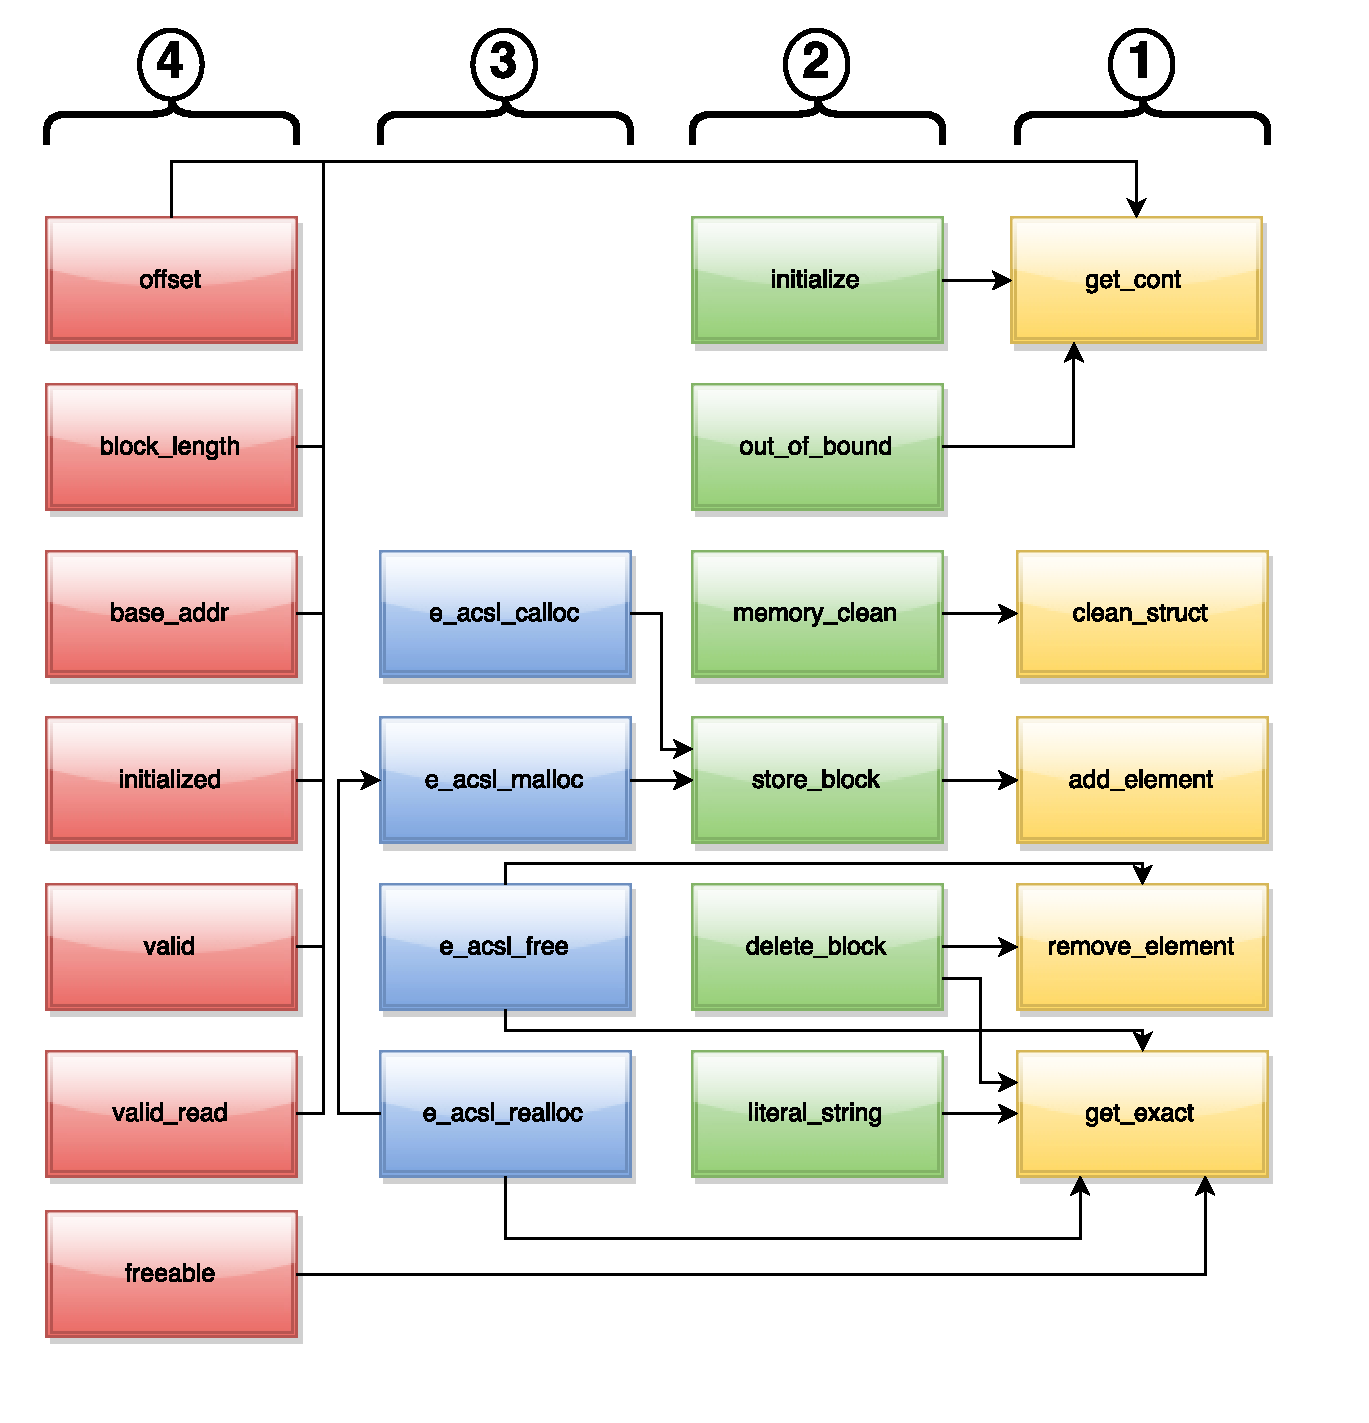
\includegraphics[scale=.55]{figures/mmodel_architecture.pdf}
  \vspace{-.8cm}
  \caption{Architecture de la bibliothèque de monitoring de la mémoire
    \label{fig:mmodel-architecture}}
\end{figure}

L'architecture comporte quatre niveaux, numérotés de \circled{1} à \circled{4}.
Les fonctions du niveau \circled{1} correspondent à l'implémentation de la
structure de données {\em store} (présentée au chapitre~\ref{sec:runtime})
gardant les informations à propos des blocs alloués.
Plusieurs implémentations sont fournies pour ces fonctions, correspondant à
différentes structures de données génériques : listes chaînées, arbres binaires
de recherche, Splay trees et Patricia tries.
Les fonctions du niveau \circled{2} servent à modifier le contenu du {\em store}
(ajout ou suppression d'élément, initialisation des éléments, etc.).
Les fonctions du niveau \circled{3} doivent être appelées en lieu et place des
fonctions de la bibliothèque standard associées (\lstinline'malloc', etc.).
Les fonctions du niveau \circled{4} permettent de calculer la valeur des
annotations \eacsl, elles retournent la valeur du terme ou du prédicat \eacsl
correspondant.
Ces fonctions ne modifient pas le contenu du {\em store}.

Les fonctions des niveaux \circled{2}, \circled{3} et \circled{4} sont
implémentées de manière indépendante à l'implémentation du {\em store} (niveau
\circled{1}).
Cette architecture facilite la conception des algorithmes, ainsi que la
comparaison d'efficacité des différentes implémentations du {\em store},
effectuée en partie~\ref{sec:eacsl-exp}.


\section{Expérimentations}
\label{sec:eacsl-exp}


Nous présentons maintenant le résultats de nos expérimentations visant à évaluer
la capacité de détection d'erreurs de la bibliothèque et la performance à
l'exécution des différents choix d'implémentation.


\subsection{Capacité de détection d'erreurs}


\begin{figure}
  \centering
  \begin{tabular}{c|c|c|c|c|c}
    & alarmes & mutants & équivalents & tués & \% erronés tués \\
    \hline
    fibonacci & 19  & 27 & 2 & 25 & 100\% \\
    \hline
    bubbleSort & 15  & 44 & 2 & 42 & 100\% \\
    \hline
    insertionSort & 10  & 39 & 3 & 36 & 100\% \\
    \hline
    binarySearch & 7 & 38 & 1 & 37 & 100\% \\
    \hline
    merge & 5 & 92 & 5 & 87 & 100\% \\
  \end{tabular}
  \caption{Capacité de détection d'erreurs
    \label{tab:mutation-exp}}
\end{figure}


Nous avons utilisé la technique de mutation pour évaluer la capacité de
détection d'erreurs en utilisant la vérification d'assertion à l'exécution avec
\framac.
Nous avons considéré 5 programmes écrits par nos soins.
Nous avons généré leurs {\em mutants} (en appliquant une {\em mutation} sur leur
code source) et leur avons appliqué la vérification à l'exécution.
Les mutations du programme incluent : modifications d'opérateur arithmétique
numérique, modifications d'opérateur arithmétique sur les pointeurs,
modifications d'opérateur de comparaison et modifications d'opérateur logique
($et$ et $ou$).
L'outil de génération de test \pathcrawler \cite{\citepathcrawler} a été
utilisé pour produire les cas de test.
Chaque mutant a été instrumenté par \eacsltoc et exécuté sur chaque cas de test
pour vérifier que la spécification était satisfaite à l'exécution.
Les programmes d'origine passent toutes les vérifications à l'exécution.
Lorsqu'une violation d'une annotation a été reportée pour au moins un cas de
test, le mutant est considéré comme étant {\em tué}.
La figure~\ref{tab:mutation-exp} présente les résultats.
La première colonne contient les exemples étudiés.
La deuxième colonne contient le nombre d'annotations dans chaque programme,
générées par interprétation abstraite (le greffon \Value a été utilisé).
Les colonnes suivantes contiennent le nombre de mutants générés, le nombre de
mutants équivalents, le nombre de mutants non-équivalents tués, et le
pourcentage des mutants non-équivalents tués lors de l'exécution.
Lors de ces expérimentations, tous les mutants non-équivalents erronés ont été
tués, ce qui témoigne de la précision et de la complétude de notre méthode.


\subsection{Performance des choix d'implémentation}


Pour évaluer la performance à l'exécution de notre implémentation de la
bibliothèque, nous avons effectué plus de 300 exécutions sur plus de 30
programmes, obtenus à partir d'une dizaine de programmes écrits et annotés par
nos soins.
Nous avons volontairement gardé des exemples plutôt courts (moins de 200 lignes
de code) car ils ont dû être annotés en \eacsl manuellement.

Nous avons mesuré le temps d'exécution du programme d'origine et du code
instrumenté par \eacsltoc avec différentes options, afin d'évaluer les
performances des différentes implémentations du {\em store} et des différentes
optimisations.
Des indicateurs comme le nombre de variables, d'allocations mémoires,
d'enregistrements et de requêtes ont également été enregistrés.


\textbf{Calcul du plus grand préfixe commun :} \\
Nous avons comparé deux implémentations de ce calcul, qui est utilisé par
l'implémentation du {\em store} utilisant des Patricia tries.
La première implémentation utilise un parcours linéaire de l'adresse (bit-à-bit,
de gauche à droite).
La seconde implémentation est une recherche dichotomique du meilleur préfixe
dans un tableau dont le contenu et les indices sont pré-calculés.
Elle implémente l'algorithme~\ref{algo:prefix} présenté en
partie~\ref{sec:mpgpc}.
Cette seconde implémentation s'est révélée en moyenne 2.7 fois plus rapide que
la première sur nos exemples.


\begin{figure}[h!]
  \begin{tikzpicture}
    \begin{axis}[axis y line=left,width=\textwidth,height=\textwidth,ymode=log,
        legend columns=2,xlabel={$N$},ylabel={temps (s.)}]
      \pgfplotstableread{data/table_eacsl_experiments_merge_sort.dat}
      \loadedtable;
      \addplot [color=red,ultra thick] table[x=N,y=list] {\loadedtable}
      node[above,pos=1] {list};

      \addplot [color=red,dashed,ultra thick]
      table[x=N,y=list-DFA] {\loadedtable}
      node[below,left,pos=1,yshift=-.5cm] {list-AS};

      \addplot [color=blue,ultra thick] table[x=N,y=bst] {\loadedtable}
      node[above,right,pos=1] {bst};

      \addplot [color=blue,dashed,ultra thick]
      table[x=N,y=bst-DFA] {\loadedtable}
      node[above,right,pos=1] {bst-AS};

      \addplot [color=greenv,ultra thick] table[x=N,y=Pt] {\loadedtable}
      node[above,left,pos=1,xshift=-1.4cm] {Pt};

      \addplot [color=greenv,dashed,ultra thick]
      table[x=N,y=Pt-DFA] {\loadedtable}
      node[above,left,pos=1] {Pt-dicho};

      \addplot [color=orange,ultra thick] table[x=N,y=Pt-opti] {\loadedtable}
      node[below,right,pos=1,yshift=-.5cm,xshift=-1.2cm] {Pt-AS};

      \addplot [color=orange,dashed,ultra thick]
      table[x=N,y=Pt-opti-DFA] {\loadedtable}
      node[above,left,pos=1] {Pt-dicho-AS};

      \addplot [color=violet,ultra thick] table[x=N,y=St] {\loadedtable}
      node[below,right,pos=1] {St};

      \addplot [color=violet,dashed,ultra thick]
      table[x=N,y=St-DFA] {\loadedtable}
      node[below,right,pos=1,yshift=-.7cm] {St-AS};

      %% \foreach \i in {
      %%   list,list-DFA,bst,bst-DFA,Pt,Pt-opti,Pt-DFA,Pt-opti-DFA,St,St-DFA} {
      %%   \addplot table [x=N, y=\i] {\loadedtable};
      %% }

      \legend{list,list-AS,bst,bst-AS,Pt,Pt-dicho,Pt-AS,Pt-dicho-AS,St,St-AS}
    \end{axis}
  \end{tikzpicture}
  \vspace{-.8cm}
  \caption{Comparaison du temps d'exécution des différentes implémentations du
    {\em store} sur un tri fusion
    \label{fig:mmodel-exp}}
\end{figure}


%% \begin{figure}[bt]
%%   \begin{tikzpicture}
%%     \begin{axis}[axis y line=left,width=\textwidth,height=\textwidth,ymode=log]
%%       \pgfplotstableread{data/table_eacsl_experiments_merge_sort.dat}
%%       \loadedtable;
%%       \foreach \i in {
%%         list,bst,Pt,Pt-opti,St} {
%%         \addplot table [x=N, y=\i] {\loadedtable};
%%       }
%%       \legend{list,bst,Pt$_1$,Pt$_2$,St}
%%     \end{axis}
%%   \end{tikzpicture}
%%   \caption{Comparaison des différentes implémentations du {\em store}
%%     \label{fig:mmodel-exp-2}}
%% \end{figure}


\textbf{Implémentation du {\em store} :}\\
Pour déterminer quelle implémentation du {\em store} est la plus appropriée,
nous avons comparé quatre implémentations utilisant : des Patricia tries, des
listes chaînées, des arbres binaires de recherche non équilibrés et des arbres
binaires de recherche équilibrés (Splay trees~\cite{Sleator/85}).

La figure~\ref{tab:mmodel-exp} présente les résultats des expérimentations
comparant les différentes implémentations du {\em store} et du calcul du plus
grand préfixe commun.
La première colonne du tableau contient les exemples étudiés.
$bS_{10000}$ est une recherche binaire dans un tableau de 10000 éléments.
$iS_{10000}$ est un tri par insertion d'un tableau de 10000 éléments.
$mM_{n^2}$ est une multiplication de matrices $n \times n$. mI$_{n^2}$ contient
des calculs matriciels (dont inversion et multiplication) sur des  matrices
$n \times n$.
$qS_n$ est un tri rapide sur un tableau de $n$ éléments.
$bbS_{10000}$ est un tri à bulle sur un tableau à 10000 éléments.
$m_{30000}$ est une fusion de deux listes chaînées de 10000 et 20000 éléments.
$Rbt_{10000}$ est une insertion/suppression de 10000 éléments dans un arbre rouge
et noir.
$mS_n$ est un tri fusion d'une liste chaînée de $n$ éléments.
La ligne supplémentaire ``+ RTE'' de chaque exemple correspond à une application
préalable du greffon \rte qui génère des assertions qui sont vraies si le
programme ne contient pas d'erreur à l'exécution.
Nous appelons ces assertions à vérifier des ``alarmes''.

La colonne $\danger$ contient le nombre d'alarmes du programme (générées par les
greffons \rte et \Value).
La colonne $\emptyset$ contient le temps d'exécution du programme original.
Tous les temps d'exécution sont mesurés en secondes.
Un temps d'exécution est noté $\infty$ quand il dépasse 24 heures.
Dans les colonnes suivantes, le suffixe ``-AS'' correspond aux expérimentations
avec application d'une analyse statique permettant de n'instrumenter que ce qui
est nécessaire (section 6 de \cite{\citeeacsltoc}).
Cette analyse n'étant pas le fruit de nos travaux, nous ne la présentons pas
ici.
La colonne $list$ contient le temps d'exécution du programme lorsque le
{\em store} est implémenté par une liste chaînée.
La colonne $bst$ contient le temps d'exécution du programme lorsque le
{\em store} est implémenté par un arbre binaire de recherche non équilibré.
La colonne $Pt$ contient le temps d'exécution du programme lorsque le
{\em store} est implémenté par un Patricia trie et lorsque la recherche du
masque du plus grand préfixe commun de deux adresses est implémentée de manière
linéaire.
La colonne $Pt-dicho$ contient le temps d'exécution du programme lorsque le
{\em store} est implémenté par un Patricia trie et lorsque la recherche du
masque du plus grand préfixe commun de deux adresses est implémentée en
utilisant l'algorithme~\ref{algo:prefix} présenté en partie~\ref{sec:mpgpc}.
La colonne $St$ contient le temps d'exécution du programme lorsque le
{\em store} est implémenté par un Splay tree.
Le temps d'analyse du programme sans instrumentation avec le débogueur
\valgrind~\cite{\citevalgrind} est indiqué dans la dernière colonne.

Nous remarquons que le temps d'exécution de \valgrind n'est pas comparable avec
celui de notre bibliothèque, cela s'explique simplement par le fait que celui-ci
ne prend pas en compte la spécification \eacsl, et se contente de vérifier des
propriétés comme l'absence d'erreur de segmentation ou l'absence de fuite de
mémoire.
En effet, notre démarche vise à supporter au maximum les annotations \eacsl,
ce qui nécessite un monitoring plus lourd.

La figure~\ref{fig:mmodel-exp} représente graphiquement le temps (en secondes)
passé par chaque implémentation du {\em store} sur un tri fusion de 1000, 5000,
10000, 50000 et 100000 éléments (les données chiffrées sont dans les cinq
dernières lignes de la figure~\ref{tab:mmodel-exp}).

Les résultats de nos expérimentations confirment nos hypothèses, à savoir :

\begin{itemize}
\item[\textbf{H1}]
  le Patricia trie est la structure de données la plus appropriée pour
  l'implémentation du {\em store};

\item[\textbf{H2}]
  notre optimisation de la recherche du masque du plus grand préfixe commun par
  recherche dichotomique et l'utilisation d'indices pré-calculés entraîne un
  vrai gain de performance;

\item[\textbf{H3}]
  l'utilisation d'une analyse statique visant à réduire l'instrumentation
  du programme permet de réduire le temps d'exécution de manière efficace.
\end{itemize}


Concernant \textbf{H1}, la figure~\ref{tab:mmodel-exp} montre que
l'implémentation du {\em store} par un Patricia trie est la plus efficace.
Elle est en moyenne 2500 fois plus rapide que l'implémentation à base de listes
chaînées, 200 fois plus rapide que celle utilisant les arbres binaires de
recherche, et 27 fois plus rapide que celle se basant sur les Splay trees.

La version utilisant les Splay trees offre des performances comparables (ou
légèrement meilleures, jusqu'à 3 fois) sur les exemples contenant de fréquents
accès mémoire consécutifs au même bloc dans le {\em store}, comme c'est le cas
du tri fusion (voir la figure~\ref{fig:mmodel-exp}).
En revanche, sur des exemples où les accès mémoire consécutifs ne se font pas
sur le même bloc (une multiplication de matrices dans notre exemple), les
performances sont beaucoup moins bonnes (jusqu'à 500 fois).
Ceci est dû à la nature des Splay trees : le dernier élément accédé est remonté
à la racine de l'arbre.

Concernant \textbf{H2}, la figure~\ref{tab:mmodel-exp} montre que la version
dichotomique de la recherche du masque du plus grand préfixe commun est toujours
plus efficace qu'une recherche linéaire.
Elle est en moyenne 3 fois plus rapide que cette dernière.

Concernant \textbf{H3}, nos résultats montrent que l'utilisation d'une analyse
statique visant à réduire l'instrumentation du programme entraîne un gain de
performance.
En effet, pour chacune des implémentations du {\em store}, l'analyse statique
permet de réduire le temps d'exécution.
L'exécution après analyse statique peut être jusqu'à 200 fois plus rapide sur
certains exemples.
Elle permet notamment de ne pas observer de {\em timeout} pour les listes
chaînées et les arbres binaires de recherche sur l'exemple du tri fusion de
50000 éléments.


\section*{Conclusion du chapitre}


Dans ce chapitre nous avons présenté l'architecture de l'implémentation de la
bibliothèque de monitoring de la mémoire, dont les algorithmes et les principes
théoriques ont été traités dans le chapitre~\ref{sec:runtime}.

Nous avons présenté les résultats de nos expérimentations visant à
mesurer la capacité de détection d'erreurs et les performances à l'exécution de
notre implémentation.
Nous avons notamment comparé les performances de quatre implémentations du
{\em store}.
Nous avons également comparé deux implémentations de la recherche du masque du
plus grand préfixe commun, dans le cas où le {\em store} est implémenté en
utilisant un Patricia trie.
Enfin, nous avons mesuré l'impact de l'utilisation d'une analyse statique visant
à réduire l'instrumentation du programme (section 6 de \cite{\citeeacsltoc}),
pour chacune des implémentations du {\em store}.
Nos expérimentations ont mis en avant l'efficacité d'une implémentation du
{\em store} à base de Patricia trie.
Elles ont également montré qu'une recherche du masque du plus grand préfixe
commun par dichotomie (l'algorithme est présenté en partie~\ref{sec:mpgpc}) est
plus efficace qu'une recherche linéaire et que l'analyse statique permet
effectivement de réduire le temps de la vérification à l'exécution.

Le travail réalisé a permis de concevoir une méthode et un outil de vérification
à l'exécution des annotations \eacsl portant sur le modèle mémoire.
Nos travaux ont permis de déterminer expérimentalement quelles implémentations
du {\em store} et des différents algorithmes sont les plus efficaces pour notre
outil de vérification.
L'implémentation du {\em store} à base de Patricia trie et les différents
algorithmes présentés dans ce chapitre et dans le chapitre~\ref{sec:runtime}
sont intégrés à l'outil \eacsltoc~\cite{\citeeacsltoc}.


\begin{landscape}
  \begin{figure}[h]
    \centering
    \begin{footnotesize}
      \begin{tabular}{l|c|c|c|c|c|c|c|HHc|c|HHc|c|c|c}
  & $\danger$ & $\emptyset$ & list & list-AS & bst & bst-AS & Pt & mask$^1$ & sb$^1$ & Pt-dicho & Pt-AS & mask$^2$ & sb$^2$ & Pt-dicho-AS & St & St-AS & valgrind \\
  \hline
  bS$_{10000}$ &22 &\multirow{2}{*}{.01} &1.10 &0.50 &1.14 &0.64 &1.55 &99 &16 &1.55 &0.57 &0 &1 &0.55 &1.39 &0.61 &\multirow{2}{*}{0.27}\\
  + RTE &41 &&1.10 &0.51 &1.14 &0.62 &1.59 &109 &16 &1.59 &0.53 &0 &1 &0.53 &1.39 &0.64 &\\
  \hline
  iS$_{10000}$ &5 &\multirow{2}{*}{.12} &2.29 &0.12 &1.83 &0.12 &2.89 &170k &20k &2.91 &0.12 &0 &0 &0.12 &2.46 &0.12 &\multirow{2}{*}{2.81}\\
  + RTE &24 &&3.52 &1.27 &2.89 &1.26 &3.99 &170k &20k &3.86 &1.25 &0 &0 &1.25 &3.46 &1.30 &\\
  \hline
  mM$_{100^2}$ &0 &\multirow{2}{*}{.01} &2.29 &0.73 &2.94 &1.15 &0.14 &17k &1k &0.14 &0.10 &5k &612 &0.09 &1.07 &0.98 &\multirow{2}{*}{0.34}\\
  + RTE &82 &&13.17 &10.66 &21.92 &17.39 &2.78 &18k &1k &3.00 &2.64 &5k &612 &2.82 &75.97 &73.62 &\\
  \hline
  mM$_{150^2}$ &0 &\multirow{2}{*}{.01} &13.23 &3.96 &15.65 &6.20 &0.54 &21k &2k &0.51 &0.36 &9k &912 &0.35 &5.86 &5.64 &\multirow{2}{*}{0.48}\\
  + RTE &82 &&72.36 &58.48 &110.70 &90.43 &10.77 &24k &2k &9.01 &8.57 &9k &912 &8.75 &403.50 &398.60 &\\
  \hline
  mI$_{100^2}$ &2 &\multirow{2}{*}{.01} &22.51 &0.10 &7.74 &0.13 &0.09 &68k &5k &0.08 &0.01 &7k &609 &0.01 &0.19 &0.10 &\multirow{2}{*}{0.35}\\
  + RTE &155 &&28.96 &4.22 &13.67 &5.48 &0.54 &73k &5k &0.55 &0.53 &7k &611 &0.47 &26.37 &26.16 &\\
  \hline
  mI$_{150^2}$ &2 &\multirow{2}{*}{.02} &130.04 &0.34 &40.35 &0.45 &0.28 &99k &8k &0.27 &0.02 &12k &909 &0.02 &0.68 &0.34 &\multirow{2}{*}{0.47}\\
  + RTE &155 &&153.30 &21.54 &73.55 &29.94 &2.00 &105k &8k &1.90 &1.42 &12k &911 &1.53 &146.15 &145.80 &\\
  \hline
  qS$_{1000}$ &15 &\multirow{2}{*}{.01} &12.70 &2.08 &1.76 &0.59 &0.33 &1M &92k &0.06 &0.13 &683k &39k &0.02 &0.02 &0.01 &\multirow{2}{*}{0.27}\\
  + RTE &32 &&12.38 &2.13 &1.64 &0.56 &0.38 &1M &92k &0.12 &0.14 &727k &39k &0.04 &0.03 &0.02 &\\
  \hline
  qS$_{2000}$ &15 &\multirow{2}{*}{.01} &85.99 &11.31 &8.39 &2.78 &0.71 &3M &198k &0.14 &0.28 &1M &84k &0.05 &0.03 &0.02 &\multirow{2}{*}{0.27}\\
  + RTE &32 &&81.65 &11.15 &7.72 &2.67 &1.13 &4M &198k &0.48 &0.36 &1M &84k &0.13 &0.05 &0.02 &\\
  \hline
  bbS$_{10000}$ &4 &\multirow{2}{*}{.22} &13.78 &1.02 &16.84 &1.67 &117.47 &499M &49M &22.36 &1.57 &30 &7 &1.54 &8.80 &1.67 &\multirow{2}{*}{3.36}\\
  + RTE &16 &&23.08 &4.64 &30.69 &7.16 &107.05 &599M &49M &32.58 &7.26 &29 &7 &6.90 &17.29 &7.21 &\\
  \hline
  m$_{30000}$ &2 &\multirow{2}{*}{.01} &412.10 &11.38 &176.35 &11.01 &1.11 &5M &420k &0.26 &0.30 &1M &60k &0.06 &0.08 &0.01 &\multirow{2}{*}{0.45}\\
  + RTE &49 &&451.58 &101.33 &219.12 &94.80 &1.15 &5M &420k &0.29 &0.47 &2M &130k &0.14 &0.10 &0.05 &\\
  \hline
  Rbt$_{10000}$ &0 &\multirow{2}{*}{.01} &47.39 &0.28 &48.44 &0.27 &0.32 &1M &159k &0.09 &0.03 &151k &10k &0.01 &0.59 &0.01 &\multirow{2}{*}{0.51}\\
  + RTE &270 &&120.02 &101.69 &165.77 &145.20 &0.47 &1M &159k &0.30 &0.39 &979k &119k &0.27 &18.82 &19.59 &\\
  \hline
  mS$_{1000}$ &7 &\multirow{2}{*}{.01} &6.45 &0.34 &6.32 &0.11 &0.32 &1M &95k &0.07 &0.06 &331k &18k &0.01 &0.02 &0.01 &\multirow{2}{*}{0.27}\\
  + RTE &45 &&6.82 &1.35 &7.98 &0.38 &0.34 &1M &95k &0.10 &0.13 &701k &38k &0.04 &0.02 &0.01 &\\
  \hline
  mS$_{5000}$ &7 &\multirow{2}{*}{.01} &362.87 &11.00 &218.01 &3.43 &2.28 &11M &562k &0.76 &0.43 &2M &106k &0.09 &0.14 &0.03 &\multirow{2}{*}{0.27}\\
  + RTE &45 &&371.40 &50.94 &290.88 &10.34 &2.46 &11M &562k &0.80 &0.83 &4M &218k &0.22 &0.16 &0.08 &\\
  \hline
  mS$_{10000}$ &7 &\multirow{2}{*}{.01} &3624.01 &47.94 &1673.00 &16.10 &6.46 &23M &1M &2.75 &1.00 &5M &223k &0.21 &0.31 &0.08 &\multirow{2}{*}{0.27}\\
  + RTE &45 &&3406.43 &257.18 &2086.32 &46.22 &6.30 &23M &1M &2.66 &1.83 &9M &457k &0.51 &0.35 &0.18 &\\
  \hline
  mS$_{50000}$ &7 &\multirow{2}{*}{.01} &$\infty$ &3847.72 &$\infty$ &1100.93 &135.54 &146M &6M &111.22 &6.90 &33M &1M &1.65 &2.08 &0.58 &\multirow{2}{*}{0.63}\\
  + RTE &45 &&$\infty$ &25554.08 &$\infty$ &2781.90 &118.86 &145M &6M &95.74 &11.64 &54M &2M &3.37 &2.18 &1.15 &\\
  \hline
  mS$_{100000}$ &7 &\multirow{2}{*}{.01} &$\infty$ &$\infty$ &$\infty$ &$\infty$ &631.41 &296M &14M &559.93 &13.55 &70M &2M &3.35 &4.03 &1.15 &\multirow{2}{*}{0.27}\\
  + RTE &45 &&$\infty$ &$\infty$ &$\infty$ &$\infty$ &573.47 &308M &14M &513.85 &25.02 &116M &5M &7.63 &4.68 &2.50 &\\
\end{tabular}

    \end{footnotesize}
    \caption{Comparaison des différentes implémentations du {\em store}
      \label{tab:mmodel-exp}}
  \end{figure}
\end{landscape}


\chapter{Greffon Statique-Dynamique (StaDy)}
\label{sec:stady}

\chapterintro

TODO


\section{Implémentation}


%\begin{landscape}
\begin{center}
  \begin{figure}
    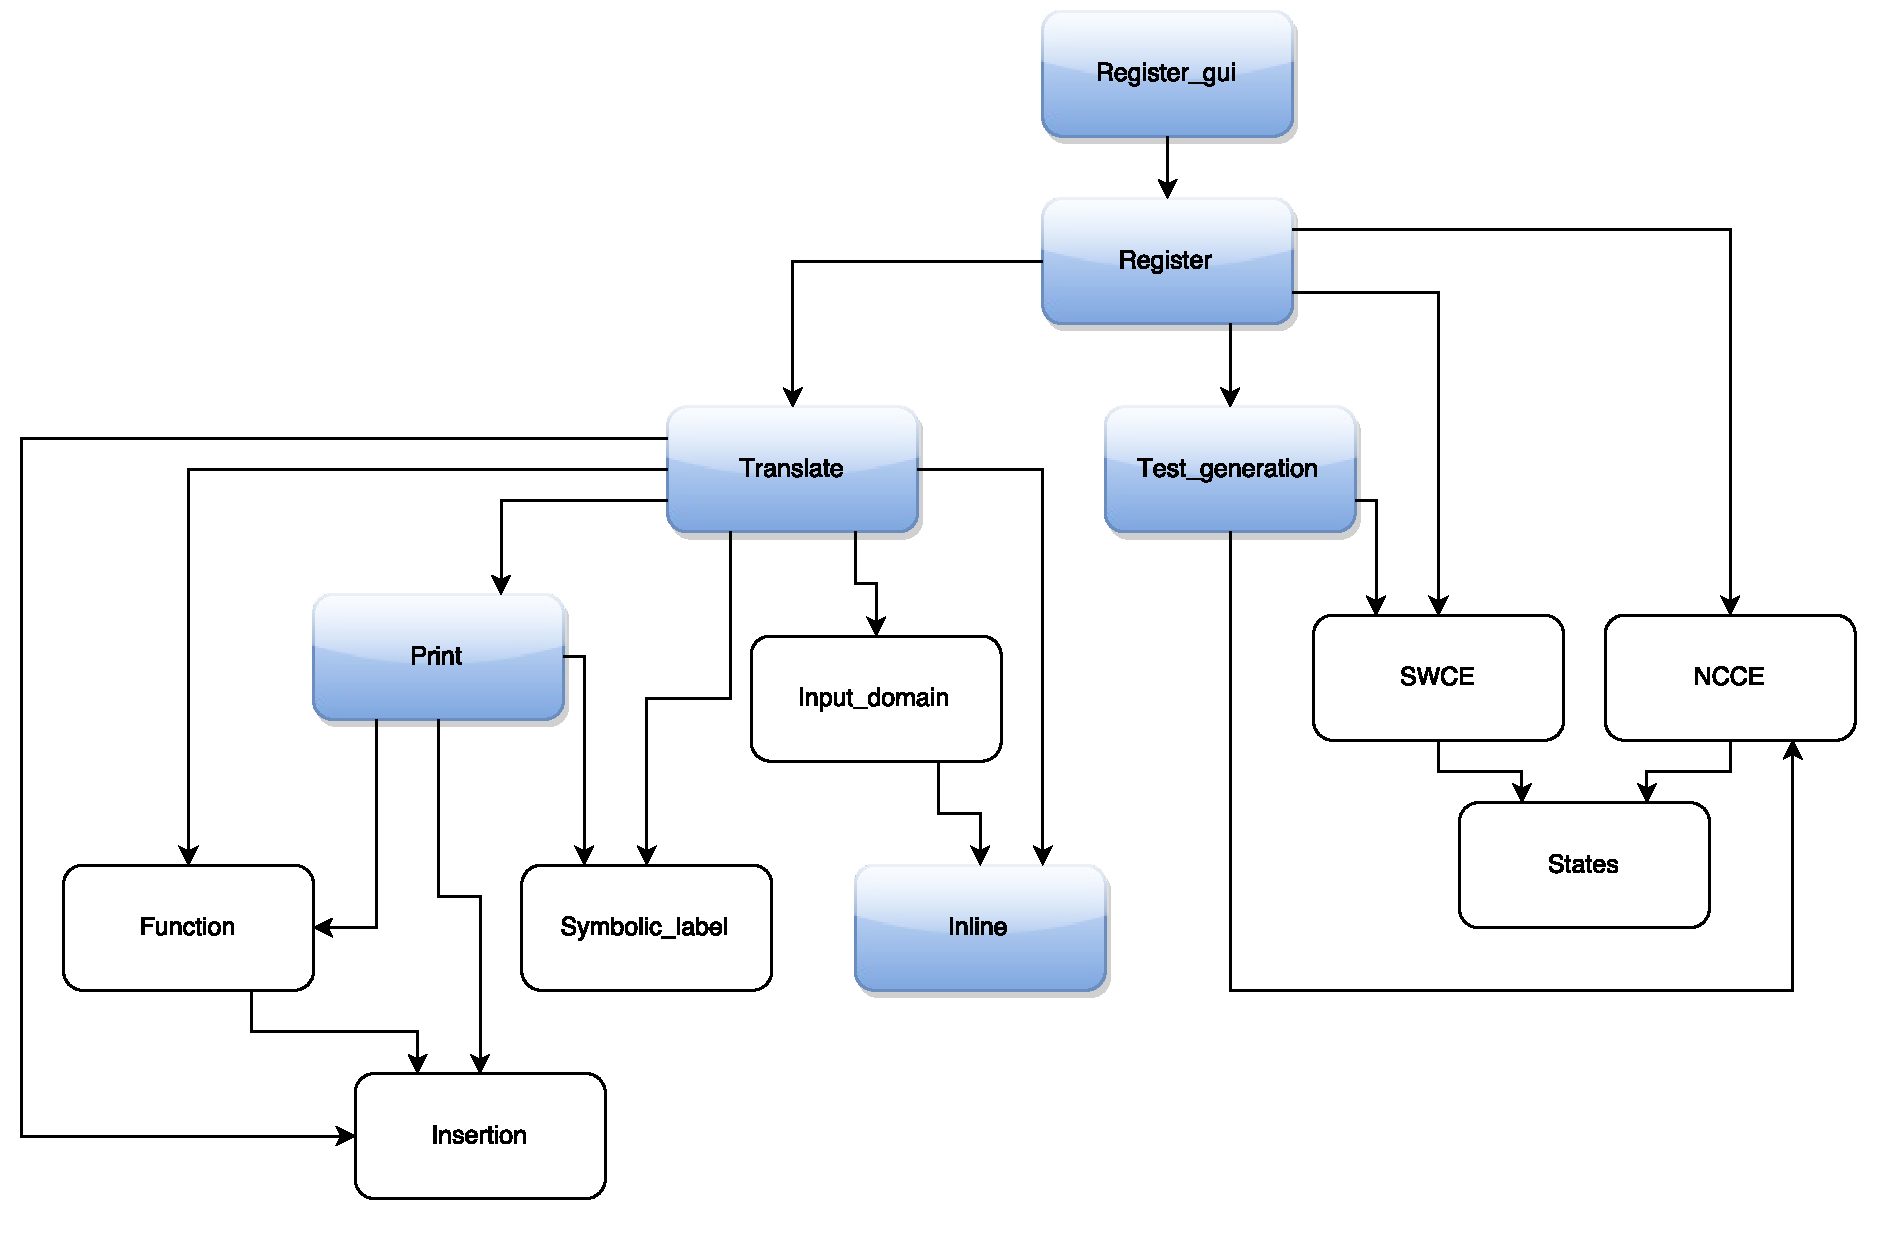
\includegraphics[scale=.5]{figures/stady_architecture.pdf}
    \vspace{-11cm}
    \caption{Architecture de \textsc{StaDy}
      \label{fig:stady-architecture}}
  \end{figure}
\end{center}
%\end{landscape}


\section{Expérimentations}


\begin{figure}[tb]\scriptsize
  %\vspace{-2mm}
  \begin{center}
    \begin{tabular}{lrr}
      \hline
      example & time (s.) & \# paths \\ \hline
      array-unsafe & 1.299 & 9 \\ \hline
      count-up-down-unsafe & 1.285 & 3 \\ \hline
      eureka-01-unsafe & 1.355 & 48 \\ \hline
      for-bounded-loop1-unsafe & 1.320 & 11 \\ \hline
      insertion-sort-unsafe & 16.530 & 730 \\ \hline
      invert-string-unsafe & 1.359 & 48 \\ \hline
      linear-search-unsafe & 3.624 & 2766 \\ \hline
      matrix-unsafe & 1.367 & 22 \\ \hline
      nec20-unsafe & 1.463 & 1035 \\ \hline
      string-unsafe & 1.362 & 48 \\ \hline
      sum01-bug02-base-unsafe & 1.335 & 26 \\ \hline
      sum01-bug02-unsafe & 1.327 & 36 \\ \hline
      sum01-unsafe & 1.312 & 56 \\ \hline
      sum03-unsafe & 1.291 & 46 \\ \hline
      sum04-unsafe & 1.310 & 22 \\ \hline
      sum-array-unsafe & 1.358 & 14 \\ \hline
      %% trex01-unsafe & 1.561 \\ \hline
      trex03-unsafe & 1.358 & 21 \\ \hline
      sendmail-unsafe & 1.396 & 77 \\ \hline
      vogal-unsafe & 1.349 & 341 \\ \hline
    \end{tabular}
  \end{center}
  \vspace{-3mm}
  \caption{Experiments with \textsc{StaDy}: Bug detection}    
  \label{fig:scam-experiments1}
  \vspace{-3mm}
\end{figure}

\begin{figure}[tb]\scriptsize
  %\vspace{-2mm}
  \begin{center}
    \begin{tabular}{lrrrr}
      \hline
      example & mutants & $\lnot$ equiv. & killed & success rate \\ \hline
      merge-sort & 96  & 92 & 88 & 95.65\% \\ \hline
      merge-arrays & 68 & 63 & 59 & 93.65\% \\ \hline
      quick-sort & 130 & 130 & 130 & 100\% \\ \hline
      binary-search & 40 & 40 & 39 & 97.5\% \\ \hline
      bubble-sort & 52 & 49 & 42 & 85.71\% \\ \hline
      insertion-sort & 39 & 37 & 36 & 97.3\% \\ \hline
      array-safe & 18 & 16 & 15 & 93.75\% \\ \hline
      bubble-sort-safe & 64 & 58 & 55 & 94.83\% \\ \hline
      count-up-down-safe & 14 & 13 & 13 & 100\% \\ \hline
      eureka-01-safe & 60 & 60 & 60 & 100\% \\ \hline
      eureka-05-safe & 36 & 36 & 36 & 100\% \\ \hline
      insertion-sort-safe & 43 & 41 & 40 & 97.56\% \\ \hline
      invert-string-safe & 47 & 47 & 47 & 100\% \\ \hline
      linear-search-safe & 19 & 17 & 16 & 94.12\% \\ \hline
      matrix-safe & 30 & 27 & 25 & 92.59\% \\ \hline
      nc40-safe & 20 & 20 & 20 & 100\% \\ \hline
      nec40-safe & 20 & 20 & 20 & 100\% \\ \hline
      string-safe & 65 & 65 & 65 & 100\% \\ \hline
      sum01-safe & 14 & 14 & 13 & 92.86\% \\ \hline
      sum02-safe & 14 & 14 & 11 & 78.57\% \\ \hline
      sum03-safe & 10 & 10 & 10 & 100\% \\ \hline
      sum04-safe & 14 & 14 & 10 & 71.43\% \\ \hline
      sum-array-safe & 17 & 17 & 15 & 88.24\% \\ \hline
      trex03-safe & 56 & 56 & 56 & 100\% \\ \hline
      sendmail-safe & 31 & 31 & 31 & 100\% \\ \hline
      vogal-safe & 71 & 68 & 67 & 98.53\% \\ \hline
      \textbf{Total} & 1088 & 1054 & 1019 & \textbf{96.68\%} \\ \hline
    \end{tabular}
  \end{center}
  \vspace{-3mm}
  \caption{Experiments with \textsc{StaDy}: Mutation testing}
  \label{fig:scam-experiments2}
  \vspace{-3mm}
\end{figure}

The current implementation of  
\textsc{StaDy} supports a significant subset of \eacsl including
assertions, pre- and postconditions, loop invaliants and variants,
quantifications, logic functions, integral and pointer types, and
basic pointer operations. Pointer validity is currenty supported
only for input arrays and pointers.
\textsc{StaDy} currently  does not support 
\lstinline{assigns} clauses, \lstinline{\at} terms, 
real numbers, as well as advanced memory-related constructs
(e.g. \lstinline{\offset}), complex pointer
arithmetics such as \lstinline'p1-p2' or \lstinline'*(p-i)' and dynamic memory allocation  
due to the limitations of the underlying test generator. 
%Annotations involving reals
%($\mathbb{R}$) are not supported either.

To evaluate the efficiency of \textsc{StaDy} 
%to find counter-examples 
in a combined verification approach
(cf Sec. \ref{sec:motivations}),
we applied it on safe and unsafe programs from the TACAS 2014
Software Verification Competition%
\footnote{\url{https://svn.sosy-lab.org/software/sv-benchmarks/trunk/c/loops}}
%(selected from the subdirectory {\em loops})
%to evaluate its efficiency. 
First, we 
%tracked down bugs in faulty programs.
%We 
executed \textsc{StaDy} on 20 faulty programs that  handle arrays
with loops. The properties to invalidate originally 
expressed as C assertions, were manually rewritten in \textsc{E-ACSL}.
Adequate \textsc{E-ACSL} preconditions were also added. The programs
containing infinite loops and reachability properties to invalidate are not
handled by  \textsc{StaDy} due to the necessity to execute the program in
\textsc{Path\-Crawler}.
\textsc{Sta\-Dy}
 detected failures of all faulty properties in each considered program. 
Fig.~\ref{fig:scam-experiments1} illustrates the time taken to
invalidate the properties including all the steps of \textsc{Sta\-Dy}:
instrumentation from the \textsc{E-ACSL} specifications and test generation in
\textsc{PathCrawler}, and the number of explored paths.

Secondly, we used  mutation testing to evaluate the ability of \textsc{StaDy} to
find bugs in unsafe programs. % automatically generated from safe programs.
We selected 20 safe programs of the same benchmark, and 6
additional safe programs from our own benchmarks. All of them were annotated in
\textsc{E-ACSL}. They contain preconditions, postconditions, assertions,
memory-related properties, loop variants and invariants. We used mutation testing
on these safe programs to generate modified programs (\emph{mutants}) and see if
\textsc{StaDy} is able to \emph{kill} 
(i.e. to find errors in) these mutants. The
mutations performed on the source code mimic usual programming errors. They
include modifications of numerical and/or pointer arithmetic operators,
comparison operators, condition negation and logical operators ({\em and} and
{\em or}). Fig.~\ref{fig:scam-experiments2} gives the 
numbers of all and erroneous mutants, as well as 
the number and proportion of erroneous mutants killed by \textsc{StaDy}. 
\textsc{StaDy} showed 
an average success rate of 96.68\%, going up to 100\% on many examples.
The missing percents are mostly due to 
%the incompleteness of the specifications
%in some programs, explained by 
a currently incomplete support of \textsc{E-ACSL} features
by the underlying test generation tool.


%%%%%%%%%%%%%%%%%%%%%%%%%%%%%%%%%%%%%%%%%%%%%%%%%%%%%%%%%%%%

\begin{figure*}[bt]
  \scriptsize
\mbox{}\hspace{-20mm}
  \begin{center}
  \begin{tabular}{r|c|c|c|c|c|c|c|c|c|c|c|c|c|c|c}
    &&\multicolumn{3}{c|}{Proof}&\multicolumn{4}{c|}{\NCD}
    &\multicolumn{4}{c|}{\CWD}&\multicolumn{2}{c|}{$\NCD+\CWD$}&\\
    \hline
    \input{full_exp_latex_IEEE.csv}
  \end{tabular}
\end{center}
  \caption{Detailed experiments of proof failure diagnosis for mutants with \stady}
  \vspace{-.5cm}
  \label{tab:exp}
\end{figure*}


\textbf{Implementation.}
The proposed method for diagnosis of proof failures 
% detecting  non-compliances and contract weaknesses
%described in Sec.~\ref{sec:global-method} 
has been implemented as a \framac plugin, named \stady.
It relies on other plugins: \Wp~\citeframac for deductive
verification and \pathcrawler~\citepathcrawler for structural test generation.
\stady currently supports a significant subset of the \eacsl specification
language, including 
\lstinline'requires', \lstinline'ensures', 
\lstinline'behavior', \lstinline'assumes', 
\lstinline'loop invariant', \lstinline'loop variant' and
\lstinline'assert' clauses.
Quantified predicates
\lstinline[style=c]'\exists' and \lstinline[style=c]'\forall' and builtin terms
as \lstinline'\sum' or \lstinline'\numof' are translated as loops. 
Logic functions and named predicates are treated by inlining.
The \lstinline'\old' constructs are treated by saving the initial
values of formal parameters and global variables at the beginning of the
function. 
Validity checks of pointers are
partially supported due to the current limitation of the underlying test
generator: we can only check the validity of input pointers and global arrays.
The \lstinline'assigns' clauses are only taken into consideration during the
\CWD phase: we do not aim to find what is missing in the \lstinline'assigns'
clause (\NCD) because provers usually give sufficiently good feedback about it,
but we want to find what is unnecessary and could be removed from an
\lstinline'assigns' clause (\CWD).
Inductive predicates, recursive functions and floating-point numbers are
currently not supported and are part of our future work.

\textbf{The research questions} we address in our experiments are the following.

\vspace{-2mm}
\begin{itemize}
\item[\textbf{RQ1}]
Is \stady able to precisely diagnose most proof failures in C programs?
\item[\textbf{RQ2}]
What are the benefits of the \CWD extension (in particular, with respect to
\NCD)?
\item[\textbf{RQ3}]
Is \stady able to generate  \NCCE{}s or \CWCE{}s even with a partial testing coverage?
\item[\textbf{RQ4}]
Is \stady's execution time comparable to the time of an automatic proof?
\end{itemize}
\vspace{-2mm}



\textbf{Experimental protocol.} 
The evaluation used 20 annotated programs from \cite{ACSLbyExample},
whose size varies from 35 to 100 lines of annotated C code.
%binary\_search, binary\_search2, lower\_bound, upper\_bound, max\_element,
%max\_element2, max\_seq, min\_element, copy, fill, iota, replace\_copy,
%reverse\_copy, adjacent\_find, equal, equal2, equal3, find, find2 and mismatch.
These programs manipulate arrays, they are fully specified in \acsl and their
specification expresses non-trivial properties of C arrays. 
To evaluate the method
presented in Sec.~\ref{sec:global-method} and its implementation, we apply \stady on systematically
generated altered  versions (or \emph{mutants}) of correct C programs.
%We apply the method presented in Sec.~\ref{sec:method} and measure the
%efficiency of the classification performed by \stady.
%Each utants are generated for each considered program 
Each mutant program is obtained by performing a single modification (or \emph{mutation}) on the
initial program.
The mutations include: a binary operator modification in the code or in the
specification, a condition negation in the code, a relation modification in the
specification, a predicate negation in the specification, a partial loop invariant or
postcondition deletion in the specification.
In this study, we do not mutate the precondition of the function under verification, 
and restrict possible mutations on binary operators to avoid creating absurd
expressions, in particular for pointer arithmetics.


The first step tries to prove each mutant using \Wp. 
%(with a timeout high enough \commentNK{preciser}).
The proved mutants respect the specification and are classified as correct. 
% are equivalent to the original program. % NK: Not sure!
Second, we apply the \NCD method on the remaining mutants.
It classifies proof failures for some mutants as non-compliances, indicates the failing annotation and an \NCCE.
The third step applies the \CWD method on remaining mutants,
classifies some of them as subcontract weaknesses, indicates the weak subcontract and a \CWCE.
If no counter-example has been found by the \CWD, the mutant remains 
unclassified. % (the \textsf{?} column).
%\commentNK{preciser timeouts here}
The results are displayed in Fig.~\ref{tab:exp}.
The columns 
%of  Fig.~\ref{tab:exp}  
present the number of generated mutants, and the results of each of the three
steps: the number (\#) and ratio (\%) of classified mutants,
maximal and average execution time (put on two lines) of the step
over classified mutants ($t^\text{\ok}$ or $t^\text{\ko}$) and over non-classified
mutants ($t^\text{?}$) at this step.
The ratios are computed with respect to unclassified mutants after the previous step.
The $\NCD+\CWD$ columns sum up selected results after both $\NCD$ and $\CWD$ steps:
the average and maximal time ($t$) are shown globally over all mutants.
The time is computed until the proof is finished or until the first counter-example is generated.
The final number of remaining unclassified mutants (\#?) is given in the last column.


\textbf{Experimental results.}
%\textbf{RQ1.}
%Regarding RQ1,
For the 20 considered programs, 928 mutants have been generated. 80 of them 
%are equivalent and 
have been proved by \Wp.
Among the 848 unproven mutants, \NCD has detected a non-compliance
induced by the mutation in 776 mutants (91.5\%),
leaving 72 unclassified.
Among them, \CWD has been able to exhibit a counter-example (either a \NCCE or a
\CWCE)
%, the confirmation step is not automatized yet) %NK: to be done for the final version
%for the contract impacted by
%the mutation in
for 48 of them (66.7\%), finally leaving 24 programs unclassified.
They can be either equivalent mutants that were not proved
by \Wp due to a prover incapacity, or mutants coming from a mutation 
in an unsupported annotation being undetectable by the
current version, or incorrect mutants for which testing was incomplete due to a timeout.
Regarding \textbf{RQ1}, \stady has found a precise reason
of the proof failures  and produced a counter-example 
in 824 of the 848 unproven mutants, 
i.e. classifying 97.2\%.
Exploring the benefits of detecting a prover incapacity may often require to manually reduce
the input domain, to try additional lemmas or interactive proof, so it   
was not sufficiently investigated in this study 
(and would probably require another, non mutational approach).

%\textbf{RQ2.}
Regarding \textbf{RQ2}, 
\NCD alone diagnosed 776 of 848 unproven mutants (91.5\%).
\CWD diagnosed 48 of the 72 remaining  mutants (66.7\%)
bringing a significant complementary contribution 
to a better understanding of reasons of many proof failures.
%The combined efforts of \NCD and \CWD classified 824 of 848 non-equivalent mutants
%(97.2\%), so \CWD permitted to add roughly 6\% to the fault detection efficiency
%of \NCD.

%\textbf{RQ3.}
In our experiments,
each prover can try to prove each verification condition 
%proof obligation 
during at most 40 seconds.
We also set a timeout for any test generation session
to 5 seconds, i.e. one session for the \NCD step, and 
several sessions for \CWD steps.
We also limit the depth of explored program paths with the 
{\em k-path} criterion (cf. Sec. \ref{sec:framac})
%With this option, the test generator only considers paths with at most
%$k$ consecutive iterations of each loop. 
setting $k = 4$.
Both the session timeout and the {\em k-path} heavily limit the testing coverage
but \stady still detects 97.2\% of faults in the generated programs.
That addresses \textbf{RQ3} and demonstrates that the proposed method can efficiently 
classify proof failures and generate counter-examples
even with a partial testing coverage and can therefore 
be used for programs where the 
total number of paths cannot be limited
(e.g. by the \lstinline{typically} clause).

%\textbf{Time of analysis.}
Concerning \textbf{RQ4},
on the considered programs \Wp needs on average 2.6 sec. per mutant (at most 4.4 sec.) to
prove a program, and spends 13.0 sec. on average (at most 61.3 sec.) when the
proof fails.
The total execution time of \stady is comparable: it needs on average 2.7 sec.  per unproven mutant 
(at most 19.9 sec.).
%More precisely, the \NCD step needed 2.4 sec. on average (at most 9.4 sec.) to
%detect a non-compliance, and on average 2.5 sec. (at most 8.3 sec.) when it is
%non conclusive.
%The \CWD step needed 2.4 sec. on average (at most 6.4 sec.) to
%detect a contract weakness, and on average 6.3 sec. (at most 11.6 sec.) when it
%is non conclusive.

\textbf{Summary.}
The experiments show that the proposed method can automatically classify a significant number
of proof failures within an analysis time comparable to the time of an automatic proof
and for programs for which only a partial testing coverage is possible.
The \CWD technique offers an efficient complement to \NCD for a more 
complete and more precise diagnosis of proof failures.

\textbf{Threats to validity.}
As it is often the case in software verification studies, one major threat is
related to the 
representativeness of results, i.e. their \textit{external validity}.
In our case, due to the nature of the problem,
we are restricted to realistic annotated programs
that cannot be generated automatically 
or extracted from existing databases of unspecified code.
Therefore, to reduce this threat, we used programs from an \textit{independent}
benchmark \cite{ACSLbyExample} created in order to illustrate
on different examples the usage of the \acsl specification 
language for deductive verification with \framac.


%Though, the primary contribution of this article is to propose 
%a novel classification of proof failures and techniques
%for their classification.

\textit{Scalability} of the results is another threat
since we do not demonstrate their validity for functions of larger programs. 
%While this is an important issue we plan to address in the near future, 
%However,  
Because of the modular reasoning of deductive verification,
it can be argued that the proposed technique should only be applied on a unit level,
separately for each function, since the verification engineer proves a program  in this way.
Indeed, in the current practice of deductive verification, it does not make sense to analyze
proof failures for the whole module or application at the same time.

The main scalability concern is thus related to the usage of structural test generation 
that can often time out without achieving a full coverage.
To address this issue, we have specifically investigated the impact of a partial test coverage
on the effectiveness of the method (cf. \textbf{RQ3} above) and proposed
a convenient way to reduce the input domain (using \lstinline{typically} clause, 
an extension of \acsl).

Other threats can be due to the used measurements, i.e. \textit{construct validity}.
To reduce this threat, we used a careful measurement of 
results (including analysis time for each step and 
each mutant, their mean and maximal values, 
separately computed for classified and unclassified proof failures).
One concern is producing realistic situations in which 
the verification engineer can need help in the analysis of proof failures.
While the first users of \stady have appreciated its feedback, % \cite{ggp15},
we have not yet had the opportunity to organize a fair evaluation with a 
representative group of users. 
Thus we have performed an extended set of experiments using simulation of 
errors by mutations as an alternative in the meanwhile. 
We have chosen a large subset of mutation operators (mutation in the code,
mutation in an annotation, deletion of an annotation) that model 
frequent problematic situations 
(incorrect code or annotations, incomplete specification)
leading to proof failures.
This approach looks suitable for non-compliance and subcontract weaknesses, and
certainly less suitable for the more subtle prover incapacity cases.
The results should be later confirmed by a representative user study.


\section*{Conclusion du chapitre}


TODO



\part{Conclusion}
\chapter{Bilan}
TODO
\chapter{Perspectives}
TODO


\backmatter

\bibliographystyle{phdthesisapa}
\bibliography{biblio}

\listoffigures
\listoftables
\listofdefinitions
\listofmypropertys

\appendix
\part{Annexes}

\chapter{Premier chapitre des annexes}
\chapter{Second chapitre des annexes}

\end{document}

